\documentclass[twoside]{book}

% Packages required by doxygen
\usepackage{calc}
\usepackage{doxygen}
\usepackage{graphicx}
\usepackage[utf8]{inputenc}
\usepackage{makeidx}
\usepackage{multicol}
\usepackage{multirow}
\usepackage{textcomp}
\usepackage[table]{xcolor}

% Font selection
\usepackage[T1]{fontenc}
\usepackage{mathptmx}
\usepackage[scaled=.90]{helvet}
\usepackage{courier}
\usepackage{amssymb}
\usepackage{sectsty}
\renewcommand{\familydefault}{\sfdefault}
\allsectionsfont{%
  \fontseries{bc}\selectfont%
  \color{darkgray}%
}
\renewcommand{\DoxyLabelFont}{%
  \fontseries{bc}\selectfont%
  \color{darkgray}%
}

% Page & text layout
\usepackage{geometry}
\geometry{%
  a4paper,%
  top=2.5cm,%
  bottom=2.5cm,%
  left=2.5cm,%
  right=2.5cm%
}
\tolerance=750
\hfuzz=15pt
\hbadness=750
\setlength{\emergencystretch}{15pt}
\setlength{\parindent}{0cm}
\setlength{\parskip}{0.2cm}
\makeatletter
\renewcommand{\paragraph}{%
  \@startsection{paragraph}{4}{0ex}{-1.0ex}{1.0ex}{%
    \normalfont\normalsize\bfseries\SS@parafont%
  }%
}
\renewcommand{\subparagraph}{%
  \@startsection{subparagraph}{5}{0ex}{-1.0ex}{1.0ex}{%
    \normalfont\normalsize\bfseries\SS@subparafont%
  }%
}
\makeatother

% Headers & footers
\usepackage{fancyhdr}
\pagestyle{fancyplain}
\fancyhead[LE]{\fancyplain{}{\bfseries\thepage}}
\fancyhead[CE]{\fancyplain{}{}}
\fancyhead[RE]{\fancyplain{}{\bfseries\leftmark}}
\fancyhead[LO]{\fancyplain{}{\bfseries\rightmark}}
\fancyhead[CO]{\fancyplain{}{}}
\fancyhead[RO]{\fancyplain{}{\bfseries\thepage}}
\fancyfoot[LE]{\fancyplain{}{}}
\fancyfoot[CE]{\fancyplain{}{}}
\fancyfoot[RE]{\fancyplain{}{\bfseries\scriptsize Generated on Wed Apr 9 2014 00\-:47\-:25 for Win\-Wipe by Doxygen }}
\fancyfoot[LO]{\fancyplain{}{\bfseries\scriptsize Generated on Wed Apr 9 2014 00\-:47\-:25 for Win\-Wipe by Doxygen }}
\fancyfoot[CO]{\fancyplain{}{}}
\fancyfoot[RO]{\fancyplain{}{}}
\renewcommand{\footrulewidth}{0.4pt}
\renewcommand{\chaptermark}[1]{%
  \markboth{#1}{}%
}
\renewcommand{\sectionmark}[1]{%
  \markright{\thesection\ #1}%
}

% Indices & bibliography
\usepackage{natbib}
\usepackage[titles]{tocloft}
\setcounter{tocdepth}{3}
\setcounter{secnumdepth}{5}
\makeindex

% Hyperlinks (required, but should be loaded last)
\usepackage{ifpdf}
\ifpdf
  \usepackage[pdftex,pagebackref=true]{hyperref}
\else
  \usepackage[ps2pdf,pagebackref=true]{hyperref}
\fi
\hypersetup{%
  colorlinks=true,%
  linkcolor=blue,%
  citecolor=blue,%
  unicode%
}

% Custom commands
\newcommand{\clearemptydoublepage}{%
  \newpage{\pagestyle{empty}\cleardoublepage}%
}


%===== C O N T E N T S =====

\begin{document}

% Titlepage & ToC
\pagenumbering{roman}
\begin{titlepage}
\vspace*{7cm}
\begin{center}%
{\Large Win\-Wipe }\\
\vspace*{1cm}
{\large Generated by Doxygen 1.8.5}\\
\vspace*{0.5cm}
{\small Wed Apr 9 2014 00:47:25}\\
\end{center}
\end{titlepage}
\clearemptydoublepage
\tableofcontents
\clearemptydoublepage
\pagenumbering{arabic}

%--- Begin generated contents ---
\chapter{Todo List}
\label{todo}

\begin{DoxyRefList}
\item[\label{todo__todo000001}%
\hypertarget{todo__todo000001}{}%
Member \hyperlink{app_8h_a6259e72a343cd6012e8ceb017bac8556}{app\-\_\-exec} ()]full implementation of cli  
\item[\label{todo__todo000002}%
\hypertarget{todo__todo000002}{}%
Member \hyperlink{app_8h_a7ab0624f9c8aeab843f91432c75638ee}{app\-\_\-init} (int32\-\_\-t argc, char $\ast$$\ast$argv)]Add W\-S\-\_\-\-M\-A\-X\-I\-M\-I\-Z\-E\-B\-O\-X$|$\-W\-S\-\_\-\-M\-I\-N\-I\-M\-I\-Z\-E\-B\-O\-X$|$ and support a resizing window. Not critical to add at the current time.  
\item[\label{todo__todo000004}%
\hypertarget{todo__todo000004}{}%
Member \hyperlink{utils_8h_afb234253fc6ab388ccb09dd11b577ec5}{get\-\_\-file\-\_\-version\-\_\-info} (wchar\-\_\-t $\ast$path, \hyperlink{structfile__version__info}{file\-\_\-version\-\_\-info} $\ast$fvi)]get file description  
\item[\label{todo__todo000003}%
\hypertarget{todo__todo000003}{}%
Class \hyperlink{class_log}{Log} ]consider using a Chain\-Of\-Responsibility style for this; will enable us to have a single \hyperlink{_log_8h_a0b7fe247d21ea2cda560075ca24c2ba0}{L\-O\-G()} line of code, with all errors always being output to cerr, but only certain things going to a physical file. The complications will be multi-\/line and immediate or delayed flush... 
\item[\label{todo__todo000005}%
\hypertarget{todo__todo000005}{}%
Member \hyperlink{class_wiper_a941b479e63b6eb1cce4f57af58d78519}{Wiper\-:\-:Eradicate\-Registry\-Object} (H\-K\-E\-Y key\-\_\-root, const wchar\-\_\-t $\ast$subkey, const wchar\-\_\-t $\ast$value)]\-: infinite recursion (resulting in stack overflow) if access denied, so long as take\-\_\-ownership or replace\-\_\-permissions succeeds, without fixing the reason for the failing access  
\item[\label{todo__todo000006}%
\hypertarget{todo__todo000006}{}%
Member \hyperlink{class_wiper_a18e0f72f856a2ad20425c318b2e9f65c}{Wiper\-:\-:Kill\-Process} (const wchar\-\_\-t $\ast$by\-\_\-name)]add method 4c; dll injection  
\item[\label{todo__todo000007}%
\hypertarget{todo__todo000007}{}%
Member \hyperlink{class_wiper_adda0b8c48ff6a104deacd17ae11ecd81}{Wiper\-:\-:Replace\-Permissions\-Of\-File} (const wchar\-\_\-t $\ast$path)]further elaboration of changes made 
\item[\label{todo__todo000008}%
\hypertarget{todo__todo000008}{}%
Member \hyperlink{class_wiper_a96dff12b4ab8a075098e08e7f21e4357}{Wiper\-:\-:Replace\-Permissions\-Of\-Key} (H\-K\-E\-Y key\-\_\-root, const wchar\-\_\-t $\ast$subkey)]further elaboration of changes made
\end{DoxyRefList}
\chapter{Hierarchical Index}
\section{Class Hierarchy}
This inheritance list is sorted roughly, but not completely, alphabetically\-:\begin{DoxyCompactList}
\item \contentsline{section}{\-\_\-\-C\-L\-I\-E\-N\-T\-\_\-\-I\-D}{\pageref{struct___c_l_i_e_n_t___i_d}}{}
\item \contentsline{section}{\-\_\-\-S\-Y\-S\-T\-E\-M\-\_\-\-M\-O\-D\-U\-L\-E}{\pageref{struct___s_y_s_t_e_m___m_o_d_u_l_e}}{}
\item \contentsline{section}{\-\_\-\-S\-Y\-S\-T\-E\-M\-\_\-\-M\-O\-D\-U\-L\-E\-\_\-\-I\-N\-F\-O\-R\-M\-A\-T\-I\-O\-N}{\pageref{struct___s_y_s_t_e_m___m_o_d_u_l_e___i_n_f_o_r_m_a_t_i_o_n}}{}
\item \contentsline{section}{\-\_\-\-S\-Y\-S\-T\-E\-M\-\_\-\-P\-R\-O\-C\-E\-S\-S\-\_\-\-I\-N\-F\-O\-R\-M\-A\-T\-I\-O\-N}{\pageref{struct___s_y_s_t_e_m___p_r_o_c_e_s_s___i_n_f_o_r_m_a_t_i_o_n}}{}
\item \contentsline{section}{\-\_\-\-S\-Y\-S\-T\-E\-M\-\_\-\-T\-H\-R\-E\-A\-D\-\_\-\-I\-N\-F\-O\-R\-M\-A\-T\-I\-O\-N}{\pageref{struct___s_y_s_t_e_m___t_h_r_e_a_d___i_n_f_o_r_m_a_t_i_o_n}}{}
\item \contentsline{section}{\-\_\-\-U\-N\-I\-C\-O\-D\-E\-\_\-\-S\-T\-R\-I\-N\-G}{\pageref{struct___u_n_i_c_o_d_e___s_t_r_i_n_g}}{}
\item \contentsline{section}{\-\_\-\-V\-M\-\_\-\-C\-O\-U\-N\-T\-E\-R\-S}{\pageref{struct___v_m___c_o_u_n_t_e_r_s}}{}
\item \contentsline{section}{Configuration}{\pageref{class_configuration}}{}
\item \contentsline{section}{extra\-\_\-data}{\pageref{structextra__data}}{}
\item \contentsline{section}{file\-\_\-version\-\_\-info}{\pageref{structfile__version__info}}{}
\item \contentsline{section}{File\-Parser}{\pageref{class_file_parser}}{}
\item \contentsline{section}{Log}{\pageref{class_log}}{}
\item \contentsline{section}{Module\-Information}{\pageref{struct_module_information}}{}
\item \contentsline{section}{Observer}{\pageref{class_observer}}{}
\begin{DoxyCompactList}
\item \contentsline{section}{User\-Interface}{\pageref{class_user_interface}}{}
\end{DoxyCompactList}
\item \contentsline{section}{Operation}{\pageref{class_operation}}{}
\item \contentsline{section}{Configuration\-:\-:proxy$<$ T $>$}{\pageref{class_configuration_1_1proxy}}{}
\item \contentsline{section}{User\-Interface\-:\-:proxy$<$ T $>$}{\pageref{class_user_interface_1_1proxy}}{}
\item \contentsline{section}{Configuration\-:\-:proxy$<$ bool $>$}{\pageref{class_configuration_1_1proxy}}{}
\item \contentsline{section}{User\-Interface\-:\-:proxy$<$ H\-M\-O\-D\-U\-L\-E $>$}{\pageref{class_user_interface_1_1proxy}}{}
\item \contentsline{section}{User\-Interface\-:\-:proxy$<$ H\-W\-N\-D $>$}{\pageref{class_user_interface_1_1proxy}}{}
\item \contentsline{section}{Configuration\-:\-:proxy$<$ opts\-\_\-map $>$}{\pageref{class_configuration_1_1proxy}}{}
\item \contentsline{section}{Configuration\-:\-:proxy$<$ std\-:\-:string $>$}{\pageref{class_configuration_1_1proxy}}{}
\item \contentsline{section}{Runtime}{\pageref{class_runtime}}{}
\item \contentsline{section}{Subject}{\pageref{class_subject}}{}
\begin{DoxyCompactList}
\item \contentsline{section}{Wiper}{\pageref{class_wiper}}{}
\end{DoxyCompactList}
\item \contentsline{section}{text\-\_\-cache}{\pageref{structtext__cache}}{}
\end{DoxyCompactList}

\chapter{Class Index}
\section{Class List}
Here are the classes, structs, unions and interfaces with brief descriptions\-:\begin{DoxyCompactList}
\item\contentsline{section}{\hyperlink{struct___c_l_i_e_n_t___i_d}{\-\_\-\-C\-L\-I\-E\-N\-T\-\_\-\-I\-D} }{\pageref{struct___c_l_i_e_n_t___i_d}}{}
\item\contentsline{section}{\hyperlink{struct___s_y_s_t_e_m___m_o_d_u_l_e}{\-\_\-\-S\-Y\-S\-T\-E\-M\-\_\-\-M\-O\-D\-U\-L\-E} }{\pageref{struct___s_y_s_t_e_m___m_o_d_u_l_e}}{}
\item\contentsline{section}{\hyperlink{struct___s_y_s_t_e_m___m_o_d_u_l_e___i_n_f_o_r_m_a_t_i_o_n}{\-\_\-\-S\-Y\-S\-T\-E\-M\-\_\-\-M\-O\-D\-U\-L\-E\-\_\-\-I\-N\-F\-O\-R\-M\-A\-T\-I\-O\-N} }{\pageref{struct___s_y_s_t_e_m___m_o_d_u_l_e___i_n_f_o_r_m_a_t_i_o_n}}{}
\item\contentsline{section}{\hyperlink{struct___s_y_s_t_e_m___p_r_o_c_e_s_s___i_n_f_o_r_m_a_t_i_o_n}{\-\_\-\-S\-Y\-S\-T\-E\-M\-\_\-\-P\-R\-O\-C\-E\-S\-S\-\_\-\-I\-N\-F\-O\-R\-M\-A\-T\-I\-O\-N} }{\pageref{struct___s_y_s_t_e_m___p_r_o_c_e_s_s___i_n_f_o_r_m_a_t_i_o_n}}{}
\item\contentsline{section}{\hyperlink{struct___s_y_s_t_e_m___t_h_r_e_a_d___i_n_f_o_r_m_a_t_i_o_n}{\-\_\-\-S\-Y\-S\-T\-E\-M\-\_\-\-T\-H\-R\-E\-A\-D\-\_\-\-I\-N\-F\-O\-R\-M\-A\-T\-I\-O\-N} }{\pageref{struct___s_y_s_t_e_m___t_h_r_e_a_d___i_n_f_o_r_m_a_t_i_o_n}}{}
\item\contentsline{section}{\hyperlink{struct___u_n_i_c_o_d_e___s_t_r_i_n_g}{\-\_\-\-U\-N\-I\-C\-O\-D\-E\-\_\-\-S\-T\-R\-I\-N\-G} }{\pageref{struct___u_n_i_c_o_d_e___s_t_r_i_n_g}}{}
\item\contentsline{section}{\hyperlink{struct___v_m___c_o_u_n_t_e_r_s}{\-\_\-\-V\-M\-\_\-\-C\-O\-U\-N\-T\-E\-R\-S} }{\pageref{struct___v_m___c_o_u_n_t_e_r_s}}{}
\item\contentsline{section}{\hyperlink{class_configuration}{Configuration} }{\pageref{class_configuration}}{}
\item\contentsline{section}{\hyperlink{structextra__data}{extra\-\_\-data} }{\pageref{structextra__data}}{}
\item\contentsline{section}{\hyperlink{structfile__version__info}{file\-\_\-version\-\_\-info} }{\pageref{structfile__version__info}}{}
\item\contentsline{section}{\hyperlink{class_file_parser}{File\-Parser} }{\pageref{class_file_parser}}{}
\item\contentsline{section}{\hyperlink{class_log}{Log} }{\pageref{class_log}}{}
\item\contentsline{section}{\hyperlink{struct_module_information}{Module\-Information} }{\pageref{struct_module_information}}{}
\item\contentsline{section}{\hyperlink{class_observer}{Observer} }{\pageref{class_observer}}{}
\item\contentsline{section}{\hyperlink{class_operation}{Operation} }{\pageref{class_operation}}{}
\item\contentsline{section}{\hyperlink{class_configuration_1_1proxy}{Configuration\-::proxy$<$ T $>$} }{\pageref{class_configuration_1_1proxy}}{}
\item\contentsline{section}{\hyperlink{class_user_interface_1_1proxy}{User\-Interface\-::proxy$<$ T $>$} }{\pageref{class_user_interface_1_1proxy}}{}
\item\contentsline{section}{\hyperlink{class_runtime}{Runtime} }{\pageref{class_runtime}}{}
\item\contentsline{section}{\hyperlink{class_subject}{Subject} }{\pageref{class_subject}}{}
\item\contentsline{section}{\hyperlink{structtext__cache}{text\-\_\-cache} }{\pageref{structtext__cache}}{}
\item\contentsline{section}{\hyperlink{class_user_interface}{User\-Interface} }{\pageref{class_user_interface}}{}
\item\contentsline{section}{\hyperlink{class_wiper}{Wiper} }{\pageref{class_wiper}}{}
\end{DoxyCompactList}

\chapter{File Index}
\section{File List}
Here is a list of all files with brief descriptions\-:\begin{DoxyCompactList}
\item\contentsline{section}{\hyperlink{app_8cc}{app.\-cc} }{\pageref{app_8cc}}{}
\item\contentsline{section}{\hyperlink{app_8h}{app.\-h} \\*Core definitions and functions for the application }{\pageref{app_8h}}{}
\item\contentsline{section}{\hyperlink{build_8h}{build.\-h} \\*Mandatory build-\/time requirements \& settings for the project }{\pageref{build_8h}}{}
\item\contentsline{section}{\hyperlink{compiler_8h}{compiler.\-h} \\*Supported compiler macros, definitions and functionality }{\pageref{compiler_8h}}{}
\item\contentsline{section}{\hyperlink{_configuration_8cc}{Configuration.\-cc} }{\pageref{_configuration_8cc}}{}
\item\contentsline{section}{\hyperlink{_configuration_8h}{Configuration.\-h} \\*The application configuration }{\pageref{_configuration_8h}}{}
\item\contentsline{section}{\hyperlink{_file_parser_8cc}{File\-Parser.\-cc} }{\pageref{_file_parser_8cc}}{}
\item\contentsline{section}{\hyperlink{_file_parser_8h}{File\-Parser.\-h} \\*File parsing for generating wipe operations }{\pageref{_file_parser_8h}}{}
\item\contentsline{section}{\hyperlink{getopt_8cc}{getopt.\-cc} }{\pageref{getopt_8cc}}{}
\item\contentsline{section}{\hyperlink{getopt_8h}{getopt.\-h} \\*Win32 version of $\ast$nix getopt for parsing command line options }{\pageref{getopt_8h}}{}
\item\contentsline{section}{\hyperlink{_log_8cc}{Log.\-cc} }{\pageref{_log_8cc}}{}
\item\contentsline{section}{\hyperlink{_log_8h}{Log.\-h} \\*\hyperlink{class_log}{Log} file writing for the application }{\pageref{_log_8h}}{}
\item\contentsline{section}{\hyperlink{main_8cc}{main.\-cc} }{\pageref{main_8cc}}{}
\item\contentsline{section}{\hyperlink{ntdll_8h}{ntdll.\-h} \\*Local implementation of Windows ntdll functions we use }{\pageref{ntdll_8h}}{}
\item\contentsline{section}{\hyperlink{ntquerysysteminformation_8cc}{ntquerysysteminformation.\-cc} }{\pageref{ntquerysysteminformation_8cc}}{}
\item\contentsline{section}{\hyperlink{ntquerysysteminformation_8h}{ntquerysysteminformation.\-h} \\*Local implementation of Windows' Nt\-Query\-System\-Information }{\pageref{ntquerysysteminformation_8h}}{}
\item\contentsline{section}{\hyperlink{_observer_8h}{Observer.\-h} \\*Design pattern base class }{\pageref{_observer_8h}}{}
\item\contentsline{section}{\hyperlink{_operation_8cc}{Operation.\-cc} }{\pageref{_operation_8cc}}{}
\item\contentsline{section}{\hyperlink{_operation_8h}{Operation.\-h} \\*Holds the current state and data for an action to perform }{\pageref{_operation_8h}}{}
\item\contentsline{section}{\hyperlink{resource_8h}{resource.\-h} }{\pageref{resource_8h}}{}
\item\contentsline{section}{\hyperlink{_runtime_8cc}{Runtime.\-cc} }{\pageref{_runtime_8cc}}{}
\item\contentsline{section}{\hyperlink{_runtime_8h}{Runtime.\-h} \\*Application globally-\/accessible singleton containing other classes }{\pageref{_runtime_8h}}{}
\item\contentsline{section}{\hyperlink{stdint_8h}{stdint.\-h} }{\pageref{stdint_8h}}{}
\item\contentsline{section}{\hyperlink{_subject_8cc}{Subject.\-cc} }{\pageref{_subject_8cc}}{}
\item\contentsline{section}{\hyperlink{_subject_8h}{Subject.\-h} \\*The subject matter of the \hyperlink{class_observer}{Observer} design pattern }{\pageref{_subject_8h}}{}
\item\contentsline{section}{\hyperlink{types_8h}{types.\-h} \\*Defines the platform data types for the application }{\pageref{types_8h}}{}
\item\contentsline{section}{\hyperlink{_user_interface_8cc}{User\-Interface.\-cc} }{\pageref{_user_interface_8cc}}{}
\item\contentsline{section}{\hyperlink{_user_interface_8h}{User\-Interface.\-h} \\*The User Interface }{\pageref{_user_interface_8h}}{}
\item\contentsline{section}{\hyperlink{utils_8cc}{utils.\-cc} }{\pageref{utils_8cc}}{}
\item\contentsline{section}{\hyperlink{utils_8h}{utils.\-h} \\*Utility functions, mostly secure string operations }{\pageref{utils_8h}}{}
\item\contentsline{section}{\hyperlink{_wiper_8cc}{Wiper.\-cc} }{\pageref{_wiper_8cc}}{}
\item\contentsline{section}{\hyperlink{_wiper_8h}{Wiper.\-h} \\*The core of the functionality that executes and purges }{\pageref{_wiper_8h}}{}
\end{DoxyCompactList}

\chapter{Class Documentation}
\section{\-\_\-\-C\-L\-I\-E\-N\-T\-\_\-\-I\-D Struct Reference}
\label{struct___c_l_i_e_n_t___i_d}\index{\-\_\-\-C\-L\-I\-E\-N\-T\-\_\-\-I\-D@{\-\_\-\-C\-L\-I\-E\-N\-T\-\_\-\-I\-D}}


{\ttfamily \#include $<$ntdll.\-h$>$}

\subsection*{Public Attributes}
\begin{DoxyCompactItemize}
\item 
P\-V\-O\-I\-D \hyperlink{struct___c_l_i_e_n_t___i_d_a462daaa4c961625ed688c8da0841a652}{Unique\-Process}
\item 
P\-V\-O\-I\-D \hyperlink{struct___c_l_i_e_n_t___i_d_aecbe286eb2370ae59a3e5459f251d686}{Unique\-Thread}
\end{DoxyCompactItemize}


\subsection{Member Data Documentation}
\index{\-\_\-\-C\-L\-I\-E\-N\-T\-\_\-\-I\-D@{\-\_\-\-C\-L\-I\-E\-N\-T\-\_\-\-I\-D}!Unique\-Process@{Unique\-Process}}
\index{Unique\-Process@{Unique\-Process}!_CLIENT_ID@{\-\_\-\-C\-L\-I\-E\-N\-T\-\_\-\-I\-D}}
\subsubsection[{Unique\-Process}]{\setlength{\rightskip}{0pt plus 5cm}P\-V\-O\-I\-D \-\_\-\-C\-L\-I\-E\-N\-T\-\_\-\-I\-D\-::\-Unique\-Process}\label{struct___c_l_i_e_n_t___i_d_a462daaa4c961625ed688c8da0841a652}
\index{\-\_\-\-C\-L\-I\-E\-N\-T\-\_\-\-I\-D@{\-\_\-\-C\-L\-I\-E\-N\-T\-\_\-\-I\-D}!Unique\-Thread@{Unique\-Thread}}
\index{Unique\-Thread@{Unique\-Thread}!_CLIENT_ID@{\-\_\-\-C\-L\-I\-E\-N\-T\-\_\-\-I\-D}}
\subsubsection[{Unique\-Thread}]{\setlength{\rightskip}{0pt plus 5cm}P\-V\-O\-I\-D \-\_\-\-C\-L\-I\-E\-N\-T\-\_\-\-I\-D\-::\-Unique\-Thread}\label{struct___c_l_i_e_n_t___i_d_aecbe286eb2370ae59a3e5459f251d686}

\section{\-\_\-\-S\-Y\-S\-T\-E\-M\-\_\-\-M\-O\-D\-U\-L\-E Struct Reference}
\label{struct___s_y_s_t_e_m___m_o_d_u_l_e}\index{\-\_\-\-S\-Y\-S\-T\-E\-M\-\_\-\-M\-O\-D\-U\-L\-E@{\-\_\-\-S\-Y\-S\-T\-E\-M\-\_\-\-M\-O\-D\-U\-L\-E}}


{\ttfamily \#include $<$ntquerysysteminformation.\-h$>$}

\subsection*{Public Attributes}
\begin{DoxyCompactItemize}
\item 
U\-L\-O\-N\-G \hyperlink{struct___s_y_s_t_e_m___m_o_d_u_l_e_adcc0c7c1c24eadcac966cc167fc26283}{Reserved1}
\item 
U\-L\-O\-N\-G \hyperlink{struct___s_y_s_t_e_m___m_o_d_u_l_e_aefbc6fa59bd1a809a644b3811ddbf953}{Reserved2}
\item 
P\-V\-O\-I\-D \hyperlink{struct___s_y_s_t_e_m___m_o_d_u_l_e_a45071b485b1b51374cf7ad4298aab446}{Image\-Base\-Address}
\item 
U\-L\-O\-N\-G \hyperlink{struct___s_y_s_t_e_m___m_o_d_u_l_e_a10507e4e6145a651f4798814e54c03e5}{Image\-Size}
\item 
U\-L\-O\-N\-G \hyperlink{struct___s_y_s_t_e_m___m_o_d_u_l_e_a95c79e17a3a8ca6d75a175828cc7e360}{Flags}
\item 
W\-O\-R\-D \hyperlink{struct___s_y_s_t_e_m___m_o_d_u_l_e_af8f4012d5915f778179d9cbe1884f1ac}{Id}
\item 
W\-O\-R\-D \hyperlink{struct___s_y_s_t_e_m___m_o_d_u_l_e_aa1a4be38c36d2a81be768209c6a5375c}{Rank}
\item 
W\-O\-R\-D \hyperlink{struct___s_y_s_t_e_m___m_o_d_u_l_e_a26796dd8286a594b086840fe4316c4ca}{w018}
\item 
W\-O\-R\-D \hyperlink{struct___s_y_s_t_e_m___m_o_d_u_l_e_aa82110ffb332f4d44f208907c3e822f5}{Name\-Offset}
\item 
B\-Y\-T\-E \hyperlink{struct___s_y_s_t_e_m___m_o_d_u_l_e_af7eb57e3d8c7ffc3a82bea61edf9ad9c}{Name} \mbox{[}\hyperlink{ntdll_8h_a4fc6529ce775df5fb3ceff4e7674db71}{M\-A\-X\-I\-M\-U\-M\-\_\-\-F\-I\-L\-E\-N\-A\-M\-E\-\_\-\-L\-E\-N\-G\-T\-H}\mbox{]}
\end{DoxyCompactItemize}


\subsection{Member Data Documentation}
\index{\-\_\-\-S\-Y\-S\-T\-E\-M\-\_\-\-M\-O\-D\-U\-L\-E@{\-\_\-\-S\-Y\-S\-T\-E\-M\-\_\-\-M\-O\-D\-U\-L\-E}!Flags@{Flags}}
\index{Flags@{Flags}!_SYSTEM_MODULE@{\-\_\-\-S\-Y\-S\-T\-E\-M\-\_\-\-M\-O\-D\-U\-L\-E}}
\subsubsection[{Flags}]{\setlength{\rightskip}{0pt plus 5cm}U\-L\-O\-N\-G \-\_\-\-S\-Y\-S\-T\-E\-M\-\_\-\-M\-O\-D\-U\-L\-E\-::\-Flags}\label{struct___s_y_s_t_e_m___m_o_d_u_l_e_a95c79e17a3a8ca6d75a175828cc7e360}
\index{\-\_\-\-S\-Y\-S\-T\-E\-M\-\_\-\-M\-O\-D\-U\-L\-E@{\-\_\-\-S\-Y\-S\-T\-E\-M\-\_\-\-M\-O\-D\-U\-L\-E}!Id@{Id}}
\index{Id@{Id}!_SYSTEM_MODULE@{\-\_\-\-S\-Y\-S\-T\-E\-M\-\_\-\-M\-O\-D\-U\-L\-E}}
\subsubsection[{Id}]{\setlength{\rightskip}{0pt plus 5cm}W\-O\-R\-D \-\_\-\-S\-Y\-S\-T\-E\-M\-\_\-\-M\-O\-D\-U\-L\-E\-::\-Id}\label{struct___s_y_s_t_e_m___m_o_d_u_l_e_af8f4012d5915f778179d9cbe1884f1ac}
\index{\-\_\-\-S\-Y\-S\-T\-E\-M\-\_\-\-M\-O\-D\-U\-L\-E@{\-\_\-\-S\-Y\-S\-T\-E\-M\-\_\-\-M\-O\-D\-U\-L\-E}!Image\-Base\-Address@{Image\-Base\-Address}}
\index{Image\-Base\-Address@{Image\-Base\-Address}!_SYSTEM_MODULE@{\-\_\-\-S\-Y\-S\-T\-E\-M\-\_\-\-M\-O\-D\-U\-L\-E}}
\subsubsection[{Image\-Base\-Address}]{\setlength{\rightskip}{0pt plus 5cm}P\-V\-O\-I\-D \-\_\-\-S\-Y\-S\-T\-E\-M\-\_\-\-M\-O\-D\-U\-L\-E\-::\-Image\-Base\-Address}\label{struct___s_y_s_t_e_m___m_o_d_u_l_e_a45071b485b1b51374cf7ad4298aab446}
\index{\-\_\-\-S\-Y\-S\-T\-E\-M\-\_\-\-M\-O\-D\-U\-L\-E@{\-\_\-\-S\-Y\-S\-T\-E\-M\-\_\-\-M\-O\-D\-U\-L\-E}!Image\-Size@{Image\-Size}}
\index{Image\-Size@{Image\-Size}!_SYSTEM_MODULE@{\-\_\-\-S\-Y\-S\-T\-E\-M\-\_\-\-M\-O\-D\-U\-L\-E}}
\subsubsection[{Image\-Size}]{\setlength{\rightskip}{0pt plus 5cm}U\-L\-O\-N\-G \-\_\-\-S\-Y\-S\-T\-E\-M\-\_\-\-M\-O\-D\-U\-L\-E\-::\-Image\-Size}\label{struct___s_y_s_t_e_m___m_o_d_u_l_e_a10507e4e6145a651f4798814e54c03e5}
\index{\-\_\-\-S\-Y\-S\-T\-E\-M\-\_\-\-M\-O\-D\-U\-L\-E@{\-\_\-\-S\-Y\-S\-T\-E\-M\-\_\-\-M\-O\-D\-U\-L\-E}!Name@{Name}}
\index{Name@{Name}!_SYSTEM_MODULE@{\-\_\-\-S\-Y\-S\-T\-E\-M\-\_\-\-M\-O\-D\-U\-L\-E}}
\subsubsection[{Name}]{\setlength{\rightskip}{0pt plus 5cm}B\-Y\-T\-E \-\_\-\-S\-Y\-S\-T\-E\-M\-\_\-\-M\-O\-D\-U\-L\-E\-::\-Name\mbox{[}{\bf M\-A\-X\-I\-M\-U\-M\-\_\-\-F\-I\-L\-E\-N\-A\-M\-E\-\_\-\-L\-E\-N\-G\-T\-H}\mbox{]}}\label{struct___s_y_s_t_e_m___m_o_d_u_l_e_af7eb57e3d8c7ffc3a82bea61edf9ad9c}
\index{\-\_\-\-S\-Y\-S\-T\-E\-M\-\_\-\-M\-O\-D\-U\-L\-E@{\-\_\-\-S\-Y\-S\-T\-E\-M\-\_\-\-M\-O\-D\-U\-L\-E}!Name\-Offset@{Name\-Offset}}
\index{Name\-Offset@{Name\-Offset}!_SYSTEM_MODULE@{\-\_\-\-S\-Y\-S\-T\-E\-M\-\_\-\-M\-O\-D\-U\-L\-E}}
\subsubsection[{Name\-Offset}]{\setlength{\rightskip}{0pt plus 5cm}W\-O\-R\-D \-\_\-\-S\-Y\-S\-T\-E\-M\-\_\-\-M\-O\-D\-U\-L\-E\-::\-Name\-Offset}\label{struct___s_y_s_t_e_m___m_o_d_u_l_e_aa82110ffb332f4d44f208907c3e822f5}
\index{\-\_\-\-S\-Y\-S\-T\-E\-M\-\_\-\-M\-O\-D\-U\-L\-E@{\-\_\-\-S\-Y\-S\-T\-E\-M\-\_\-\-M\-O\-D\-U\-L\-E}!Rank@{Rank}}
\index{Rank@{Rank}!_SYSTEM_MODULE@{\-\_\-\-S\-Y\-S\-T\-E\-M\-\_\-\-M\-O\-D\-U\-L\-E}}
\subsubsection[{Rank}]{\setlength{\rightskip}{0pt plus 5cm}W\-O\-R\-D \-\_\-\-S\-Y\-S\-T\-E\-M\-\_\-\-M\-O\-D\-U\-L\-E\-::\-Rank}\label{struct___s_y_s_t_e_m___m_o_d_u_l_e_aa1a4be38c36d2a81be768209c6a5375c}
\index{\-\_\-\-S\-Y\-S\-T\-E\-M\-\_\-\-M\-O\-D\-U\-L\-E@{\-\_\-\-S\-Y\-S\-T\-E\-M\-\_\-\-M\-O\-D\-U\-L\-E}!Reserved1@{Reserved1}}
\index{Reserved1@{Reserved1}!_SYSTEM_MODULE@{\-\_\-\-S\-Y\-S\-T\-E\-M\-\_\-\-M\-O\-D\-U\-L\-E}}
\subsubsection[{Reserved1}]{\setlength{\rightskip}{0pt plus 5cm}U\-L\-O\-N\-G \-\_\-\-S\-Y\-S\-T\-E\-M\-\_\-\-M\-O\-D\-U\-L\-E\-::\-Reserved1}\label{struct___s_y_s_t_e_m___m_o_d_u_l_e_adcc0c7c1c24eadcac966cc167fc26283}
\index{\-\_\-\-S\-Y\-S\-T\-E\-M\-\_\-\-M\-O\-D\-U\-L\-E@{\-\_\-\-S\-Y\-S\-T\-E\-M\-\_\-\-M\-O\-D\-U\-L\-E}!Reserved2@{Reserved2}}
\index{Reserved2@{Reserved2}!_SYSTEM_MODULE@{\-\_\-\-S\-Y\-S\-T\-E\-M\-\_\-\-M\-O\-D\-U\-L\-E}}
\subsubsection[{Reserved2}]{\setlength{\rightskip}{0pt plus 5cm}U\-L\-O\-N\-G \-\_\-\-S\-Y\-S\-T\-E\-M\-\_\-\-M\-O\-D\-U\-L\-E\-::\-Reserved2}\label{struct___s_y_s_t_e_m___m_o_d_u_l_e_aefbc6fa59bd1a809a644b3811ddbf953}
\index{\-\_\-\-S\-Y\-S\-T\-E\-M\-\_\-\-M\-O\-D\-U\-L\-E@{\-\_\-\-S\-Y\-S\-T\-E\-M\-\_\-\-M\-O\-D\-U\-L\-E}!w018@{w018}}
\index{w018@{w018}!_SYSTEM_MODULE@{\-\_\-\-S\-Y\-S\-T\-E\-M\-\_\-\-M\-O\-D\-U\-L\-E}}
\subsubsection[{w018}]{\setlength{\rightskip}{0pt plus 5cm}W\-O\-R\-D \-\_\-\-S\-Y\-S\-T\-E\-M\-\_\-\-M\-O\-D\-U\-L\-E\-::w018}\label{struct___s_y_s_t_e_m___m_o_d_u_l_e_a26796dd8286a594b086840fe4316c4ca}

\section{\-\_\-\-S\-Y\-S\-T\-E\-M\-\_\-\-M\-O\-D\-U\-L\-E\-\_\-\-I\-N\-F\-O\-R\-M\-A\-T\-I\-O\-N Struct Reference}
\label{struct___s_y_s_t_e_m___m_o_d_u_l_e___i_n_f_o_r_m_a_t_i_o_n}\index{\-\_\-\-S\-Y\-S\-T\-E\-M\-\_\-\-M\-O\-D\-U\-L\-E\-\_\-\-I\-N\-F\-O\-R\-M\-A\-T\-I\-O\-N@{\-\_\-\-S\-Y\-S\-T\-E\-M\-\_\-\-M\-O\-D\-U\-L\-E\-\_\-\-I\-N\-F\-O\-R\-M\-A\-T\-I\-O\-N}}


{\ttfamily \#include $<$ntquerysysteminformation.\-h$>$}

\subsection*{Public Attributes}
\begin{DoxyCompactItemize}
\item 
U\-L\-O\-N\-G \hyperlink{struct___s_y_s_t_e_m___m_o_d_u_l_e___i_n_f_o_r_m_a_t_i_o_n_a33af147d26d3425d850544dedf20220b}{Modules\-Count}
\item 
\hyperlink{ntquerysysteminformation_8h_ab40017ed4fa44d862a300868be40315b}{S\-Y\-S\-T\-E\-M\-\_\-\-M\-O\-D\-U\-L\-E} \hyperlink{struct___s_y_s_t_e_m___m_o_d_u_l_e___i_n_f_o_r_m_a_t_i_o_n_a6cc6263026d929c9d0e009489e93334d}{Modules} \mbox{[}0\mbox{]}
\end{DoxyCompactItemize}


\subsection{Member Data Documentation}
\index{\-\_\-\-S\-Y\-S\-T\-E\-M\-\_\-\-M\-O\-D\-U\-L\-E\-\_\-\-I\-N\-F\-O\-R\-M\-A\-T\-I\-O\-N@{\-\_\-\-S\-Y\-S\-T\-E\-M\-\_\-\-M\-O\-D\-U\-L\-E\-\_\-\-I\-N\-F\-O\-R\-M\-A\-T\-I\-O\-N}!Modules@{Modules}}
\index{Modules@{Modules}!_SYSTEM_MODULE_INFORMATION@{\-\_\-\-S\-Y\-S\-T\-E\-M\-\_\-\-M\-O\-D\-U\-L\-E\-\_\-\-I\-N\-F\-O\-R\-M\-A\-T\-I\-O\-N}}
\subsubsection[{Modules}]{\setlength{\rightskip}{0pt plus 5cm}{\bf S\-Y\-S\-T\-E\-M\-\_\-\-M\-O\-D\-U\-L\-E} \-\_\-\-S\-Y\-S\-T\-E\-M\-\_\-\-M\-O\-D\-U\-L\-E\-\_\-\-I\-N\-F\-O\-R\-M\-A\-T\-I\-O\-N\-::\-Modules\mbox{[}0\mbox{]}}\label{struct___s_y_s_t_e_m___m_o_d_u_l_e___i_n_f_o_r_m_a_t_i_o_n_a6cc6263026d929c9d0e009489e93334d}
\index{\-\_\-\-S\-Y\-S\-T\-E\-M\-\_\-\-M\-O\-D\-U\-L\-E\-\_\-\-I\-N\-F\-O\-R\-M\-A\-T\-I\-O\-N@{\-\_\-\-S\-Y\-S\-T\-E\-M\-\_\-\-M\-O\-D\-U\-L\-E\-\_\-\-I\-N\-F\-O\-R\-M\-A\-T\-I\-O\-N}!Modules\-Count@{Modules\-Count}}
\index{Modules\-Count@{Modules\-Count}!_SYSTEM_MODULE_INFORMATION@{\-\_\-\-S\-Y\-S\-T\-E\-M\-\_\-\-M\-O\-D\-U\-L\-E\-\_\-\-I\-N\-F\-O\-R\-M\-A\-T\-I\-O\-N}}
\subsubsection[{Modules\-Count}]{\setlength{\rightskip}{0pt plus 5cm}U\-L\-O\-N\-G \-\_\-\-S\-Y\-S\-T\-E\-M\-\_\-\-M\-O\-D\-U\-L\-E\-\_\-\-I\-N\-F\-O\-R\-M\-A\-T\-I\-O\-N\-::\-Modules\-Count}\label{struct___s_y_s_t_e_m___m_o_d_u_l_e___i_n_f_o_r_m_a_t_i_o_n_a33af147d26d3425d850544dedf20220b}

\section{\-\_\-\-S\-Y\-S\-T\-E\-M\-\_\-\-P\-R\-O\-C\-E\-S\-S\-\_\-\-I\-N\-F\-O\-R\-M\-A\-T\-I\-O\-N Struct Reference}
\label{struct___s_y_s_t_e_m___p_r_o_c_e_s_s___i_n_f_o_r_m_a_t_i_o_n}\index{\-\_\-\-S\-Y\-S\-T\-E\-M\-\_\-\-P\-R\-O\-C\-E\-S\-S\-\_\-\-I\-N\-F\-O\-R\-M\-A\-T\-I\-O\-N@{\-\_\-\-S\-Y\-S\-T\-E\-M\-\_\-\-P\-R\-O\-C\-E\-S\-S\-\_\-\-I\-N\-F\-O\-R\-M\-A\-T\-I\-O\-N}}


{\ttfamily \#include $<$ntquerysysteminformation.\-h$>$}

\subsection*{Public Attributes}
\begin{DoxyCompactItemize}
\item 
U\-L\-O\-N\-G \hyperlink{struct___s_y_s_t_e_m___p_r_o_c_e_s_s___i_n_f_o_r_m_a_t_i_o_n_accc60594e809bb9fe3431634ccb6dba1}{Next\-Entry\-Offset}
\item 
U\-L\-O\-N\-G \hyperlink{struct___s_y_s_t_e_m___p_r_o_c_e_s_s___i_n_f_o_r_m_a_t_i_o_n_aa31be6d46ff52f0ed8fd4bd30e6ac5b3}{Thread\-Count}
\item 
U\-L\-O\-N\-G \hyperlink{struct___s_y_s_t_e_m___p_r_o_c_e_s_s___i_n_f_o_r_m_a_t_i_o_n_ab3cb7f34ee51bee28f2e4739b2a499c7}{Reserved1} \mbox{[}6\mbox{]}
\item 
L\-A\-R\-G\-E\-\_\-\-I\-N\-T\-E\-G\-E\-R \hyperlink{struct___s_y_s_t_e_m___p_r_o_c_e_s_s___i_n_f_o_r_m_a_t_i_o_n_aef78e19675884de1b21e68e40de55026}{Create\-Time}
\item 
L\-A\-R\-G\-E\-\_\-\-I\-N\-T\-E\-G\-E\-R \hyperlink{struct___s_y_s_t_e_m___p_r_o_c_e_s_s___i_n_f_o_r_m_a_t_i_o_n_a26114ada5e4c6fb17878659ca0472041}{User\-Time}
\item 
L\-A\-R\-G\-E\-\_\-\-I\-N\-T\-E\-G\-E\-R \hyperlink{struct___s_y_s_t_e_m___p_r_o_c_e_s_s___i_n_f_o_r_m_a_t_i_o_n_af71bd30dc0e0deaf4beb49cfe6a37077}{Kernel\-Time}
\item 
\hyperlink{ntdll_8h_afb1771465aaa5d77efedcfc1a3a43dfb}{U\-N\-I\-C\-O\-D\-E\-\_\-\-S\-T\-R\-I\-N\-G} \hyperlink{struct___s_y_s_t_e_m___p_r_o_c_e_s_s___i_n_f_o_r_m_a_t_i_o_n_a27903e47488296c51403c888e5117799}{Process\-Name}
\item 
\hyperlink{ntdll_8h_ade7f74903369701780e5940b2d929167}{K\-P\-R\-I\-O\-R\-I\-T\-Y} \hyperlink{struct___s_y_s_t_e_m___p_r_o_c_e_s_s___i_n_f_o_r_m_a_t_i_o_n_ac99c514f0083571e392eb4e665600ea2}{Base\-Priority}
\item 
U\-L\-O\-N\-G \hyperlink{struct___s_y_s_t_e_m___p_r_o_c_e_s_s___i_n_f_o_r_m_a_t_i_o_n_ad6edb7257ed0e5c802d9eb6e7ab5b3f0}{Process\-Id}
\item 
U\-L\-O\-N\-G \hyperlink{struct___s_y_s_t_e_m___p_r_o_c_e_s_s___i_n_f_o_r_m_a_t_i_o_n_adfab8280be22fb80b8daf1fd310cea17}{Inherited\-From\-Process\-Id}
\item 
U\-L\-O\-N\-G \hyperlink{struct___s_y_s_t_e_m___p_r_o_c_e_s_s___i_n_f_o_r_m_a_t_i_o_n_aee41fc2ce3919c41b6d39c6d8a1be045}{Handle\-Count}
\item 
U\-L\-O\-N\-G \hyperlink{struct___s_y_s_t_e_m___p_r_o_c_e_s_s___i_n_f_o_r_m_a_t_i_o_n_adcf5c890ab63438693073f5b8439e0be}{Session\-Id}
\item 
U\-L\-O\-N\-G \hyperlink{struct___s_y_s_t_e_m___p_r_o_c_e_s_s___i_n_f_o_r_m_a_t_i_o_n_a5ec9d54313d2b13711db9d3512eb39eb}{Reserved2}
\item 
\hyperlink{ntdll_8h_aa97dd8030df9ac9a6e6a71ba2819f19b}{V\-M\-\_\-\-C\-O\-U\-N\-T\-E\-R\-S} \hyperlink{struct___s_y_s_t_e_m___p_r_o_c_e_s_s___i_n_f_o_r_m_a_t_i_o_n_aa7b6f980289ffefbd6bb7f91fefabd52}{Vm\-Counters}
\item 
I\-O\-\_\-\-C\-O\-U\-N\-T\-E\-R\-S \hyperlink{struct___s_y_s_t_e_m___p_r_o_c_e_s_s___i_n_f_o_r_m_a_t_i_o_n_ae2163df502c3459453daee8bf6dbf2ca}{Io\-Counters}
\item 
\hyperlink{ntquerysysteminformation_8h_aebfabca4c73f455f630fd90a8ac71b70}{S\-Y\-S\-T\-E\-M\-\_\-\-T\-H\-R\-E\-A\-D\-\_\-\-I\-N\-F\-O\-R\-M\-A\-T\-I\-O\-N} \hyperlink{struct___s_y_s_t_e_m___p_r_o_c_e_s_s___i_n_f_o_r_m_a_t_i_o_n_af10dbef2421fd13ad074fb798fa9d694}{Threads} \mbox{[}1\mbox{]}
\end{DoxyCompactItemize}


\subsection{Member Data Documentation}
\index{\-\_\-\-S\-Y\-S\-T\-E\-M\-\_\-\-P\-R\-O\-C\-E\-S\-S\-\_\-\-I\-N\-F\-O\-R\-M\-A\-T\-I\-O\-N@{\-\_\-\-S\-Y\-S\-T\-E\-M\-\_\-\-P\-R\-O\-C\-E\-S\-S\-\_\-\-I\-N\-F\-O\-R\-M\-A\-T\-I\-O\-N}!Base\-Priority@{Base\-Priority}}
\index{Base\-Priority@{Base\-Priority}!_SYSTEM_PROCESS_INFORMATION@{\-\_\-\-S\-Y\-S\-T\-E\-M\-\_\-\-P\-R\-O\-C\-E\-S\-S\-\_\-\-I\-N\-F\-O\-R\-M\-A\-T\-I\-O\-N}}
\subsubsection[{Base\-Priority}]{\setlength{\rightskip}{0pt plus 5cm}{\bf K\-P\-R\-I\-O\-R\-I\-T\-Y} \-\_\-\-S\-Y\-S\-T\-E\-M\-\_\-\-P\-R\-O\-C\-E\-S\-S\-\_\-\-I\-N\-F\-O\-R\-M\-A\-T\-I\-O\-N\-::\-Base\-Priority}\label{struct___s_y_s_t_e_m___p_r_o_c_e_s_s___i_n_f_o_r_m_a_t_i_o_n_ac99c514f0083571e392eb4e665600ea2}
\index{\-\_\-\-S\-Y\-S\-T\-E\-M\-\_\-\-P\-R\-O\-C\-E\-S\-S\-\_\-\-I\-N\-F\-O\-R\-M\-A\-T\-I\-O\-N@{\-\_\-\-S\-Y\-S\-T\-E\-M\-\_\-\-P\-R\-O\-C\-E\-S\-S\-\_\-\-I\-N\-F\-O\-R\-M\-A\-T\-I\-O\-N}!Create\-Time@{Create\-Time}}
\index{Create\-Time@{Create\-Time}!_SYSTEM_PROCESS_INFORMATION@{\-\_\-\-S\-Y\-S\-T\-E\-M\-\_\-\-P\-R\-O\-C\-E\-S\-S\-\_\-\-I\-N\-F\-O\-R\-M\-A\-T\-I\-O\-N}}
\subsubsection[{Create\-Time}]{\setlength{\rightskip}{0pt plus 5cm}L\-A\-R\-G\-E\-\_\-\-I\-N\-T\-E\-G\-E\-R \-\_\-\-S\-Y\-S\-T\-E\-M\-\_\-\-P\-R\-O\-C\-E\-S\-S\-\_\-\-I\-N\-F\-O\-R\-M\-A\-T\-I\-O\-N\-::\-Create\-Time}\label{struct___s_y_s_t_e_m___p_r_o_c_e_s_s___i_n_f_o_r_m_a_t_i_o_n_aef78e19675884de1b21e68e40de55026}
\index{\-\_\-\-S\-Y\-S\-T\-E\-M\-\_\-\-P\-R\-O\-C\-E\-S\-S\-\_\-\-I\-N\-F\-O\-R\-M\-A\-T\-I\-O\-N@{\-\_\-\-S\-Y\-S\-T\-E\-M\-\_\-\-P\-R\-O\-C\-E\-S\-S\-\_\-\-I\-N\-F\-O\-R\-M\-A\-T\-I\-O\-N}!Handle\-Count@{Handle\-Count}}
\index{Handle\-Count@{Handle\-Count}!_SYSTEM_PROCESS_INFORMATION@{\-\_\-\-S\-Y\-S\-T\-E\-M\-\_\-\-P\-R\-O\-C\-E\-S\-S\-\_\-\-I\-N\-F\-O\-R\-M\-A\-T\-I\-O\-N}}
\subsubsection[{Handle\-Count}]{\setlength{\rightskip}{0pt plus 5cm}U\-L\-O\-N\-G \-\_\-\-S\-Y\-S\-T\-E\-M\-\_\-\-P\-R\-O\-C\-E\-S\-S\-\_\-\-I\-N\-F\-O\-R\-M\-A\-T\-I\-O\-N\-::\-Handle\-Count}\label{struct___s_y_s_t_e_m___p_r_o_c_e_s_s___i_n_f_o_r_m_a_t_i_o_n_aee41fc2ce3919c41b6d39c6d8a1be045}
\index{\-\_\-\-S\-Y\-S\-T\-E\-M\-\_\-\-P\-R\-O\-C\-E\-S\-S\-\_\-\-I\-N\-F\-O\-R\-M\-A\-T\-I\-O\-N@{\-\_\-\-S\-Y\-S\-T\-E\-M\-\_\-\-P\-R\-O\-C\-E\-S\-S\-\_\-\-I\-N\-F\-O\-R\-M\-A\-T\-I\-O\-N}!Inherited\-From\-Process\-Id@{Inherited\-From\-Process\-Id}}
\index{Inherited\-From\-Process\-Id@{Inherited\-From\-Process\-Id}!_SYSTEM_PROCESS_INFORMATION@{\-\_\-\-S\-Y\-S\-T\-E\-M\-\_\-\-P\-R\-O\-C\-E\-S\-S\-\_\-\-I\-N\-F\-O\-R\-M\-A\-T\-I\-O\-N}}
\subsubsection[{Inherited\-From\-Process\-Id}]{\setlength{\rightskip}{0pt plus 5cm}U\-L\-O\-N\-G \-\_\-\-S\-Y\-S\-T\-E\-M\-\_\-\-P\-R\-O\-C\-E\-S\-S\-\_\-\-I\-N\-F\-O\-R\-M\-A\-T\-I\-O\-N\-::\-Inherited\-From\-Process\-Id}\label{struct___s_y_s_t_e_m___p_r_o_c_e_s_s___i_n_f_o_r_m_a_t_i_o_n_adfab8280be22fb80b8daf1fd310cea17}
\index{\-\_\-\-S\-Y\-S\-T\-E\-M\-\_\-\-P\-R\-O\-C\-E\-S\-S\-\_\-\-I\-N\-F\-O\-R\-M\-A\-T\-I\-O\-N@{\-\_\-\-S\-Y\-S\-T\-E\-M\-\_\-\-P\-R\-O\-C\-E\-S\-S\-\_\-\-I\-N\-F\-O\-R\-M\-A\-T\-I\-O\-N}!Io\-Counters@{Io\-Counters}}
\index{Io\-Counters@{Io\-Counters}!_SYSTEM_PROCESS_INFORMATION@{\-\_\-\-S\-Y\-S\-T\-E\-M\-\_\-\-P\-R\-O\-C\-E\-S\-S\-\_\-\-I\-N\-F\-O\-R\-M\-A\-T\-I\-O\-N}}
\subsubsection[{Io\-Counters}]{\setlength{\rightskip}{0pt plus 5cm}I\-O\-\_\-\-C\-O\-U\-N\-T\-E\-R\-S \-\_\-\-S\-Y\-S\-T\-E\-M\-\_\-\-P\-R\-O\-C\-E\-S\-S\-\_\-\-I\-N\-F\-O\-R\-M\-A\-T\-I\-O\-N\-::\-Io\-Counters}\label{struct___s_y_s_t_e_m___p_r_o_c_e_s_s___i_n_f_o_r_m_a_t_i_o_n_ae2163df502c3459453daee8bf6dbf2ca}
\index{\-\_\-\-S\-Y\-S\-T\-E\-M\-\_\-\-P\-R\-O\-C\-E\-S\-S\-\_\-\-I\-N\-F\-O\-R\-M\-A\-T\-I\-O\-N@{\-\_\-\-S\-Y\-S\-T\-E\-M\-\_\-\-P\-R\-O\-C\-E\-S\-S\-\_\-\-I\-N\-F\-O\-R\-M\-A\-T\-I\-O\-N}!Kernel\-Time@{Kernel\-Time}}
\index{Kernel\-Time@{Kernel\-Time}!_SYSTEM_PROCESS_INFORMATION@{\-\_\-\-S\-Y\-S\-T\-E\-M\-\_\-\-P\-R\-O\-C\-E\-S\-S\-\_\-\-I\-N\-F\-O\-R\-M\-A\-T\-I\-O\-N}}
\subsubsection[{Kernel\-Time}]{\setlength{\rightskip}{0pt plus 5cm}L\-A\-R\-G\-E\-\_\-\-I\-N\-T\-E\-G\-E\-R \-\_\-\-S\-Y\-S\-T\-E\-M\-\_\-\-P\-R\-O\-C\-E\-S\-S\-\_\-\-I\-N\-F\-O\-R\-M\-A\-T\-I\-O\-N\-::\-Kernel\-Time}\label{struct___s_y_s_t_e_m___p_r_o_c_e_s_s___i_n_f_o_r_m_a_t_i_o_n_af71bd30dc0e0deaf4beb49cfe6a37077}
\index{\-\_\-\-S\-Y\-S\-T\-E\-M\-\_\-\-P\-R\-O\-C\-E\-S\-S\-\_\-\-I\-N\-F\-O\-R\-M\-A\-T\-I\-O\-N@{\-\_\-\-S\-Y\-S\-T\-E\-M\-\_\-\-P\-R\-O\-C\-E\-S\-S\-\_\-\-I\-N\-F\-O\-R\-M\-A\-T\-I\-O\-N}!Next\-Entry\-Offset@{Next\-Entry\-Offset}}
\index{Next\-Entry\-Offset@{Next\-Entry\-Offset}!_SYSTEM_PROCESS_INFORMATION@{\-\_\-\-S\-Y\-S\-T\-E\-M\-\_\-\-P\-R\-O\-C\-E\-S\-S\-\_\-\-I\-N\-F\-O\-R\-M\-A\-T\-I\-O\-N}}
\subsubsection[{Next\-Entry\-Offset}]{\setlength{\rightskip}{0pt plus 5cm}U\-L\-O\-N\-G \-\_\-\-S\-Y\-S\-T\-E\-M\-\_\-\-P\-R\-O\-C\-E\-S\-S\-\_\-\-I\-N\-F\-O\-R\-M\-A\-T\-I\-O\-N\-::\-Next\-Entry\-Offset}\label{struct___s_y_s_t_e_m___p_r_o_c_e_s_s___i_n_f_o_r_m_a_t_i_o_n_accc60594e809bb9fe3431634ccb6dba1}
\index{\-\_\-\-S\-Y\-S\-T\-E\-M\-\_\-\-P\-R\-O\-C\-E\-S\-S\-\_\-\-I\-N\-F\-O\-R\-M\-A\-T\-I\-O\-N@{\-\_\-\-S\-Y\-S\-T\-E\-M\-\_\-\-P\-R\-O\-C\-E\-S\-S\-\_\-\-I\-N\-F\-O\-R\-M\-A\-T\-I\-O\-N}!Process\-Id@{Process\-Id}}
\index{Process\-Id@{Process\-Id}!_SYSTEM_PROCESS_INFORMATION@{\-\_\-\-S\-Y\-S\-T\-E\-M\-\_\-\-P\-R\-O\-C\-E\-S\-S\-\_\-\-I\-N\-F\-O\-R\-M\-A\-T\-I\-O\-N}}
\subsubsection[{Process\-Id}]{\setlength{\rightskip}{0pt plus 5cm}U\-L\-O\-N\-G \-\_\-\-S\-Y\-S\-T\-E\-M\-\_\-\-P\-R\-O\-C\-E\-S\-S\-\_\-\-I\-N\-F\-O\-R\-M\-A\-T\-I\-O\-N\-::\-Process\-Id}\label{struct___s_y_s_t_e_m___p_r_o_c_e_s_s___i_n_f_o_r_m_a_t_i_o_n_ad6edb7257ed0e5c802d9eb6e7ab5b3f0}
\index{\-\_\-\-S\-Y\-S\-T\-E\-M\-\_\-\-P\-R\-O\-C\-E\-S\-S\-\_\-\-I\-N\-F\-O\-R\-M\-A\-T\-I\-O\-N@{\-\_\-\-S\-Y\-S\-T\-E\-M\-\_\-\-P\-R\-O\-C\-E\-S\-S\-\_\-\-I\-N\-F\-O\-R\-M\-A\-T\-I\-O\-N}!Process\-Name@{Process\-Name}}
\index{Process\-Name@{Process\-Name}!_SYSTEM_PROCESS_INFORMATION@{\-\_\-\-S\-Y\-S\-T\-E\-M\-\_\-\-P\-R\-O\-C\-E\-S\-S\-\_\-\-I\-N\-F\-O\-R\-M\-A\-T\-I\-O\-N}}
\subsubsection[{Process\-Name}]{\setlength{\rightskip}{0pt plus 5cm}{\bf U\-N\-I\-C\-O\-D\-E\-\_\-\-S\-T\-R\-I\-N\-G} \-\_\-\-S\-Y\-S\-T\-E\-M\-\_\-\-P\-R\-O\-C\-E\-S\-S\-\_\-\-I\-N\-F\-O\-R\-M\-A\-T\-I\-O\-N\-::\-Process\-Name}\label{struct___s_y_s_t_e_m___p_r_o_c_e_s_s___i_n_f_o_r_m_a_t_i_o_n_a27903e47488296c51403c888e5117799}
\index{\-\_\-\-S\-Y\-S\-T\-E\-M\-\_\-\-P\-R\-O\-C\-E\-S\-S\-\_\-\-I\-N\-F\-O\-R\-M\-A\-T\-I\-O\-N@{\-\_\-\-S\-Y\-S\-T\-E\-M\-\_\-\-P\-R\-O\-C\-E\-S\-S\-\_\-\-I\-N\-F\-O\-R\-M\-A\-T\-I\-O\-N}!Reserved1@{Reserved1}}
\index{Reserved1@{Reserved1}!_SYSTEM_PROCESS_INFORMATION@{\-\_\-\-S\-Y\-S\-T\-E\-M\-\_\-\-P\-R\-O\-C\-E\-S\-S\-\_\-\-I\-N\-F\-O\-R\-M\-A\-T\-I\-O\-N}}
\subsubsection[{Reserved1}]{\setlength{\rightskip}{0pt plus 5cm}U\-L\-O\-N\-G \-\_\-\-S\-Y\-S\-T\-E\-M\-\_\-\-P\-R\-O\-C\-E\-S\-S\-\_\-\-I\-N\-F\-O\-R\-M\-A\-T\-I\-O\-N\-::\-Reserved1\mbox{[}6\mbox{]}}\label{struct___s_y_s_t_e_m___p_r_o_c_e_s_s___i_n_f_o_r_m_a_t_i_o_n_ab3cb7f34ee51bee28f2e4739b2a499c7}
\index{\-\_\-\-S\-Y\-S\-T\-E\-M\-\_\-\-P\-R\-O\-C\-E\-S\-S\-\_\-\-I\-N\-F\-O\-R\-M\-A\-T\-I\-O\-N@{\-\_\-\-S\-Y\-S\-T\-E\-M\-\_\-\-P\-R\-O\-C\-E\-S\-S\-\_\-\-I\-N\-F\-O\-R\-M\-A\-T\-I\-O\-N}!Reserved2@{Reserved2}}
\index{Reserved2@{Reserved2}!_SYSTEM_PROCESS_INFORMATION@{\-\_\-\-S\-Y\-S\-T\-E\-M\-\_\-\-P\-R\-O\-C\-E\-S\-S\-\_\-\-I\-N\-F\-O\-R\-M\-A\-T\-I\-O\-N}}
\subsubsection[{Reserved2}]{\setlength{\rightskip}{0pt plus 5cm}U\-L\-O\-N\-G \-\_\-\-S\-Y\-S\-T\-E\-M\-\_\-\-P\-R\-O\-C\-E\-S\-S\-\_\-\-I\-N\-F\-O\-R\-M\-A\-T\-I\-O\-N\-::\-Reserved2}\label{struct___s_y_s_t_e_m___p_r_o_c_e_s_s___i_n_f_o_r_m_a_t_i_o_n_a5ec9d54313d2b13711db9d3512eb39eb}
\index{\-\_\-\-S\-Y\-S\-T\-E\-M\-\_\-\-P\-R\-O\-C\-E\-S\-S\-\_\-\-I\-N\-F\-O\-R\-M\-A\-T\-I\-O\-N@{\-\_\-\-S\-Y\-S\-T\-E\-M\-\_\-\-P\-R\-O\-C\-E\-S\-S\-\_\-\-I\-N\-F\-O\-R\-M\-A\-T\-I\-O\-N}!Session\-Id@{Session\-Id}}
\index{Session\-Id@{Session\-Id}!_SYSTEM_PROCESS_INFORMATION@{\-\_\-\-S\-Y\-S\-T\-E\-M\-\_\-\-P\-R\-O\-C\-E\-S\-S\-\_\-\-I\-N\-F\-O\-R\-M\-A\-T\-I\-O\-N}}
\subsubsection[{Session\-Id}]{\setlength{\rightskip}{0pt plus 5cm}U\-L\-O\-N\-G \-\_\-\-S\-Y\-S\-T\-E\-M\-\_\-\-P\-R\-O\-C\-E\-S\-S\-\_\-\-I\-N\-F\-O\-R\-M\-A\-T\-I\-O\-N\-::\-Session\-Id}\label{struct___s_y_s_t_e_m___p_r_o_c_e_s_s___i_n_f_o_r_m_a_t_i_o_n_adcf5c890ab63438693073f5b8439e0be}
\index{\-\_\-\-S\-Y\-S\-T\-E\-M\-\_\-\-P\-R\-O\-C\-E\-S\-S\-\_\-\-I\-N\-F\-O\-R\-M\-A\-T\-I\-O\-N@{\-\_\-\-S\-Y\-S\-T\-E\-M\-\_\-\-P\-R\-O\-C\-E\-S\-S\-\_\-\-I\-N\-F\-O\-R\-M\-A\-T\-I\-O\-N}!Thread\-Count@{Thread\-Count}}
\index{Thread\-Count@{Thread\-Count}!_SYSTEM_PROCESS_INFORMATION@{\-\_\-\-S\-Y\-S\-T\-E\-M\-\_\-\-P\-R\-O\-C\-E\-S\-S\-\_\-\-I\-N\-F\-O\-R\-M\-A\-T\-I\-O\-N}}
\subsubsection[{Thread\-Count}]{\setlength{\rightskip}{0pt plus 5cm}U\-L\-O\-N\-G \-\_\-\-S\-Y\-S\-T\-E\-M\-\_\-\-P\-R\-O\-C\-E\-S\-S\-\_\-\-I\-N\-F\-O\-R\-M\-A\-T\-I\-O\-N\-::\-Thread\-Count}\label{struct___s_y_s_t_e_m___p_r_o_c_e_s_s___i_n_f_o_r_m_a_t_i_o_n_aa31be6d46ff52f0ed8fd4bd30e6ac5b3}
\index{\-\_\-\-S\-Y\-S\-T\-E\-M\-\_\-\-P\-R\-O\-C\-E\-S\-S\-\_\-\-I\-N\-F\-O\-R\-M\-A\-T\-I\-O\-N@{\-\_\-\-S\-Y\-S\-T\-E\-M\-\_\-\-P\-R\-O\-C\-E\-S\-S\-\_\-\-I\-N\-F\-O\-R\-M\-A\-T\-I\-O\-N}!Threads@{Threads}}
\index{Threads@{Threads}!_SYSTEM_PROCESS_INFORMATION@{\-\_\-\-S\-Y\-S\-T\-E\-M\-\_\-\-P\-R\-O\-C\-E\-S\-S\-\_\-\-I\-N\-F\-O\-R\-M\-A\-T\-I\-O\-N}}
\subsubsection[{Threads}]{\setlength{\rightskip}{0pt plus 5cm}{\bf S\-Y\-S\-T\-E\-M\-\_\-\-T\-H\-R\-E\-A\-D\-\_\-\-I\-N\-F\-O\-R\-M\-A\-T\-I\-O\-N} \-\_\-\-S\-Y\-S\-T\-E\-M\-\_\-\-P\-R\-O\-C\-E\-S\-S\-\_\-\-I\-N\-F\-O\-R\-M\-A\-T\-I\-O\-N\-::\-Threads\mbox{[}1\mbox{]}}\label{struct___s_y_s_t_e_m___p_r_o_c_e_s_s___i_n_f_o_r_m_a_t_i_o_n_af10dbef2421fd13ad074fb798fa9d694}
\index{\-\_\-\-S\-Y\-S\-T\-E\-M\-\_\-\-P\-R\-O\-C\-E\-S\-S\-\_\-\-I\-N\-F\-O\-R\-M\-A\-T\-I\-O\-N@{\-\_\-\-S\-Y\-S\-T\-E\-M\-\_\-\-P\-R\-O\-C\-E\-S\-S\-\_\-\-I\-N\-F\-O\-R\-M\-A\-T\-I\-O\-N}!User\-Time@{User\-Time}}
\index{User\-Time@{User\-Time}!_SYSTEM_PROCESS_INFORMATION@{\-\_\-\-S\-Y\-S\-T\-E\-M\-\_\-\-P\-R\-O\-C\-E\-S\-S\-\_\-\-I\-N\-F\-O\-R\-M\-A\-T\-I\-O\-N}}
\subsubsection[{User\-Time}]{\setlength{\rightskip}{0pt plus 5cm}L\-A\-R\-G\-E\-\_\-\-I\-N\-T\-E\-G\-E\-R \-\_\-\-S\-Y\-S\-T\-E\-M\-\_\-\-P\-R\-O\-C\-E\-S\-S\-\_\-\-I\-N\-F\-O\-R\-M\-A\-T\-I\-O\-N\-::\-User\-Time}\label{struct___s_y_s_t_e_m___p_r_o_c_e_s_s___i_n_f_o_r_m_a_t_i_o_n_a26114ada5e4c6fb17878659ca0472041}
\index{\-\_\-\-S\-Y\-S\-T\-E\-M\-\_\-\-P\-R\-O\-C\-E\-S\-S\-\_\-\-I\-N\-F\-O\-R\-M\-A\-T\-I\-O\-N@{\-\_\-\-S\-Y\-S\-T\-E\-M\-\_\-\-P\-R\-O\-C\-E\-S\-S\-\_\-\-I\-N\-F\-O\-R\-M\-A\-T\-I\-O\-N}!Vm\-Counters@{Vm\-Counters}}
\index{Vm\-Counters@{Vm\-Counters}!_SYSTEM_PROCESS_INFORMATION@{\-\_\-\-S\-Y\-S\-T\-E\-M\-\_\-\-P\-R\-O\-C\-E\-S\-S\-\_\-\-I\-N\-F\-O\-R\-M\-A\-T\-I\-O\-N}}
\subsubsection[{Vm\-Counters}]{\setlength{\rightskip}{0pt plus 5cm}{\bf V\-M\-\_\-\-C\-O\-U\-N\-T\-E\-R\-S} \-\_\-\-S\-Y\-S\-T\-E\-M\-\_\-\-P\-R\-O\-C\-E\-S\-S\-\_\-\-I\-N\-F\-O\-R\-M\-A\-T\-I\-O\-N\-::\-Vm\-Counters}\label{struct___s_y_s_t_e_m___p_r_o_c_e_s_s___i_n_f_o_r_m_a_t_i_o_n_aa7b6f980289ffefbd6bb7f91fefabd52}

\section{\-\_\-\-S\-Y\-S\-T\-E\-M\-\_\-\-T\-H\-R\-E\-A\-D\-\_\-\-I\-N\-F\-O\-R\-M\-A\-T\-I\-O\-N Struct Reference}
\label{struct___s_y_s_t_e_m___t_h_r_e_a_d___i_n_f_o_r_m_a_t_i_o_n}\index{\-\_\-\-S\-Y\-S\-T\-E\-M\-\_\-\-T\-H\-R\-E\-A\-D\-\_\-\-I\-N\-F\-O\-R\-M\-A\-T\-I\-O\-N@{\-\_\-\-S\-Y\-S\-T\-E\-M\-\_\-\-T\-H\-R\-E\-A\-D\-\_\-\-I\-N\-F\-O\-R\-M\-A\-T\-I\-O\-N}}


{\ttfamily \#include $<$ntquerysysteminformation.\-h$>$}

\subsection*{Public Attributes}
\begin{DoxyCompactItemize}
\item 
L\-A\-R\-G\-E\-\_\-\-I\-N\-T\-E\-G\-E\-R \hyperlink{struct___s_y_s_t_e_m___t_h_r_e_a_d___i_n_f_o_r_m_a_t_i_o_n_a564e7dd23c63f396218c6e3a0e4eee11}{Kernel\-Time}
\item 
L\-A\-R\-G\-E\-\_\-\-I\-N\-T\-E\-G\-E\-R \hyperlink{struct___s_y_s_t_e_m___t_h_r_e_a_d___i_n_f_o_r_m_a_t_i_o_n_a16710f36176fd24d13291011038d66bf}{User\-Time}
\item 
L\-A\-R\-G\-E\-\_\-\-I\-N\-T\-E\-G\-E\-R \hyperlink{struct___s_y_s_t_e_m___t_h_r_e_a_d___i_n_f_o_r_m_a_t_i_o_n_a4b8b81c13453b26fddba3ce718b682c7}{Create\-Time}
\item 
U\-L\-O\-N\-G \hyperlink{struct___s_y_s_t_e_m___t_h_r_e_a_d___i_n_f_o_r_m_a_t_i_o_n_a4e3fa57cc4de5c02295309a9dfa58d57}{Wait\-Time}
\item 
P\-V\-O\-I\-D \hyperlink{struct___s_y_s_t_e_m___t_h_r_e_a_d___i_n_f_o_r_m_a_t_i_o_n_a9ba14c874f3649b36beb9a4b6543e73b}{Start\-Address}
\item 
\hyperlink{ntdll_8h_a84b8c09135ebbc3f50857e14c3823c39}{C\-L\-I\-E\-N\-T\-\_\-\-I\-D} \hyperlink{struct___s_y_s_t_e_m___t_h_r_e_a_d___i_n_f_o_r_m_a_t_i_o_n_a0663c31299906ea25b84338bb5e1b4b6}{Client\-Id}
\item 
\hyperlink{ntdll_8h_ade7f74903369701780e5940b2d929167}{K\-P\-R\-I\-O\-R\-I\-T\-Y} \hyperlink{struct___s_y_s_t_e_m___t_h_r_e_a_d___i_n_f_o_r_m_a_t_i_o_n_a56653436f96718ecb557cd02a4499678}{Priority}
\item 
\hyperlink{ntdll_8h_ade7f74903369701780e5940b2d929167}{K\-P\-R\-I\-O\-R\-I\-T\-Y} \hyperlink{struct___s_y_s_t_e_m___t_h_r_e_a_d___i_n_f_o_r_m_a_t_i_o_n_afea9439c35b16571774bc02de9961d39}{Base\-Priority}
\item 
U\-L\-O\-N\-G \hyperlink{struct___s_y_s_t_e_m___t_h_r_e_a_d___i_n_f_o_r_m_a_t_i_o_n_a33dc915a192b52125d09557c2053ce1c}{Context\-Switch\-Count}
\item 
\hyperlink{ntdll_8h_a1777c735cde3f8f24e73e01ebb4c4bd9}{K\-T\-H\-R\-E\-A\-D\-\_\-\-S\-T\-A\-T\-E} \hyperlink{struct___s_y_s_t_e_m___t_h_r_e_a_d___i_n_f_o_r_m_a_t_i_o_n_adf4baefbf6b813868279475bebbc5a3c}{State}
\item 
\hyperlink{ntdll_8h_a13049b283e815004e7114b280c287376}{K\-W\-A\-I\-T\-\_\-\-R\-E\-A\-S\-O\-N} \hyperlink{struct___s_y_s_t_e_m___t_h_r_e_a_d___i_n_f_o_r_m_a_t_i_o_n_a51591c839ef3e339f280a4cf4d572fd6}{Wait\-Reason}
\end{DoxyCompactItemize}


\subsection{Member Data Documentation}
\index{\-\_\-\-S\-Y\-S\-T\-E\-M\-\_\-\-T\-H\-R\-E\-A\-D\-\_\-\-I\-N\-F\-O\-R\-M\-A\-T\-I\-O\-N@{\-\_\-\-S\-Y\-S\-T\-E\-M\-\_\-\-T\-H\-R\-E\-A\-D\-\_\-\-I\-N\-F\-O\-R\-M\-A\-T\-I\-O\-N}!Base\-Priority@{Base\-Priority}}
\index{Base\-Priority@{Base\-Priority}!_SYSTEM_THREAD_INFORMATION@{\-\_\-\-S\-Y\-S\-T\-E\-M\-\_\-\-T\-H\-R\-E\-A\-D\-\_\-\-I\-N\-F\-O\-R\-M\-A\-T\-I\-O\-N}}
\subsubsection[{Base\-Priority}]{\setlength{\rightskip}{0pt plus 5cm}{\bf K\-P\-R\-I\-O\-R\-I\-T\-Y} \-\_\-\-S\-Y\-S\-T\-E\-M\-\_\-\-T\-H\-R\-E\-A\-D\-\_\-\-I\-N\-F\-O\-R\-M\-A\-T\-I\-O\-N\-::\-Base\-Priority}\label{struct___s_y_s_t_e_m___t_h_r_e_a_d___i_n_f_o_r_m_a_t_i_o_n_afea9439c35b16571774bc02de9961d39}
\index{\-\_\-\-S\-Y\-S\-T\-E\-M\-\_\-\-T\-H\-R\-E\-A\-D\-\_\-\-I\-N\-F\-O\-R\-M\-A\-T\-I\-O\-N@{\-\_\-\-S\-Y\-S\-T\-E\-M\-\_\-\-T\-H\-R\-E\-A\-D\-\_\-\-I\-N\-F\-O\-R\-M\-A\-T\-I\-O\-N}!Client\-Id@{Client\-Id}}
\index{Client\-Id@{Client\-Id}!_SYSTEM_THREAD_INFORMATION@{\-\_\-\-S\-Y\-S\-T\-E\-M\-\_\-\-T\-H\-R\-E\-A\-D\-\_\-\-I\-N\-F\-O\-R\-M\-A\-T\-I\-O\-N}}
\subsubsection[{Client\-Id}]{\setlength{\rightskip}{0pt plus 5cm}{\bf C\-L\-I\-E\-N\-T\-\_\-\-I\-D} \-\_\-\-S\-Y\-S\-T\-E\-M\-\_\-\-T\-H\-R\-E\-A\-D\-\_\-\-I\-N\-F\-O\-R\-M\-A\-T\-I\-O\-N\-::\-Client\-Id}\label{struct___s_y_s_t_e_m___t_h_r_e_a_d___i_n_f_o_r_m_a_t_i_o_n_a0663c31299906ea25b84338bb5e1b4b6}
\index{\-\_\-\-S\-Y\-S\-T\-E\-M\-\_\-\-T\-H\-R\-E\-A\-D\-\_\-\-I\-N\-F\-O\-R\-M\-A\-T\-I\-O\-N@{\-\_\-\-S\-Y\-S\-T\-E\-M\-\_\-\-T\-H\-R\-E\-A\-D\-\_\-\-I\-N\-F\-O\-R\-M\-A\-T\-I\-O\-N}!Context\-Switch\-Count@{Context\-Switch\-Count}}
\index{Context\-Switch\-Count@{Context\-Switch\-Count}!_SYSTEM_THREAD_INFORMATION@{\-\_\-\-S\-Y\-S\-T\-E\-M\-\_\-\-T\-H\-R\-E\-A\-D\-\_\-\-I\-N\-F\-O\-R\-M\-A\-T\-I\-O\-N}}
\subsubsection[{Context\-Switch\-Count}]{\setlength{\rightskip}{0pt plus 5cm}U\-L\-O\-N\-G \-\_\-\-S\-Y\-S\-T\-E\-M\-\_\-\-T\-H\-R\-E\-A\-D\-\_\-\-I\-N\-F\-O\-R\-M\-A\-T\-I\-O\-N\-::\-Context\-Switch\-Count}\label{struct___s_y_s_t_e_m___t_h_r_e_a_d___i_n_f_o_r_m_a_t_i_o_n_a33dc915a192b52125d09557c2053ce1c}
\index{\-\_\-\-S\-Y\-S\-T\-E\-M\-\_\-\-T\-H\-R\-E\-A\-D\-\_\-\-I\-N\-F\-O\-R\-M\-A\-T\-I\-O\-N@{\-\_\-\-S\-Y\-S\-T\-E\-M\-\_\-\-T\-H\-R\-E\-A\-D\-\_\-\-I\-N\-F\-O\-R\-M\-A\-T\-I\-O\-N}!Create\-Time@{Create\-Time}}
\index{Create\-Time@{Create\-Time}!_SYSTEM_THREAD_INFORMATION@{\-\_\-\-S\-Y\-S\-T\-E\-M\-\_\-\-T\-H\-R\-E\-A\-D\-\_\-\-I\-N\-F\-O\-R\-M\-A\-T\-I\-O\-N}}
\subsubsection[{Create\-Time}]{\setlength{\rightskip}{0pt plus 5cm}L\-A\-R\-G\-E\-\_\-\-I\-N\-T\-E\-G\-E\-R \-\_\-\-S\-Y\-S\-T\-E\-M\-\_\-\-T\-H\-R\-E\-A\-D\-\_\-\-I\-N\-F\-O\-R\-M\-A\-T\-I\-O\-N\-::\-Create\-Time}\label{struct___s_y_s_t_e_m___t_h_r_e_a_d___i_n_f_o_r_m_a_t_i_o_n_a4b8b81c13453b26fddba3ce718b682c7}
\index{\-\_\-\-S\-Y\-S\-T\-E\-M\-\_\-\-T\-H\-R\-E\-A\-D\-\_\-\-I\-N\-F\-O\-R\-M\-A\-T\-I\-O\-N@{\-\_\-\-S\-Y\-S\-T\-E\-M\-\_\-\-T\-H\-R\-E\-A\-D\-\_\-\-I\-N\-F\-O\-R\-M\-A\-T\-I\-O\-N}!Kernel\-Time@{Kernel\-Time}}
\index{Kernel\-Time@{Kernel\-Time}!_SYSTEM_THREAD_INFORMATION@{\-\_\-\-S\-Y\-S\-T\-E\-M\-\_\-\-T\-H\-R\-E\-A\-D\-\_\-\-I\-N\-F\-O\-R\-M\-A\-T\-I\-O\-N}}
\subsubsection[{Kernel\-Time}]{\setlength{\rightskip}{0pt plus 5cm}L\-A\-R\-G\-E\-\_\-\-I\-N\-T\-E\-G\-E\-R \-\_\-\-S\-Y\-S\-T\-E\-M\-\_\-\-T\-H\-R\-E\-A\-D\-\_\-\-I\-N\-F\-O\-R\-M\-A\-T\-I\-O\-N\-::\-Kernel\-Time}\label{struct___s_y_s_t_e_m___t_h_r_e_a_d___i_n_f_o_r_m_a_t_i_o_n_a564e7dd23c63f396218c6e3a0e4eee11}
\index{\-\_\-\-S\-Y\-S\-T\-E\-M\-\_\-\-T\-H\-R\-E\-A\-D\-\_\-\-I\-N\-F\-O\-R\-M\-A\-T\-I\-O\-N@{\-\_\-\-S\-Y\-S\-T\-E\-M\-\_\-\-T\-H\-R\-E\-A\-D\-\_\-\-I\-N\-F\-O\-R\-M\-A\-T\-I\-O\-N}!Priority@{Priority}}
\index{Priority@{Priority}!_SYSTEM_THREAD_INFORMATION@{\-\_\-\-S\-Y\-S\-T\-E\-M\-\_\-\-T\-H\-R\-E\-A\-D\-\_\-\-I\-N\-F\-O\-R\-M\-A\-T\-I\-O\-N}}
\subsubsection[{Priority}]{\setlength{\rightskip}{0pt plus 5cm}{\bf K\-P\-R\-I\-O\-R\-I\-T\-Y} \-\_\-\-S\-Y\-S\-T\-E\-M\-\_\-\-T\-H\-R\-E\-A\-D\-\_\-\-I\-N\-F\-O\-R\-M\-A\-T\-I\-O\-N\-::\-Priority}\label{struct___s_y_s_t_e_m___t_h_r_e_a_d___i_n_f_o_r_m_a_t_i_o_n_a56653436f96718ecb557cd02a4499678}
\index{\-\_\-\-S\-Y\-S\-T\-E\-M\-\_\-\-T\-H\-R\-E\-A\-D\-\_\-\-I\-N\-F\-O\-R\-M\-A\-T\-I\-O\-N@{\-\_\-\-S\-Y\-S\-T\-E\-M\-\_\-\-T\-H\-R\-E\-A\-D\-\_\-\-I\-N\-F\-O\-R\-M\-A\-T\-I\-O\-N}!Start\-Address@{Start\-Address}}
\index{Start\-Address@{Start\-Address}!_SYSTEM_THREAD_INFORMATION@{\-\_\-\-S\-Y\-S\-T\-E\-M\-\_\-\-T\-H\-R\-E\-A\-D\-\_\-\-I\-N\-F\-O\-R\-M\-A\-T\-I\-O\-N}}
\subsubsection[{Start\-Address}]{\setlength{\rightskip}{0pt plus 5cm}P\-V\-O\-I\-D \-\_\-\-S\-Y\-S\-T\-E\-M\-\_\-\-T\-H\-R\-E\-A\-D\-\_\-\-I\-N\-F\-O\-R\-M\-A\-T\-I\-O\-N\-::\-Start\-Address}\label{struct___s_y_s_t_e_m___t_h_r_e_a_d___i_n_f_o_r_m_a_t_i_o_n_a9ba14c874f3649b36beb9a4b6543e73b}
\index{\-\_\-\-S\-Y\-S\-T\-E\-M\-\_\-\-T\-H\-R\-E\-A\-D\-\_\-\-I\-N\-F\-O\-R\-M\-A\-T\-I\-O\-N@{\-\_\-\-S\-Y\-S\-T\-E\-M\-\_\-\-T\-H\-R\-E\-A\-D\-\_\-\-I\-N\-F\-O\-R\-M\-A\-T\-I\-O\-N}!State@{State}}
\index{State@{State}!_SYSTEM_THREAD_INFORMATION@{\-\_\-\-S\-Y\-S\-T\-E\-M\-\_\-\-T\-H\-R\-E\-A\-D\-\_\-\-I\-N\-F\-O\-R\-M\-A\-T\-I\-O\-N}}
\subsubsection[{State}]{\setlength{\rightskip}{0pt plus 5cm}{\bf K\-T\-H\-R\-E\-A\-D\-\_\-\-S\-T\-A\-T\-E} \-\_\-\-S\-Y\-S\-T\-E\-M\-\_\-\-T\-H\-R\-E\-A\-D\-\_\-\-I\-N\-F\-O\-R\-M\-A\-T\-I\-O\-N\-::\-State}\label{struct___s_y_s_t_e_m___t_h_r_e_a_d___i_n_f_o_r_m_a_t_i_o_n_adf4baefbf6b813868279475bebbc5a3c}
\index{\-\_\-\-S\-Y\-S\-T\-E\-M\-\_\-\-T\-H\-R\-E\-A\-D\-\_\-\-I\-N\-F\-O\-R\-M\-A\-T\-I\-O\-N@{\-\_\-\-S\-Y\-S\-T\-E\-M\-\_\-\-T\-H\-R\-E\-A\-D\-\_\-\-I\-N\-F\-O\-R\-M\-A\-T\-I\-O\-N}!User\-Time@{User\-Time}}
\index{User\-Time@{User\-Time}!_SYSTEM_THREAD_INFORMATION@{\-\_\-\-S\-Y\-S\-T\-E\-M\-\_\-\-T\-H\-R\-E\-A\-D\-\_\-\-I\-N\-F\-O\-R\-M\-A\-T\-I\-O\-N}}
\subsubsection[{User\-Time}]{\setlength{\rightskip}{0pt plus 5cm}L\-A\-R\-G\-E\-\_\-\-I\-N\-T\-E\-G\-E\-R \-\_\-\-S\-Y\-S\-T\-E\-M\-\_\-\-T\-H\-R\-E\-A\-D\-\_\-\-I\-N\-F\-O\-R\-M\-A\-T\-I\-O\-N\-::\-User\-Time}\label{struct___s_y_s_t_e_m___t_h_r_e_a_d___i_n_f_o_r_m_a_t_i_o_n_a16710f36176fd24d13291011038d66bf}
\index{\-\_\-\-S\-Y\-S\-T\-E\-M\-\_\-\-T\-H\-R\-E\-A\-D\-\_\-\-I\-N\-F\-O\-R\-M\-A\-T\-I\-O\-N@{\-\_\-\-S\-Y\-S\-T\-E\-M\-\_\-\-T\-H\-R\-E\-A\-D\-\_\-\-I\-N\-F\-O\-R\-M\-A\-T\-I\-O\-N}!Wait\-Reason@{Wait\-Reason}}
\index{Wait\-Reason@{Wait\-Reason}!_SYSTEM_THREAD_INFORMATION@{\-\_\-\-S\-Y\-S\-T\-E\-M\-\_\-\-T\-H\-R\-E\-A\-D\-\_\-\-I\-N\-F\-O\-R\-M\-A\-T\-I\-O\-N}}
\subsubsection[{Wait\-Reason}]{\setlength{\rightskip}{0pt plus 5cm}{\bf K\-W\-A\-I\-T\-\_\-\-R\-E\-A\-S\-O\-N} \-\_\-\-S\-Y\-S\-T\-E\-M\-\_\-\-T\-H\-R\-E\-A\-D\-\_\-\-I\-N\-F\-O\-R\-M\-A\-T\-I\-O\-N\-::\-Wait\-Reason}\label{struct___s_y_s_t_e_m___t_h_r_e_a_d___i_n_f_o_r_m_a_t_i_o_n_a51591c839ef3e339f280a4cf4d572fd6}
\index{\-\_\-\-S\-Y\-S\-T\-E\-M\-\_\-\-T\-H\-R\-E\-A\-D\-\_\-\-I\-N\-F\-O\-R\-M\-A\-T\-I\-O\-N@{\-\_\-\-S\-Y\-S\-T\-E\-M\-\_\-\-T\-H\-R\-E\-A\-D\-\_\-\-I\-N\-F\-O\-R\-M\-A\-T\-I\-O\-N}!Wait\-Time@{Wait\-Time}}
\index{Wait\-Time@{Wait\-Time}!_SYSTEM_THREAD_INFORMATION@{\-\_\-\-S\-Y\-S\-T\-E\-M\-\_\-\-T\-H\-R\-E\-A\-D\-\_\-\-I\-N\-F\-O\-R\-M\-A\-T\-I\-O\-N}}
\subsubsection[{Wait\-Time}]{\setlength{\rightskip}{0pt plus 5cm}U\-L\-O\-N\-G \-\_\-\-S\-Y\-S\-T\-E\-M\-\_\-\-T\-H\-R\-E\-A\-D\-\_\-\-I\-N\-F\-O\-R\-M\-A\-T\-I\-O\-N\-::\-Wait\-Time}\label{struct___s_y_s_t_e_m___t_h_r_e_a_d___i_n_f_o_r_m_a_t_i_o_n_a4e3fa57cc4de5c02295309a9dfa58d57}

\section{\-\_\-\-U\-N\-I\-C\-O\-D\-E\-\_\-\-S\-T\-R\-I\-N\-G Struct Reference}
\label{struct___u_n_i_c_o_d_e___s_t_r_i_n_g}\index{\-\_\-\-U\-N\-I\-C\-O\-D\-E\-\_\-\-S\-T\-R\-I\-N\-G@{\-\_\-\-U\-N\-I\-C\-O\-D\-E\-\_\-\-S\-T\-R\-I\-N\-G}}


{\ttfamily \#include $<$ntdll.\-h$>$}

\subsection*{Public Attributes}
\begin{DoxyCompactItemize}
\item 
W\-O\-R\-D \hyperlink{struct___u_n_i_c_o_d_e___s_t_r_i_n_g_a4acc3d907c2b81a9024fd181fb28d134}{Length}
\item 
W\-O\-R\-D \hyperlink{struct___u_n_i_c_o_d_e___s_t_r_i_n_g_aa5c420fa9ce3b68f5674fb9dc5459829}{Maximum\-Length}
\item 
W\-O\-R\-D $\ast$ \hyperlink{struct___u_n_i_c_o_d_e___s_t_r_i_n_g_a7307c0583ca2b1bac0d7083bbcfbc37e}{Buffer}
\end{DoxyCompactItemize}


\subsection{Member Data Documentation}
\index{\-\_\-\-U\-N\-I\-C\-O\-D\-E\-\_\-\-S\-T\-R\-I\-N\-G@{\-\_\-\-U\-N\-I\-C\-O\-D\-E\-\_\-\-S\-T\-R\-I\-N\-G}!Buffer@{Buffer}}
\index{Buffer@{Buffer}!_UNICODE_STRING@{\-\_\-\-U\-N\-I\-C\-O\-D\-E\-\_\-\-S\-T\-R\-I\-N\-G}}
\subsubsection[{Buffer}]{\setlength{\rightskip}{0pt plus 5cm}W\-O\-R\-D$\ast$ \-\_\-\-U\-N\-I\-C\-O\-D\-E\-\_\-\-S\-T\-R\-I\-N\-G\-::\-Buffer}\label{struct___u_n_i_c_o_d_e___s_t_r_i_n_g_a7307c0583ca2b1bac0d7083bbcfbc37e}
\index{\-\_\-\-U\-N\-I\-C\-O\-D\-E\-\_\-\-S\-T\-R\-I\-N\-G@{\-\_\-\-U\-N\-I\-C\-O\-D\-E\-\_\-\-S\-T\-R\-I\-N\-G}!Length@{Length}}
\index{Length@{Length}!_UNICODE_STRING@{\-\_\-\-U\-N\-I\-C\-O\-D\-E\-\_\-\-S\-T\-R\-I\-N\-G}}
\subsubsection[{Length}]{\setlength{\rightskip}{0pt plus 5cm}W\-O\-R\-D \-\_\-\-U\-N\-I\-C\-O\-D\-E\-\_\-\-S\-T\-R\-I\-N\-G\-::\-Length}\label{struct___u_n_i_c_o_d_e___s_t_r_i_n_g_a4acc3d907c2b81a9024fd181fb28d134}
\index{\-\_\-\-U\-N\-I\-C\-O\-D\-E\-\_\-\-S\-T\-R\-I\-N\-G@{\-\_\-\-U\-N\-I\-C\-O\-D\-E\-\_\-\-S\-T\-R\-I\-N\-G}!Maximum\-Length@{Maximum\-Length}}
\index{Maximum\-Length@{Maximum\-Length}!_UNICODE_STRING@{\-\_\-\-U\-N\-I\-C\-O\-D\-E\-\_\-\-S\-T\-R\-I\-N\-G}}
\subsubsection[{Maximum\-Length}]{\setlength{\rightskip}{0pt plus 5cm}W\-O\-R\-D \-\_\-\-U\-N\-I\-C\-O\-D\-E\-\_\-\-S\-T\-R\-I\-N\-G\-::\-Maximum\-Length}\label{struct___u_n_i_c_o_d_e___s_t_r_i_n_g_aa5c420fa9ce3b68f5674fb9dc5459829}

\section{\-\_\-\-V\-M\-\_\-\-C\-O\-U\-N\-T\-E\-R\-S Struct Reference}
\label{struct___v_m___c_o_u_n_t_e_r_s}\index{\-\_\-\-V\-M\-\_\-\-C\-O\-U\-N\-T\-E\-R\-S@{\-\_\-\-V\-M\-\_\-\-C\-O\-U\-N\-T\-E\-R\-S}}


{\ttfamily \#include $<$ntdll.\-h$>$}

\subsection*{Public Attributes}
\begin{DoxyCompactItemize}
\item 
U\-L\-O\-N\-G \hyperlink{struct___v_m___c_o_u_n_t_e_r_s_ac48c33c994d32f1e0c1c346e1725670e}{Peak\-Virtual\-Size}
\item 
U\-L\-O\-N\-G \hyperlink{struct___v_m___c_o_u_n_t_e_r_s_a7e98139696f3a644ce0f1288d3348023}{Virtual\-Size}
\item 
U\-L\-O\-N\-G \hyperlink{struct___v_m___c_o_u_n_t_e_r_s_a2757c07a0ab6cb6c18f21a6b761907ac}{Page\-Fault\-Count}
\item 
U\-L\-O\-N\-G \hyperlink{struct___v_m___c_o_u_n_t_e_r_s_ad4eb903c55c9f8e917f274a0d084b515}{Peak\-Working\-Set\-Size}
\item 
U\-L\-O\-N\-G \hyperlink{struct___v_m___c_o_u_n_t_e_r_s_af890a56bed318d817fa00dcb5d2d3424}{Working\-Set\-Size}
\item 
U\-L\-O\-N\-G \hyperlink{struct___v_m___c_o_u_n_t_e_r_s_a4a89875b6f19fd0b35a614064d4cc432}{Quota\-Peak\-Paged\-Pool\-Usage}
\item 
U\-L\-O\-N\-G \hyperlink{struct___v_m___c_o_u_n_t_e_r_s_a2839daf52a3ee13dbe8c49f51a173f8f}{Quota\-Paged\-Pool\-Usage}
\item 
U\-L\-O\-N\-G \hyperlink{struct___v_m___c_o_u_n_t_e_r_s_ab4905e4b74bbb097a6217c94737890a9}{Quota\-Peak\-Non\-Paged\-Pool\-Usage}
\item 
U\-L\-O\-N\-G \hyperlink{struct___v_m___c_o_u_n_t_e_r_s_a7f0db97615882c46a67ee917fd2fee00}{Quota\-Non\-Paged\-Pool\-Usage}
\item 
U\-L\-O\-N\-G \hyperlink{struct___v_m___c_o_u_n_t_e_r_s_aa636646b19a787f814921836a4e3fd97}{Pagefile\-Usage}
\item 
U\-L\-O\-N\-G \hyperlink{struct___v_m___c_o_u_n_t_e_r_s_a0ca63108f45d218421f793c460e25cd8}{Peak\-Pagefile\-Usage}
\end{DoxyCompactItemize}


\subsection{Member Data Documentation}
\index{\-\_\-\-V\-M\-\_\-\-C\-O\-U\-N\-T\-E\-R\-S@{\-\_\-\-V\-M\-\_\-\-C\-O\-U\-N\-T\-E\-R\-S}!Page\-Fault\-Count@{Page\-Fault\-Count}}
\index{Page\-Fault\-Count@{Page\-Fault\-Count}!_VM_COUNTERS@{\-\_\-\-V\-M\-\_\-\-C\-O\-U\-N\-T\-E\-R\-S}}
\subsubsection[{Page\-Fault\-Count}]{\setlength{\rightskip}{0pt plus 5cm}U\-L\-O\-N\-G \-\_\-\-V\-M\-\_\-\-C\-O\-U\-N\-T\-E\-R\-S\-::\-Page\-Fault\-Count}\label{struct___v_m___c_o_u_n_t_e_r_s_a2757c07a0ab6cb6c18f21a6b761907ac}
\index{\-\_\-\-V\-M\-\_\-\-C\-O\-U\-N\-T\-E\-R\-S@{\-\_\-\-V\-M\-\_\-\-C\-O\-U\-N\-T\-E\-R\-S}!Pagefile\-Usage@{Pagefile\-Usage}}
\index{Pagefile\-Usage@{Pagefile\-Usage}!_VM_COUNTERS@{\-\_\-\-V\-M\-\_\-\-C\-O\-U\-N\-T\-E\-R\-S}}
\subsubsection[{Pagefile\-Usage}]{\setlength{\rightskip}{0pt plus 5cm}U\-L\-O\-N\-G \-\_\-\-V\-M\-\_\-\-C\-O\-U\-N\-T\-E\-R\-S\-::\-Pagefile\-Usage}\label{struct___v_m___c_o_u_n_t_e_r_s_aa636646b19a787f814921836a4e3fd97}
\index{\-\_\-\-V\-M\-\_\-\-C\-O\-U\-N\-T\-E\-R\-S@{\-\_\-\-V\-M\-\_\-\-C\-O\-U\-N\-T\-E\-R\-S}!Peak\-Pagefile\-Usage@{Peak\-Pagefile\-Usage}}
\index{Peak\-Pagefile\-Usage@{Peak\-Pagefile\-Usage}!_VM_COUNTERS@{\-\_\-\-V\-M\-\_\-\-C\-O\-U\-N\-T\-E\-R\-S}}
\subsubsection[{Peak\-Pagefile\-Usage}]{\setlength{\rightskip}{0pt plus 5cm}U\-L\-O\-N\-G \-\_\-\-V\-M\-\_\-\-C\-O\-U\-N\-T\-E\-R\-S\-::\-Peak\-Pagefile\-Usage}\label{struct___v_m___c_o_u_n_t_e_r_s_a0ca63108f45d218421f793c460e25cd8}
\index{\-\_\-\-V\-M\-\_\-\-C\-O\-U\-N\-T\-E\-R\-S@{\-\_\-\-V\-M\-\_\-\-C\-O\-U\-N\-T\-E\-R\-S}!Peak\-Virtual\-Size@{Peak\-Virtual\-Size}}
\index{Peak\-Virtual\-Size@{Peak\-Virtual\-Size}!_VM_COUNTERS@{\-\_\-\-V\-M\-\_\-\-C\-O\-U\-N\-T\-E\-R\-S}}
\subsubsection[{Peak\-Virtual\-Size}]{\setlength{\rightskip}{0pt plus 5cm}U\-L\-O\-N\-G \-\_\-\-V\-M\-\_\-\-C\-O\-U\-N\-T\-E\-R\-S\-::\-Peak\-Virtual\-Size}\label{struct___v_m___c_o_u_n_t_e_r_s_ac48c33c994d32f1e0c1c346e1725670e}
\index{\-\_\-\-V\-M\-\_\-\-C\-O\-U\-N\-T\-E\-R\-S@{\-\_\-\-V\-M\-\_\-\-C\-O\-U\-N\-T\-E\-R\-S}!Peak\-Working\-Set\-Size@{Peak\-Working\-Set\-Size}}
\index{Peak\-Working\-Set\-Size@{Peak\-Working\-Set\-Size}!_VM_COUNTERS@{\-\_\-\-V\-M\-\_\-\-C\-O\-U\-N\-T\-E\-R\-S}}
\subsubsection[{Peak\-Working\-Set\-Size}]{\setlength{\rightskip}{0pt plus 5cm}U\-L\-O\-N\-G \-\_\-\-V\-M\-\_\-\-C\-O\-U\-N\-T\-E\-R\-S\-::\-Peak\-Working\-Set\-Size}\label{struct___v_m___c_o_u_n_t_e_r_s_ad4eb903c55c9f8e917f274a0d084b515}
\index{\-\_\-\-V\-M\-\_\-\-C\-O\-U\-N\-T\-E\-R\-S@{\-\_\-\-V\-M\-\_\-\-C\-O\-U\-N\-T\-E\-R\-S}!Quota\-Non\-Paged\-Pool\-Usage@{Quota\-Non\-Paged\-Pool\-Usage}}
\index{Quota\-Non\-Paged\-Pool\-Usage@{Quota\-Non\-Paged\-Pool\-Usage}!_VM_COUNTERS@{\-\_\-\-V\-M\-\_\-\-C\-O\-U\-N\-T\-E\-R\-S}}
\subsubsection[{Quota\-Non\-Paged\-Pool\-Usage}]{\setlength{\rightskip}{0pt plus 5cm}U\-L\-O\-N\-G \-\_\-\-V\-M\-\_\-\-C\-O\-U\-N\-T\-E\-R\-S\-::\-Quota\-Non\-Paged\-Pool\-Usage}\label{struct___v_m___c_o_u_n_t_e_r_s_a7f0db97615882c46a67ee917fd2fee00}
\index{\-\_\-\-V\-M\-\_\-\-C\-O\-U\-N\-T\-E\-R\-S@{\-\_\-\-V\-M\-\_\-\-C\-O\-U\-N\-T\-E\-R\-S}!Quota\-Paged\-Pool\-Usage@{Quota\-Paged\-Pool\-Usage}}
\index{Quota\-Paged\-Pool\-Usage@{Quota\-Paged\-Pool\-Usage}!_VM_COUNTERS@{\-\_\-\-V\-M\-\_\-\-C\-O\-U\-N\-T\-E\-R\-S}}
\subsubsection[{Quota\-Paged\-Pool\-Usage}]{\setlength{\rightskip}{0pt plus 5cm}U\-L\-O\-N\-G \-\_\-\-V\-M\-\_\-\-C\-O\-U\-N\-T\-E\-R\-S\-::\-Quota\-Paged\-Pool\-Usage}\label{struct___v_m___c_o_u_n_t_e_r_s_a2839daf52a3ee13dbe8c49f51a173f8f}
\index{\-\_\-\-V\-M\-\_\-\-C\-O\-U\-N\-T\-E\-R\-S@{\-\_\-\-V\-M\-\_\-\-C\-O\-U\-N\-T\-E\-R\-S}!Quota\-Peak\-Non\-Paged\-Pool\-Usage@{Quota\-Peak\-Non\-Paged\-Pool\-Usage}}
\index{Quota\-Peak\-Non\-Paged\-Pool\-Usage@{Quota\-Peak\-Non\-Paged\-Pool\-Usage}!_VM_COUNTERS@{\-\_\-\-V\-M\-\_\-\-C\-O\-U\-N\-T\-E\-R\-S}}
\subsubsection[{Quota\-Peak\-Non\-Paged\-Pool\-Usage}]{\setlength{\rightskip}{0pt plus 5cm}U\-L\-O\-N\-G \-\_\-\-V\-M\-\_\-\-C\-O\-U\-N\-T\-E\-R\-S\-::\-Quota\-Peak\-Non\-Paged\-Pool\-Usage}\label{struct___v_m___c_o_u_n_t_e_r_s_ab4905e4b74bbb097a6217c94737890a9}
\index{\-\_\-\-V\-M\-\_\-\-C\-O\-U\-N\-T\-E\-R\-S@{\-\_\-\-V\-M\-\_\-\-C\-O\-U\-N\-T\-E\-R\-S}!Quota\-Peak\-Paged\-Pool\-Usage@{Quota\-Peak\-Paged\-Pool\-Usage}}
\index{Quota\-Peak\-Paged\-Pool\-Usage@{Quota\-Peak\-Paged\-Pool\-Usage}!_VM_COUNTERS@{\-\_\-\-V\-M\-\_\-\-C\-O\-U\-N\-T\-E\-R\-S}}
\subsubsection[{Quota\-Peak\-Paged\-Pool\-Usage}]{\setlength{\rightskip}{0pt plus 5cm}U\-L\-O\-N\-G \-\_\-\-V\-M\-\_\-\-C\-O\-U\-N\-T\-E\-R\-S\-::\-Quota\-Peak\-Paged\-Pool\-Usage}\label{struct___v_m___c_o_u_n_t_e_r_s_a4a89875b6f19fd0b35a614064d4cc432}
\index{\-\_\-\-V\-M\-\_\-\-C\-O\-U\-N\-T\-E\-R\-S@{\-\_\-\-V\-M\-\_\-\-C\-O\-U\-N\-T\-E\-R\-S}!Virtual\-Size@{Virtual\-Size}}
\index{Virtual\-Size@{Virtual\-Size}!_VM_COUNTERS@{\-\_\-\-V\-M\-\_\-\-C\-O\-U\-N\-T\-E\-R\-S}}
\subsubsection[{Virtual\-Size}]{\setlength{\rightskip}{0pt plus 5cm}U\-L\-O\-N\-G \-\_\-\-V\-M\-\_\-\-C\-O\-U\-N\-T\-E\-R\-S\-::\-Virtual\-Size}\label{struct___v_m___c_o_u_n_t_e_r_s_a7e98139696f3a644ce0f1288d3348023}
\index{\-\_\-\-V\-M\-\_\-\-C\-O\-U\-N\-T\-E\-R\-S@{\-\_\-\-V\-M\-\_\-\-C\-O\-U\-N\-T\-E\-R\-S}!Working\-Set\-Size@{Working\-Set\-Size}}
\index{Working\-Set\-Size@{Working\-Set\-Size}!_VM_COUNTERS@{\-\_\-\-V\-M\-\_\-\-C\-O\-U\-N\-T\-E\-R\-S}}
\subsubsection[{Working\-Set\-Size}]{\setlength{\rightskip}{0pt plus 5cm}U\-L\-O\-N\-G \-\_\-\-V\-M\-\_\-\-C\-O\-U\-N\-T\-E\-R\-S\-::\-Working\-Set\-Size}\label{struct___v_m___c_o_u_n_t_e_r_s_af890a56bed318d817fa00dcb5d2d3424}

\section{Configuration Class Reference}
\label{class_configuration}\index{Configuration@{Configuration}}


{\ttfamily \#include $<$Configuration.\-h$>$}

\subsection*{Classes}
\begin{DoxyCompactItemize}
\item 
class \hyperlink{class_configuration_1_1proxy}{proxy}
\end{DoxyCompactItemize}
\subsection*{Public Types}
\begin{DoxyCompactItemize}
\item 
typedef std\-::map$<$ char, \\*
std\-::string $>$ \hyperlink{class_configuration_a70a439c19649766a6bb0f02656d1b7ce}{opts\-\_\-map}
\end{DoxyCompactItemize}
\subsection*{Public Member Functions}
\begin{DoxyCompactItemize}
\item 
\hyperlink{class_configuration_a0dd0fa189e239f4c9a036303f641441e}{$\sim$\-Configuration} ()
\item 
void \hyperlink{class_configuration_a140c4da69923cd29865636f696df6ed4}{Dump} () const 
\item 
void \hyperlink{class_configuration_a02d4eee5b4b35f788d1ccf78b471f152}{Load} (const char $\ast$override\-\_\-path)
\item 
bool \hyperlink{class_configuration_a95bdf92ada17c215b8fe65413c74e41d}{Loaded} () const 
\item 
void \hyperlink{class_configuration_aa898df0f55c531db1d80b3fb557225a4}{Load\-Defaults} ()
\item 
const char $\ast$ \hyperlink{class_configuration_ab6b05eab22cf6afb48d10609428b5774}{Config\-Path} () const 
\item 
const char $\ast$ \hyperlink{class_configuration_ab9ee5418161fb930e5bc6146cc7f043f}{Purging\-Path} (\hyperlink{_file_parser_8h_a77516d1e52649fa212cc16893769cf63}{E\-\_\-\-F\-I\-L\-E\-\_\-\-T\-Y\-P\-E} ft) const 
\end{DoxyCompactItemize}
\subsection*{Public Attributes}
\begin{DoxyCompactItemize}
\item 
\begin{tabbing}
xx\=xx\=xx\=xx\=xx\=xx\=xx\=xx\=xx\=\kill
struct \{\\
\>\hyperlink{class_configuration_1_1proxy}{proxy}$<$ bool $>$ \hyperlink{class_configuration_ae0dac8e1f3bc2060e62d0d3831ff8fd2}{graphical}\\
\} \hyperlink{class_configuration_a773fe8c81358ff346925ed7e761eb06f}{ui}\\

\end{tabbing}\item 
\begin{tabbing}
xx\=xx\=xx\=xx\=xx\=xx\=xx\=xx\=xx\=\kill
struct \{\\
\>\hyperlink{class_configuration_1_1proxy}{proxy}$<$ bool $>$ \hyperlink{class_configuration_a72f67f71506f13323e16d2b55306cf53}{log}\\
\>\hyperlink{class_configuration_1_1proxy}{proxy}$<$ std::string $>$ \hyperlink{class_configuration_ae06f5de56549c051253ffb15b61fc9e1}{path}\\
\>\hyperlink{class_configuration_1_1proxy}{proxy}$<$ \hyperlink{class_configuration_a70a439c19649766a6bb0f02656d1b7ce}{opts\_map} $>$ \hyperlink{class_configuration_a5007bea08dd20541536e2945d1d41d8f}{cmdline\_opts}\\
\} \hyperlink{class_configuration_a711d1d1f496fb0c1362c8922522a4fd6}{general}\\

\end{tabbing}\item 
\begin{tabbing}
xx\=xx\=xx\=xx\=xx\=xx\=xx\=xx\=xx\=\kill
struct \{\\
\>\hyperlink{class_configuration_1_1proxy}{proxy}$<$ bool $>$ \hyperlink{class_configuration_a3aaa756f0c12aa741275eec9e11e5396}{use\_undocumented}\\
\>struct \{\\
\>\>\hyperlink{class_configuration_1_1proxy}{proxy}$<$ std::string $>$ \hyperlink{class_configuration_ae06f5de56549c051253ffb15b61fc9e1}{path}\\
\>\>\hyperlink{class_configuration_1_1proxy}{proxy}$<$ bool $>$ \hyperlink{class_configuration_a31ff8f557d83af8aba563518bd2cd946}{change\_permissions}\\
\>\>\hyperlink{class_configuration_1_1proxy}{proxy}$<$ bool $>$ \hyperlink{class_configuration_a1e196e7aa1b3290b9db4ad56f25eb2bc}{take\_ownership}\\
\>\>\hyperlink{class_configuration_1_1proxy}{proxy}$<$ bool $>$ \hyperlink{class_configuration_a2576d3337ca3f4c08a45553fea1b7e9c}{no\_proc}\\
\>\} \hyperlink{class_configuration_a6253b80aeaa5de4eecdfa0989b924519}{file}\\
\>struct \{\\
\>\>\hyperlink{class_configuration_1_1proxy}{proxy}$<$ std::string $>$ \hyperlink{class_configuration_ae06f5de56549c051253ffb15b61fc9e1}{path}\\
\>\>\hyperlink{class_configuration_1_1proxy}{proxy}$<$ bool $>$ \hyperlink{class_configuration_a31ff8f557d83af8aba563518bd2cd946}{change\_permissions}\\
\>\>\hyperlink{class_configuration_1_1proxy}{proxy}$<$ bool $>$ \hyperlink{class_configuration_a1e196e7aa1b3290b9db4ad56f25eb2bc}{take\_ownership}\\
\>\>\hyperlink{class_configuration_1_1proxy}{proxy}$<$ bool $>$ \hyperlink{class_configuration_a2576d3337ca3f4c08a45553fea1b7e9c}{no\_proc}\\
\>\} \hyperlink{class_configuration_aa583c3e1be2ba8ac945ecc5b8277ceb3}{registry}\\
\>struct \{\\
\>\>\hyperlink{class_configuration_1_1proxy}{proxy}$<$ std::string $>$ \hyperlink{class_configuration_ae06f5de56549c051253ffb15b61fc9e1}{path}\\
\>\>\hyperlink{class_configuration_1_1proxy}{proxy}$<$ bool $>$ \hyperlink{class_configuration_a2576d3337ca3f4c08a45553fea1b7e9c}{no\_proc}\\
\>\} \hyperlink{class_configuration_a32cc3bce5634709d4e715d3e3bdce2f8}{service}\\
\>struct \{\\
\>\>\hyperlink{class_configuration_1_1proxy}{proxy}$<$ std::string $>$ \hyperlink{class_configuration_ae06f5de56549c051253ffb15b61fc9e1}{path}\\
\>\>\hyperlink{class_configuration_1_1proxy}{proxy}$<$ bool $>$ \hyperlink{class_configuration_ad5b3264a2ff25f35f3b8b613de3afebb}{advanced\_methods}\\
\>\>\hyperlink{class_configuration_1_1proxy}{proxy}$<$ bool $>$ \hyperlink{class_configuration_a2576d3337ca3f4c08a45553fea1b7e9c}{no\_proc}\\
\>\} \hyperlink{class_configuration_ac08617fdea40a061a02cf031d4f5ef83}{process}\\
\>struct \{\\
\>\>\hyperlink{class_configuration_1_1proxy}{proxy}$<$ std::string $>$ \hyperlink{class_configuration_ae06f5de56549c051253ffb15b61fc9e1}{path}\\
\>\>\hyperlink{class_configuration_1_1proxy}{proxy}$<$ bool $>$ \hyperlink{class_configuration_a2576d3337ca3f4c08a45553fea1b7e9c}{no\_proc}\\
\>\} \hyperlink{class_configuration_ace1bd383aba01e8720f40859bcefcb35}{command}\\
\>struct \{\\
\>\>\hyperlink{class_configuration_1_1proxy}{proxy}$<$ std::string $>$ \hyperlink{class_configuration_ae06f5de56549c051253ffb15b61fc9e1}{path}\\
\>\>\hyperlink{class_configuration_1_1proxy}{proxy}$<$ bool $>$ \hyperlink{class_configuration_a2576d3337ca3f4c08a45553fea1b7e9c}{no\_proc}\\
\>\} \hyperlink{class_configuration_a3df7bf4e745ba524e2b19ee390ca1847}{uninstaller}\\
\} \hyperlink{class_configuration_a2110685ec9c2617514b1f1de96b5bf0a}{purging}\\

\end{tabbing}\end{DoxyCompactItemize}
\subsection*{Private Member Functions}
\begin{DoxyCompactItemize}
\item 
\hyperlink{class_configuration_a85e9394e6aa827ff48737aa7d5264bbf}{N\-O\-\_\-\-C\-L\-A\-S\-S\-\_\-\-A\-S\-S\-I\-G\-N\-M\-E\-N\-T} (\hyperlink{class_configuration}{Configuration})
\item 
\hyperlink{class_configuration_a3b21747afa5ce76cfc6908c4f815a5d9}{N\-O\-\_\-\-C\-L\-A\-S\-S\-\_\-\-C\-O\-P\-Y} (\hyperlink{class_configuration}{Configuration})
\item 
\hyperlink{class_configuration_a779947337bf652f0e773cb29f37f14ba}{Configuration} ()
\end{DoxyCompactItemize}
\subsection*{Private Attributes}
\begin{DoxyCompactItemize}
\item 
bool \hyperlink{class_configuration_ad1188017dffdee79cee71bd3eddf8d96}{\-\_\-is\-\_\-loaded}
\item 
wchar\-\_\-t \hyperlink{class_configuration_adc160577cbe5851fbdf3e1bef18d288e}{\-\_\-file\-\_\-path} \mbox{[}M\-A\-X\-\_\-\-L\-E\-N\-\_\-\-G\-E\-N\-E\-R\-I\-C\mbox{]}
\end{DoxyCompactItemize}
\subsection*{Friends}
\begin{DoxyCompactItemize}
\item 
class \hyperlink{class_configuration_af3d14e26ba8af9e6cc5a32aad8446de7}{Runtime}
\end{DoxyCompactItemize}


\subsection{Detailed Description}
Holds all of the configuration variables for the application, and provides the ability to load from file, or retain the defaults. 

\subsection{Member Typedef Documentation}
\index{Configuration@{Configuration}!opts\-\_\-map@{opts\-\_\-map}}
\index{opts\-\_\-map@{opts\-\_\-map}!Configuration@{Configuration}}
\subsubsection[{opts\-\_\-map}]{\setlength{\rightskip}{0pt plus 5cm}typedef std\-::map$<$char,std\-::string$>$ {\bf Configuration\-::opts\-\_\-map}}\label{class_configuration_a70a439c19649766a6bb0f02656d1b7ce}


\subsection{Constructor \& Destructor Documentation}
\index{Configuration@{Configuration}!Configuration@{Configuration}}
\index{Configuration@{Configuration}!Configuration@{Configuration}}
\subsubsection[{Configuration}]{\setlength{\rightskip}{0pt plus 5cm}Configuration\-::\-Configuration (
\begin{DoxyParamCaption}
{}
\end{DoxyParamCaption}
)\hspace{0.3cm}{\ttfamily [inline]}, {\ttfamily [private]}}\label{class_configuration_a779947337bf652f0e773cb29f37f14ba}
\index{Configuration@{Configuration}!$\sim$\-Configuration@{$\sim$\-Configuration}}
\index{$\sim$\-Configuration@{$\sim$\-Configuration}!Configuration@{Configuration}}
\subsubsection[{$\sim$\-Configuration}]{\setlength{\rightskip}{0pt plus 5cm}Configuration\-::$\sim$\-Configuration (
\begin{DoxyParamCaption}
{}
\end{DoxyParamCaption}
)\hspace{0.3cm}{\ttfamily [inline]}}\label{class_configuration_a0dd0fa189e239f4c9a036303f641441e}


\subsection{Member Function Documentation}
\index{Configuration@{Configuration}!Config\-Path@{Config\-Path}}
\index{Config\-Path@{Config\-Path}!Configuration@{Configuration}}
\subsubsection[{Config\-Path}]{\setlength{\rightskip}{0pt plus 5cm}const char $\ast$ Configuration\-::\-Config\-Path (
\begin{DoxyParamCaption}
{}
\end{DoxyParamCaption}
) const}\label{class_configuration_ab6b05eab22cf6afb48d10609428b5774}
The returned pointer is valid only as long as the configuration class exists -\/ which, as it resides in the runtime, means anything within main can use this safely. \index{Configuration@{Configuration}!Dump@{Dump}}
\index{Dump@{Dump}!Configuration@{Configuration}}
\subsubsection[{Dump}]{\setlength{\rightskip}{0pt plus 5cm}void Configuration\-::\-Dump (
\begin{DoxyParamCaption}
{}
\end{DoxyParamCaption}
) const}\label{class_configuration_a140c4da69923cd29865636f696df6ed4}
Dumps the entire configuration, as-\/is, to the application log file. L\-L\-\_\-\-Debug does not need to be set, as it will be output directly, not checking the level. \index{Configuration@{Configuration}!Load@{Load}}
\index{Load@{Load}!Configuration@{Configuration}}
\subsubsection[{Load}]{\setlength{\rightskip}{0pt plus 5cm}void Configuration\-::\-Load (
\begin{DoxyParamCaption}
\item[{const char $\ast$}]{override\-\_\-path}
\end{DoxyParamCaption}
)}\label{class_configuration_a02d4eee5b4b35f788d1ccf78b471f152}
\index{Configuration@{Configuration}!Load\-Defaults@{Load\-Defaults}}
\index{Load\-Defaults@{Load\-Defaults}!Configuration@{Configuration}}
\subsubsection[{Load\-Defaults}]{\setlength{\rightskip}{0pt plus 5cm}void Configuration\-::\-Load\-Defaults (
\begin{DoxyParamCaption}
{}
\end{DoxyParamCaption}
)}\label{class_configuration_aa898df0f55c531db1d80b3fb557225a4}
Loads the default configuration options. Should be called first, before \hyperlink{class_configuration_a02d4eee5b4b35f788d1ccf78b471f152}{Load()}.

The settings set here must constrast with those processed in the \hyperlink{_configuration_8cc_a77d8ecb3e2084eecf8db1cf62276bcf0}{parse\-\_\-commandline()} function, as they are designed to override anything set here. \index{Configuration@{Configuration}!Loaded@{Loaded}}
\index{Loaded@{Loaded}!Configuration@{Configuration}}
\subsubsection[{Loaded}]{\setlength{\rightskip}{0pt plus 5cm}bool Configuration\-::\-Loaded (
\begin{DoxyParamCaption}
{}
\end{DoxyParamCaption}
) const\hspace{0.3cm}{\ttfamily [inline]}}\label{class_configuration_a95bdf92ada17c215b8fe65413c74e41d}
Retreives if the configuration has been loaded

\begin{DoxyReturn}{Returns}
true if \hyperlink{class_configuration_a02d4eee5b4b35f788d1ccf78b471f152}{Load()} has executed successfully 

false if \hyperlink{class_configuration_a02d4eee5b4b35f788d1ccf78b471f152}{Load()} has not executed, or failed 
\end{DoxyReturn}
\index{Configuration@{Configuration}!N\-O\-\_\-\-C\-L\-A\-S\-S\-\_\-\-A\-S\-S\-I\-G\-N\-M\-E\-N\-T@{N\-O\-\_\-\-C\-L\-A\-S\-S\-\_\-\-A\-S\-S\-I\-G\-N\-M\-E\-N\-T}}
\index{N\-O\-\_\-\-C\-L\-A\-S\-S\-\_\-\-A\-S\-S\-I\-G\-N\-M\-E\-N\-T@{N\-O\-\_\-\-C\-L\-A\-S\-S\-\_\-\-A\-S\-S\-I\-G\-N\-M\-E\-N\-T}!Configuration@{Configuration}}
\subsubsection[{N\-O\-\_\-\-C\-L\-A\-S\-S\-\_\-\-A\-S\-S\-I\-G\-N\-M\-E\-N\-T}]{\setlength{\rightskip}{0pt plus 5cm}Configuration\-::\-N\-O\-\_\-\-C\-L\-A\-S\-S\-\_\-\-A\-S\-S\-I\-G\-N\-M\-E\-N\-T (
\begin{DoxyParamCaption}
\item[{{\bf Configuration}}]{}
\end{DoxyParamCaption}
)\hspace{0.3cm}{\ttfamily [private]}}\label{class_configuration_a85e9394e6aa827ff48737aa7d5264bbf}
\index{Configuration@{Configuration}!N\-O\-\_\-\-C\-L\-A\-S\-S\-\_\-\-C\-O\-P\-Y@{N\-O\-\_\-\-C\-L\-A\-S\-S\-\_\-\-C\-O\-P\-Y}}
\index{N\-O\-\_\-\-C\-L\-A\-S\-S\-\_\-\-C\-O\-P\-Y@{N\-O\-\_\-\-C\-L\-A\-S\-S\-\_\-\-C\-O\-P\-Y}!Configuration@{Configuration}}
\subsubsection[{N\-O\-\_\-\-C\-L\-A\-S\-S\-\_\-\-C\-O\-P\-Y}]{\setlength{\rightskip}{0pt plus 5cm}Configuration\-::\-N\-O\-\_\-\-C\-L\-A\-S\-S\-\_\-\-C\-O\-P\-Y (
\begin{DoxyParamCaption}
\item[{{\bf Configuration}}]{}
\end{DoxyParamCaption}
)\hspace{0.3cm}{\ttfamily [private]}}\label{class_configuration_a3b21747afa5ce76cfc6908c4f815a5d9}
\index{Configuration@{Configuration}!Purging\-Path@{Purging\-Path}}
\index{Purging\-Path@{Purging\-Path}!Configuration@{Configuration}}
\subsubsection[{Purging\-Path}]{\setlength{\rightskip}{0pt plus 5cm}const char $\ast$ Configuration\-::\-Purging\-Path (
\begin{DoxyParamCaption}
\item[{{\bf E\-\_\-\-F\-I\-L\-E\-\_\-\-T\-Y\-P\-E}}]{ft}
\end{DoxyParamCaption}
) const}\label{class_configuration_ab9ee5418161fb930e5bc6146cc7f043f}
The returned pointer is valid only as long as the configuration class exists -\/ which, as it resides in the runtime, means anything within main can use this safely.


\begin{DoxyParams}[1]{Parameters}
\mbox{\tt in}  & {\em ft} & The file type to return the path for \\
\hline
\end{DoxyParams}


\subsection{Friends And Related Function Documentation}
\index{Configuration@{Configuration}!Runtime@{Runtime}}
\index{Runtime@{Runtime}!Configuration@{Configuration}}
\subsubsection[{Runtime}]{\setlength{\rightskip}{0pt plus 5cm}friend class {\bf Runtime}\hspace{0.3cm}{\ttfamily [friend]}}\label{class_configuration_af3d14e26ba8af9e6cc5a32aad8446de7}


\subsection{Member Data Documentation}
\index{Configuration@{Configuration}!\-\_\-file\-\_\-path@{\-\_\-file\-\_\-path}}
\index{\-\_\-file\-\_\-path@{\-\_\-file\-\_\-path}!Configuration@{Configuration}}
\subsubsection[{\-\_\-file\-\_\-path}]{\setlength{\rightskip}{0pt plus 5cm}wchar\-\_\-t Configuration\-::\-\_\-file\-\_\-path\mbox{[}M\-A\-X\-\_\-\-L\-E\-N\-\_\-\-G\-E\-N\-E\-R\-I\-C\mbox{]}\hspace{0.3cm}{\ttfamily [private]}}\label{class_configuration_adc160577cbe5851fbdf3e1bef18d288e}
Path, absolute, to the config file \index{Configuration@{Configuration}!\-\_\-is\-\_\-loaded@{\-\_\-is\-\_\-loaded}}
\index{\-\_\-is\-\_\-loaded@{\-\_\-is\-\_\-loaded}!Configuration@{Configuration}}
\subsubsection[{\-\_\-is\-\_\-loaded}]{\setlength{\rightskip}{0pt plus 5cm}bool Configuration\-::\-\_\-is\-\_\-loaded\hspace{0.3cm}{\ttfamily [private]}}\label{class_configuration_ad1188017dffdee79cee71bd3eddf8d96}
Flag for whether the config has been loaded \index{Configuration@{Configuration}!advanced\-\_\-methods@{advanced\-\_\-methods}}
\index{advanced\-\_\-methods@{advanced\-\_\-methods}!Configuration@{Configuration}}
\subsubsection[{advanced\-\_\-methods}]{\setlength{\rightskip}{0pt plus 5cm}{\bf proxy}$<$bool$>$ Configuration\-::advanced\-\_\-methods}\label{class_configuration_ad5b3264a2ff25f35f3b8b613de3afebb}
\index{Configuration@{Configuration}!change\-\_\-permissions@{change\-\_\-permissions}}
\index{change\-\_\-permissions@{change\-\_\-permissions}!Configuration@{Configuration}}
\subsubsection[{change\-\_\-permissions}]{\setlength{\rightskip}{0pt plus 5cm}{\bf proxy}$<$bool$>$ Configuration\-::change\-\_\-permissions}\label{class_configuration_a31ff8f557d83af8aba563518bd2cd946}
\index{Configuration@{Configuration}!cmdline\-\_\-opts@{cmdline\-\_\-opts}}
\index{cmdline\-\_\-opts@{cmdline\-\_\-opts}!Configuration@{Configuration}}
\subsubsection[{cmdline\-\_\-opts}]{\setlength{\rightskip}{0pt plus 5cm}{\bf proxy}$<${\bf opts\-\_\-map}$>$ Configuration\-::cmdline\-\_\-opts}\label{class_configuration_a5007bea08dd20541536e2945d1d41d8f}
\index{Configuration@{Configuration}!command@{command}}
\index{command@{command}!Configuration@{Configuration}}
\subsubsection[{command}]{\setlength{\rightskip}{0pt plus 5cm}struct \{ ... \}   Configuration\-::command}\label{class_configuration_ace1bd383aba01e8720f40859bcefcb35}
\index{Configuration@{Configuration}!file@{file}}
\index{file@{file}!Configuration@{Configuration}}
\subsubsection[{file}]{\setlength{\rightskip}{0pt plus 5cm}struct \{ ... \}   Configuration\-::file}\label{class_configuration_a6253b80aeaa5de4eecdfa0989b924519}
\index{Configuration@{Configuration}!general@{general}}
\index{general@{general}!Configuration@{Configuration}}
\subsubsection[{general}]{\setlength{\rightskip}{0pt plus 5cm}struct \{ ... \}   Configuration\-::general}\label{class_configuration_a711d1d1f496fb0c1362c8922522a4fd6}
\index{Configuration@{Configuration}!graphical@{graphical}}
\index{graphical@{graphical}!Configuration@{Configuration}}
\subsubsection[{graphical}]{\setlength{\rightskip}{0pt plus 5cm}{\bf proxy}$<$bool$>$ Configuration\-::graphical}\label{class_configuration_ae0dac8e1f3bc2060e62d0d3831ff8fd2}
\index{Configuration@{Configuration}!log@{log}}
\index{log@{log}!Configuration@{Configuration}}
\subsubsection[{log}]{\setlength{\rightskip}{0pt plus 5cm}{\bf proxy}$<$bool$>$ Configuration\-::log}\label{class_configuration_a72f67f71506f13323e16d2b55306cf53}
\index{Configuration@{Configuration}!no\-\_\-proc@{no\-\_\-proc}}
\index{no\-\_\-proc@{no\-\_\-proc}!Configuration@{Configuration}}
\subsubsection[{no\-\_\-proc}]{\setlength{\rightskip}{0pt plus 5cm}{\bf proxy}$<$bool$>$ Configuration\-::no\-\_\-proc}\label{class_configuration_a2576d3337ca3f4c08a45553fea1b7e9c}
\index{Configuration@{Configuration}!path@{path}}
\index{path@{path}!Configuration@{Configuration}}
\subsubsection[{path}]{\setlength{\rightskip}{0pt plus 5cm}{\bf proxy}$<$std\-::string$>$ Configuration\-::path}\label{class_configuration_ae06f5de56549c051253ffb15b61fc9e1}
\index{Configuration@{Configuration}!process@{process}}
\index{process@{process}!Configuration@{Configuration}}
\subsubsection[{process}]{\setlength{\rightskip}{0pt plus 5cm}struct \{ ... \}   Configuration\-::process}\label{class_configuration_ac08617fdea40a061a02cf031d4f5ef83}
\index{Configuration@{Configuration}!purging@{purging}}
\index{purging@{purging}!Configuration@{Configuration}}
\subsubsection[{purging}]{\setlength{\rightskip}{0pt plus 5cm}struct \{ ... \}   Configuration\-::purging}\label{class_configuration_a2110685ec9c2617514b1f1de96b5bf0a}
\index{Configuration@{Configuration}!registry@{registry}}
\index{registry@{registry}!Configuration@{Configuration}}
\subsubsection[{registry}]{\setlength{\rightskip}{0pt plus 5cm}struct \{ ... \}   Configuration\-::registry}\label{class_configuration_aa583c3e1be2ba8ac945ecc5b8277ceb3}
\index{Configuration@{Configuration}!service@{service}}
\index{service@{service}!Configuration@{Configuration}}
\subsubsection[{service}]{\setlength{\rightskip}{0pt plus 5cm}struct \{ ... \}   Configuration\-::service}\label{class_configuration_a32cc3bce5634709d4e715d3e3bdce2f8}
\index{Configuration@{Configuration}!take\-\_\-ownership@{take\-\_\-ownership}}
\index{take\-\_\-ownership@{take\-\_\-ownership}!Configuration@{Configuration}}
\subsubsection[{take\-\_\-ownership}]{\setlength{\rightskip}{0pt plus 5cm}{\bf proxy}$<$bool$>$ Configuration\-::take\-\_\-ownership}\label{class_configuration_a1e196e7aa1b3290b9db4ad56f25eb2bc}
\index{Configuration@{Configuration}!ui@{ui}}
\index{ui@{ui}!Configuration@{Configuration}}
\subsubsection[{ui}]{\setlength{\rightskip}{0pt plus 5cm}struct \{ ... \}   Configuration\-::ui}\label{class_configuration_a773fe8c81358ff346925ed7e761eb06f}
\index{Configuration@{Configuration}!uninstaller@{uninstaller}}
\index{uninstaller@{uninstaller}!Configuration@{Configuration}}
\subsubsection[{uninstaller}]{\setlength{\rightskip}{0pt plus 5cm}struct \{ ... \}   Configuration\-::uninstaller}\label{class_configuration_a3df7bf4e745ba524e2b19ee390ca1847}
\index{Configuration@{Configuration}!use\-\_\-undocumented@{use\-\_\-undocumented}}
\index{use\-\_\-undocumented@{use\-\_\-undocumented}!Configuration@{Configuration}}
\subsubsection[{use\-\_\-undocumented}]{\setlength{\rightskip}{0pt plus 5cm}{\bf proxy}$<$bool$>$ Configuration\-::use\-\_\-undocumented}\label{class_configuration_a3aaa756f0c12aa741275eec9e11e5396}

\section{extra\-\_\-data Struct Reference}
\label{structextra__data}\index{extra\-\_\-data@{extra\-\_\-data}}


{\ttfamily \#include $<$Operation.\-h$>$}

\subsection*{Public Member Functions}
\begin{DoxyCompactItemize}
\item 
\hyperlink{structextra__data_a7268a468de6d93f22dcf442369ffd677}{extra\-\_\-data} ()
\end{DoxyCompactItemize}
\subsection*{Public Attributes}
\begin{DoxyCompactItemize}
\item 
void $\ast$ \hyperlink{structextra__data_aa88b067ee0b747f759ad58640844bcef}{vparam1}
\item 
void $\ast$ \hyperlink{structextra__data_adb05046c11bd9c7764e44228bedf70ff}{vparam2}
\item 
void $\ast$ \hyperlink{structextra__data_ac1707ed14198c9d3a4427ac604adb22e}{vparam3}
\item 
std\-::string \hyperlink{structextra__data_a820375f50557b0cb69d0428bbd5cc814}{sparam1}
\item 
std\-::string \hyperlink{structextra__data_afbf03110827f675cc011556a8f739d2e}{sparam2}
\item 
std\-::string \hyperlink{structextra__data_a5474fb70e903b28215022700f0c252e1}{sparam3}
\end{DoxyCompactItemize}


\subsection{Detailed Description}
Extra data required for an operation, that can't be supplied with a single std\-::string. In fairness, we could delimit the string, but that would mean modifying and extracting from a path, which will get messy. As such, we use this struct as an additional data parameter, which will contain anything!

We use it for example, in case of a registry value deletion. The main data parameter is the path to the subkey; an extra parameter \#1 will be the H\-K\-E\-Y root this subkey is in, and the extra parameter \#2 is the value name itself.

We use only 1 of each parameter in this case (which is the worst that we can currently get), and I envisage no more than 3 with any future advancements; Even if it isn't enough, nothing will break by adding additionals. 

\subsection{Constructor \& Destructor Documentation}
\index{extra\-\_\-data@{extra\-\_\-data}!extra\-\_\-data@{extra\-\_\-data}}
\index{extra\-\_\-data@{extra\-\_\-data}!extra_data@{extra\-\_\-data}}
\subsubsection[{extra\-\_\-data}]{\setlength{\rightskip}{0pt plus 5cm}extra\-\_\-data\-::extra\-\_\-data (
\begin{DoxyParamCaption}
{}
\end{DoxyParamCaption}
)\hspace{0.3cm}{\ttfamily [inline]}}\label{structextra__data_a7268a468de6d93f22dcf442369ffd677}


\subsection{Member Data Documentation}
\index{extra\-\_\-data@{extra\-\_\-data}!sparam1@{sparam1}}
\index{sparam1@{sparam1}!extra_data@{extra\-\_\-data}}
\subsubsection[{sparam1}]{\setlength{\rightskip}{0pt plus 5cm}std\-::string extra\-\_\-data\-::sparam1}\label{structextra__data_a820375f50557b0cb69d0428bbd5cc814}
\index{extra\-\_\-data@{extra\-\_\-data}!sparam2@{sparam2}}
\index{sparam2@{sparam2}!extra_data@{extra\-\_\-data}}
\subsubsection[{sparam2}]{\setlength{\rightskip}{0pt plus 5cm}std\-::string extra\-\_\-data\-::sparam2}\label{structextra__data_afbf03110827f675cc011556a8f739d2e}
\index{extra\-\_\-data@{extra\-\_\-data}!sparam3@{sparam3}}
\index{sparam3@{sparam3}!extra_data@{extra\-\_\-data}}
\subsubsection[{sparam3}]{\setlength{\rightskip}{0pt plus 5cm}std\-::string extra\-\_\-data\-::sparam3}\label{structextra__data_a5474fb70e903b28215022700f0c252e1}
\index{extra\-\_\-data@{extra\-\_\-data}!vparam1@{vparam1}}
\index{vparam1@{vparam1}!extra_data@{extra\-\_\-data}}
\subsubsection[{vparam1}]{\setlength{\rightskip}{0pt plus 5cm}void$\ast$ extra\-\_\-data\-::vparam1}\label{structextra__data_aa88b067ee0b747f759ad58640844bcef}
\index{extra\-\_\-data@{extra\-\_\-data}!vparam2@{vparam2}}
\index{vparam2@{vparam2}!extra_data@{extra\-\_\-data}}
\subsubsection[{vparam2}]{\setlength{\rightskip}{0pt plus 5cm}void$\ast$ extra\-\_\-data\-::vparam2}\label{structextra__data_adb05046c11bd9c7764e44228bedf70ff}
\index{extra\-\_\-data@{extra\-\_\-data}!vparam3@{vparam3}}
\index{vparam3@{vparam3}!extra_data@{extra\-\_\-data}}
\subsubsection[{vparam3}]{\setlength{\rightskip}{0pt plus 5cm}void$\ast$ extra\-\_\-data\-::vparam3}\label{structextra__data_ac1707ed14198c9d3a4427ac604adb22e}

\section{file\-\_\-version\-\_\-info Struct Reference}
\label{structfile__version__info}\index{file\-\_\-version\-\_\-info@{file\-\_\-version\-\_\-info}}


{\ttfamily \#include $<$utils.\-h$>$}

\subsection*{Public Attributes}
\begin{DoxyCompactItemize}
\item 
\hyperlink{stdint_8h_a273cf69d639a59973b6019625df33e30}{uint16\-\_\-t} \hyperlink{structfile__version__info_a2c47d9700d7fda5a2173073d81b407b9}{major}
\item 
\hyperlink{stdint_8h_a273cf69d639a59973b6019625df33e30}{uint16\-\_\-t} \hyperlink{structfile__version__info_a424cd590bddb5325a217cd475c82d555}{minor}
\item 
\hyperlink{stdint_8h_a273cf69d639a59973b6019625df33e30}{uint16\-\_\-t} \hyperlink{structfile__version__info_aef9bfeea912db00d1980991a4f959a5a}{revision}
\item 
\hyperlink{stdint_8h_a273cf69d639a59973b6019625df33e30}{uint16\-\_\-t} \hyperlink{structfile__version__info_adbf53d64c60b23d86989ae75368e0155}{build}
\item 
wchar\-\_\-t \hyperlink{structfile__version__info_a1e09e5f632f3c0788a9db6f697b2557f}{description} \mbox{[}1024\mbox{]}
\end{DoxyCompactItemize}


\subsection{Detailed Description}
Holds version information for a file; to be used with binaries 

\subsection{Member Data Documentation}
\index{file\-\_\-version\-\_\-info@{file\-\_\-version\-\_\-info}!build@{build}}
\index{build@{build}!file_version_info@{file\-\_\-version\-\_\-info}}
\subsubsection[{build}]{\setlength{\rightskip}{0pt plus 5cm}{\bf uint16\-\_\-t} file\-\_\-version\-\_\-info\-::build}\label{structfile__version__info_adbf53d64c60b23d86989ae75368e0155}
\index{file\-\_\-version\-\_\-info@{file\-\_\-version\-\_\-info}!description@{description}}
\index{description@{description}!file_version_info@{file\-\_\-version\-\_\-info}}
\subsubsection[{description}]{\setlength{\rightskip}{0pt plus 5cm}wchar\-\_\-t file\-\_\-version\-\_\-info\-::description\mbox{[}1024\mbox{]}}\label{structfile__version__info_a1e09e5f632f3c0788a9db6f697b2557f}
\index{file\-\_\-version\-\_\-info@{file\-\_\-version\-\_\-info}!major@{major}}
\index{major@{major}!file_version_info@{file\-\_\-version\-\_\-info}}
\subsubsection[{major}]{\setlength{\rightskip}{0pt plus 5cm}{\bf uint16\-\_\-t} file\-\_\-version\-\_\-info\-::major}\label{structfile__version__info_a2c47d9700d7fda5a2173073d81b407b9}
\index{file\-\_\-version\-\_\-info@{file\-\_\-version\-\_\-info}!minor@{minor}}
\index{minor@{minor}!file_version_info@{file\-\_\-version\-\_\-info}}
\subsubsection[{minor}]{\setlength{\rightskip}{0pt plus 5cm}{\bf uint16\-\_\-t} file\-\_\-version\-\_\-info\-::minor}\label{structfile__version__info_a424cd590bddb5325a217cd475c82d555}
\index{file\-\_\-version\-\_\-info@{file\-\_\-version\-\_\-info}!revision@{revision}}
\index{revision@{revision}!file_version_info@{file\-\_\-version\-\_\-info}}
\subsubsection[{revision}]{\setlength{\rightskip}{0pt plus 5cm}{\bf uint16\-\_\-t} file\-\_\-version\-\_\-info\-::revision}\label{structfile__version__info_aef9bfeea912db00d1980991a4f959a5a}

\section{File\-Parser Class Reference}
\label{class_file_parser}\index{File\-Parser@{File\-Parser}}


{\ttfamily \#include $<$File\-Parser.\-h$>$}

\subsection*{Public Member Functions}
\begin{DoxyCompactItemize}
\item 
\hyperlink{class_file_parser_a8b41aca52b30e9f357f50e76f3c9cc9d}{$\sim$\-File\-Parser} ()
\item 
bool \hyperlink{class_file_parser_a5e9afb1f972834a822ee7f24d34281a3}{Parse\-Input\-File} (\hyperlink{_file_parser_8h_a77516d1e52649fa212cc16893769cf63}{E\-\_\-\-F\-I\-L\-E\-\_\-\-T\-Y\-P\-E} filetype, const char $\ast$filepath)
\end{DoxyCompactItemize}
\subsection*{Private Member Functions}
\begin{DoxyCompactItemize}
\item 
\hyperlink{class_file_parser_a24e4c684b9ae137492fdcb5d1e14b277}{N\-O\-\_\-\-C\-L\-A\-S\-S\-\_\-\-A\-S\-S\-I\-G\-N\-M\-E\-N\-T} (\hyperlink{class_file_parser}{File\-Parser})
\item 
\hyperlink{class_file_parser_aa22508ba901abdc8352b6ddb5465d389}{N\-O\-\_\-\-C\-L\-A\-S\-S\-\_\-\-C\-O\-P\-Y} (\hyperlink{class_file_parser}{File\-Parser})
\item 
bool \hyperlink{class_file_parser_afd60d90d19a0b845b78e6a97a4cc8a19}{Parse\-Commands} (F\-I\-L\-E $\ast$fstream)
\item 
bool \hyperlink{class_file_parser_ae5bcd49264484904f60df92e655893a6}{Parse\-File\-Folders} (F\-I\-L\-E $\ast$fstream)
\item 
bool \hyperlink{class_file_parser_a5fadcdd2bc121bf2f9d82bf97b595e9f}{Parse\-Processes} (F\-I\-L\-E $\ast$fstream)
\item 
bool \hyperlink{class_file_parser_a814684f4ded5f14659bdd4f2b6e86f6a}{Parse\-Registry} (F\-I\-L\-E $\ast$fstream)
\item 
bool \hyperlink{class_file_parser_a851ba6368db27ae7637261c63f309636}{Parse\-Services} (F\-I\-L\-E $\ast$fstream)
\item 
bool \hyperlink{class_file_parser_a17791774c8d7a3be3f82b9cea4b3be62}{Parse\-Uninstallers} (F\-I\-L\-E $\ast$fstream)
\item 
wchar\-\_\-t $\ast$ \hyperlink{class_file_parser_a3efe5270b0bd6bc32b6110f2d785b3f2}{Read\-Line} (F\-I\-L\-E $\ast$fstream, wchar\-\_\-t $\ast$buffer, \hyperlink{stdint_8h_a435d1572bf3f880d55459d9805097f62}{uint32\-\_\-t} buffer\-\_\-size)
\item 
bool \hyperlink{class_file_parser_ae7d9d085e1f36606ca35091fdc85129d}{Recursive\-Expand} (const wchar\-\_\-t $\ast$const source, wchar\-\_\-t $\ast$dest, const \hyperlink{stdint_8h_a435d1572bf3f880d55459d9805097f62}{uint32\-\_\-t} dest\-\_\-size, const \hyperlink{stdint_8h_a435d1572bf3f880d55459d9805097f62}{uint32\-\_\-t} line)
\item 
wchar\-\_\-t $\ast$ \hyperlink{class_file_parser_a097fc2243080762abcb86243dbff4645}{Trim} (wchar\-\_\-t $\ast$str)
\item 
\hyperlink{class_file_parser_acb58172b4650cd8015d5e8cad7d29647}{File\-Parser} ()
\end{DoxyCompactItemize}
\subsection*{Private Attributes}
\begin{DoxyCompactItemize}
\item 
char \hyperlink{class_file_parser_a01a48fb6719f33f2dce2dd6adb71198f}{mb} \mbox{[}1024\mbox{]}
\item 
H\-A\-N\-D\-L\-E \hyperlink{class_file_parser_abb6d21bebba226019e13530b08a57137}{\-\_\-token}
\item 
wchar\-\_\-t \hyperlink{class_file_parser_aaf1c4178ca8624865e2640da03b05c53}{\-\_\-user\-\_\-path} \mbox{[}M\-A\-X\-\_\-\-P\-A\-T\-H\mbox{]}
\end{DoxyCompactItemize}
\subsection*{Friends}
\begin{DoxyCompactItemize}
\item 
class \hyperlink{class_file_parser_af3d14e26ba8af9e6cc5a32aad8446de7}{Runtime}
\end{DoxyCompactItemize}


\subsection{Detailed Description}
All the normal Windows environment variables are also supported automatically (such as \%T\-M\-P\%, \%P\-U\-B\-L\-I\-C\%, \%L\-O\-G\-O\-N\-S\-E\-R\-V\-E\-R\%, etc.). In addition to these, we also support the following variables within files\-: \begin{TabularC}{3}
\hline
{\bfseries Variable}&{\bfseries Description}&{\bfseries Example} \\\cline{1-3}
\%S\-I\-D\%&The current users S\-I\-D (executing the binary)&S-\/1-\/5-\/21-\/1336347285-\/13732138-\/2673565989-\/1002  \\\cline{1-3}
\%A\-L\-L\-U\-S\-E\-R\-S\%&All user folders (i.\-e. not the 'All Users' folder, but for every actual user profile); excludes the system ones -\/ 'Default\-User', 'Network\-Service', 'Local\-Service'...&C\-:\textbackslash{}Users\textbackslash{}Profile\-Name \newline
 C\-:\textbackslash{}Users\textbackslash{}Other\-Profile\-Name  \\\cline{1-3}
\%U\-S\-E\-R\-A\-P\-P\-D\-A\-T\-A\%&The path to a users Application Data folder&App\-Data\textbackslash{}Roaming (Windows Vista+) \newline
 Application Data (Windows 2000, X\-P)  \\\cline{1-3}
&&\\\cline{1-3}
\end{TabularC}


Remember that all U\-I output here is done without Operations (we're in the process of populating them) -\/ this means the output is done manually, using the same format. Errors are therefore output like\-: 
\begin{DoxyCode}
\textcolor{stringliteral}{"failed\(\backslash\)n\(\backslash\)t<message>\(\backslash\)n"}
\end{DoxyCode}
 And success is simply\-: 
\begin{DoxyCode}
\textcolor{stringliteral}{"ok!\(\backslash\)n"}
\end{DoxyCode}
 

\subsection{Constructor \& Destructor Documentation}
\index{File\-Parser@{File\-Parser}!File\-Parser@{File\-Parser}}
\index{File\-Parser@{File\-Parser}!FileParser@{File\-Parser}}
\subsubsection[{File\-Parser}]{\setlength{\rightskip}{0pt plus 5cm}File\-Parser\-::\-File\-Parser (
\begin{DoxyParamCaption}
{}
\end{DoxyParamCaption}
)\hspace{0.3cm}{\ttfamily [private]}}\label{class_file_parser_acb58172b4650cd8015d5e8cad7d29647}
\index{File\-Parser@{File\-Parser}!$\sim$\-File\-Parser@{$\sim$\-File\-Parser}}
\index{$\sim$\-File\-Parser@{$\sim$\-File\-Parser}!FileParser@{File\-Parser}}
\subsubsection[{$\sim$\-File\-Parser}]{\setlength{\rightskip}{0pt plus 5cm}File\-Parser\-::$\sim$\-File\-Parser (
\begin{DoxyParamCaption}
{}
\end{DoxyParamCaption}
)}\label{class_file_parser_a8b41aca52b30e9f357f50e76f3c9cc9d}


\subsection{Member Function Documentation}
\index{File\-Parser@{File\-Parser}!N\-O\-\_\-\-C\-L\-A\-S\-S\-\_\-\-A\-S\-S\-I\-G\-N\-M\-E\-N\-T@{N\-O\-\_\-\-C\-L\-A\-S\-S\-\_\-\-A\-S\-S\-I\-G\-N\-M\-E\-N\-T}}
\index{N\-O\-\_\-\-C\-L\-A\-S\-S\-\_\-\-A\-S\-S\-I\-G\-N\-M\-E\-N\-T@{N\-O\-\_\-\-C\-L\-A\-S\-S\-\_\-\-A\-S\-S\-I\-G\-N\-M\-E\-N\-T}!FileParser@{File\-Parser}}
\subsubsection[{N\-O\-\_\-\-C\-L\-A\-S\-S\-\_\-\-A\-S\-S\-I\-G\-N\-M\-E\-N\-T}]{\setlength{\rightskip}{0pt plus 5cm}File\-Parser\-::\-N\-O\-\_\-\-C\-L\-A\-S\-S\-\_\-\-A\-S\-S\-I\-G\-N\-M\-E\-N\-T (
\begin{DoxyParamCaption}
\item[{{\bf File\-Parser}}]{}
\end{DoxyParamCaption}
)\hspace{0.3cm}{\ttfamily [private]}}\label{class_file_parser_a24e4c684b9ae137492fdcb5d1e14b277}
\index{File\-Parser@{File\-Parser}!N\-O\-\_\-\-C\-L\-A\-S\-S\-\_\-\-C\-O\-P\-Y@{N\-O\-\_\-\-C\-L\-A\-S\-S\-\_\-\-C\-O\-P\-Y}}
\index{N\-O\-\_\-\-C\-L\-A\-S\-S\-\_\-\-C\-O\-P\-Y@{N\-O\-\_\-\-C\-L\-A\-S\-S\-\_\-\-C\-O\-P\-Y}!FileParser@{File\-Parser}}
\subsubsection[{N\-O\-\_\-\-C\-L\-A\-S\-S\-\_\-\-C\-O\-P\-Y}]{\setlength{\rightskip}{0pt plus 5cm}File\-Parser\-::\-N\-O\-\_\-\-C\-L\-A\-S\-S\-\_\-\-C\-O\-P\-Y (
\begin{DoxyParamCaption}
\item[{{\bf File\-Parser}}]{}
\end{DoxyParamCaption}
)\hspace{0.3cm}{\ttfamily [private]}}\label{class_file_parser_aa22508ba901abdc8352b6ddb5465d389}
\index{File\-Parser@{File\-Parser}!Parse\-Commands@{Parse\-Commands}}
\index{Parse\-Commands@{Parse\-Commands}!FileParser@{File\-Parser}}
\subsubsection[{Parse\-Commands}]{\setlength{\rightskip}{0pt plus 5cm}bool File\-Parser\-::\-Parse\-Commands (
\begin{DoxyParamCaption}
\item[{F\-I\-L\-E $\ast$}]{fstream}
\end{DoxyParamCaption}
)\hspace{0.3cm}{\ttfamily [private]}}\label{class_file_parser_afd60d90d19a0b845b78e6a97a4cc8a19}
Parses the input file stream and extracts commands to execute. This is used for pre + post installer commands, as well as the actual installers to run too. The caller will be executing these at the appropriate time.

Errors can be output on the fly, as and when needed, as there is no associated \hyperlink{class_operation}{Operation}. A custom failure message is required, if the parsing fails (it will silently jump straight to the application end error otherwise).


\begin{DoxyParams}[1]{Parameters}
\mbox{\tt in}  & {\em fstream} & A F\-I\-L\-E stream acquired from \hyperlink{class_file_parser_a5e9afb1f972834a822ee7f24d34281a3}{Parse\-Input\-File()} \\
\hline
\end{DoxyParams}
\begin{DoxyReturn}{Returns}
true if all file contents were parsed and their created operations queued 

false if a syntax error is found, or the attempt to queue a new operation for an item fails 
\end{DoxyReturn}
\index{File\-Parser@{File\-Parser}!Parse\-File\-Folders@{Parse\-File\-Folders}}
\index{Parse\-File\-Folders@{Parse\-File\-Folders}!FileParser@{File\-Parser}}
\subsubsection[{Parse\-File\-Folders}]{\setlength{\rightskip}{0pt plus 5cm}bool File\-Parser\-::\-Parse\-File\-Folders (
\begin{DoxyParamCaption}
\item[{F\-I\-L\-E $\ast$}]{fstream}
\end{DoxyParamCaption}
)\hspace{0.3cm}{\ttfamily [private]}}\label{class_file_parser_ae5bcd49264484904f60df92e655893a6}
Parses the input file stream and extracts file + folder paths.

Errors can be output on the fly, as and when needed, as there is no associated \hyperlink{class_operation}{Operation}. A custom failure message is required, if the parsing fails (it will silently jump straight to the application end error otherwise).


\begin{DoxyParams}[1]{Parameters}
\mbox{\tt in}  & {\em fstream} & A F\-I\-L\-E stream acquired from \hyperlink{class_file_parser_a5e9afb1f972834a822ee7f24d34281a3}{Parse\-Input\-File()} \\
\hline
\end{DoxyParams}
\begin{DoxyReturn}{Returns}
true if all file contents were parsed and their created operations queued 

false if a syntax error is found, or the attempt to queue a new operation for an item fails 
\end{DoxyReturn}
\index{File\-Parser@{File\-Parser}!Parse\-Input\-File@{Parse\-Input\-File}}
\index{Parse\-Input\-File@{Parse\-Input\-File}!FileParser@{File\-Parser}}
\subsubsection[{Parse\-Input\-File}]{\setlength{\rightskip}{0pt plus 5cm}bool File\-Parser\-::\-Parse\-Input\-File (
\begin{DoxyParamCaption}
\item[{{\bf E\-\_\-\-F\-I\-L\-E\-\_\-\-T\-Y\-P\-E}}]{filetype, }
\item[{const char $\ast$}]{filepath}
\end{DoxyParamCaption}
)}\label{class_file_parser_a5e9afb1f972834a822ee7f24d34281a3}
Calls the handler for the filetype provided, ready to generate operations for each line of content in the input file.


\begin{DoxyParams}[1]{Parameters}
\mbox{\tt in}  & {\em filetype} & The type of content within the input file to parse \\
\hline
\mbox{\tt in}  & {\em filepath} & The relative or full path to the input file \\
\hline
\end{DoxyParams}
\begin{DoxyReturn}{Returns}
true if the file is parsed successfully (or has no content) 

false if the filetype is invalid, the filepath is not found, or a syntax error prevents the file from being fully parsed. 
\end{DoxyReturn}
\index{File\-Parser@{File\-Parser}!Parse\-Processes@{Parse\-Processes}}
\index{Parse\-Processes@{Parse\-Processes}!FileParser@{File\-Parser}}
\subsubsection[{Parse\-Processes}]{\setlength{\rightskip}{0pt plus 5cm}bool File\-Parser\-::\-Parse\-Processes (
\begin{DoxyParamCaption}
\item[{F\-I\-L\-E $\ast$}]{fstream}
\end{DoxyParamCaption}
)\hspace{0.3cm}{\ttfamily [private]}}\label{class_file_parser_a5fadcdd2bc121bf2f9d82bf97b595e9f}
Parses the input file stream and extracts process names.

Errors can be output on the fly, as and when needed, as there is no associated \hyperlink{class_operation}{Operation}. A custom failure message is required, if the parsing fails (it will silently jump straight to the application end error otherwise).


\begin{DoxyParams}[1]{Parameters}
\mbox{\tt in}  & {\em fstream} & A F\-I\-L\-E stream acquired from \hyperlink{class_file_parser_a5e9afb1f972834a822ee7f24d34281a3}{Parse\-Input\-File()} \\
\hline
\end{DoxyParams}
\begin{DoxyReturn}{Returns}
true if all file contents were parsed and their created operations queued 

false if a syntax error is found, or the attempt to queue a new operation for an item fails 
\end{DoxyReturn}
\index{File\-Parser@{File\-Parser}!Parse\-Registry@{Parse\-Registry}}
\index{Parse\-Registry@{Parse\-Registry}!FileParser@{File\-Parser}}
\subsubsection[{Parse\-Registry}]{\setlength{\rightskip}{0pt plus 5cm}bool File\-Parser\-::\-Parse\-Registry (
\begin{DoxyParamCaption}
\item[{F\-I\-L\-E $\ast$}]{fstream}
\end{DoxyParamCaption}
)\hspace{0.3cm}{\ttfamily [private]}}\label{class_file_parser_a814684f4ded5f14659bdd4f2b6e86f6a}
Parses the input file stream and extracts registry keys + values.

Errors can be output on the fly, as and when needed, as there is no associated \hyperlink{class_operation}{Operation}. A custom failure message is required, if the parsing fails (it will silently jump straight to the application end error otherwise).


\begin{DoxyParams}[1]{Parameters}
\mbox{\tt in}  & {\em fstream} & A F\-I\-L\-E stream acquired from \hyperlink{class_file_parser_a5e9afb1f972834a822ee7f24d34281a3}{Parse\-Input\-File()} \\
\hline
\end{DoxyParams}
\begin{DoxyReturn}{Returns}
true if all file contents were parsed and their created operations queued 

false if a syntax error is found, or the attempt to queue a new operation for an item fails 
\end{DoxyReturn}
\index{File\-Parser@{File\-Parser}!Parse\-Services@{Parse\-Services}}
\index{Parse\-Services@{Parse\-Services}!FileParser@{File\-Parser}}
\subsubsection[{Parse\-Services}]{\setlength{\rightskip}{0pt plus 5cm}bool File\-Parser\-::\-Parse\-Services (
\begin{DoxyParamCaption}
\item[{F\-I\-L\-E $\ast$}]{fstream}
\end{DoxyParamCaption}
)\hspace{0.3cm}{\ttfamily [private]}}\label{class_file_parser_a851ba6368db27ae7637261c63f309636}
Parses the input file stream and extracts service names.

Errors can be output on the fly, as and when needed, as there is no associated \hyperlink{class_operation}{Operation}. A custom failure message is required, if the parsing fails (it will silently jump straight to the application end error otherwise).


\begin{DoxyParams}[1]{Parameters}
\mbox{\tt in}  & {\em fstream} & A F\-I\-L\-E stream acquired from \hyperlink{class_file_parser_a5e9afb1f972834a822ee7f24d34281a3}{Parse\-Input\-File()} \\
\hline
\end{DoxyParams}
\begin{DoxyReturn}{Returns}
true if all file contents were parsed and their created operations queued 

false if a syntax error is found, or the attempt to queue a new operation for an item fails 
\end{DoxyReturn}
\index{File\-Parser@{File\-Parser}!Parse\-Uninstallers@{Parse\-Uninstallers}}
\index{Parse\-Uninstallers@{Parse\-Uninstallers}!FileParser@{File\-Parser}}
\subsubsection[{Parse\-Uninstallers}]{\setlength{\rightskip}{0pt plus 5cm}bool File\-Parser\-::\-Parse\-Uninstallers (
\begin{DoxyParamCaption}
\item[{F\-I\-L\-E $\ast$}]{fstream}
\end{DoxyParamCaption}
)\hspace{0.3cm}{\ttfamily [private]}}\label{class_file_parser_a17791774c8d7a3be3f82b9cea4b3be62}
Parses the input file stream and extracts uninstallers to execute.

Errors can be output on the fly, as and when needed, as there is no associated \hyperlink{class_operation}{Operation}. A custom failure message is required, if the parsing fails (it will silently jump straight to the application end error otherwise).


\begin{DoxyParams}[1]{Parameters}
\mbox{\tt in}  & {\em fstream} & A F\-I\-L\-E stream acquired from \hyperlink{class_file_parser_a5e9afb1f972834a822ee7f24d34281a3}{Parse\-Input\-File()} \\
\hline
\end{DoxyParams}
\begin{DoxyReturn}{Returns}
true if all file contents were parsed and their created operations queued 

false if a syntax error is found, or the attempt to queue a new operation for an item fails 
\end{DoxyReturn}
\index{File\-Parser@{File\-Parser}!Read\-Line@{Read\-Line}}
\index{Read\-Line@{Read\-Line}!FileParser@{File\-Parser}}
\subsubsection[{Read\-Line}]{\setlength{\rightskip}{0pt plus 5cm}wchar\-\_\-t $\ast$ File\-Parser\-::\-Read\-Line (
\begin{DoxyParamCaption}
\item[{F\-I\-L\-E $\ast$}]{fstream, }
\item[{wchar\-\_\-t $\ast$}]{buffer, }
\item[{{\bf uint32\-\_\-t}}]{buffer\-\_\-size}
\end{DoxyParamCaption}
)\hspace{0.3cm}{\ttfamily [private]}}\label{class_file_parser_a3efe5270b0bd6bc32b6110f2d785b3f2}
Reads the next line from the file stream.

Is simply a wrapper around fgetws. \index{File\-Parser@{File\-Parser}!Recursive\-Expand@{Recursive\-Expand}}
\index{Recursive\-Expand@{Recursive\-Expand}!FileParser@{File\-Parser}}
\subsubsection[{Recursive\-Expand}]{\setlength{\rightskip}{0pt plus 5cm}bool File\-Parser\-::\-Recursive\-Expand (
\begin{DoxyParamCaption}
\item[{const wchar\-\_\-t $\ast$const}]{source, }
\item[{wchar\-\_\-t $\ast$}]{dest, }
\item[{const {\bf uint32\-\_\-t}}]{dest\-\_\-size, }
\item[{const {\bf uint32\-\_\-t}}]{line}
\end{DoxyParamCaption}
)\hspace{0.3cm}{\ttfamily [private]}}\label{class_file_parser_ae7d9d085e1f36606ca35091fdc85129d}
Fully expands the source buffer, using both our internal, and the system environment variables.

Used for \hyperlink{class_file_parser_ae5bcd49264484904f60df92e655893a6}{Parse\-File\-Folders()} -\/ not designed for the others.

Operations will be generated on the fly when no additional custom expansion has been performed (so nothing left to process).


\begin{DoxyParams}[1]{Parameters}
\mbox{\tt in}  & {\em source} & A nul-\/terminated string to expand \\
\hline
\mbox{\tt in}  & {\em dest} & The destination buffer to put the stored result in \\
\hline
\mbox{\tt in}  & {\em dest\-\_\-size} & The size of the destination buffer \\
\hline
\mbox{\tt in}  & {\em line} & The line of the file; used for error reporting \\
\hline
\end{DoxyParams}

\begin{DoxyRetVals}{Return values}
{\em true} & If expansion fully succeeds \\
\hline
{\em false} & If any function fails; the dest buffer will be in an indeterminate state, depending upon the point of failure. \\
\hline
\end{DoxyRetVals}
\begin{DoxyWarning}{Warning}
If the user has customized their profile to use non defaults (or your executing account has), then this path will be totally invalid and unusable. We wouldn't be able to find the 'real' paths without loading the profile, its hive, and querying the relevant registry value. Way too much work for a rarity.
\end{DoxyWarning}
\index{File\-Parser@{File\-Parser}!Trim@{Trim}}
\index{Trim@{Trim}!FileParser@{File\-Parser}}
\subsubsection[{Trim}]{\setlength{\rightskip}{0pt plus 5cm}wchar\-\_\-t $\ast$ File\-Parser\-::\-Trim (
\begin{DoxyParamCaption}
\item[{wchar\-\_\-t $\ast$}]{str}
\end{DoxyParamCaption}
)\hspace{0.3cm}{\ttfamily [private]}}\label{class_file_parser_a097fc2243080762abcb86243dbff4645}
str\-\_\-trim, using wchar\-\_\-t. Only needed for this class, so not in utils (which was written for ansi/linux sources). We also want to keep trailing spaces, which makes this totally different -\/ this only strips newlines.


\begin{DoxyParams}[1]{Parameters}
\mbox{\tt in}  & {\em str} & The string to trim whitespace (but not spaces) \\
\hline
\end{DoxyParams}
\begin{DoxyReturn}{Returns}
Returns the original pointer with the inserted nuls, if any newlines are found trailing. 
\end{DoxyReturn}


\subsection{Friends And Related Function Documentation}
\index{File\-Parser@{File\-Parser}!Runtime@{Runtime}}
\index{Runtime@{Runtime}!FileParser@{File\-Parser}}
\subsubsection[{Runtime}]{\setlength{\rightskip}{0pt plus 5cm}friend class {\bf Runtime}\hspace{0.3cm}{\ttfamily [friend]}}\label{class_file_parser_af3d14e26ba8af9e6cc5a32aad8446de7}


\subsection{Member Data Documentation}
\index{File\-Parser@{File\-Parser}!\-\_\-token@{\-\_\-token}}
\index{\-\_\-token@{\-\_\-token}!FileParser@{File\-Parser}}
\subsubsection[{\-\_\-token}]{\setlength{\rightskip}{0pt plus 5cm}H\-A\-N\-D\-L\-E File\-Parser\-::\-\_\-token\hspace{0.3cm}{\ttfamily [private]}}\label{class_file_parser_abb6d21bebba226019e13530b08a57137}
Handle to the current user token needed when expanding environment strings for the current user. Maintaining it for the class and not the function means we need to worry less about tracking whether or not we've released it. N\-U\-L\-L and acquired in the constructor, release in the destructor if needed. \index{File\-Parser@{File\-Parser}!\-\_\-user\-\_\-path@{\-\_\-user\-\_\-path}}
\index{\-\_\-user\-\_\-path@{\-\_\-user\-\_\-path}!FileParser@{File\-Parser}}
\subsubsection[{\-\_\-user\-\_\-path}]{\setlength{\rightskip}{0pt plus 5cm}wchar\-\_\-t File\-Parser\-::\-\_\-user\-\_\-path\mbox{[}M\-A\-X\-\_\-\-P\-A\-T\-H\mbox{]}\hspace{0.3cm}{\ttfamily [private]}}\label{class_file_parser_aaf1c4178ca8624865e2640da03b05c53}
Like the \-\_\-token, this is an acquire-\/once-\/and-\/forget; holds the current users profile directory, for use in variable expansion \index{File\-Parser@{File\-Parser}!mb@{mb}}
\index{mb@{mb}!FileParser@{File\-Parser}}
\subsubsection[{mb}]{\setlength{\rightskip}{0pt plus 5cm}char File\-Parser\-::mb\mbox{[}1024\mbox{]}\hspace{0.3cm}{\ttfamily [private]}}\label{class_file_parser_a01a48fb6719f33f2dce2dd6adb71198f}
conversion local to the class; operations are prepared using char$\ast$ strings (since we're not a totally Windows-\/centric build, most of the sources have come from cross-\/platform projects) 
\section{Log Class Reference}
\label{class_log}\index{Log@{Log}}


{\ttfamily \#include $<$Log.\-h$>$}

\subsection*{Public Member Functions}
\begin{DoxyCompactItemize}
\item 
void \hyperlink{class_log_a7322cffafaf49b852e50f49e5d5fd56d}{Append} (const std\-::string \&append\-\_\-string)
\item 
void \hyperlink{class_log_ad836545209976c5bf2e028f7036c68a6}{Close} ()
\item 
void \hyperlink{class_log_afb04394b40af57b572c2f2a0eb3aa47b}{Flush} ()
\item 
std\-::stringstream \& \hyperlink{class_log_a2d39e1371315e0db314073c61a6d5194}{Log\-With\-Level} (\hyperlink{stdint_8h_aba7bc1797add20fe3efdf37ced1182c5}{uint8\-\_\-t} log\-\_\-level, const char $\ast$file=nullptr, const char $\ast$function=nullptr, const \hyperlink{stdint_8h_a435d1572bf3f880d55459d9805097f62}{uint32\-\_\-t} line=0)
\item 
\hyperlink{_log_8h_a1ffd9698eb630ed3e706a67e39aea25d}{E\-\_\-\-L\-O\-G\-\_\-\-L\-E\-V\-E\-L} \hyperlink{class_log_ac208727583b061465ada85f2eae3b975}{Log\-Level} ()
\item 
bool \hyperlink{class_log_a4b1b095c3ca027c4e6f28226b5347399}{Open} (char $\ast$filename)
\item 
void \hyperlink{class_log_a746b725c837b9061aa17b2aeebeace20}{Set\-Log\-Level} (\hyperlink{_log_8h_a1ffd9698eb630ed3e706a67e39aea25d}{E\-\_\-\-L\-O\-G\-\_\-\-L\-E\-V\-E\-L} loglevel)
\end{DoxyCompactItemize}
\subsection*{Private Member Functions}
\begin{DoxyCompactItemize}
\item 
\hyperlink{class_log_a7bb0133b6592fd0a5ce501b78ccaa6f8}{N\-O\-\_\-\-C\-L\-A\-S\-S\-\_\-\-A\-S\-S\-I\-G\-N\-M\-E\-N\-T} (\hyperlink{class_log}{Log})
\item 
\hyperlink{class_log_a84cd9f10ec90924af12968fb433856f3}{N\-O\-\_\-\-C\-L\-A\-S\-S\-\_\-\-C\-O\-P\-Y} (\hyperlink{class_log}{Log})
\item 
\hyperlink{class_log_af6071a60aa52b6c1b511f99b4bc1b8fe}{Log} ()
\item 
\hyperlink{class_log_a0fbfda88fbee5027c89f6eb121059360}{$\sim$\-Log} ()
\end{DoxyCompactItemize}
\subsection*{Private Attributes}
\begin{DoxyCompactItemize}
\item 
std\-::stringstream \hyperlink{class_log_abdde24b4792aed62365ff7c2ef079085}{\-\_\-next\-\_\-log}
\item 
std\-::stringstream \hyperlink{class_log_ab6a39fa59661a3d6bcd2fdaf69f6b74d}{\-\_\-null\-\_\-log}
\item 
F\-I\-L\-E $\ast$ \hyperlink{class_log_ab8a09fa20d7911772a2f3c1af1da2fef}{\-\_\-file}
\item 
\hyperlink{_log_8h_a1ffd9698eb630ed3e706a67e39aea25d}{E\-\_\-\-L\-O\-G\-\_\-\-L\-E\-V\-E\-L} \hyperlink{class_log_a65f1cae0e84627fe046ff4cb5671f53c}{\-\_\-log\-\_\-level}
\end{DoxyCompactItemize}
\subsection*{Friends}
\begin{DoxyCompactItemize}
\item 
class \hyperlink{class_log_af3d14e26ba8af9e6cc5a32aad8446de7}{Runtime}
\end{DoxyCompactItemize}


\subsection{Detailed Description}
\begin{DoxyRefDesc}{Todo}
\item[\hyperlink{todo__todo000003}{Todo}]consider using a Chain\-Of\-Responsibility style for this; will enable us to have a single \hyperlink{_log_8h_a0b7fe247d21ea2cda560075ca24c2ba0}{L\-O\-G()} line of code, with all errors always being output to cerr, but only certain things going to a physical file. The complications will be multi-\/line and immediate or delayed flush...\end{DoxyRefDesc}


\subsection{Constructor \& Destructor Documentation}
\index{Log@{Log}!Log@{Log}}
\index{Log@{Log}!Log@{Log}}
\subsubsection[{Log}]{\setlength{\rightskip}{0pt plus 5cm}Log\-::\-Log (
\begin{DoxyParamCaption}
{}
\end{DoxyParamCaption}
)\hspace{0.3cm}{\ttfamily [inline]}, {\ttfamily [private]}}\label{class_log_af6071a60aa52b6c1b511f99b4bc1b8fe}
\index{Log@{Log}!$\sim$\-Log@{$\sim$\-Log}}
\index{$\sim$\-Log@{$\sim$\-Log}!Log@{Log}}
\subsubsection[{$\sim$\-Log}]{\setlength{\rightskip}{0pt plus 5cm}Log\-::$\sim$\-Log (
\begin{DoxyParamCaption}
{}
\end{DoxyParamCaption}
)\hspace{0.3cm}{\ttfamily [inline]}, {\ttfamily [private]}}\label{class_log_a0fbfda88fbee5027c89f6eb121059360}


\subsection{Member Function Documentation}
\index{Log@{Log}!Append@{Append}}
\index{Append@{Append}!Log@{Log}}
\subsubsection[{Append}]{\setlength{\rightskip}{0pt plus 5cm}void Log\-::\-Append (
\begin{DoxyParamCaption}
\item[{const std\-::string \&}]{append\-\_\-string}
\end{DoxyParamCaption}
)}\label{class_log_a7322cffafaf49b852e50f49e5d5fd56d}
Used for inserting data when desiring a custom layout going to the log file. This bypasses any Log\-Level, file/line info, and accesses the stream directly.

It's usage should be limited to formatting within the file, such as printing out a list of memory addresses with text -\/ having a file + line for each at the start would be detrimental to legibility.

Use Log\-With\-Level(...) to get a similar result, and should be preferred where possible.


\begin{DoxyParams}{Parameters}
{\em append\-\_\-string} & The string to append to the stream \\
\hline
\end{DoxyParams}
\index{Log@{Log}!Close@{Close}}
\index{Close@{Close}!Log@{Log}}
\subsubsection[{Close}]{\setlength{\rightskip}{0pt plus 5cm}void Log\-::\-Close (
\begin{DoxyParamCaption}
{}
\end{DoxyParamCaption}
)}\label{class_log_ad836545209976c5bf2e028f7036c68a6}
Closes the file previously opened by \hyperlink{class_log_a4b1b095c3ca027c4e6f28226b5347399}{Open()}, if any. Will \hyperlink{class_log_afb04394b40af57b572c2f2a0eb3aa47b}{Flush()} before the file is closed, with a notification suffix line.

Will cause \-\_\-file to be a nullptr after execution. \index{Log@{Log}!Flush@{Flush}}
\index{Flush@{Flush}!Log@{Log}}
\subsubsection[{Flush}]{\setlength{\rightskip}{0pt plus 5cm}void Log\-::\-Flush (
\begin{DoxyParamCaption}
{}
\end{DoxyParamCaption}
)}\label{class_log_afb04394b40af57b572c2f2a0eb3aa47b}
Forces the current contents of the logging stream to be written to file, if it's open.

If the file is not open, the stream is reset, just like if there was data to write. \index{Log@{Log}!Log\-Level@{Log\-Level}}
\index{Log\-Level@{Log\-Level}!Log@{Log}}
\subsubsection[{Log\-Level}]{\setlength{\rightskip}{0pt plus 5cm}{\bf E\-\_\-\-L\-O\-G\-\_\-\-L\-E\-V\-E\-L} Log\-::\-Log\-Level (
\begin{DoxyParamCaption}
{}
\end{DoxyParamCaption}
)\hspace{0.3cm}{\ttfamily [inline]}}\label{class_log_ac208727583b061465ada85f2eae3b975}
Retrieves the logging level currently set.

\begin{DoxyReturn}{Returns}
The logging level, as an E\-\_\-\-L\-O\-G\-\_\-\-L\-E\-V\-E\-L, currently set 
\end{DoxyReturn}
\index{Log@{Log}!Log\-With\-Level@{Log\-With\-Level}}
\index{Log\-With\-Level@{Log\-With\-Level}!Log@{Log}}
\subsubsection[{Log\-With\-Level}]{\setlength{\rightskip}{0pt plus 5cm}std\-::stringstream \& Log\-::\-Log\-With\-Level (
\begin{DoxyParamCaption}
\item[{{\bf uint8\-\_\-t}}]{log\-\_\-level, }
\item[{const char $\ast$}]{file = {\ttfamily nullptr}, }
\item[{const char $\ast$}]{function = {\ttfamily nullptr}, }
\item[{const {\bf uint32\-\_\-t}}]{line = {\ttfamily 0}}
\end{DoxyParamCaption}
)}\label{class_log_a2d39e1371315e0db314073c61a6d5194}
Writes to the logging stream, preparing for the input from a runtime file. Returns the actual stream, so game code can perform logging in a single, non-\/descriptive line\-: 
\begin{DoxyCode}
LOG(LL_Warn) << \textcolor{stringliteral}{"This operation should have succeeded: "} << info\_detail;
\end{DoxyCode}


Newlines are not automatically added (since the caller has the stream on return), so must be provided.

If the logging level would not write the supplied data, it is redirected to a unused stream.

While all other parameters are optional, if you supply a filename, then the function + line are mandatory to be supplied. This is why, amongst clarity, the \hyperlink{_log_8h_a0b7fe247d21ea2cda560075ca24c2ba0}{L\-O\-G()} macro should be used for all output, unless you need fine grained control.


\begin{DoxyParams}[1]{Parameters}
\mbox{\tt in}  & {\em log\-\_\-level} & The criticality level at which the incoming entry is deemed \\
\hline
\mbox{\tt in}  & {\em file} & Optional pointer to the filename this log entry will contain \\
\hline
\mbox{\tt in}  & {\em function} & Optional pointer to the function this log entry will contain \\
\hline
\mbox{\tt in}  & {\em line} & Optional line number of the filename this log entry will contain \\
\hline
\end{DoxyParams}
\begin{DoxyReturn}{Returns}
A reference to the logging stream 
\end{DoxyReturn}
\index{Log@{Log}!N\-O\-\_\-\-C\-L\-A\-S\-S\-\_\-\-A\-S\-S\-I\-G\-N\-M\-E\-N\-T@{N\-O\-\_\-\-C\-L\-A\-S\-S\-\_\-\-A\-S\-S\-I\-G\-N\-M\-E\-N\-T}}
\index{N\-O\-\_\-\-C\-L\-A\-S\-S\-\_\-\-A\-S\-S\-I\-G\-N\-M\-E\-N\-T@{N\-O\-\_\-\-C\-L\-A\-S\-S\-\_\-\-A\-S\-S\-I\-G\-N\-M\-E\-N\-T}!Log@{Log}}
\subsubsection[{N\-O\-\_\-\-C\-L\-A\-S\-S\-\_\-\-A\-S\-S\-I\-G\-N\-M\-E\-N\-T}]{\setlength{\rightskip}{0pt plus 5cm}Log\-::\-N\-O\-\_\-\-C\-L\-A\-S\-S\-\_\-\-A\-S\-S\-I\-G\-N\-M\-E\-N\-T (
\begin{DoxyParamCaption}
\item[{{\bf Log}}]{}
\end{DoxyParamCaption}
)\hspace{0.3cm}{\ttfamily [private]}}\label{class_log_a7bb0133b6592fd0a5ce501b78ccaa6f8}
\index{Log@{Log}!N\-O\-\_\-\-C\-L\-A\-S\-S\-\_\-\-C\-O\-P\-Y@{N\-O\-\_\-\-C\-L\-A\-S\-S\-\_\-\-C\-O\-P\-Y}}
\index{N\-O\-\_\-\-C\-L\-A\-S\-S\-\_\-\-C\-O\-P\-Y@{N\-O\-\_\-\-C\-L\-A\-S\-S\-\_\-\-C\-O\-P\-Y}!Log@{Log}}
\subsubsection[{N\-O\-\_\-\-C\-L\-A\-S\-S\-\_\-\-C\-O\-P\-Y}]{\setlength{\rightskip}{0pt plus 5cm}Log\-::\-N\-O\-\_\-\-C\-L\-A\-S\-S\-\_\-\-C\-O\-P\-Y (
\begin{DoxyParamCaption}
\item[{{\bf Log}}]{}
\end{DoxyParamCaption}
)\hspace{0.3cm}{\ttfamily [private]}}\label{class_log_a84cd9f10ec90924af12968fb433856f3}
\index{Log@{Log}!Open@{Open}}
\index{Open@{Open}!Log@{Log}}
\subsubsection[{Open}]{\setlength{\rightskip}{0pt plus 5cm}bool Log\-::\-Open (
\begin{DoxyParamCaption}
\item[{char $\ast$}]{filename}
\end{DoxyParamCaption}
)}\label{class_log_a4b1b095c3ca027c4e6f28226b5347399}
Opens the file name specified for writing, erasing any prior data in the log file. This is opened in such a way that other processes may not write anything to the file, but are free to read it.

This is useful for checking for an event at runtime, when we don't want to have to close the application to check, while still stopping another process from being able to wipe our data out.


\begin{DoxyParams}[1]{Parameters}
\mbox{\tt in}  & {\em filename} & The name of the file to open \\
\hline
\end{DoxyParams}
\begin{DoxyReturn}{Returns}
true if the file is opened with a restricted share mode 

false if the file could not be opened with the desired share mode 
\end{DoxyReturn}
\index{Log@{Log}!Set\-Log\-Level@{Set\-Log\-Level}}
\index{Set\-Log\-Level@{Set\-Log\-Level}!Log@{Log}}
\subsubsection[{Set\-Log\-Level}]{\setlength{\rightskip}{0pt plus 5cm}void Log\-::\-Set\-Log\-Level (
\begin{DoxyParamCaption}
\item[{{\bf E\-\_\-\-L\-O\-G\-\_\-\-L\-E\-V\-E\-L}}]{loglevel}
\end{DoxyParamCaption}
)\hspace{0.3cm}{\ttfamily [inline]}}\label{class_log_a746b725c837b9061aa17b2aeebeace20}
Changes what level of events will be logged, and those that will be sent to /dev/null.


\begin{DoxyParams}[1]{Parameters}
\mbox{\tt in}  & {\em loglevel} & The new log level to use \\
\hline
\end{DoxyParams}


\subsection{Friends And Related Function Documentation}
\index{Log@{Log}!Runtime@{Runtime}}
\index{Runtime@{Runtime}!Log@{Log}}
\subsubsection[{Runtime}]{\setlength{\rightskip}{0pt plus 5cm}friend class {\bf Runtime}\hspace{0.3cm}{\ttfamily [friend]}}\label{class_log_af3d14e26ba8af9e6cc5a32aad8446de7}


\subsection{Member Data Documentation}
\index{Log@{Log}!\-\_\-file@{\-\_\-file}}
\index{\-\_\-file@{\-\_\-file}!Log@{Log}}
\subsubsection[{\-\_\-file}]{\setlength{\rightskip}{0pt plus 5cm}F\-I\-L\-E$\ast$ Log\-::\-\_\-file\hspace{0.3cm}{\ttfamily [private]}}\label{class_log_ab8a09fa20d7911772a2f3c1af1da2fef}
we need error handling beyond that of 'an error occurred' so we need to call into the platforms A\-P\-Is to retain control; hence the usage of the C-\/style F\-I\-L\-E and not a std\-::ofstream \index{Log@{Log}!\-\_\-log\-\_\-level@{\-\_\-log\-\_\-level}}
\index{\-\_\-log\-\_\-level@{\-\_\-log\-\_\-level}!Log@{Log}}
\subsubsection[{\-\_\-log\-\_\-level}]{\setlength{\rightskip}{0pt plus 5cm}{\bf E\-\_\-\-L\-O\-G\-\_\-\-L\-E\-V\-E\-L} Log\-::\-\_\-log\-\_\-level\hspace{0.3cm}{\ttfamily [private]}}\label{class_log_a65f1cae0e84627fe046ff4cb5671f53c}
The active logging level; log requests with a lower rating will not log those with higher levels unless set here. \index{Log@{Log}!\-\_\-next\-\_\-log@{\-\_\-next\-\_\-log}}
\index{\-\_\-next\-\_\-log@{\-\_\-next\-\_\-log}!Log@{Log}}
\subsubsection[{\-\_\-next\-\_\-log}]{\setlength{\rightskip}{0pt plus 5cm}std\-::stringstream Log\-::\-\_\-next\-\_\-log\hspace{0.3cm}{\ttfamily [private]}}\label{class_log_abdde24b4792aed62365ff7c2ef079085}
This holds all of the data written into the stream inbetween calls to the {\itshape flush} function, which actually writes out to file \index{Log@{Log}!\-\_\-null\-\_\-log@{\-\_\-null\-\_\-log}}
\index{\-\_\-null\-\_\-log@{\-\_\-null\-\_\-log}!Log@{Log}}
\subsubsection[{\-\_\-null\-\_\-log}]{\setlength{\rightskip}{0pt plus 5cm}std\-::stringstream Log\-::\-\_\-null\-\_\-log\hspace{0.3cm}{\ttfamily [private]}}\label{class_log_ab6a39fa59661a3d6bcd2fdaf69f6b74d}
A stream to hold logging events that don't reach the required level to be put to the normal stream. Nasty hack, as all the data is still written to the stream, where it then gets wiped straight away. 
\section{Module\-Information Struct Reference}
\label{struct_module_information}\index{Module\-Information@{Module\-Information}}


{\ttfamily \#include $<$utils.\-h$>$}

\subsection*{Public Attributes}
\begin{DoxyCompactItemize}
\item 
wchar\-\_\-t \hyperlink{struct_module_information_a602561022c3549bcce238ac536d5c2ed}{name} \mbox{[}512\mbox{]}
\item 
\hyperlink{structfile__version__info}{file\-\_\-version\-\_\-info} \hyperlink{struct_module_information_a25986b2a82a82066b8864d4c3d8bbf6e}{fvi}
\end{DoxyCompactItemize}


\subsection{Detailed Description}
Holds information about a module (D\-L\-L) 

\subsection{Member Data Documentation}
\index{Module\-Information@{Module\-Information}!fvi@{fvi}}
\index{fvi@{fvi}!ModuleInformation@{Module\-Information}}
\subsubsection[{fvi}]{\setlength{\rightskip}{0pt plus 5cm}{\bf file\-\_\-version\-\_\-info} Module\-Information\-::fvi}\label{struct_module_information_a25986b2a82a82066b8864d4c3d8bbf6e}
\index{Module\-Information@{Module\-Information}!name@{name}}
\index{name@{name}!ModuleInformation@{Module\-Information}}
\subsubsection[{name}]{\setlength{\rightskip}{0pt plus 5cm}wchar\-\_\-t Module\-Information\-::name\mbox{[}512\mbox{]}}\label{struct_module_information_a602561022c3549bcce238ac536d5c2ed}
Module name (full path) 
\section{Observer Class Reference}
\label{class_observer}\index{Observer@{Observer}}


{\ttfamily \#include $<$Observer.\-h$>$}

Inheritance diagram for Observer\-:\begin{figure}[H]
\begin{center}
\leavevmode
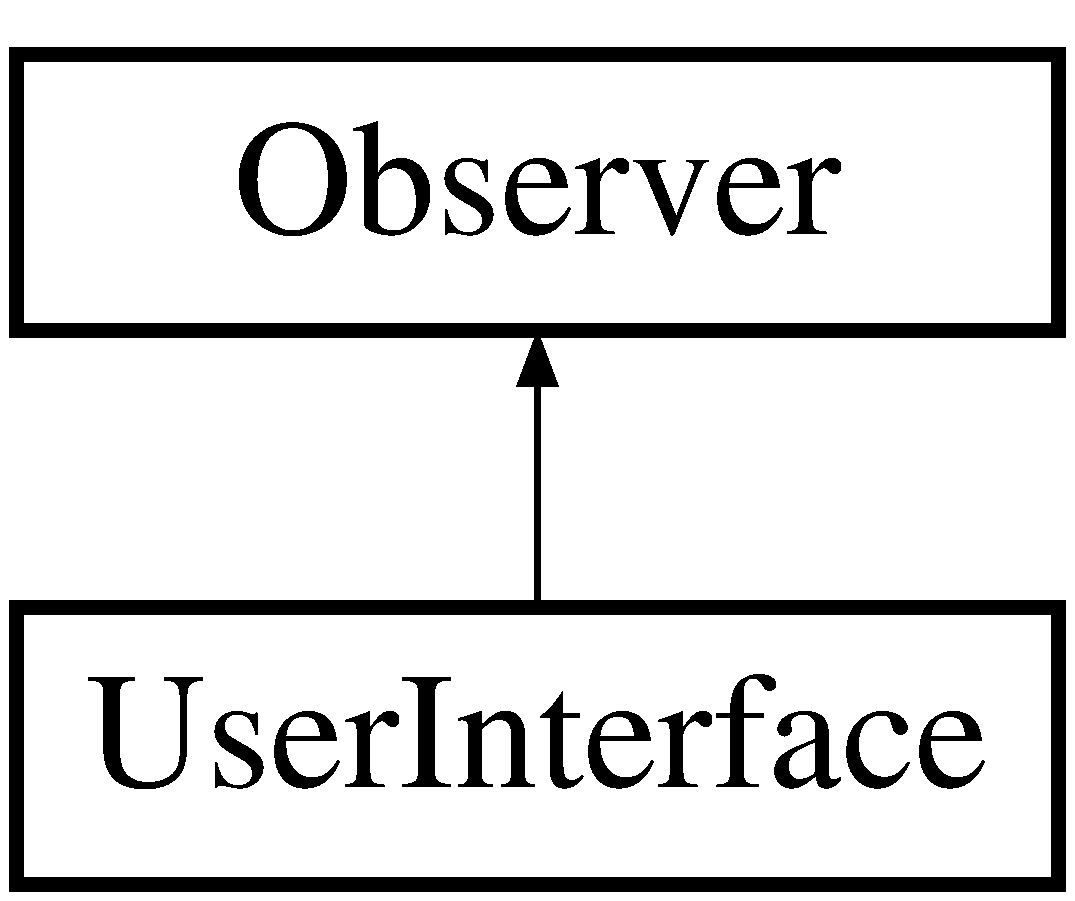
\includegraphics[height=2.000000cm]{class_observer}
\end{center}
\end{figure}
\subsection*{Public Member Functions}
\begin{DoxyCompactItemize}
\item 
virtual \hyperlink{class_observer_afcc6b67be6c386f2f3d2c363aa59cb47}{$\sim$\-Observer} ()
\item 
virtual void \hyperlink{class_observer_a6ee3bd29c7e16ce4d5208f39f09776ba}{Update} (\hyperlink{class_operation}{Operation} $\ast$operation)=0
\end{DoxyCompactItemize}
\subsection*{Protected Member Functions}
\begin{DoxyCompactItemize}
\item 
\hyperlink{class_observer_a19c43f80a38a332a6f694783df3c9835}{Observer} ()
\end{DoxyCompactItemize}
\subsection*{Private Member Functions}
\begin{DoxyCompactItemize}
\item 
\hyperlink{class_observer_a602ac85aafab6c5684ca2cf6ef322ec1}{N\-O\-\_\-\-C\-L\-A\-S\-S\-\_\-\-C\-O\-P\-Y} (\hyperlink{class_observer}{Observer})
\end{DoxyCompactItemize}


\subsection{Constructor \& Destructor Documentation}
\index{Observer@{Observer}!Observer@{Observer}}
\index{Observer@{Observer}!Observer@{Observer}}
\subsubsection[{Observer}]{\setlength{\rightskip}{0pt plus 5cm}Observer\-::\-Observer (
\begin{DoxyParamCaption}
{}
\end{DoxyParamCaption}
)\hspace{0.3cm}{\ttfamily [inline]}, {\ttfamily [protected]}}\label{class_observer_a19c43f80a38a332a6f694783df3c9835}
\index{Observer@{Observer}!$\sim$\-Observer@{$\sim$\-Observer}}
\index{$\sim$\-Observer@{$\sim$\-Observer}!Observer@{Observer}}
\subsubsection[{$\sim$\-Observer}]{\setlength{\rightskip}{0pt plus 5cm}virtual Observer\-::$\sim$\-Observer (
\begin{DoxyParamCaption}
{}
\end{DoxyParamCaption}
)\hspace{0.3cm}{\ttfamily [inline]}, {\ttfamily [virtual]}}\label{class_observer_afcc6b67be6c386f2f3d2c363aa59cb47}


\subsection{Member Function Documentation}
\index{Observer@{Observer}!N\-O\-\_\-\-C\-L\-A\-S\-S\-\_\-\-C\-O\-P\-Y@{N\-O\-\_\-\-C\-L\-A\-S\-S\-\_\-\-C\-O\-P\-Y}}
\index{N\-O\-\_\-\-C\-L\-A\-S\-S\-\_\-\-C\-O\-P\-Y@{N\-O\-\_\-\-C\-L\-A\-S\-S\-\_\-\-C\-O\-P\-Y}!Observer@{Observer}}
\subsubsection[{N\-O\-\_\-\-C\-L\-A\-S\-S\-\_\-\-C\-O\-P\-Y}]{\setlength{\rightskip}{0pt plus 5cm}Observer\-::\-N\-O\-\_\-\-C\-L\-A\-S\-S\-\_\-\-C\-O\-P\-Y (
\begin{DoxyParamCaption}
\item[{{\bf Observer}}]{}
\end{DoxyParamCaption}
)\hspace{0.3cm}{\ttfamily [private]}}\label{class_observer_a602ac85aafab6c5684ca2cf6ef322ec1}
\index{Observer@{Observer}!Update@{Update}}
\index{Update@{Update}!Observer@{Observer}}
\subsubsection[{Update}]{\setlength{\rightskip}{0pt plus 5cm}virtual void Observer\-::\-Update (
\begin{DoxyParamCaption}
\item[{{\bf Operation} $\ast$}]{operation}
\end{DoxyParamCaption}
)\hspace{0.3cm}{\ttfamily [pure virtual]}}\label{class_observer_a6ee3bd29c7e16ce4d5208f39f09776ba}


Implemented in \hyperlink{class_user_interface_a7f7df3c3de8a100dcadacb6bc4956302}{User\-Interface}.


\section{Operation Class Reference}
\label{class_operation}\index{Operation@{Operation}}


{\ttfamily \#include $<$Operation.\-h$>$}

\subsection*{Public Member Functions}
\begin{DoxyCompactItemize}
\item 
\hyperlink{class_operation_a55f76bcb8990f4dba577990af0c8399e}{Operation} ()
\item 
\hyperlink{class_operation_a14089623bd8a73e73375353c3d8a4b6e}{$\sim$\-Operation} ()
\item 
\hyperlink{_operation_8h_a29c331c24eda38b81f1e27a40391a589}{E\-\_\-\-O\-P\-E\-R\-A\-T\-I\-O\-N} \hyperlink{class_operation_ac848512e0fc5b66f1911bf2bfc17b56d}{Get\-Operation} () const 
\item 
std\-::string \hyperlink{class_operation_ace4ea581702ce225b0e2a89608100312}{Get\-Data} () const 
\item 
\hyperlink{structextra__data}{extra\-\_\-data} $\ast$ \hyperlink{class_operation_ae19cf9a5663925c03a897ae6177a43b4}{Get\-Extra\-Data} ()
\item 
D\-W\-O\-R\-D \hyperlink{class_operation_a75e5df9dbc5985f4b82bab9193378e6b}{Get\-Error\-Code} () const 
\item 
std\-::string \hyperlink{class_operation_aef57319b4837807d1d4c30c6ed53f814}{Get\-Error\-Msg} () const 
\item 
bool \hyperlink{class_operation_afca1d8978bb74555f0a6012d0984c90e}{Get\-Success} () const 
\item 
bool \hyperlink{class_operation_afbca526e90ce2af4bbc71817add9867d}{Has\-Executed} () const 
\item 
bool \hyperlink{class_operation_ab956c9ec646f7236607b21208e80a93c}{Is\-Prepared} () const 
\item 
bool \hyperlink{class_operation_abbe71fc5a2f6ef31a8ffd75685c2bc9e}{Is\-Paused} () const 
\item 
bool \hyperlink{class_operation_a0a609b1874688da41197d24ead40b5b6}{Was\-Needed} () const 
\item 
\hyperlink{class_operation}{Operation} $\ast$ \hyperlink{class_operation_a7704d1a6eb8321f2784551bb09f8daff}{Finished} (bool was\-\_\-needed=true)
\item 
\hyperlink{class_operation}{Operation} $\ast$ \hyperlink{class_operation_adbb06f3fb4fba2213530e1d544731165}{Had\-Error} (D\-W\-O\-R\-D err\-\_\-code, std\-::string err\-\_\-msg)
\item 
\hyperlink{class_operation}{Operation} $\ast$ \hyperlink{class_operation_ad72a4baf1246a151c3a96ee50f7ea4f7}{Pause} ()
\item 
\hyperlink{class_operation}{Operation} $\ast$ \hyperlink{class_operation_a9cf09be1677eb47538ace38ceb8d3fcb}{Prepare} (\hyperlink{_operation_8h_a29c331c24eda38b81f1e27a40391a589}{E\-\_\-\-O\-P\-E\-R\-A\-T\-I\-O\-N} operation, char $\ast$data\-\_\-format,...)
\item 
\hyperlink{class_operation}{Operation} $\ast$ \hyperlink{class_operation_ab8c5e5b425314aacb2c9ff4bbc4aead3}{Resume} ()
\end{DoxyCompactItemize}
\subsection*{Private Member Functions}
\begin{DoxyCompactItemize}
\item 
\hyperlink{class_operation_a944923ea5cc5043cb6223da880d7bfcc}{N\-O\-\_\-\-C\-L\-A\-S\-S\-\_\-\-A\-S\-S\-I\-G\-N\-M\-E\-N\-T} (\hyperlink{class_operation}{Operation})
\item 
\hyperlink{class_operation_a3628710ccd25dcc0fbd628d5234bd874}{N\-O\-\_\-\-C\-L\-A\-S\-S\-\_\-\-C\-O\-P\-Y} (\hyperlink{class_operation}{Operation})
\end{DoxyCompactItemize}
\subsection*{Private Attributes}
\begin{DoxyCompactItemize}
\item 
\hyperlink{_operation_8h_a29c331c24eda38b81f1e27a40391a589}{E\-\_\-\-O\-P\-E\-R\-A\-T\-I\-O\-N} \hyperlink{class_operation_ad78d85f09c55913fe1f82a0f77a0dc8c}{\-\_\-operation}
\item 
std\-::string \hyperlink{class_operation_a383d54b86fa3d166b491bcc82d1ce266}{\-\_\-data}
\item 
\hyperlink{structextra__data}{extra\-\_\-data} \hyperlink{class_operation_a1e970bd91884353e9bcb147ca27ecfa0}{\-\_\-extra\-\_\-data}
\item 
D\-W\-O\-R\-D \hyperlink{class_operation_a64908392b807de489bf0913eab33f859}{\-\_\-err\-\_\-code}
\item 
std\-::string \hyperlink{class_operation_aa1233375b7028c9870788468b8adf749}{\-\_\-err\-\_\-msg}
\item 
\hyperlink{_operation_8h_ac3f77f49db5f357de93e5a22bc2f601f}{E\-\_\-\-O\-P\-E\-R\-A\-T\-I\-O\-N\-\_\-\-S\-T\-A\-T\-E} \hyperlink{class_operation_afcd7896bcf67fa412e1af85cbb6d6b6b}{\-\_\-op\-\_\-state}
\end{DoxyCompactItemize}


\subsection{Detailed Description}
The functions return a pointer to the operation itself, so it can be used as a one-\/liner in a call to Notify(). 

\subsection{Constructor \& Destructor Documentation}
\index{Operation@{Operation}!Operation@{Operation}}
\index{Operation@{Operation}!Operation@{Operation}}
\subsubsection[{Operation}]{\setlength{\rightskip}{0pt plus 5cm}Operation\-::\-Operation (
\begin{DoxyParamCaption}
{}
\end{DoxyParamCaption}
)\hspace{0.3cm}{\ttfamily [inline]}}\label{class_operation_a55f76bcb8990f4dba577990af0c8399e}
\index{Operation@{Operation}!$\sim$\-Operation@{$\sim$\-Operation}}
\index{$\sim$\-Operation@{$\sim$\-Operation}!Operation@{Operation}}
\subsubsection[{$\sim$\-Operation}]{\setlength{\rightskip}{0pt plus 5cm}Operation\-::$\sim$\-Operation (
\begin{DoxyParamCaption}
{}
\end{DoxyParamCaption}
)\hspace{0.3cm}{\ttfamily [inline]}}\label{class_operation_a14089623bd8a73e73375353c3d8a4b6e}


\subsection{Member Function Documentation}
\index{Operation@{Operation}!Finished@{Finished}}
\index{Finished@{Finished}!Operation@{Operation}}
\subsubsection[{Finished}]{\setlength{\rightskip}{0pt plus 5cm}{\bf Operation} $\ast$ Operation\-::\-Finished (
\begin{DoxyParamCaption}
\item[{bool}]{was\-\_\-needed = {\ttfamily true}}
\end{DoxyParamCaption}
)}\label{class_operation_a7704d1a6eb8321f2784551bb09f8daff}
Completes the operation successfully.


\begin{DoxyParams}[1]{Parameters}
\mbox{\tt in}  & {\em was\-\_\-needed} & Flag if the operation was actually required; if a file doesn't exist for example, this is set to false, as it was marked to do, but was never found. Can be expanded to incorporate passing it to the notification, so it doesn't output to the U\-I. \\
\hline
\end{DoxyParams}
\begin{DoxyReturn}{Returns}
the pointer to the operation 
\end{DoxyReturn}
\index{Operation@{Operation}!Get\-Data@{Get\-Data}}
\index{Get\-Data@{Get\-Data}!Operation@{Operation}}
\subsubsection[{Get\-Data}]{\setlength{\rightskip}{0pt plus 5cm}std\-::string Operation\-::\-Get\-Data (
\begin{DoxyParamCaption}
{}
\end{DoxyParamCaption}
) const\hspace{0.3cm}{\ttfamily [inline]}}\label{class_operation_ace4ea581702ce225b0e2a89608100312}
\index{Operation@{Operation}!Get\-Error\-Code@{Get\-Error\-Code}}
\index{Get\-Error\-Code@{Get\-Error\-Code}!Operation@{Operation}}
\subsubsection[{Get\-Error\-Code}]{\setlength{\rightskip}{0pt plus 5cm}D\-W\-O\-R\-D Operation\-::\-Get\-Error\-Code (
\begin{DoxyParamCaption}
{}
\end{DoxyParamCaption}
) const\hspace{0.3cm}{\ttfamily [inline]}}\label{class_operation_a75e5df9dbc5985f4b82bab9193378e6b}
\index{Operation@{Operation}!Get\-Error\-Msg@{Get\-Error\-Msg}}
\index{Get\-Error\-Msg@{Get\-Error\-Msg}!Operation@{Operation}}
\subsubsection[{Get\-Error\-Msg}]{\setlength{\rightskip}{0pt plus 5cm}std\-::string Operation\-::\-Get\-Error\-Msg (
\begin{DoxyParamCaption}
{}
\end{DoxyParamCaption}
) const\hspace{0.3cm}{\ttfamily [inline]}}\label{class_operation_aef57319b4837807d1d4c30c6ed53f814}
\index{Operation@{Operation}!Get\-Extra\-Data@{Get\-Extra\-Data}}
\index{Get\-Extra\-Data@{Get\-Extra\-Data}!Operation@{Operation}}
\subsubsection[{Get\-Extra\-Data}]{\setlength{\rightskip}{0pt plus 5cm}{\bf extra\-\_\-data}$\ast$ Operation\-::\-Get\-Extra\-Data (
\begin{DoxyParamCaption}
{}
\end{DoxyParamCaption}
)\hspace{0.3cm}{\ttfamily [inline]}}\label{class_operation_ae19cf9a5663925c03a897ae6177a43b4}
\index{Operation@{Operation}!Get\-Operation@{Get\-Operation}}
\index{Get\-Operation@{Get\-Operation}!Operation@{Operation}}
\subsubsection[{Get\-Operation}]{\setlength{\rightskip}{0pt plus 5cm}{\bf E\-\_\-\-O\-P\-E\-R\-A\-T\-I\-O\-N} Operation\-::\-Get\-Operation (
\begin{DoxyParamCaption}
{}
\end{DoxyParamCaption}
) const\hspace{0.3cm}{\ttfamily [inline]}}\label{class_operation_ac848512e0fc5b66f1911bf2bfc17b56d}
\index{Operation@{Operation}!Get\-Success@{Get\-Success}}
\index{Get\-Success@{Get\-Success}!Operation@{Operation}}
\subsubsection[{Get\-Success}]{\setlength{\rightskip}{0pt plus 5cm}bool Operation\-::\-Get\-Success (
\begin{DoxyParamCaption}
{}
\end{DoxyParamCaption}
) const\hspace{0.3cm}{\ttfamily [inline]}}\label{class_operation_afca1d8978bb74555f0a6012d0984c90e}
\index{Operation@{Operation}!Had\-Error@{Had\-Error}}
\index{Had\-Error@{Had\-Error}!Operation@{Operation}}
\subsubsection[{Had\-Error}]{\setlength{\rightskip}{0pt plus 5cm}{\bf Operation} $\ast$ Operation\-::\-Had\-Error (
\begin{DoxyParamCaption}
\item[{D\-W\-O\-R\-D}]{err\-\_\-code, }
\item[{std\-::string}]{err\-\_\-msg}
\end{DoxyParamCaption}
)}\label{class_operation_adbb06f3fb4fba2213530e1d544731165}
Completes the operation, marking it as failed in execution.


\begin{DoxyParams}[1]{Parameters}
\mbox{\tt in}  & {\em err\-\_\-code} & The error code \\
\hline
\mbox{\tt in}  & {\em err\-\_\-msg} & The error message for the code \\
\hline
\end{DoxyParams}
\begin{DoxyReturn}{Returns}
the pointer to the operation 
\end{DoxyReturn}
\index{Operation@{Operation}!Has\-Executed@{Has\-Executed}}
\index{Has\-Executed@{Has\-Executed}!Operation@{Operation}}
\subsubsection[{Has\-Executed}]{\setlength{\rightskip}{0pt plus 5cm}bool Operation\-::\-Has\-Executed (
\begin{DoxyParamCaption}
{}
\end{DoxyParamCaption}
) const\hspace{0.3cm}{\ttfamily [inline]}}\label{class_operation_afbca526e90ce2af4bbc71817add9867d}
\index{Operation@{Operation}!Is\-Paused@{Is\-Paused}}
\index{Is\-Paused@{Is\-Paused}!Operation@{Operation}}
\subsubsection[{Is\-Paused}]{\setlength{\rightskip}{0pt plus 5cm}bool Operation\-::\-Is\-Paused (
\begin{DoxyParamCaption}
{}
\end{DoxyParamCaption}
) const\hspace{0.3cm}{\ttfamily [inline]}}\label{class_operation_abbe71fc5a2f6ef31a8ffd75685c2bc9e}
\index{Operation@{Operation}!Is\-Prepared@{Is\-Prepared}}
\index{Is\-Prepared@{Is\-Prepared}!Operation@{Operation}}
\subsubsection[{Is\-Prepared}]{\setlength{\rightskip}{0pt plus 5cm}bool Operation\-::\-Is\-Prepared (
\begin{DoxyParamCaption}
{}
\end{DoxyParamCaption}
) const\hspace{0.3cm}{\ttfamily [inline]}}\label{class_operation_ab956c9ec646f7236607b21208e80a93c}
\index{Operation@{Operation}!N\-O\-\_\-\-C\-L\-A\-S\-S\-\_\-\-A\-S\-S\-I\-G\-N\-M\-E\-N\-T@{N\-O\-\_\-\-C\-L\-A\-S\-S\-\_\-\-A\-S\-S\-I\-G\-N\-M\-E\-N\-T}}
\index{N\-O\-\_\-\-C\-L\-A\-S\-S\-\_\-\-A\-S\-S\-I\-G\-N\-M\-E\-N\-T@{N\-O\-\_\-\-C\-L\-A\-S\-S\-\_\-\-A\-S\-S\-I\-G\-N\-M\-E\-N\-T}!Operation@{Operation}}
\subsubsection[{N\-O\-\_\-\-C\-L\-A\-S\-S\-\_\-\-A\-S\-S\-I\-G\-N\-M\-E\-N\-T}]{\setlength{\rightskip}{0pt plus 5cm}Operation\-::\-N\-O\-\_\-\-C\-L\-A\-S\-S\-\_\-\-A\-S\-S\-I\-G\-N\-M\-E\-N\-T (
\begin{DoxyParamCaption}
\item[{{\bf Operation}}]{}
\end{DoxyParamCaption}
)\hspace{0.3cm}{\ttfamily [private]}}\label{class_operation_a944923ea5cc5043cb6223da880d7bfcc}
\index{Operation@{Operation}!N\-O\-\_\-\-C\-L\-A\-S\-S\-\_\-\-C\-O\-P\-Y@{N\-O\-\_\-\-C\-L\-A\-S\-S\-\_\-\-C\-O\-P\-Y}}
\index{N\-O\-\_\-\-C\-L\-A\-S\-S\-\_\-\-C\-O\-P\-Y@{N\-O\-\_\-\-C\-L\-A\-S\-S\-\_\-\-C\-O\-P\-Y}!Operation@{Operation}}
\subsubsection[{N\-O\-\_\-\-C\-L\-A\-S\-S\-\_\-\-C\-O\-P\-Y}]{\setlength{\rightskip}{0pt plus 5cm}Operation\-::\-N\-O\-\_\-\-C\-L\-A\-S\-S\-\_\-\-C\-O\-P\-Y (
\begin{DoxyParamCaption}
\item[{{\bf Operation}}]{}
\end{DoxyParamCaption}
)\hspace{0.3cm}{\ttfamily [private]}}\label{class_operation_a3628710ccd25dcc0fbd628d5234bd874}
\index{Operation@{Operation}!Pause@{Pause}}
\index{Pause@{Pause}!Operation@{Operation}}
\subsubsection[{Pause}]{\setlength{\rightskip}{0pt plus 5cm}{\bf Operation} $\ast$ Operation\-::\-Pause (
\begin{DoxyParamCaption}
{}
\end{DoxyParamCaption}
)}\label{class_operation_ad72a4baf1246a151c3a96ee50f7ea4f7}
Pauses the operation, usually when another operation is required in order for this one to succeed (usually in recursive folder deletes).

This is needed for the U\-I to be notified, so that it can drop down to a new line (as this one can't report completion or failure yet).

\begin{DoxyReturn}{Returns}
the pointer to the operation 
\end{DoxyReturn}
\index{Operation@{Operation}!Prepare@{Prepare}}
\index{Prepare@{Prepare}!Operation@{Operation}}
\subsubsection[{Prepare}]{\setlength{\rightskip}{0pt plus 5cm}{\bf Operation} $\ast$ Operation\-::\-Prepare (
\begin{DoxyParamCaption}
\item[{{\bf E\-\_\-\-O\-P\-E\-R\-A\-T\-I\-O\-N}}]{operation, }
\item[{char $\ast$}]{data\-\_\-format, }
\item[{}]{...}
\end{DoxyParamCaption}
)}\label{class_operation_a9cf09be1677eb47538ace38ceb8d3fcb}
Generates the textual output to put to the screen, and also depending on the operation, sets the data for it (i.\-e. the data format will be the path to a file if the operation is O\-P\-\_\-\-Delete\-File, and so on).


\begin{DoxyParams}[1]{Parameters}
\mbox{\tt in}  & {\em operation} & The type of operation to perform \\
\hline
\mbox{\tt in}  & {\em data\-\_\-format} & The format-\/string of the parameters to use as the input data \\
\hline
\mbox{\tt in}  & {\em ...} & The rest of the parameters as required by the format\\
\hline
\end{DoxyParams}
\begin{DoxyReturn}{Returns}
the pointer to the operation 
\end{DoxyReturn}
\index{Operation@{Operation}!Resume@{Resume}}
\index{Resume@{Resume}!Operation@{Operation}}
\subsubsection[{Resume}]{\setlength{\rightskip}{0pt plus 5cm}{\bf Operation} $\ast$ Operation\-::\-Resume (
\begin{DoxyParamCaption}
{}
\end{DoxyParamCaption}
)}\label{class_operation_ab8c5e5b425314aacb2c9ff4bbc4aead3}
Resumes the operation after a prior \hyperlink{class_operation_ad72a4baf1246a151c3a96ee50f7ea4f7}{Pause()}.

\begin{DoxyReturn}{Returns}
the pointer to the operation 
\end{DoxyReturn}
\index{Operation@{Operation}!Was\-Needed@{Was\-Needed}}
\index{Was\-Needed@{Was\-Needed}!Operation@{Operation}}
\subsubsection[{Was\-Needed}]{\setlength{\rightskip}{0pt plus 5cm}bool Operation\-::\-Was\-Needed (
\begin{DoxyParamCaption}
{}
\end{DoxyParamCaption}
) const\hspace{0.3cm}{\ttfamily [inline]}}\label{class_operation_a0a609b1874688da41197d24ead40b5b6}


\subsection{Member Data Documentation}
\index{Operation@{Operation}!\-\_\-data@{\-\_\-data}}
\index{\-\_\-data@{\-\_\-data}!Operation@{Operation}}
\subsubsection[{\-\_\-data}]{\setlength{\rightskip}{0pt plus 5cm}std\-::string Operation\-::\-\_\-data\hspace{0.3cm}{\ttfamily [private]}}\label{class_operation_a383d54b86fa3d166b491bcc82d1ce266}
\index{Operation@{Operation}!\-\_\-err\-\_\-code@{\-\_\-err\-\_\-code}}
\index{\-\_\-err\-\_\-code@{\-\_\-err\-\_\-code}!Operation@{Operation}}
\subsubsection[{\-\_\-err\-\_\-code}]{\setlength{\rightskip}{0pt plus 5cm}D\-W\-O\-R\-D Operation\-::\-\_\-err\-\_\-code\hspace{0.3cm}{\ttfamily [private]}}\label{class_operation_a64908392b807de489bf0913eab33f859}
\index{Operation@{Operation}!\-\_\-err\-\_\-msg@{\-\_\-err\-\_\-msg}}
\index{\-\_\-err\-\_\-msg@{\-\_\-err\-\_\-msg}!Operation@{Operation}}
\subsubsection[{\-\_\-err\-\_\-msg}]{\setlength{\rightskip}{0pt plus 5cm}std\-::string Operation\-::\-\_\-err\-\_\-msg\hspace{0.3cm}{\ttfamily [private]}}\label{class_operation_aa1233375b7028c9870788468b8adf749}
\index{Operation@{Operation}!\-\_\-extra\-\_\-data@{\-\_\-extra\-\_\-data}}
\index{\-\_\-extra\-\_\-data@{\-\_\-extra\-\_\-data}!Operation@{Operation}}
\subsubsection[{\-\_\-extra\-\_\-data}]{\setlength{\rightskip}{0pt plus 5cm}{\bf extra\-\_\-data} Operation\-::\-\_\-extra\-\_\-data\hspace{0.3cm}{\ttfamily [private]}}\label{class_operation_a1e970bd91884353e9bcb147ca27ecfa0}
\index{Operation@{Operation}!\-\_\-op\-\_\-state@{\-\_\-op\-\_\-state}}
\index{\-\_\-op\-\_\-state@{\-\_\-op\-\_\-state}!Operation@{Operation}}
\subsubsection[{\-\_\-op\-\_\-state}]{\setlength{\rightskip}{0pt plus 5cm}{\bf E\-\_\-\-O\-P\-E\-R\-A\-T\-I\-O\-N\-\_\-\-S\-T\-A\-T\-E} Operation\-::\-\_\-op\-\_\-state\hspace{0.3cm}{\ttfamily [private]}}\label{class_operation_afcd7896bcf67fa412e1af85cbb6d6b6b}
\index{Operation@{Operation}!\-\_\-operation@{\-\_\-operation}}
\index{\-\_\-operation@{\-\_\-operation}!Operation@{Operation}}
\subsubsection[{\-\_\-operation}]{\setlength{\rightskip}{0pt plus 5cm}{\bf E\-\_\-\-O\-P\-E\-R\-A\-T\-I\-O\-N} Operation\-::\-\_\-operation\hspace{0.3cm}{\ttfamily [private]}}\label{class_operation_ad78d85f09c55913fe1f82a0f77a0dc8c}

\section{Configuration\-:\-:proxy$<$ T $>$ Class Template Reference}
\label{class_configuration_1_1proxy}\index{Configuration\-::proxy$<$ T $>$@{Configuration\-::proxy$<$ T $>$}}


{\ttfamily \#include $<$Configuration.\-h$>$}

\subsection*{Public Member Functions}
\begin{DoxyCompactItemize}
\item 
\hyperlink{class_configuration_1_1proxy_ab4337c85e11d9a259e394590c07a5fe4}{proxy} ()
\item 
\hyperlink{class_configuration_1_1proxy_a38a07083e576ba14cabfc23461e8c089}{operator const T \&} () const 
\item 
\hyperlink{class_configuration_1_1proxy_a631982c73c73189824f209c1178cff2d}{operator const T \&} ()
\end{DoxyCompactItemize}
\subsection*{Private Member Functions}
\begin{DoxyCompactItemize}
\item 
T \hyperlink{class_configuration_1_1proxy_a80e382c028406f4599ef088f0d64849b}{operator=} (const T \&arg)
\end{DoxyCompactItemize}
\subsection*{Private Attributes}
\begin{DoxyCompactItemize}
\item 
T \hyperlink{class_configuration_1_1proxy_aeff1982d30095641c59ada398672b8e1}{data}
\end{DoxyCompactItemize}
\subsection*{Friends}
\begin{DoxyCompactItemize}
\item 
class \hyperlink{class_configuration_1_1proxy_a30221ddc558692a7b52598b963a74bc2}{Configuration}
\item 
bool \hyperlink{class_configuration_1_1proxy_a77d8ecb3e2084eecf8db1cf62276bcf0}{parse\-\_\-commandline} (\hyperlink{stdint_8h_a32f2e37ee053cf2ce8ca28d1f74630e5}{int32\-\_\-t} argc, char $\ast$$\ast$argv)
\end{DoxyCompactItemize}


\subsection{Constructor \& Destructor Documentation}
\index{Configuration\-::proxy@{Configuration\-::proxy}!proxy@{proxy}}
\index{proxy@{proxy}!Configuration::proxy@{Configuration\-::proxy}}
\subsubsection[{proxy}]{\setlength{\rightskip}{0pt plus 5cm}template$<$class T$>$ {\bf Configuration\-::proxy}$<$ T $>$\-::{\bf proxy} (
\begin{DoxyParamCaption}
{}
\end{DoxyParamCaption}
)\hspace{0.3cm}{\ttfamily [inline]}}\label{class_configuration_1_1proxy_ab4337c85e11d9a259e394590c07a5fe4}


\subsection{Member Function Documentation}
\index{Configuration\-::proxy@{Configuration\-::proxy}!operator const T \&@{operator const T \&}}
\index{operator const T \&@{operator const T \&}!Configuration::proxy@{Configuration\-::proxy}}
\subsubsection[{operator const T \&}]{\setlength{\rightskip}{0pt plus 5cm}template$<$class T$>$ {\bf Configuration\-::proxy}$<$ T $>$\-::operator const T \& (
\begin{DoxyParamCaption}
{}
\end{DoxyParamCaption}
) const\hspace{0.3cm}{\ttfamily [inline]}}\label{class_configuration_1_1proxy_a38a07083e576ba14cabfc23461e8c089}
\index{Configuration\-::proxy@{Configuration\-::proxy}!operator const T \&@{operator const T \&}}
\index{operator const T \&@{operator const T \&}!Configuration::proxy@{Configuration\-::proxy}}
\subsubsection[{operator const T \&}]{\setlength{\rightskip}{0pt plus 5cm}template$<$class T$>$ {\bf Configuration\-::proxy}$<$ T $>$\-::operator const T \& (
\begin{DoxyParamCaption}
{}
\end{DoxyParamCaption}
)\hspace{0.3cm}{\ttfamily [inline]}}\label{class_configuration_1_1proxy_a631982c73c73189824f209c1178cff2d}
\index{Configuration\-::proxy@{Configuration\-::proxy}!operator=@{operator=}}
\index{operator=@{operator=}!Configuration::proxy@{Configuration\-::proxy}}
\subsubsection[{operator=}]{\setlength{\rightskip}{0pt plus 5cm}template$<$class T$>$ T {\bf Configuration\-::proxy}$<$ T $>$\-::operator= (
\begin{DoxyParamCaption}
\item[{const T \&}]{arg}
\end{DoxyParamCaption}
)\hspace{0.3cm}{\ttfamily [inline]}, {\ttfamily [private]}}\label{class_configuration_1_1proxy_a80e382c028406f4599ef088f0d64849b}


\subsection{Friends And Related Function Documentation}
\index{Configuration\-::proxy@{Configuration\-::proxy}!Configuration@{Configuration}}
\index{Configuration@{Configuration}!Configuration::proxy@{Configuration\-::proxy}}
\subsubsection[{Configuration}]{\setlength{\rightskip}{0pt plus 5cm}template$<$class T$>$ friend class {\bf Configuration}\hspace{0.3cm}{\ttfamily [friend]}}\label{class_configuration_1_1proxy_a30221ddc558692a7b52598b963a74bc2}
\index{Configuration\-::proxy@{Configuration\-::proxy}!parse\-\_\-commandline@{parse\-\_\-commandline}}
\index{parse\-\_\-commandline@{parse\-\_\-commandline}!Configuration::proxy@{Configuration\-::proxy}}
\subsubsection[{parse\-\_\-commandline}]{\setlength{\rightskip}{0pt plus 5cm}template$<$class T$>$ bool parse\-\_\-commandline (
\begin{DoxyParamCaption}
\item[{{\bf int32\-\_\-t}}]{argc, }
\item[{char $\ast$$\ast$}]{argv}
\end{DoxyParamCaption}
)\hspace{0.3cm}{\ttfamily [friend]}}\label{class_configuration_1_1proxy_a77d8ecb3e2084eecf8db1cf62276bcf0}
Parses the application command line, setting runtime configuration options. Separate function from the \hyperlink{class_configuration}{Configuration} as it should only be executed once, and within \hyperlink{app_8cc_a7ab0624f9c8aeab843f91432c75638ee}{app\-\_\-init()}, where the parameters are available.


\begin{DoxyParams}{Parameters}
{\em argc} & The number of arguments passed in \\
\hline
{\em argv} & An array of pointers to the arguments \\
\hline
\end{DoxyParams}
\begin{DoxyReturn}{Returns}
true is returned if any and all command line options are processed successfully 

false is only returned if an unknown parameter is provided, or an invalid option is passed to a parameter 
\end{DoxyReturn}


\subsection{Member Data Documentation}
\index{Configuration\-::proxy@{Configuration\-::proxy}!data@{data}}
\index{data@{data}!Configuration::proxy@{Configuration\-::proxy}}
\subsubsection[{data}]{\setlength{\rightskip}{0pt plus 5cm}template$<$class T$>$ T {\bf Configuration\-::proxy}$<$ T $>$\-::data\hspace{0.3cm}{\ttfamily [private]}}\label{class_configuration_1_1proxy_aeff1982d30095641c59ada398672b8e1}

\section{User\-Interface\-:\-:proxy$<$ T $>$ Class Template Reference}
\label{class_user_interface_1_1proxy}\index{User\-Interface\-::proxy$<$ T $>$@{User\-Interface\-::proxy$<$ T $>$}}


{\ttfamily \#include $<$User\-Interface.\-h$>$}

\subsection*{Public Member Functions}
\begin{DoxyCompactItemize}
\item 
\hyperlink{class_user_interface_1_1proxy_a1a192470532b54f2a474a9b2caad8d49}{proxy} ()
\item 
\hyperlink{class_user_interface_1_1proxy_ac7a983433d3dd29017a45188338c21b1}{operator const T \&} () const 
\item 
\hyperlink{class_user_interface_1_1proxy_a5e3cad4ce73f0a0281d1655b9ca6f841}{operator const T \&} ()
\end{DoxyCompactItemize}
\subsection*{Private Member Functions}
\begin{DoxyCompactItemize}
\item 
T \hyperlink{class_user_interface_1_1proxy_a01e55fd178489fc3b2e4c4c82199cd30}{operator=} (const T \&arg)
\end{DoxyCompactItemize}
\subsection*{Private Attributes}
\begin{DoxyCompactItemize}
\item 
T \hyperlink{class_user_interface_1_1proxy_a5f38ae21b583b9419bd65bd11b426f36}{data}
\end{DoxyCompactItemize}
\subsection*{Friends}
\begin{DoxyCompactItemize}
\item 
class \hyperlink{class_user_interface_1_1proxy_adb55a5cf0f8d4b17f324a902a7904d97}{User\-Interface}
\item 
void \hyperlink{class_user_interface_1_1proxy_a7ab0624f9c8aeab843f91432c75638ee}{app\-\_\-init} (\hyperlink{stdint_8h_a32f2e37ee053cf2ce8ca28d1f74630e5}{int32\-\_\-t} argc, char $\ast$$\ast$argv)
\item 
void \hyperlink{class_user_interface_1_1proxy_a6d05bd04f7411a8f5441f0f1a7221225}{app\-\_\-free} ()
\end{DoxyCompactItemize}


\subsection{Constructor \& Destructor Documentation}
\index{User\-Interface\-::proxy@{User\-Interface\-::proxy}!proxy@{proxy}}
\index{proxy@{proxy}!UserInterface::proxy@{User\-Interface\-::proxy}}
\subsubsection[{proxy}]{\setlength{\rightskip}{0pt plus 5cm}template$<$class T$>$ {\bf User\-Interface\-::proxy}$<$ T $>$\-::{\bf proxy} (
\begin{DoxyParamCaption}
{}
\end{DoxyParamCaption}
)\hspace{0.3cm}{\ttfamily [inline]}}\label{class_user_interface_1_1proxy_a1a192470532b54f2a474a9b2caad8d49}


\subsection{Member Function Documentation}
\index{User\-Interface\-::proxy@{User\-Interface\-::proxy}!operator const T \&@{operator const T \&}}
\index{operator const T \&@{operator const T \&}!UserInterface::proxy@{User\-Interface\-::proxy}}
\subsubsection[{operator const T \&}]{\setlength{\rightskip}{0pt plus 5cm}template$<$class T$>$ {\bf User\-Interface\-::proxy}$<$ T $>$\-::operator const T \& (
\begin{DoxyParamCaption}
{}
\end{DoxyParamCaption}
) const\hspace{0.3cm}{\ttfamily [inline]}}\label{class_user_interface_1_1proxy_ac7a983433d3dd29017a45188338c21b1}
\index{User\-Interface\-::proxy@{User\-Interface\-::proxy}!operator const T \&@{operator const T \&}}
\index{operator const T \&@{operator const T \&}!UserInterface::proxy@{User\-Interface\-::proxy}}
\subsubsection[{operator const T \&}]{\setlength{\rightskip}{0pt plus 5cm}template$<$class T$>$ {\bf User\-Interface\-::proxy}$<$ T $>$\-::operator const T \& (
\begin{DoxyParamCaption}
{}
\end{DoxyParamCaption}
)\hspace{0.3cm}{\ttfamily [inline]}}\label{class_user_interface_1_1proxy_a5e3cad4ce73f0a0281d1655b9ca6f841}
\index{User\-Interface\-::proxy@{User\-Interface\-::proxy}!operator=@{operator=}}
\index{operator=@{operator=}!UserInterface::proxy@{User\-Interface\-::proxy}}
\subsubsection[{operator=}]{\setlength{\rightskip}{0pt plus 5cm}template$<$class T$>$ T {\bf User\-Interface\-::proxy}$<$ T $>$\-::operator= (
\begin{DoxyParamCaption}
\item[{const T \&}]{arg}
\end{DoxyParamCaption}
)\hspace{0.3cm}{\ttfamily [inline]}, {\ttfamily [private]}}\label{class_user_interface_1_1proxy_a01e55fd178489fc3b2e4c4c82199cd30}


\subsection{Friends And Related Function Documentation}
\index{User\-Interface\-::proxy@{User\-Interface\-::proxy}!app\-\_\-free@{app\-\_\-free}}
\index{app\-\_\-free@{app\-\_\-free}!UserInterface::proxy@{User\-Interface\-::proxy}}
\subsubsection[{app\-\_\-free}]{\setlength{\rightskip}{0pt plus 5cm}template$<$class T$>$ void app\-\_\-free (
\begin{DoxyParamCaption}
{}
\end{DoxyParamCaption}
)\hspace{0.3cm}{\ttfamily [friend]}}\label{class_user_interface_1_1proxy_a6d05bd04f7411a8f5441f0f1a7221225}
\index{User\-Interface\-::proxy@{User\-Interface\-::proxy}!app\-\_\-init@{app\-\_\-init}}
\index{app\-\_\-init@{app\-\_\-init}!UserInterface::proxy@{User\-Interface\-::proxy}}
\subsubsection[{app\-\_\-init}]{\setlength{\rightskip}{0pt plus 5cm}template$<$class T$>$ void app\-\_\-init (
\begin{DoxyParamCaption}
\item[{{\bf int32\-\_\-t}}]{argc, }
\item[{char $\ast$$\ast$}]{argv}
\end{DoxyParamCaption}
)\hspace{0.3cm}{\ttfamily [friend]}}\label{class_user_interface_1_1proxy_a7ab0624f9c8aeab843f91432c75638ee}
Initializes the application; loads the configuration, handles the creation and movement of the windows, and prepares the windows if using a graphical configuration.

The static classes in \hyperlink{class_runtime}{Runtime} can be called safely once this function has completed, not before.

Receives the argc and argv passed in from \hyperlink{main_8cc_af19ddca125f05a2090dd132045573ee4}{main()} directly; if using the G\-U\-I, argc \& argv are acquired by a Visual Studio specific ability -\/ \-\_\-\-\_\-argc and \-\_\-\-\_\-argv. They contain the same data in the same way.


\begin{DoxyParams}[1]{Parameters}
\mbox{\tt in}  & {\em argc} & The number of command-\/line arguments supplied \\
\hline
\mbox{\tt in}  & {\em argv} & A pointer to an array of command-\/line arguments \\
\hline
\end{DoxyParams}
\begin{DoxyRefDesc}{Todo}
\item[\hyperlink{todo__todo000002}{Todo}]Add W\-S\-\_\-\-M\-A\-X\-I\-M\-I\-Z\-E\-B\-O\-X$|$\-W\-S\-\_\-\-M\-I\-N\-I\-M\-I\-Z\-E\-B\-O\-X$|$ and support a resizing window. Not critical to add at the current time. \end{DoxyRefDesc}
\index{User\-Interface\-::proxy@{User\-Interface\-::proxy}!User\-Interface@{User\-Interface}}
\index{User\-Interface@{User\-Interface}!UserInterface::proxy@{User\-Interface\-::proxy}}
\subsubsection[{User\-Interface}]{\setlength{\rightskip}{0pt plus 5cm}template$<$class T$>$ friend class {\bf User\-Interface}\hspace{0.3cm}{\ttfamily [friend]}}\label{class_user_interface_1_1proxy_adb55a5cf0f8d4b17f324a902a7904d97}


\subsection{Member Data Documentation}
\index{User\-Interface\-::proxy@{User\-Interface\-::proxy}!data@{data}}
\index{data@{data}!UserInterface::proxy@{User\-Interface\-::proxy}}
\subsubsection[{data}]{\setlength{\rightskip}{0pt plus 5cm}template$<$class T$>$ T {\bf User\-Interface\-::proxy}$<$ T $>$\-::data\hspace{0.3cm}{\ttfamily [private]}}\label{class_user_interface_1_1proxy_a5f38ae21b583b9419bd65bd11b426f36}

\section{Runtime Class Reference}
\label{class_runtime}\index{Runtime@{Runtime}}


{\ttfamily \#include $<$Runtime.\-h$>$}

\subsection*{Public Member Functions}
\begin{DoxyCompactItemize}
\item 
\hyperlink{class_configuration}{Configuration} $\ast$ \hyperlink{class_runtime_a42500720bee2cf4002c945b494a44ced}{Config} () const 
\item 
\hyperlink{class_log}{Log} $\ast$ \hyperlink{class_runtime_aa257050eab90cb6493b1cadcd003b67f}{Logger} () const 
\item 
\hyperlink{class_file_parser}{File\-Parser} $\ast$ \hyperlink{class_runtime_ae976465b16782d87ad46b836b63dfb00}{Parser} () const 
\item 
\hyperlink{class_user_interface}{User\-Interface} $\ast$ \hyperlink{class_runtime_ada47d441b13bc24accea9dca292eeced}{U\-I} () const 
\item 
\hyperlink{class_wiper}{Wiper} $\ast$ \hyperlink{class_runtime_a67e200aad11db275aba4230282ce6eae}{Wiper} () const 
\end{DoxyCompactItemize}
\subsection*{Static Public Member Functions}
\begin{DoxyCompactItemize}
\item 
static \hyperlink{class_runtime}{Runtime} \& \hyperlink{class_runtime_a1146c295df34dff8c1935ec0436edd7d}{Instance} ()
\end{DoxyCompactItemize}
\subsection*{Private Member Functions}
\begin{DoxyCompactItemize}
\item 
\hyperlink{class_runtime_a6a3920f0c4052fa28177f539b402d2e4}{N\-O\-\_\-\-C\-L\-A\-S\-S\-\_\-\-A\-S\-S\-I\-G\-N\-M\-E\-N\-T} (\hyperlink{class_runtime}{Runtime})
\item 
\hyperlink{class_runtime_a9b37cdb81eff355717a177408b5c180c}{N\-O\-\_\-\-C\-L\-A\-S\-S\-\_\-\-C\-O\-P\-Y} (\hyperlink{class_runtime}{Runtime})
\item 
\hyperlink{class_runtime_a522dc4b36f2a770bbe3e62c451f38841}{Runtime} ()
\item 
\hyperlink{class_runtime_a69418e2a8c03d0e24cdc63eb88b52d28}{$\sim$\-Runtime} ()
\end{DoxyCompactItemize}


\subsection{Detailed Description}
Dedicated class for storing all 'global' variables. This itself is accessed through an extern by the runtime code, so is in itself actually a global.

While this is a technical misuse of a Singleton, since there can only ever be one runtime (which we can then use to interface with the host O\-S and also maintains if the app is quitting, for example), it seems appropriate and can easily be replaced with the way it has been designed.

The classes accessed are not constructed until their first call, which keeps the application startup brief. You can therefore make assumptions in the child classes about the lifetimes of other objects, and safely know each will have their destructor called before the runtime is destroyed.

Yes, this can be implemented in other ways -\/ but this is clear and concise, without {\itshape too} many of the issues commonly associated with bad singleton use.

On Windows, this constructor is executed before \hyperlink{main_8cc_af19ddca125f05a2090dd132045573ee4}{main()} is entered; the actual call stack is (assuming Windows subsystem)\-: \begin{DoxyVerb}- Runtime()
- _initterm
- __tmainCRTStartup (also calls main)
- WinMainCRTStartup
\end{DoxyVerb}
 

\subsection{Constructor \& Destructor Documentation}
\index{Runtime@{Runtime}!Runtime@{Runtime}}
\index{Runtime@{Runtime}!Runtime@{Runtime}}
\subsubsection[{Runtime}]{\setlength{\rightskip}{0pt plus 5cm}Runtime\-::\-Runtime (
\begin{DoxyParamCaption}
{}
\end{DoxyParamCaption}
)\hspace{0.3cm}{\ttfamily [private]}}\label{class_runtime_a522dc4b36f2a770bbe3e62c451f38841}
\index{Runtime@{Runtime}!$\sim$\-Runtime@{$\sim$\-Runtime}}
\index{$\sim$\-Runtime@{$\sim$\-Runtime}!Runtime@{Runtime}}
\subsubsection[{$\sim$\-Runtime}]{\setlength{\rightskip}{0pt plus 5cm}Runtime\-::$\sim$\-Runtime (
\begin{DoxyParamCaption}
{}
\end{DoxyParamCaption}
)\hspace{0.3cm}{\ttfamily [private]}}\label{class_runtime_a69418e2a8c03d0e24cdc63eb88b52d28}


\subsection{Member Function Documentation}
\index{Runtime@{Runtime}!Config@{Config}}
\index{Config@{Config}!Runtime@{Runtime}}
\subsubsection[{Config}]{\setlength{\rightskip}{0pt plus 5cm}{\bf Configuration} $\ast$ Runtime\-::\-Config (
\begin{DoxyParamCaption}
{}
\end{DoxyParamCaption}
) const}\label{class_runtime_a42500720bee2cf4002c945b494a44ced}
Retrieves a pointer to the static \hyperlink{class_configuration}{Configuration} variable.

\begin{DoxyReturn}{Returns}
Always returns a pointer to a \hyperlink{class_configuration}{Configuration} instance; never fails 
\end{DoxyReturn}
\index{Runtime@{Runtime}!Instance@{Instance}}
\index{Instance@{Instance}!Runtime@{Runtime}}
\subsubsection[{Instance}]{\setlength{\rightskip}{0pt plus 5cm}static {\bf Runtime}\& Runtime\-::\-Instance (
\begin{DoxyParamCaption}
{}
\end{DoxyParamCaption}
)\hspace{0.3cm}{\ttfamily [inline]}, {\ttfamily [static]}}\label{class_runtime_a1146c295df34dff8c1935ec0436edd7d}
Acquires the singleton reference to the class. Only used within \hyperlink{app_8cc}{app.\-cc} in order to make the runtime accessible globally (accessed by 'runtime') -\/ shouldn't be used outside of this. \index{Runtime@{Runtime}!Logger@{Logger}}
\index{Logger@{Logger}!Runtime@{Runtime}}
\subsubsection[{Logger}]{\setlength{\rightskip}{0pt plus 5cm}{\bf Log} $\ast$ Runtime\-::\-Logger (
\begin{DoxyParamCaption}
{}
\end{DoxyParamCaption}
) const}\label{class_runtime_aa257050eab90cb6493b1cadcd003b67f}
Retrieves a pointer to the static \hyperlink{class_log}{Log} variable.

\begin{DoxyReturn}{Returns}
Always returns a pointer to a \hyperlink{class_log}{Log} instance; never fails 
\end{DoxyReturn}
\index{Runtime@{Runtime}!N\-O\-\_\-\-C\-L\-A\-S\-S\-\_\-\-A\-S\-S\-I\-G\-N\-M\-E\-N\-T@{N\-O\-\_\-\-C\-L\-A\-S\-S\-\_\-\-A\-S\-S\-I\-G\-N\-M\-E\-N\-T}}
\index{N\-O\-\_\-\-C\-L\-A\-S\-S\-\_\-\-A\-S\-S\-I\-G\-N\-M\-E\-N\-T@{N\-O\-\_\-\-C\-L\-A\-S\-S\-\_\-\-A\-S\-S\-I\-G\-N\-M\-E\-N\-T}!Runtime@{Runtime}}
\subsubsection[{N\-O\-\_\-\-C\-L\-A\-S\-S\-\_\-\-A\-S\-S\-I\-G\-N\-M\-E\-N\-T}]{\setlength{\rightskip}{0pt plus 5cm}Runtime\-::\-N\-O\-\_\-\-C\-L\-A\-S\-S\-\_\-\-A\-S\-S\-I\-G\-N\-M\-E\-N\-T (
\begin{DoxyParamCaption}
\item[{{\bf Runtime}}]{}
\end{DoxyParamCaption}
)\hspace{0.3cm}{\ttfamily [private]}}\label{class_runtime_a6a3920f0c4052fa28177f539b402d2e4}
\index{Runtime@{Runtime}!N\-O\-\_\-\-C\-L\-A\-S\-S\-\_\-\-C\-O\-P\-Y@{N\-O\-\_\-\-C\-L\-A\-S\-S\-\_\-\-C\-O\-P\-Y}}
\index{N\-O\-\_\-\-C\-L\-A\-S\-S\-\_\-\-C\-O\-P\-Y@{N\-O\-\_\-\-C\-L\-A\-S\-S\-\_\-\-C\-O\-P\-Y}!Runtime@{Runtime}}
\subsubsection[{N\-O\-\_\-\-C\-L\-A\-S\-S\-\_\-\-C\-O\-P\-Y}]{\setlength{\rightskip}{0pt plus 5cm}Runtime\-::\-N\-O\-\_\-\-C\-L\-A\-S\-S\-\_\-\-C\-O\-P\-Y (
\begin{DoxyParamCaption}
\item[{{\bf Runtime}}]{}
\end{DoxyParamCaption}
)\hspace{0.3cm}{\ttfamily [private]}}\label{class_runtime_a9b37cdb81eff355717a177408b5c180c}
\index{Runtime@{Runtime}!Parser@{Parser}}
\index{Parser@{Parser}!Runtime@{Runtime}}
\subsubsection[{Parser}]{\setlength{\rightskip}{0pt plus 5cm}{\bf File\-Parser} $\ast$ Runtime\-::\-Parser (
\begin{DoxyParamCaption}
{}
\end{DoxyParamCaption}
) const}\label{class_runtime_ae976465b16782d87ad46b836b63dfb00}
Retrieves a pointer to the static Parser variable.

\begin{DoxyReturn}{Returns}
Always returns a pointer to a Parser instance; never fails 
\end{DoxyReturn}
\index{Runtime@{Runtime}!U\-I@{U\-I}}
\index{U\-I@{U\-I}!Runtime@{Runtime}}
\subsubsection[{U\-I}]{\setlength{\rightskip}{0pt plus 5cm}{\bf User\-Interface} $\ast$ Runtime\-::\-U\-I (
\begin{DoxyParamCaption}
{}
\end{DoxyParamCaption}
) const}\label{class_runtime_ada47d441b13bc24accea9dca292eeced}
Retrieves a pointer to the static \hyperlink{class_user_interface}{User\-Interface} variable.

\begin{DoxyReturn}{Returns}
Always returns a pointer to a \hyperlink{class_user_interface}{User\-Interface} instance; never fails 
\end{DoxyReturn}
\index{Runtime@{Runtime}!Wiper@{Wiper}}
\index{Wiper@{Wiper}!Runtime@{Runtime}}
\subsubsection[{Wiper}]{\setlength{\rightskip}{0pt plus 5cm}{\bf Wiper} $\ast$ Runtime\-::\-Wiper (
\begin{DoxyParamCaption}
{}
\end{DoxyParamCaption}
) const}\label{class_runtime_a67e200aad11db275aba4230282ce6eae}
Retrieves a pointer to the static \hyperlink{class_wiper}{Wiper} variable.

\begin{DoxyReturn}{Returns}
Always returns a pointer to a \hyperlink{class_wiper}{Wiper} instance; never fails 
\end{DoxyReturn}

\section{Subject Class Reference}
\label{class_subject}\index{Subject@{Subject}}


{\ttfamily \#include $<$Subject.\-h$>$}

Inheritance diagram for Subject\-:\begin{figure}[H]
\begin{center}
\leavevmode
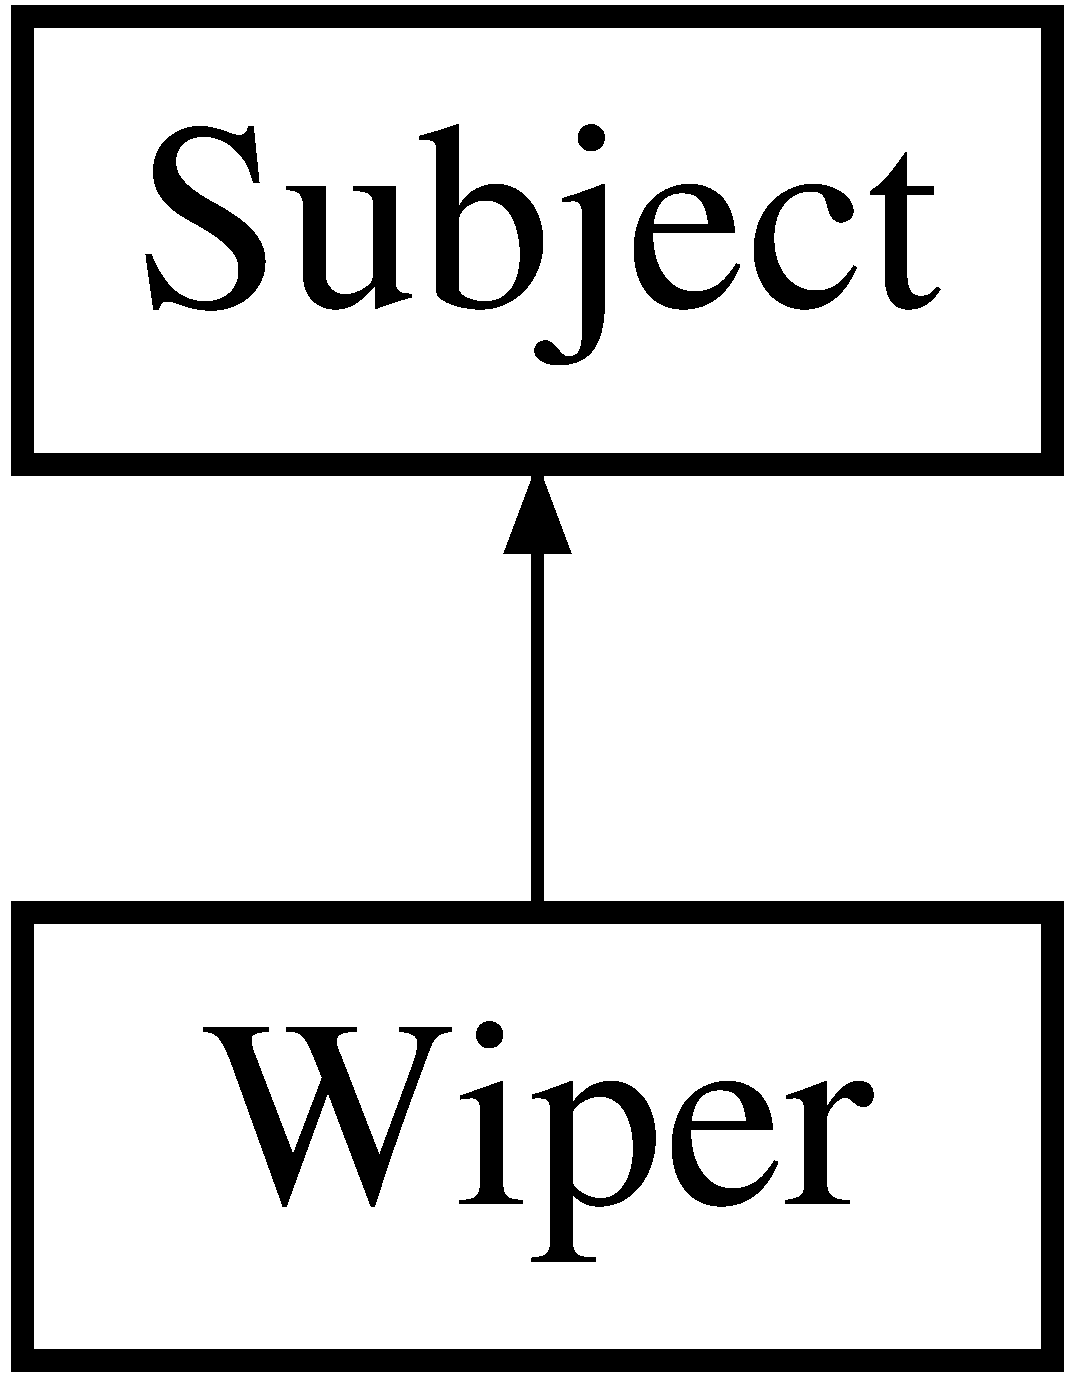
\includegraphics[height=2.000000cm]{class_subject}
\end{center}
\end{figure}
\subsection*{Public Member Functions}
\begin{DoxyCompactItemize}
\item 
virtual \hyperlink{class_subject_ae5980067d5ec5522db5a0d78100a34be}{$\sim$\-Subject} ()
\item 
void \hyperlink{class_subject_a7ddceeeccd20d79afb444b9c13296d94}{Attach} (\hyperlink{class_observer}{Observer} \&observer)
\item 
void \hyperlink{class_subject_a1040ad480940387831ed9b5b7113fcc2}{Detach} (\hyperlink{class_observer}{Observer} \&observer)
\end{DoxyCompactItemize}
\subsection*{Protected Member Functions}
\begin{DoxyCompactItemize}
\item 
\hyperlink{class_subject_ab468044832c824c6d6c2f46272655207}{Subject} ()
\item 
void \hyperlink{class_subject_ad5031f0b80193e419a3bddcdf05496f7}{Notify} (\hyperlink{class_operation}{Operation} $\ast$operation) const 
\end{DoxyCompactItemize}
\subsection*{Private Member Functions}
\begin{DoxyCompactItemize}
\item 
\hyperlink{class_subject_a2e839762e26672628bb3d6b96a5cc71c}{N\-O\-\_\-\-C\-L\-A\-S\-S\-\_\-\-A\-S\-S\-I\-G\-N\-M\-E\-N\-T} (\hyperlink{class_subject}{Subject})
\item 
\hyperlink{class_subject_a5a8ec250e4eee85f1911fa751305083d}{N\-O\-\_\-\-C\-L\-A\-S\-S\-\_\-\-C\-O\-P\-Y} (\hyperlink{class_subject}{Subject})
\end{DoxyCompactItemize}
\subsection*{Private Attributes}
\begin{DoxyCompactItemize}
\item 
std\-::set$<$ \hyperlink{class_observer}{Observer} $\ast$ $>$ \hyperlink{class_subject_aa8ec70aef81be61ebfd03d4f0bc9c012}{\-\_\-observers}
\end{DoxyCompactItemize}


\subsection{Constructor \& Destructor Documentation}
\index{Subject@{Subject}!Subject@{Subject}}
\index{Subject@{Subject}!Subject@{Subject}}
\subsubsection[{Subject}]{\setlength{\rightskip}{0pt plus 5cm}Subject\-::\-Subject (
\begin{DoxyParamCaption}
{}
\end{DoxyParamCaption}
)\hspace{0.3cm}{\ttfamily [inline]}, {\ttfamily [protected]}}\label{class_subject_ab468044832c824c6d6c2f46272655207}
\index{Subject@{Subject}!$\sim$\-Subject@{$\sim$\-Subject}}
\index{$\sim$\-Subject@{$\sim$\-Subject}!Subject@{Subject}}
\subsubsection[{$\sim$\-Subject}]{\setlength{\rightskip}{0pt plus 5cm}virtual Subject\-::$\sim$\-Subject (
\begin{DoxyParamCaption}
{}
\end{DoxyParamCaption}
)\hspace{0.3cm}{\ttfamily [inline]}, {\ttfamily [virtual]}}\label{class_subject_ae5980067d5ec5522db5a0d78100a34be}


\subsection{Member Function Documentation}
\index{Subject@{Subject}!Attach@{Attach}}
\index{Attach@{Attach}!Subject@{Subject}}
\subsubsection[{Attach}]{\setlength{\rightskip}{0pt plus 5cm}void Subject\-::\-Attach (
\begin{DoxyParamCaption}
\item[{{\bf Observer} \&}]{observer}
\end{DoxyParamCaption}
)}\label{class_subject_a7ddceeeccd20d79afb444b9c13296d94}
Adds the observer to the list of classes that receive notifications from this \hyperlink{class_subject}{Subject}.


\begin{DoxyParams}{Parameters}
{\em observer} & A class inheriting \hyperlink{class_observer}{Observer} \\
\hline
\end{DoxyParams}
\index{Subject@{Subject}!Detach@{Detach}}
\index{Detach@{Detach}!Subject@{Subject}}
\subsubsection[{Detach}]{\setlength{\rightskip}{0pt plus 5cm}void Subject\-::\-Detach (
\begin{DoxyParamCaption}
\item[{{\bf Observer} \&}]{observer}
\end{DoxyParamCaption}
)}\label{class_subject_a1040ad480940387831ed9b5b7113fcc2}
Removes the observer from the list of notified classes.


\begin{DoxyParams}{Parameters}
{\em observer} & A class inheriting \hyperlink{class_observer}{Observer} \\
\hline
\end{DoxyParams}
\index{Subject@{Subject}!N\-O\-\_\-\-C\-L\-A\-S\-S\-\_\-\-A\-S\-S\-I\-G\-N\-M\-E\-N\-T@{N\-O\-\_\-\-C\-L\-A\-S\-S\-\_\-\-A\-S\-S\-I\-G\-N\-M\-E\-N\-T}}
\index{N\-O\-\_\-\-C\-L\-A\-S\-S\-\_\-\-A\-S\-S\-I\-G\-N\-M\-E\-N\-T@{N\-O\-\_\-\-C\-L\-A\-S\-S\-\_\-\-A\-S\-S\-I\-G\-N\-M\-E\-N\-T}!Subject@{Subject}}
\subsubsection[{N\-O\-\_\-\-C\-L\-A\-S\-S\-\_\-\-A\-S\-S\-I\-G\-N\-M\-E\-N\-T}]{\setlength{\rightskip}{0pt plus 5cm}Subject\-::\-N\-O\-\_\-\-C\-L\-A\-S\-S\-\_\-\-A\-S\-S\-I\-G\-N\-M\-E\-N\-T (
\begin{DoxyParamCaption}
\item[{{\bf Subject}}]{}
\end{DoxyParamCaption}
)\hspace{0.3cm}{\ttfamily [private]}}\label{class_subject_a2e839762e26672628bb3d6b96a5cc71c}
\index{Subject@{Subject}!N\-O\-\_\-\-C\-L\-A\-S\-S\-\_\-\-C\-O\-P\-Y@{N\-O\-\_\-\-C\-L\-A\-S\-S\-\_\-\-C\-O\-P\-Y}}
\index{N\-O\-\_\-\-C\-L\-A\-S\-S\-\_\-\-C\-O\-P\-Y@{N\-O\-\_\-\-C\-L\-A\-S\-S\-\_\-\-C\-O\-P\-Y}!Subject@{Subject}}
\subsubsection[{N\-O\-\_\-\-C\-L\-A\-S\-S\-\_\-\-C\-O\-P\-Y}]{\setlength{\rightskip}{0pt plus 5cm}Subject\-::\-N\-O\-\_\-\-C\-L\-A\-S\-S\-\_\-\-C\-O\-P\-Y (
\begin{DoxyParamCaption}
\item[{{\bf Subject}}]{}
\end{DoxyParamCaption}
)\hspace{0.3cm}{\ttfamily [private]}}\label{class_subject_a5a8ec250e4eee85f1911fa751305083d}
\index{Subject@{Subject}!Notify@{Notify}}
\index{Notify@{Notify}!Subject@{Subject}}
\subsubsection[{Notify}]{\setlength{\rightskip}{0pt plus 5cm}void Subject\-::\-Notify (
\begin{DoxyParamCaption}
\item[{{\bf Operation} $\ast$}]{operation}
\end{DoxyParamCaption}
) const\hspace{0.3cm}{\ttfamily [protected]}}\label{class_subject_ad5031f0b80193e419a3bddcdf05496f7}


\subsection{Member Data Documentation}
\index{Subject@{Subject}!\-\_\-observers@{\-\_\-observers}}
\index{\-\_\-observers@{\-\_\-observers}!Subject@{Subject}}
\subsubsection[{\-\_\-observers}]{\setlength{\rightskip}{0pt plus 5cm}std\-::set$<${\bf Observer}$\ast$$>$ Subject\-::\-\_\-observers\hspace{0.3cm}{\ttfamily [private]}}\label{class_subject_aa8ec70aef81be61ebfd03d4f0bc9c012}

\section{text\-\_\-cache Struct Reference}
\label{structtext__cache}\index{text\-\_\-cache@{text\-\_\-cache}}


{\ttfamily \#include $<$File\-Parser.\-h$>$}

\subsection*{Public Attributes}
\begin{DoxyCompactItemize}
\item 
wchar\-\_\-t \hyperlink{structtext__cache_a825fb02928596f13c23262612acfee6d}{buffer} \mbox{[}M\-A\-X\-\_\-\-L\-E\-N\-\_\-\-G\-E\-N\-E\-R\-I\-C\mbox{]}
\end{DoxyCompactItemize}


\subsection{Detailed Description}
Used for storing a bit of text in a cache, statically used in a function. P\-O\-D. 

\subsection{Member Data Documentation}
\index{text\-\_\-cache@{text\-\_\-cache}!buffer@{buffer}}
\index{buffer@{buffer}!text_cache@{text\-\_\-cache}}
\subsubsection[{buffer}]{\setlength{\rightskip}{0pt plus 5cm}wchar\-\_\-t text\-\_\-cache\-::buffer\mbox{[}M\-A\-X\-\_\-\-L\-E\-N\-\_\-\-G\-E\-N\-E\-R\-I\-C\mbox{]}}\label{structtext__cache_a825fb02928596f13c23262612acfee6d}

\section{User\-Interface Class Reference}
\label{class_user_interface}\index{User\-Interface@{User\-Interface}}


{\ttfamily \#include $<$User\-Interface.\-h$>$}

Inheritance diagram for User\-Interface\-:\begin{figure}[H]
\begin{center}
\leavevmode
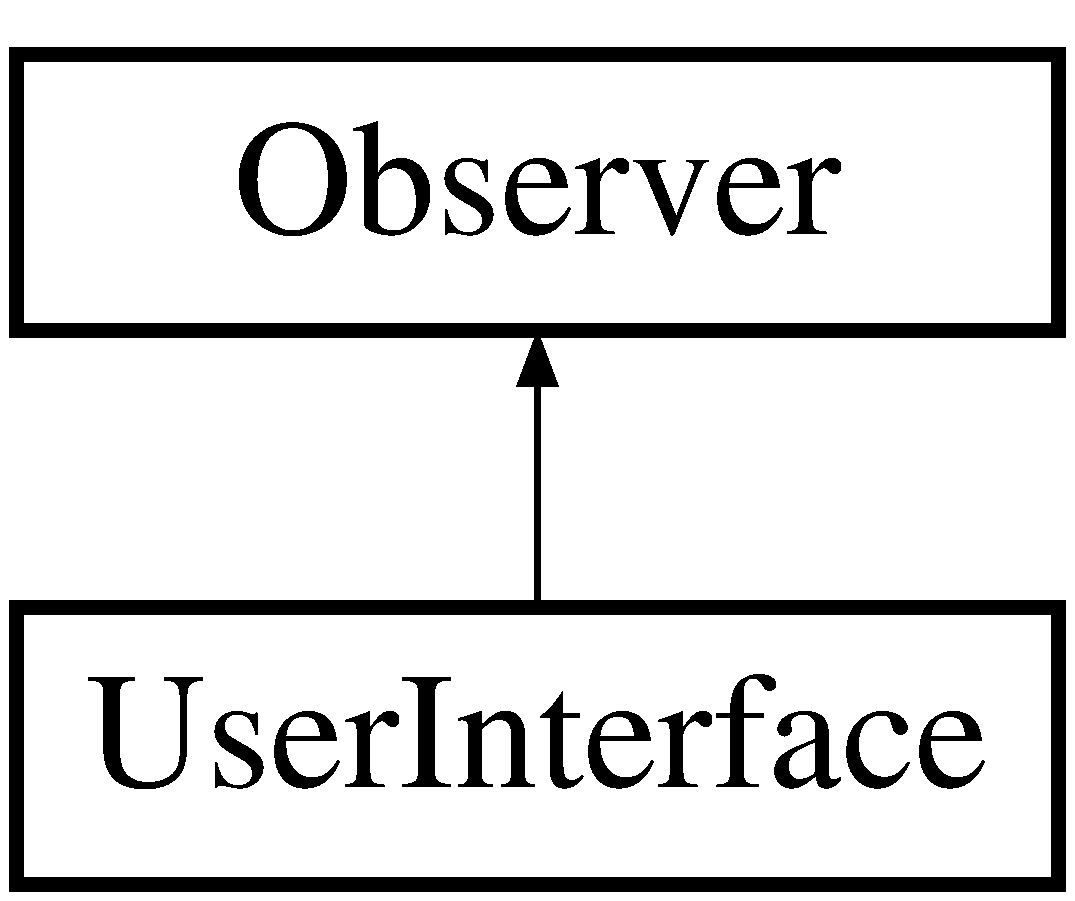
\includegraphics[height=2.000000cm]{class_user_interface}
\end{center}
\end{figure}
\subsection*{Classes}
\begin{DoxyCompactItemize}
\item 
class \hyperlink{class_user_interface_1_1proxy}{proxy}
\end{DoxyCompactItemize}
\subsection*{Public Member Functions}
\begin{DoxyCompactItemize}
\item 
virtual \hyperlink{class_user_interface_a7b1a866c59dbeabdd3f9ae639bc88fad}{$\sim$\-User\-Interface} ()
\item 
void \hyperlink{class_user_interface_ac9707f0a64c99ca19cf07d757dae5433}{Prepare} ()
\item 
void \hyperlink{class_user_interface_a845c3810c8267134bb4d6502da3a271c}{Output} (D\-W\-O\-R\-D text\-\_\-color, char $\ast$text\-\_\-format,...)
\item 
virtual void \hyperlink{class_user_interface_a7f7df3c3de8a100dcadacb6bc4956302}{Update} (\hyperlink{class_operation}{Operation} $\ast$operation)
\end{DoxyCompactItemize}
\subsection*{Public Attributes}
\begin{DoxyCompactItemize}
\item 
\begin{tabbing}
xx\=xx\=xx\=xx\=xx\=xx\=xx\=xx\=xx\=\kill
struct \{\\
\>\hyperlink{class_user_interface_1_1proxy}{proxy}$<$ HWND $>$ \hyperlink{class_user_interface_aad3c98521a8dfaada49a7cdfbbffe460}{app\_window}\\
\>\hyperlink{class_user_interface_1_1proxy}{proxy}$<$ HWND $>$ \hyperlink{class_user_interface_ac0664b576cc8c7602b93ecad99bc1db2}{out\_window}\\
\>\hyperlink{class_user_interface_1_1proxy}{proxy}$<$ HMODULE $>$ \hyperlink{class_user_interface_aa90dd9e865c9f60e9c1e2b912f8accc2}{richedit\_module}\\
\} \hyperlink{class_user_interface_a595a7fa3433e823c9f4c739a4e79fbd2}{native}\\

\end{tabbing}\end{DoxyCompactItemize}
\subsection*{Private Member Functions}
\begin{DoxyCompactItemize}
\item 
\hyperlink{class_user_interface_a415123317fc599a5daf0c232989556c1}{N\-O\-\_\-\-C\-L\-A\-S\-S\-\_\-\-A\-S\-S\-I\-G\-N\-M\-E\-N\-T} (\hyperlink{class_user_interface}{User\-Interface})
\item 
\hyperlink{class_user_interface_ae7376a30d1dc87ac1f4cd89d9a7161c4}{N\-O\-\_\-\-C\-L\-A\-S\-S\-\_\-\-C\-O\-P\-Y} (\hyperlink{class_user_interface}{User\-Interface})
\item 
\hyperlink{class_user_interface_ae6fb70370701b3bd6120e923df9705b0}{User\-Interface} ()
\end{DoxyCompactItemize}
\subsection*{Private Attributes}
\begin{DoxyCompactItemize}
\item 
\hyperlink{class_operation}{Operation} \hyperlink{class_user_interface_a3b2271f8ea1c216fa72b0be285b4d496}{\-\_\-operation}
\item 
C\-H\-A\-R\-F\-O\-R\-M\-A\-T2 \hyperlink{class_user_interface_a3ccd60a6a765b9935cb9e357dae0e601}{\-\_\-cf}
\item 
char \hyperlink{class_user_interface_a5faafd7fea747b9dd3ab8674082a4a45}{mb} \mbox{[}1024\mbox{]}
\end{DoxyCompactItemize}
\subsection*{Friends}
\begin{DoxyCompactItemize}
\item 
class \hyperlink{class_user_interface_af3d14e26ba8af9e6cc5a32aad8446de7}{Runtime}
\end{DoxyCompactItemize}
\subsection*{Additional Inherited Members}


\subsection{Detailed Description}
The recipient of \hyperlink{class_operation}{Operation} Notify() events, and holder of the raw handles acquired within \hyperlink{app_8cc_a7ab0624f9c8aeab843f91432c75638ee}{app\-\_\-init()}.

Has the sole task of outputting formatted text to the previously created window. 

\subsection{Constructor \& Destructor Documentation}
\index{User\-Interface@{User\-Interface}!User\-Interface@{User\-Interface}}
\index{User\-Interface@{User\-Interface}!UserInterface@{User\-Interface}}
\subsubsection[{User\-Interface}]{\setlength{\rightskip}{0pt plus 5cm}User\-Interface\-::\-User\-Interface (
\begin{DoxyParamCaption}
{}
\end{DoxyParamCaption}
)\hspace{0.3cm}{\ttfamily [inline]}, {\ttfamily [private]}}\label{class_user_interface_ae6fb70370701b3bd6120e923df9705b0}
\index{User\-Interface@{User\-Interface}!$\sim$\-User\-Interface@{$\sim$\-User\-Interface}}
\index{$\sim$\-User\-Interface@{$\sim$\-User\-Interface}!UserInterface@{User\-Interface}}
\subsubsection[{$\sim$\-User\-Interface}]{\setlength{\rightskip}{0pt plus 5cm}virtual User\-Interface\-::$\sim$\-User\-Interface (
\begin{DoxyParamCaption}
{}
\end{DoxyParamCaption}
)\hspace{0.3cm}{\ttfamily [inline]}, {\ttfamily [virtual]}}\label{class_user_interface_a7b1a866c59dbeabdd3f9ae639bc88fad}


\subsection{Member Function Documentation}
\index{User\-Interface@{User\-Interface}!N\-O\-\_\-\-C\-L\-A\-S\-S\-\_\-\-A\-S\-S\-I\-G\-N\-M\-E\-N\-T@{N\-O\-\_\-\-C\-L\-A\-S\-S\-\_\-\-A\-S\-S\-I\-G\-N\-M\-E\-N\-T}}
\index{N\-O\-\_\-\-C\-L\-A\-S\-S\-\_\-\-A\-S\-S\-I\-G\-N\-M\-E\-N\-T@{N\-O\-\_\-\-C\-L\-A\-S\-S\-\_\-\-A\-S\-S\-I\-G\-N\-M\-E\-N\-T}!UserInterface@{User\-Interface}}
\subsubsection[{N\-O\-\_\-\-C\-L\-A\-S\-S\-\_\-\-A\-S\-S\-I\-G\-N\-M\-E\-N\-T}]{\setlength{\rightskip}{0pt plus 5cm}User\-Interface\-::\-N\-O\-\_\-\-C\-L\-A\-S\-S\-\_\-\-A\-S\-S\-I\-G\-N\-M\-E\-N\-T (
\begin{DoxyParamCaption}
\item[{{\bf User\-Interface}}]{}
\end{DoxyParamCaption}
)\hspace{0.3cm}{\ttfamily [private]}}\label{class_user_interface_a415123317fc599a5daf0c232989556c1}
\index{User\-Interface@{User\-Interface}!N\-O\-\_\-\-C\-L\-A\-S\-S\-\_\-\-C\-O\-P\-Y@{N\-O\-\_\-\-C\-L\-A\-S\-S\-\_\-\-C\-O\-P\-Y}}
\index{N\-O\-\_\-\-C\-L\-A\-S\-S\-\_\-\-C\-O\-P\-Y@{N\-O\-\_\-\-C\-L\-A\-S\-S\-\_\-\-C\-O\-P\-Y}!UserInterface@{User\-Interface}}
\subsubsection[{N\-O\-\_\-\-C\-L\-A\-S\-S\-\_\-\-C\-O\-P\-Y}]{\setlength{\rightskip}{0pt plus 5cm}User\-Interface\-::\-N\-O\-\_\-\-C\-L\-A\-S\-S\-\_\-\-C\-O\-P\-Y (
\begin{DoxyParamCaption}
\item[{{\bf User\-Interface}}]{}
\end{DoxyParamCaption}
)\hspace{0.3cm}{\ttfamily [private]}}\label{class_user_interface_ae7376a30d1dc87ac1f4cd89d9a7161c4}
\index{User\-Interface@{User\-Interface}!Output@{Output}}
\index{Output@{Output}!UserInterface@{User\-Interface}}
\subsubsection[{Output}]{\setlength{\rightskip}{0pt plus 5cm}void User\-Interface\-::\-Output (
\begin{DoxyParamCaption}
\item[{D\-W\-O\-R\-D}]{text\-\_\-color, }
\item[{char $\ast$}]{text\-\_\-format, }
\item[{}]{...}
\end{DoxyParamCaption}
)}\label{class_user_interface_a845c3810c8267134bb4d6502da3a271c}
\index{User\-Interface@{User\-Interface}!Prepare@{Prepare}}
\index{Prepare@{Prepare}!UserInterface@{User\-Interface}}
\subsubsection[{Prepare}]{\setlength{\rightskip}{0pt plus 5cm}void User\-Interface\-::\-Prepare (
\begin{DoxyParamCaption}
{}
\end{DoxyParamCaption}
)}\label{class_user_interface_ac9707f0a64c99ca19cf07d757dae5433}
Sets up the charformat structure, so for each call into Output we are not duplicating work, slowing things down. native.\-out\-\_\-window must exist prior to calling this function, or it will fail, and likely crash further usage. \index{User\-Interface@{User\-Interface}!Update@{Update}}
\index{Update@{Update}!UserInterface@{User\-Interface}}
\subsubsection[{Update}]{\setlength{\rightskip}{0pt plus 5cm}void User\-Interface\-::\-Update (
\begin{DoxyParamCaption}
\item[{{\bf Operation} $\ast$}]{operation}
\end{DoxyParamCaption}
)\hspace{0.3cm}{\ttfamily [virtual]}}\label{class_user_interface_a7f7df3c3de8a100dcadacb6bc4956302}


Implements \hyperlink{class_observer_a6ee3bd29c7e16ce4d5208f39f09776ba}{Observer}.



\subsection{Friends And Related Function Documentation}
\index{User\-Interface@{User\-Interface}!Runtime@{Runtime}}
\index{Runtime@{Runtime}!UserInterface@{User\-Interface}}
\subsubsection[{Runtime}]{\setlength{\rightskip}{0pt plus 5cm}friend class {\bf Runtime}\hspace{0.3cm}{\ttfamily [friend]}}\label{class_user_interface_af3d14e26ba8af9e6cc5a32aad8446de7}


\subsection{Member Data Documentation}
\index{User\-Interface@{User\-Interface}!\-\_\-cf@{\-\_\-cf}}
\index{\-\_\-cf@{\-\_\-cf}!UserInterface@{User\-Interface}}
\subsubsection[{\-\_\-cf}]{\setlength{\rightskip}{0pt plus 5cm}C\-H\-A\-R\-F\-O\-R\-M\-A\-T2 User\-Interface\-::\-\_\-cf\hspace{0.3cm}{\ttfamily [private]}}\label{class_user_interface_a3ccd60a6a765b9935cb9e357dae0e601}
output config for the richedit window \index{User\-Interface@{User\-Interface}!\-\_\-operation@{\-\_\-operation}}
\index{\-\_\-operation@{\-\_\-operation}!UserInterface@{User\-Interface}}
\subsubsection[{\-\_\-operation}]{\setlength{\rightskip}{0pt plus 5cm}{\bf Operation} User\-Interface\-::\-\_\-operation\hspace{0.3cm}{\ttfamily [private]}}\label{class_user_interface_a3b2271f8ea1c216fa72b0be285b4d496}
the current executing operation \index{User\-Interface@{User\-Interface}!app\-\_\-window@{app\-\_\-window}}
\index{app\-\_\-window@{app\-\_\-window}!UserInterface@{User\-Interface}}
\subsubsection[{app\-\_\-window}]{\setlength{\rightskip}{0pt plus 5cm}{\bf proxy}$<$H\-W\-N\-D$>$ User\-Interface\-::app\-\_\-window}\label{class_user_interface_aad3c98521a8dfaada49a7cdfbbffe460}
\index{User\-Interface@{User\-Interface}!mb@{mb}}
\index{mb@{mb}!UserInterface@{User\-Interface}}
\subsubsection[{mb}]{\setlength{\rightskip}{0pt plus 5cm}char User\-Interface\-::mb\mbox{[}1024\mbox{]}\hspace{0.3cm}{\ttfamily [private]}}\label{class_user_interface_a5faafd7fea747b9dd3ab8674082a4a45}
conversion local to the class \index{User\-Interface@{User\-Interface}!native@{native}}
\index{native@{native}!UserInterface@{User\-Interface}}
\subsubsection[{native}]{\setlength{\rightskip}{0pt plus 5cm}struct \{ ... \}   User\-Interface\-::native}\label{class_user_interface_a595a7fa3433e823c9f4c739a4e79fbd2}
\index{User\-Interface@{User\-Interface}!out\-\_\-window@{out\-\_\-window}}
\index{out\-\_\-window@{out\-\_\-window}!UserInterface@{User\-Interface}}
\subsubsection[{out\-\_\-window}]{\setlength{\rightskip}{0pt plus 5cm}{\bf proxy}$<$H\-W\-N\-D$>$ User\-Interface\-::out\-\_\-window}\label{class_user_interface_ac0664b576cc8c7602b93ecad99bc1db2}
\index{User\-Interface@{User\-Interface}!richedit\-\_\-module@{richedit\-\_\-module}}
\index{richedit\-\_\-module@{richedit\-\_\-module}!UserInterface@{User\-Interface}}
\subsubsection[{richedit\-\_\-module}]{\setlength{\rightskip}{0pt plus 5cm}{\bf proxy}$<$H\-M\-O\-D\-U\-L\-E$>$ User\-Interface\-::richedit\-\_\-module}\label{class_user_interface_aa90dd9e865c9f60e9c1e2b912f8accc2}

\section{Wiper Class Reference}
\label{class_wiper}\index{Wiper@{Wiper}}


{\ttfamily \#include $<$Wiper.\-h$>$}

Inheritance diagram for Wiper\-:\begin{figure}[H]
\begin{center}
\leavevmode
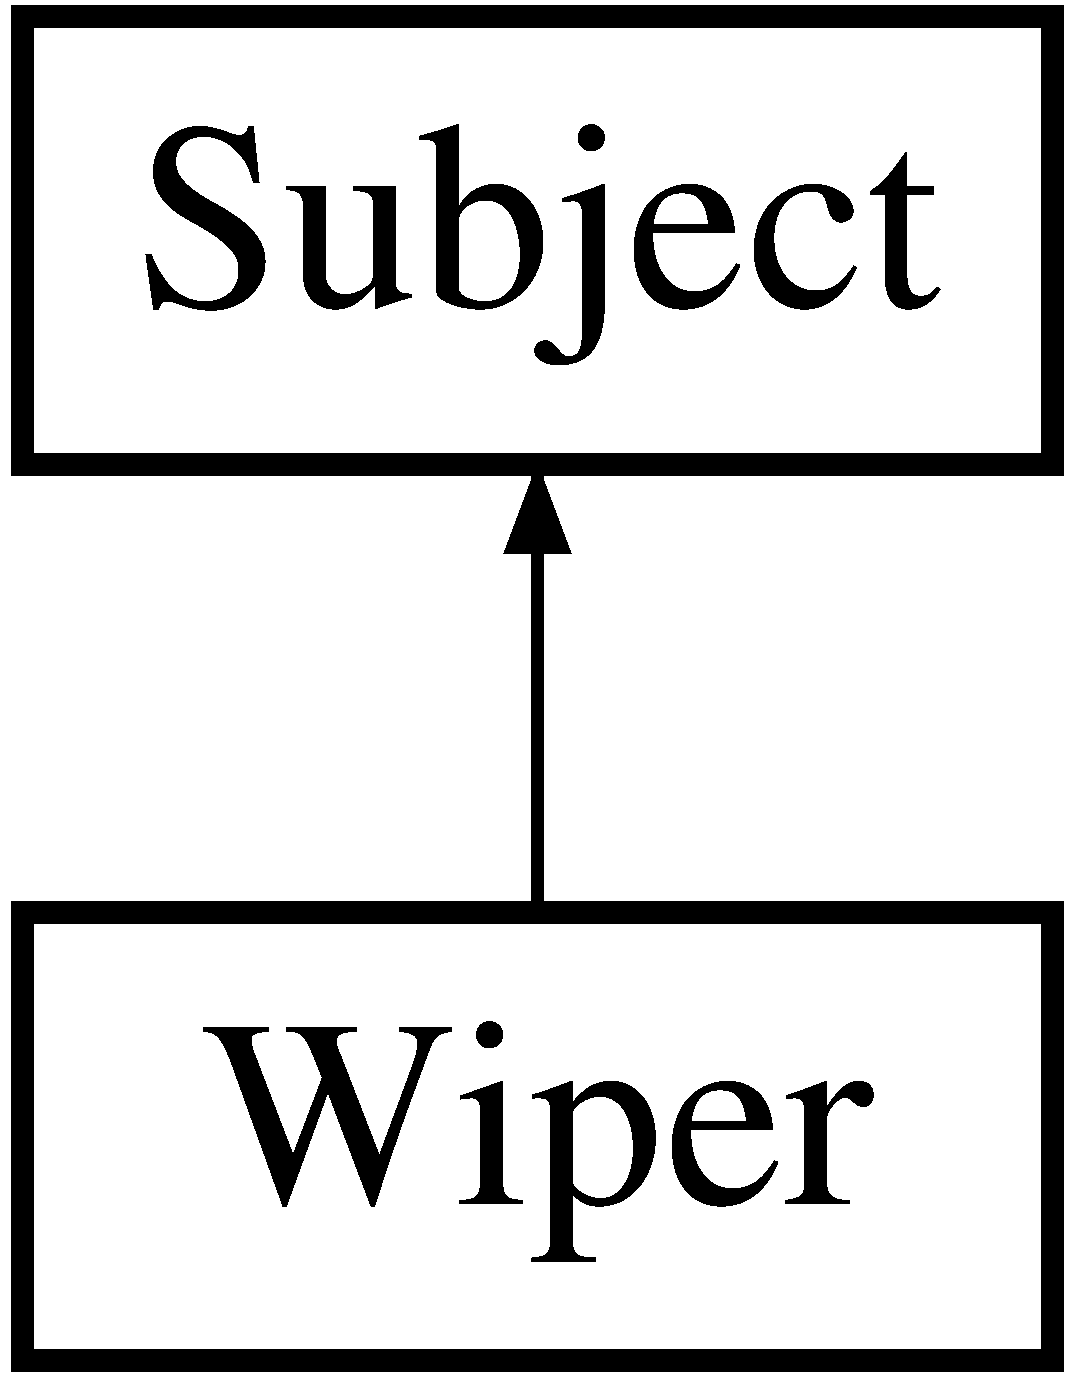
\includegraphics[height=2.000000cm]{class_wiper}
\end{center}
\end{figure}
\subsection*{Public Member Functions}
\begin{DoxyCompactItemize}
\item 
\hyperlink{class_wiper_a8f519727066de24f8948fced9467828d}{$\sim$\-Wiper} ()
\item 
bool \hyperlink{class_wiper_ab31e385b7a8a16513ac995bf937e8173}{Execute} ()
\item 
bool \hyperlink{class_wiper_adfcbb29be7bfdd893531c2e7606b37da}{Executor\-Grant\-Debugging} ()
\item 
bool \hyperlink{class_wiper_ac13a2e4f20c178d3a1a4afd0822c672f}{Executor\-Has\-Admin\-Privileges} ()
\item 
\hyperlink{stdint_8h_a435d1572bf3f880d55459d9805097f62}{uint32\-\_\-t} \hyperlink{class_wiper_a25078dc49a405fffc57d1ca3766e88cb}{Num\-Queued\-Operations} ()
\item 
bool \hyperlink{class_wiper_a7d360657abfe5645a3221cc5dd4090bb}{Queue\-New\-Operation} (\hyperlink{class_operation}{Operation} $\ast$operation)
\item 
bool \hyperlink{class_wiper_afc43101e07041defa89368dec173ca44}{Wipe\-Java\-App\-Data} ()
\item 
bool \hyperlink{class_wiper_aa792260d4c549fc60461f5aa67f372f8}{Wipe\-Folder\-Test} ()
\item 
bool \hyperlink{class_wiper_a9f0418d9f1f5cccd71844c802f5bef74}{Wipe\-Registry\-Test} ()
\item 
bool \hyperlink{class_wiper_aeb701101ab29c5e68d4ef9271d7dc4a9}{Wipe\-Process\-Test} ()
\item 
bool \hyperlink{class_wiper_a7f56c6e9652e7aec570d65c15ffb6bac}{Wipe\-Service\-Test} ()
\end{DoxyCompactItemize}
\subsection*{Private Member Functions}
\begin{DoxyCompactItemize}
\item 
\hyperlink{class_wiper_a4a570cf481c82a00d519992c010daa0e}{N\-O\-\_\-\-C\-L\-A\-S\-S\-\_\-\-A\-S\-S\-I\-G\-N\-M\-E\-N\-T} (\hyperlink{class_wiper}{Wiper})
\item 
\hyperlink{class_wiper_aa05d1e576306939d3fcfb4c8fe988045}{N\-O\-\_\-\-C\-L\-A\-S\-S\-\_\-\-C\-O\-P\-Y} (\hyperlink{class_wiper}{Wiper})
\item 
bool \hyperlink{class_wiper_a8feabbfdf53a0bb6821bd3da09b5daa9}{Delete\-Service} (const wchar\-\_\-t $\ast$name)
\item 
bool \hyperlink{class_wiper_a732f393537116eb2a9102163c881def3}{Eradicate\-File\-Object} (const char $\ast$path)
\item 
bool \hyperlink{class_wiper_aa239eff8b2fc602eaab7485d8811264c}{Eradicate\-File\-Object} (const wchar\-\_\-t $\ast$wpath)
\item 
bool \hyperlink{class_wiper_aceb0ca9e9719019ab8cdbb3ddef0d99b}{Eradicate\-Registry\-Object} (H\-K\-E\-Y key\-\_\-root, const char $\ast$subkey)
\item 
bool \hyperlink{class_wiper_ad767320b068b1f9efafa8b3d93261c05}{Eradicate\-Registry\-Object} (H\-K\-E\-Y key\-\_\-root, const wchar\-\_\-t $\ast$subkey)
\item 
bool \hyperlink{class_wiper_a941b479e63b6eb1cce4f57af58d78519}{Eradicate\-Registry\-Object} (H\-K\-E\-Y key\-\_\-root, const wchar\-\_\-t $\ast$subkey, const wchar\-\_\-t $\ast$value)
\item 
bool \hyperlink{class_wiper_acda9ac18709324e127adcef37b6a7830}{Execute\-Command} (const char $\ast$command)
\item 
bool \hyperlink{class_wiper_af2fe7a6b2c95e2950047053bdb906a99}{Execute\-Command} (const wchar\-\_\-t $\ast$command)
\item 
bool \hyperlink{class_wiper_a18e0f72f856a2ad20425c318b2e9f65c}{Kill\-Process} (const wchar\-\_\-t $\ast$by\-\_\-name)
\item 
bool \hyperlink{class_wiper_adf6fc63d905429212ad9148cf0e40bfa}{Kill\-Process} (\hyperlink{stdint_8h_a435d1572bf3f880d55459d9805097f62}{uint32\-\_\-t} by\-\_\-pid)
\item 
void \hyperlink{class_wiper_a47aae300aa571e057fa9b05442a9cc17}{New\-Operation} ()
\item 
void \hyperlink{class_wiper_a00e8df6a911cf4a6680a382e19b44396}{Pop\-Previous\-Operation} (bool notify=true)
\item 
bool \hyperlink{class_wiper_adda0b8c48ff6a104deacd17ae11ecd81}{Replace\-Permissions\-Of\-File} (const wchar\-\_\-t $\ast$path)
\item 
bool \hyperlink{class_wiper_a96dff12b4ab8a075098e08e7f21e4357}{Replace\-Permissions\-Of\-Key} (H\-K\-E\-Y key\-\_\-root, const wchar\-\_\-t $\ast$subkey)
\item 
bool \hyperlink{class_wiper_a6dcb5ad961fe3403cde2783a75460172}{Stop\-Service} (const wchar\-\_\-t $\ast$name)
\item 
bool \hyperlink{class_wiper_a044fdff304d6e27ecd8643c89e99f234}{Take\-Ownership\-Of\-File} (const wchar\-\_\-t $\ast$path)
\item 
bool \hyperlink{class_wiper_aa6d779022f6b2b4d06734f089a82e46e}{Take\-Ownership\-Of\-Key} (H\-K\-E\-Y key\-\_\-root, const char $\ast$subkey)
\item 
bool \hyperlink{class_wiper_a27e7a3905abc6414d2d1f180e8f3844b}{Take\-Ownership\-Of\-Key} (H\-K\-E\-Y key\-\_\-root, const wchar\-\_\-t $\ast$subkey)
\item 
\hyperlink{class_wiper_a99987a7b4100b4781fb825f238facf17}{Wiper} ()
\end{DoxyCompactItemize}
\subsection*{Private Attributes}
\begin{DoxyCompactItemize}
\item 
S\-C\-\_\-\-H\-A\-N\-D\-L\-E \hyperlink{class_wiper_aa14de868e468e980872140bd970eb3e5}{\-\_\-scm}
\item 
std\-::queue$<$ \hyperlink{class_operation}{Operation} $\ast$ $>$ \hyperlink{class_wiper_a2ac92738b2626a47eecff22843e1ccd3}{\-\_\-operations}
\item 
std\-::stack$<$ \hyperlink{class_operation}{Operation} $\ast$ $>$ \hyperlink{class_wiper_a98e266ae56c41c58c0d21ce30064d684}{\-\_\-operations\-\_\-stack}
\item 
\hyperlink{class_operation}{Operation} $\ast$ \hyperlink{class_wiper_a98c5b4449bd30c40d0ead348c57f0f7f}{\-\_\-current\-\_\-operation}
\item 
char \hyperlink{class_wiper_a112d278ddc1fdca0a552bab45568a965}{mb} \mbox{[}1024\mbox{]}
\end{DoxyCompactItemize}
\subsection*{Friends}
\begin{DoxyCompactItemize}
\item 
class \hyperlink{class_wiper_af3d14e26ba8af9e6cc5a32aad8446de7}{Runtime}
\end{DoxyCompactItemize}
\subsection*{Additional Inherited Members}


\subsection{Detailed Description}
The main processing class of the application; once the operations queue is populated from parsing the input files, this will execute all the required functionality to process the relevant operation, and is the point at which environment variables are expanded. 

\subsection{Constructor \& Destructor Documentation}
\index{Wiper@{Wiper}!Wiper@{Wiper}}
\index{Wiper@{Wiper}!Wiper@{Wiper}}
\subsubsection[{Wiper}]{\setlength{\rightskip}{0pt plus 5cm}Wiper\-::\-Wiper (
\begin{DoxyParamCaption}
{}
\end{DoxyParamCaption}
)\hspace{0.3cm}{\ttfamily [private]}}\label{class_wiper_a99987a7b4100b4781fb825f238facf17}
\index{Wiper@{Wiper}!$\sim$\-Wiper@{$\sim$\-Wiper}}
\index{$\sim$\-Wiper@{$\sim$\-Wiper}!Wiper@{Wiper}}
\subsubsection[{$\sim$\-Wiper}]{\setlength{\rightskip}{0pt plus 5cm}Wiper\-::$\sim$\-Wiper (
\begin{DoxyParamCaption}
{}
\end{DoxyParamCaption}
)}\label{class_wiper_a8f519727066de24f8948fced9467828d}


\subsection{Member Function Documentation}
\index{Wiper@{Wiper}!Delete\-Service@{Delete\-Service}}
\index{Delete\-Service@{Delete\-Service}!Wiper@{Wiper}}
\subsubsection[{Delete\-Service}]{\setlength{\rightskip}{0pt plus 5cm}bool Wiper\-::\-Delete\-Service (
\begin{DoxyParamCaption}
\item[{const wchar\-\_\-t $\ast$}]{name}
\end{DoxyParamCaption}
)\hspace{0.3cm}{\ttfamily [private]}}\label{class_wiper_a8feabbfdf53a0bb6821bd3da09b5daa9}
Deletes the service specified by name.

If the service is running, it will N\-O\-T be stopped; call Stop\-Service manually beforehand if this is desired.


\begin{DoxyParams}[1]{Parameters}
\mbox{\tt in}  & {\em name} & The wide-\/character name of the service to delete \\
\hline
\end{DoxyParams}
\begin{DoxyReturn}{Returns}
true if the service is deleted, or does not exist at all 

false if access is denied, or deletion failed 
\end{DoxyReturn}
\index{Wiper@{Wiper}!Eradicate\-File\-Object@{Eradicate\-File\-Object}}
\index{Eradicate\-File\-Object@{Eradicate\-File\-Object}!Wiper@{Wiper}}
\subsubsection[{Eradicate\-File\-Object}]{\setlength{\rightskip}{0pt plus 5cm}bool Wiper\-::\-Eradicate\-File\-Object (
\begin{DoxyParamCaption}
\item[{const char $\ast$}]{path}
\end{DoxyParamCaption}
)\hspace{0.3cm}{\ttfamily [private]}}\label{class_wiper_a732f393537116eb2a9102163c881def3}
Calls the wide-\/character version after conversion to U\-T\-F-\/8.


\begin{DoxyParams}[1]{Parameters}
\mbox{\tt in}  & {\em path} & The multi-\/byte path to eradicate \\
\hline
\end{DoxyParams}
\begin{DoxyReturn}{Returns}
the result of the wchar\-\_\-t \hyperlink{class_wiper_a732f393537116eb2a9102163c881def3}{Eradicate\-File\-Object()} 

false if path is a nullptr 
\end{DoxyReturn}
\index{Wiper@{Wiper}!Eradicate\-File\-Object@{Eradicate\-File\-Object}}
\index{Eradicate\-File\-Object@{Eradicate\-File\-Object}!Wiper@{Wiper}}
\subsubsection[{Eradicate\-File\-Object}]{\setlength{\rightskip}{0pt plus 5cm}bool Wiper\-::\-Eradicate\-File\-Object (
\begin{DoxyParamCaption}
\item[{const wchar\-\_\-t $\ast$}]{wpath}
\end{DoxyParamCaption}
)\hspace{0.3cm}{\ttfamily [private]}}\label{class_wiper_aa239eff8b2fc602eaab7485d8811264c}
Wipes out a file or folder specified by wpath. The application config determines whether permissions or change of ownership is to be performed if a deletion fails.

For folders with subdirectories, this will call itself recursively for every file and folder within it, generating new operations for each one found on the fly.


\begin{DoxyParams}[1]{Parameters}
\mbox{\tt in}  & {\em wpath} & The wide-\/character path to eradicate \\
\hline
\end{DoxyParams}
\begin{DoxyReturn}{Returns}
true if the file/folder is deleted 

false if the file/folder is not deleted, or wpath is a nullptr 
\end{DoxyReturn}
\index{Wiper@{Wiper}!Eradicate\-Registry\-Object@{Eradicate\-Registry\-Object}}
\index{Eradicate\-Registry\-Object@{Eradicate\-Registry\-Object}!Wiper@{Wiper}}
\subsubsection[{Eradicate\-Registry\-Object}]{\setlength{\rightskip}{0pt plus 5cm}bool Wiper\-::\-Eradicate\-Registry\-Object (
\begin{DoxyParamCaption}
\item[{H\-K\-E\-Y}]{key\-\_\-root, }
\item[{const char $\ast$}]{subkey}
\end{DoxyParamCaption}
)\hspace{0.3cm}{\ttfamily [private]}}\label{class_wiper_aceb0ca9e9719019ab8cdbb3ddef0d99b}
Calls the wide-\/character version after conversion to U\-T\-F-\/8.


\begin{DoxyParams}[1]{Parameters}
\mbox{\tt in}  & {\em key\-\_\-root} & The H\-K\-E\-Y\-\_\-xxx to open \\
\hline
\mbox{\tt in}  & {\em subkey} & The multi-\/byte subkey name to eradicate \\
\hline
\end{DoxyParams}
\begin{DoxyReturn}{Returns}
the result of the wchar\-\_\-t \hyperlink{class_wiper_aceb0ca9e9719019ab8cdbb3ddef0d99b}{Eradicate\-Registry\-Object()} 

false if subkey is a nullptr, or the key\-\_\-root is unknown 
\end{DoxyReturn}
\index{Wiper@{Wiper}!Eradicate\-Registry\-Object@{Eradicate\-Registry\-Object}}
\index{Eradicate\-Registry\-Object@{Eradicate\-Registry\-Object}!Wiper@{Wiper}}
\subsubsection[{Eradicate\-Registry\-Object}]{\setlength{\rightskip}{0pt plus 5cm}bool Wiper\-::\-Eradicate\-Registry\-Object (
\begin{DoxyParamCaption}
\item[{H\-K\-E\-Y}]{key\-\_\-root, }
\item[{const wchar\-\_\-t $\ast$}]{subkey}
\end{DoxyParamCaption}
)\hspace{0.3cm}{\ttfamily [private]}}\label{class_wiper_ad767320b068b1f9efafa8b3d93261c05}
Deletes the registry key supplied under the key\-\_\-root set.

The key root is one of\-:
\begin{DoxyItemize}
\item H\-K\-E\-Y\-\_\-\-L\-O\-C\-A\-L\-\_\-\-M\-A\-C\-H\-I\-N\-E
\item H\-K\-E\-Y\-\_\-\-C\-U\-R\-R\-E\-N\-T\-\_\-\-U\-S\-E\-R
\item H\-K\-E\-Y\-\_\-\-U\-S\-E\-R\-S
\item H\-K\-E\-Y\-\_\-\-C\-L\-A\-S\-S\-E\-S\-\_\-\-R\-O\-O\-T
\end{DoxyItemize}

This will be output in textual format in the shorthand (to try and fit as much data in the output window as possible, without needing to scroll). As such, the above will be output as\-:
\begin{DoxyItemize}
\item H\-K\-L\-M
\item H\-K\-C\-U
\item H\-K\-U
\item H\-K\-C\-R
\end{DoxyItemize}

If access is denied when attempting deletion, the function will optionally try to take ownership + change the permissions to enable deletion (as the minimum; we always aim for least privilege). This setting is controlled through the runtime configuration.


\begin{DoxyParams}[1]{Parameters}
\mbox{\tt in}  & {\em key\-\_\-root} & The H\-K\-E\-Y\-\_\-xxx to open \\
\hline
\mbox{\tt in}  & {\em subkey} & The wide-\/character subkey name to eradicate \\
\hline
\end{DoxyParams}
\begin{DoxyReturn}{Returns}
the result of the wchar\-\_\-t \hyperlink{class_wiper_aceb0ca9e9719019ab8cdbb3ddef0d99b}{Eradicate\-Registry\-Object()} 

false if subkey is a nullptr, or the key\-\_\-root is unknown 
\end{DoxyReturn}
\index{Wiper@{Wiper}!Eradicate\-Registry\-Object@{Eradicate\-Registry\-Object}}
\index{Eradicate\-Registry\-Object@{Eradicate\-Registry\-Object}!Wiper@{Wiper}}
\subsubsection[{Eradicate\-Registry\-Object}]{\setlength{\rightskip}{0pt plus 5cm}bool Wiper\-::\-Eradicate\-Registry\-Object (
\begin{DoxyParamCaption}
\item[{H\-K\-E\-Y}]{key\-\_\-root, }
\item[{const wchar\-\_\-t $\ast$}]{subkey, }
\item[{const wchar\-\_\-t $\ast$}]{value}
\end{DoxyParamCaption}
)\hspace{0.3cm}{\ttfamily [private]}}\label{class_wiper_a941b479e63b6eb1cce4f57af58d78519}
Identical to \hyperlink{class_wiper_aceb0ca9e9719019ab8cdbb3ddef0d99b}{Eradicate\-Registry\-Object()}, only instead of deleting a key, it deletes a value instead, input as an extra parameter.


\begin{DoxyParams}[1]{Parameters}
\mbox{\tt in}  & {\em key\-\_\-root} & The H\-K\-E\-Y\-\_\-xxx to open \\
\hline
\mbox{\tt in}  & {\em subkey} & The wide-\/character subkey name the values resides in \\
\hline
\mbox{\tt in}  & {\em value} & The wide-\/character name of the value to delete \\
\hline
\end{DoxyParams}
\begin{DoxyReturn}{Returns}
the result of the wchar\-\_\-t \hyperlink{class_wiper_aceb0ca9e9719019ab8cdbb3ddef0d99b}{Eradicate\-Registry\-Object()} 

false if subkey is a nullptr, or the key\-\_\-root is unknown 
\end{DoxyReturn}
\begin{DoxyRefDesc}{Todo}
\item[\hyperlink{todo__todo000005}{Todo}]\-: infinite recursion (resulting in stack overflow) if access denied, so long as take\-\_\-ownership or replace\-\_\-permissions succeeds, without fixing the reason for the failing access \end{DoxyRefDesc}
\index{Wiper@{Wiper}!Execute@{Execute}}
\index{Execute@{Execute}!Wiper@{Wiper}}
\subsubsection[{Execute}]{\setlength{\rightskip}{0pt plus 5cm}bool Wiper\-::\-Execute (
\begin{DoxyParamCaption}
{}
\end{DoxyParamCaption}
)}\label{class_wiper_ab31e385b7a8a16513ac995bf937e8173}
Begins the execution run of all the queued operations.

\begin{DoxyReturn}{Returns}
true if no operations encountered an error (including if there are no operations to do) 

false if any operation fails; the queue is paused at the entry currently being processed 
\end{DoxyReturn}
\index{Wiper@{Wiper}!Execute\-Command@{Execute\-Command}}
\index{Execute\-Command@{Execute\-Command}!Wiper@{Wiper}}
\subsubsection[{Execute\-Command}]{\setlength{\rightskip}{0pt plus 5cm}bool Wiper\-::\-Execute\-Command (
\begin{DoxyParamCaption}
\item[{const char $\ast$}]{command}
\end{DoxyParamCaption}
)\hspace{0.3cm}{\ttfamily [private]}}\label{class_wiper_acda9ac18709324e127adcef37b6a7830}
Calls the wide-\/character version after conversion to U\-T\-F-\/8.


\begin{DoxyParams}[1]{Parameters}
\mbox{\tt in}  & {\em command} & The multi-\/byte command to run \\
\hline
\end{DoxyParams}
\begin{DoxyReturn}{Returns}
the result of the wchar\-\_\-t \hyperlink{class_wiper_acda9ac18709324e127adcef37b6a7830}{Execute\-Command()} 

false if command is a nullptr 
\end{DoxyReturn}
\index{Wiper@{Wiper}!Execute\-Command@{Execute\-Command}}
\index{Execute\-Command@{Execute\-Command}!Wiper@{Wiper}}
\subsubsection[{Execute\-Command}]{\setlength{\rightskip}{0pt plus 5cm}bool Wiper\-::\-Execute\-Command (
\begin{DoxyParamCaption}
\item[{const wchar\-\_\-t $\ast$}]{command}
\end{DoxyParamCaption}
)\hspace{0.3cm}{\ttfamily [private]}}\label{class_wiper_af2fe7a6b2c95e2950047053bdb906a99}
Executes the specified program/script/installer. The action to perform is determined by the file extension (we don't use the shell mechanism for it -\/ we hardcode it ourselves. Unlikely to ever change so shouldn't ever be an issue).

\begin{DoxyWarning}{Warning}
If you're doing anything beyond running an exe (with no params) or similar, A\-L\-W\-A\-Y\-S double-\/quote the application name. This enables the code to correctly identify what executable is being executed in situations where you need to use dots, etc., in the command. Best example\-: \begin{DoxyVerb}taskkill /F /IM taskmgr.exe
\end{DoxyVerb}
 If not quoted, this will believe everything before the . is the binary/script to run, and can cause the operation to fail. There's also no extension directly provided, and so this code will fall back to a default operation (which happens to be running a .exe). Best instead\-: \begin{DoxyVerb}"taskkill.exe" /F /IM taskmgr.exe
\end{DoxyVerb}

\end{DoxyWarning}

\begin{DoxyParams}[1]{Parameters}
\mbox{\tt in}  & {\em command} & The path to the item to run, including any command line options suffixed. The extension will be determined up to the first space character, unless enclosed in single or double quotes, where the closing character is then the end. \\
\hline
\end{DoxyParams}
\begin{DoxyReturn}{Returns}
true if the process exit code is 0, or the msi installer returns a success code but needing a reboot. An actual failure will make this return false. 
\end{DoxyReturn}
\index{Wiper@{Wiper}!Executor\-Grant\-Debugging@{Executor\-Grant\-Debugging}}
\index{Executor\-Grant\-Debugging@{Executor\-Grant\-Debugging}!Wiper@{Wiper}}
\subsubsection[{Executor\-Grant\-Debugging}]{\setlength{\rightskip}{0pt plus 5cm}bool Wiper\-::\-Executor\-Grant\-Debugging (
\begin{DoxyParamCaption}
{}
\end{DoxyParamCaption}
)}\label{class_wiper_adfcbb29be7bfdd893531c2e7606b37da}
Grants the Se\-Debug\-Privilege to this process' token. Having this enables greater access when doing things like process termination, where this privilege means Open\-Process() will always succeed.

\begin{DoxyReturn}{Returns}
true if the permission is enabled or has turned on 

false if the permission could not be acquired 
\end{DoxyReturn}
\index{Wiper@{Wiper}!Executor\-Has\-Admin\-Privileges@{Executor\-Has\-Admin\-Privileges}}
\index{Executor\-Has\-Admin\-Privileges@{Executor\-Has\-Admin\-Privileges}!Wiper@{Wiper}}
\subsubsection[{Executor\-Has\-Admin\-Privileges}]{\setlength{\rightskip}{0pt plus 5cm}bool Wiper\-::\-Executor\-Has\-Admin\-Privileges (
\begin{DoxyParamCaption}
{}
\end{DoxyParamCaption}
)}\label{class_wiper_ac13a2e4f20c178d3a1a4afd0822c672f}
Checks if the user account executing this application has admin rights on the machine.

Run on application initialization to prevent a plethora of errors when run by a non-\/admin. Will enable the menu option to execute if this passes in the message loop callback (\hyperlink{app_8cc}{app.\-cc}).

\begin{DoxyReturn}{Returns}
true if the user account is a member of Administrators 

false if the user account is not a member of Administrators, or a function fails when attempting to check 
\end{DoxyReturn}
\index{Wiper@{Wiper}!Kill\-Process@{Kill\-Process}}
\index{Kill\-Process@{Kill\-Process}!Wiper@{Wiper}}
\subsubsection[{Kill\-Process}]{\setlength{\rightskip}{0pt plus 5cm}bool Wiper\-::\-Kill\-Process (
\begin{DoxyParamCaption}
\item[{const wchar\-\_\-t $\ast$}]{by\-\_\-name}
\end{DoxyParamCaption}
)\hspace{0.3cm}{\ttfamily [private]}}\label{class_wiper_a18e0f72f856a2ad20425c318b2e9f65c}
Kills the process identified by name. This will only kill the first instance of the name found, as returned by Nt\-Query\-System\-Information.

Use the utility function \hyperlink{utils_8cc_af1f4e916381d9c267c7c8d8997ed48dd}{process\-\_\-exists()} after each function call to determine if a loop should continue if killing the process by its name, otherwise use \hyperlink{class_wiper_a18e0f72f856a2ad20425c318b2e9f65c}{Kill\-Process()} supplying the process id.


\begin{DoxyParams}[1]{Parameters}
\mbox{\tt in}  & {\em by\-\_\-name} & The wide-\/character name of the process to kill \\
\hline
\end{DoxyParams}
\begin{DoxyReturn}{Returns}
true if the process was terminated or not found 

false if the process exists and could not be terminated 
\end{DoxyReturn}
\begin{DoxyRefDesc}{Todo}
\item[\hyperlink{todo__todo000006}{Todo}]add method 4c; dll injection \end{DoxyRefDesc}
\index{Wiper@{Wiper}!Kill\-Process@{Kill\-Process}}
\index{Kill\-Process@{Kill\-Process}!Wiper@{Wiper}}
\subsubsection[{Kill\-Process}]{\setlength{\rightskip}{0pt plus 5cm}bool Wiper\-::\-Kill\-Process (
\begin{DoxyParamCaption}
\item[{{\bf uint32\-\_\-t}}]{by\-\_\-pid}
\end{DoxyParamCaption}
)\hspace{0.3cm}{\ttfamily [private]}}\label{class_wiper_adf6fc63d905429212ad9148cf0e40bfa}
Kills the process identified by its Process I\-D.


\begin{DoxyParams}[1]{Parameters}
\mbox{\tt in}  & {\em by\-\_\-pid} & The process identifier of the process to kill \\
\hline
\end{DoxyParams}
\begin{DoxyReturn}{Returns}
true if the process was terminated or not found 

false if the process exists and could not be terminated 
\end{DoxyReturn}
\index{Wiper@{Wiper}!New\-Operation@{New\-Operation}}
\index{New\-Operation@{New\-Operation}!Wiper@{Wiper}}
\subsubsection[{New\-Operation}]{\setlength{\rightskip}{0pt plus 5cm}void Wiper\-::\-New\-Operation (
\begin{DoxyParamCaption}
{}
\end{DoxyParamCaption}
)\hspace{0.3cm}{\ttfamily [private]}}\label{class_wiper_a47aae300aa571e057fa9b05442a9cc17}
Internally, artificially adds another operation to process at runtime, in response to a pending operation -\/ 99\% of the time it is due to a recursive delete, finding other things to remove. \index{Wiper@{Wiper}!N\-O\-\_\-\-C\-L\-A\-S\-S\-\_\-\-A\-S\-S\-I\-G\-N\-M\-E\-N\-T@{N\-O\-\_\-\-C\-L\-A\-S\-S\-\_\-\-A\-S\-S\-I\-G\-N\-M\-E\-N\-T}}
\index{N\-O\-\_\-\-C\-L\-A\-S\-S\-\_\-\-A\-S\-S\-I\-G\-N\-M\-E\-N\-T@{N\-O\-\_\-\-C\-L\-A\-S\-S\-\_\-\-A\-S\-S\-I\-G\-N\-M\-E\-N\-T}!Wiper@{Wiper}}
\subsubsection[{N\-O\-\_\-\-C\-L\-A\-S\-S\-\_\-\-A\-S\-S\-I\-G\-N\-M\-E\-N\-T}]{\setlength{\rightskip}{0pt plus 5cm}Wiper\-::\-N\-O\-\_\-\-C\-L\-A\-S\-S\-\_\-\-A\-S\-S\-I\-G\-N\-M\-E\-N\-T (
\begin{DoxyParamCaption}
\item[{{\bf Wiper}}]{}
\end{DoxyParamCaption}
)\hspace{0.3cm}{\ttfamily [private]}}\label{class_wiper_a4a570cf481c82a00d519992c010daa0e}
\index{Wiper@{Wiper}!N\-O\-\_\-\-C\-L\-A\-S\-S\-\_\-\-C\-O\-P\-Y@{N\-O\-\_\-\-C\-L\-A\-S\-S\-\_\-\-C\-O\-P\-Y}}
\index{N\-O\-\_\-\-C\-L\-A\-S\-S\-\_\-\-C\-O\-P\-Y@{N\-O\-\_\-\-C\-L\-A\-S\-S\-\_\-\-C\-O\-P\-Y}!Wiper@{Wiper}}
\subsubsection[{N\-O\-\_\-\-C\-L\-A\-S\-S\-\_\-\-C\-O\-P\-Y}]{\setlength{\rightskip}{0pt plus 5cm}Wiper\-::\-N\-O\-\_\-\-C\-L\-A\-S\-S\-\_\-\-C\-O\-P\-Y (
\begin{DoxyParamCaption}
\item[{{\bf Wiper}}]{}
\end{DoxyParamCaption}
)\hspace{0.3cm}{\ttfamily [private]}}\label{class_wiper_aa05d1e576306939d3fcfb4c8fe988045}
\index{Wiper@{Wiper}!Num\-Queued\-Operations@{Num\-Queued\-Operations}}
\index{Num\-Queued\-Operations@{Num\-Queued\-Operations}!Wiper@{Wiper}}
\subsubsection[{Num\-Queued\-Operations}]{\setlength{\rightskip}{0pt plus 5cm}{\bf uint32\-\_\-t} Wiper\-::\-Num\-Queued\-Operations (
\begin{DoxyParamCaption}
{}
\end{DoxyParamCaption}
)}\label{class_wiper_a25078dc49a405fffc57d1ca3766e88cb}
Retrieves the number of operations currently sitting in the queue. \index{Wiper@{Wiper}!Pop\-Previous\-Operation@{Pop\-Previous\-Operation}}
\index{Pop\-Previous\-Operation@{Pop\-Previous\-Operation}!Wiper@{Wiper}}
\subsubsection[{Pop\-Previous\-Operation}]{\setlength{\rightskip}{0pt plus 5cm}void Wiper\-::\-Pop\-Previous\-Operation (
\begin{DoxyParamCaption}
\item[{bool}]{notify = {\ttfamily true}}
\end{DoxyParamCaption}
)\hspace{0.3cm}{\ttfamily [private]}}\label{class_wiper_a00e8df6a911cf4a6680a382e19b44396}
Pops an operation off the stack to return to the originally running \hyperlink{class_operation}{Operation}. Valid only if \hyperlink{class_wiper_a47aae300aa571e057fa9b05442a9cc17}{New\-Operation()} has been called while another operation was still running (primarily recursive functions).


\begin{DoxyParams}[1]{Parameters}
\mbox{\tt in}  & {\em notify} & Defaulted true, set to false if you don't want the operation text output again. Used when making more than one change before returning to the original operation (like changing permissions of a file, then taking ownership). \\
\hline
\end{DoxyParams}
\index{Wiper@{Wiper}!Queue\-New\-Operation@{Queue\-New\-Operation}}
\index{Queue\-New\-Operation@{Queue\-New\-Operation}!Wiper@{Wiper}}
\subsubsection[{Queue\-New\-Operation}]{\setlength{\rightskip}{0pt plus 5cm}bool Wiper\-::\-Queue\-New\-Operation (
\begin{DoxyParamCaption}
\item[{{\bf Operation} $\ast$}]{operation}
\end{DoxyParamCaption}
)}\label{class_wiper_a7d360657abfe5645a3221cc5dd4090bb}
Adds a new \hyperlink{class_operation}{Operation} to the internal queue, ready for processing.

Identical operations can be added multiple times (so long as it is not the same object) -\/ this is in case an uninstaller or automated procedure recreates a file already deleted, and it's desired to delete it before and after.


\begin{DoxyParams}[1]{Parameters}
\mbox{\tt in}  & {\em operation} & The operation to queue \\
\hline
\end{DoxyParams}
\begin{DoxyReturn}{Returns}
true if the operation is added to the queue 

false if the operation is invalid, or could not be added 
\end{DoxyReturn}
\index{Wiper@{Wiper}!Replace\-Permissions\-Of\-File@{Replace\-Permissions\-Of\-File}}
\index{Replace\-Permissions\-Of\-File@{Replace\-Permissions\-Of\-File}!Wiper@{Wiper}}
\subsubsection[{Replace\-Permissions\-Of\-File}]{\setlength{\rightskip}{0pt plus 5cm}bool Wiper\-::\-Replace\-Permissions\-Of\-File (
\begin{DoxyParamCaption}
\item[{const wchar\-\_\-t $\ast$}]{path}
\end{DoxyParamCaption}
)\hspace{0.3cm}{\ttfamily [private]}}\label{class_wiper_adda0b8c48ff6a104deacd17ae11ecd81}
Replaces the permissions of the file/folder.

Only executed if, when trying to delete a file/folder, access is denied, and modifying permissions is enabled in the runtime configuration.

\begin{DoxyRefDesc}{Todo}
\item[\hyperlink{todo__todo000007}{Todo}]further elaboration of changes made\end{DoxyRefDesc}



\begin{DoxyParams}[1]{Parameters}
\mbox{\tt in}  & {\em path} & The full path of the file/folder to modify \\
\hline
\end{DoxyParams}
\begin{DoxyReturn}{Returns}
true if the permissions are modified such that deletion, if attempted, will work 

false if the permissions fail to get modified, or the changes would still prevent deletion 
\end{DoxyReturn}
\index{Wiper@{Wiper}!Replace\-Permissions\-Of\-Key@{Replace\-Permissions\-Of\-Key}}
\index{Replace\-Permissions\-Of\-Key@{Replace\-Permissions\-Of\-Key}!Wiper@{Wiper}}
\subsubsection[{Replace\-Permissions\-Of\-Key}]{\setlength{\rightskip}{0pt plus 5cm}bool Wiper\-::\-Replace\-Permissions\-Of\-Key (
\begin{DoxyParamCaption}
\item[{H\-K\-E\-Y}]{key\-\_\-root, }
\item[{const wchar\-\_\-t $\ast$}]{subkey}
\end{DoxyParamCaption}
)\hspace{0.3cm}{\ttfamily [private]}}\label{class_wiper_a96dff12b4ab8a075098e08e7f21e4357}
Replaces the permissions of the registry key specified.

Only executed if, when trying to delete a registry key/value, access is denied, and modifying permissions is enabled in the runtime configuration.

\begin{DoxyRefDesc}{Todo}
\item[\hyperlink{todo__todo000008}{Todo}]further elaboration of changes made\end{DoxyRefDesc}



\begin{DoxyParams}[1]{Parameters}
\mbox{\tt in}  & {\em key\-\_\-root} & The H\-K\-E\-Y\-\_\-\-Xxx the subkey resides within \\
\hline
\mbox{\tt in}  & {\em subkey} & The wide-\/character subkey name to modify \\
\hline
\end{DoxyParams}
\begin{DoxyReturn}{Returns}
true if the permissions are modified such that deletion, if attempted, will work 

false if the permissions fail to get modified, or the changes would still prevent deletion 
\end{DoxyReturn}
\index{Wiper@{Wiper}!Stop\-Service@{Stop\-Service}}
\index{Stop\-Service@{Stop\-Service}!Wiper@{Wiper}}
\subsubsection[{Stop\-Service}]{\setlength{\rightskip}{0pt plus 5cm}bool Wiper\-::\-Stop\-Service (
\begin{DoxyParamCaption}
\item[{const wchar\-\_\-t $\ast$}]{name}
\end{DoxyParamCaption}
)\hspace{0.3cm}{\ttfamily [private]}}\label{class_wiper_a6dcb5ad961fe3403cde2783a75460172}
Stops the service as supplied by name.

This function will not return until the service has stopped, timed out (using the service specified wait hint), or the service control manager has reported a failure.


\begin{DoxyParams}[1]{Parameters}
\mbox{\tt in}  & {\em name} & The wide-\/character service name to stop \\
\hline
\end{DoxyParams}
\begin{DoxyReturn}{Returns}
true if the service does not exist, or has been stopped 

false if permissions are denied or the service failed to stop 
\end{DoxyReturn}
\index{Wiper@{Wiper}!Take\-Ownership\-Of\-File@{Take\-Ownership\-Of\-File}}
\index{Take\-Ownership\-Of\-File@{Take\-Ownership\-Of\-File}!Wiper@{Wiper}}
\subsubsection[{Take\-Ownership\-Of\-File}]{\setlength{\rightskip}{0pt plus 5cm}bool Wiper\-::\-Take\-Ownership\-Of\-File (
\begin{DoxyParamCaption}
\item[{const wchar\-\_\-t $\ast$}]{path}
\end{DoxyParamCaption}
)\hspace{0.3cm}{\ttfamily [private]}}\label{class_wiper_a044fdff304d6e27ecd8643c89e99f234}
Replaces the owner of the file with the user account currently being used to execute the application.

Only executed if, when trying to delete a registry key/value, access is denied, and modifying permissions is enabled in the runtime configuration.


\begin{DoxyParams}[1]{Parameters}
\mbox{\tt in}  & {\em path} & The path to the file/folder to take over \\
\hline
\end{DoxyParams}
\begin{DoxyReturn}{Returns}
true if the executing account has ownership of the file/folder 

false if the path was invalid, or access was denied when attempting to take over 
\end{DoxyReturn}
\index{Wiper@{Wiper}!Take\-Ownership\-Of\-Key@{Take\-Ownership\-Of\-Key}}
\index{Take\-Ownership\-Of\-Key@{Take\-Ownership\-Of\-Key}!Wiper@{Wiper}}
\subsubsection[{Take\-Ownership\-Of\-Key}]{\setlength{\rightskip}{0pt plus 5cm}bool Wiper\-::\-Take\-Ownership\-Of\-Key (
\begin{DoxyParamCaption}
\item[{H\-K\-E\-Y}]{key\-\_\-root, }
\item[{const char $\ast$}]{subkey}
\end{DoxyParamCaption}
)\hspace{0.3cm}{\ttfamily [private]}}\label{class_wiper_aa6d779022f6b2b4d06734f089a82e46e}
Calls the wide-\/character version after conversion to U\-T\-F-\/8.


\begin{DoxyParams}[1]{Parameters}
\mbox{\tt in}  & {\em key\-\_\-root} & The H\-K\-E\-Y\-\_\-\-Xxx to open \\
\hline
\mbox{\tt in}  & {\em subkey} & The multi-\/byte subkey name to take over \\
\hline
\end{DoxyParams}
\begin{DoxyReturn}{Returns}
true if the executing account has ownership of the key 

false if subkey is a nullptr, the key\-\_\-root is unknown, or access was denied when attempting to take over 
\end{DoxyReturn}
\index{Wiper@{Wiper}!Take\-Ownership\-Of\-Key@{Take\-Ownership\-Of\-Key}}
\index{Take\-Ownership\-Of\-Key@{Take\-Ownership\-Of\-Key}!Wiper@{Wiper}}
\subsubsection[{Take\-Ownership\-Of\-Key}]{\setlength{\rightskip}{0pt plus 5cm}bool Wiper\-::\-Take\-Ownership\-Of\-Key (
\begin{DoxyParamCaption}
\item[{H\-K\-E\-Y}]{key\-\_\-root, }
\item[{const wchar\-\_\-t $\ast$}]{subkey}
\end{DoxyParamCaption}
)\hspace{0.3cm}{\ttfamily [private]}}\label{class_wiper_a27e7a3905abc6414d2d1f180e8f3844b}
Replaces the owner of the registry key with the user account currently being used to execute the application.

Only executed if, when trying to delete a registry key/value, access is denied, and modifying permissions is enabled in the runtime configuration.


\begin{DoxyParams}[1]{Parameters}
\mbox{\tt in}  & {\em key\-\_\-root} & The H\-K\-E\-Y\-\_\-\-Xxx to open \\
\hline
\mbox{\tt in}  & {\em subkey} & The wide-\/character subkey name to take over \\
\hline
\end{DoxyParams}
\begin{DoxyReturn}{Returns}
true if the executing account has ownership of the file/folder 

false if subkey is a nullptr, the key\-\_\-root is unknownw, or access was denied when attempting to take over 
\end{DoxyReturn}
\index{Wiper@{Wiper}!Wipe\-Folder\-Test@{Wipe\-Folder\-Test}}
\index{Wipe\-Folder\-Test@{Wipe\-Folder\-Test}!Wiper@{Wiper}}
\subsubsection[{Wipe\-Folder\-Test}]{\setlength{\rightskip}{0pt plus 5cm}bool Wiper\-::\-Wipe\-Folder\-Test (
\begin{DoxyParamCaption}
{}
\end{DoxyParamCaption}
)}\label{class_wiper_aa792260d4c549fc60461f5aa67f372f8}
\index{Wiper@{Wiper}!Wipe\-Java\-App\-Data@{Wipe\-Java\-App\-Data}}
\index{Wipe\-Java\-App\-Data@{Wipe\-Java\-App\-Data}!Wiper@{Wiper}}
\subsubsection[{Wipe\-Java\-App\-Data}]{\setlength{\rightskip}{0pt plus 5cm}bool Wiper\-::\-Wipe\-Java\-App\-Data (
\begin{DoxyParamCaption}
{}
\end{DoxyParamCaption}
)}\label{class_wiper_afc43101e07041defa89368dec173ca44}
\index{Wiper@{Wiper}!Wipe\-Process\-Test@{Wipe\-Process\-Test}}
\index{Wipe\-Process\-Test@{Wipe\-Process\-Test}!Wiper@{Wiper}}
\subsubsection[{Wipe\-Process\-Test}]{\setlength{\rightskip}{0pt plus 5cm}bool Wiper\-::\-Wipe\-Process\-Test (
\begin{DoxyParamCaption}
{}
\end{DoxyParamCaption}
)}\label{class_wiper_aeb701101ab29c5e68d4ef9271d7dc4a9}
\index{Wiper@{Wiper}!Wipe\-Registry\-Test@{Wipe\-Registry\-Test}}
\index{Wipe\-Registry\-Test@{Wipe\-Registry\-Test}!Wiper@{Wiper}}
\subsubsection[{Wipe\-Registry\-Test}]{\setlength{\rightskip}{0pt plus 5cm}bool Wiper\-::\-Wipe\-Registry\-Test (
\begin{DoxyParamCaption}
{}
\end{DoxyParamCaption}
)}\label{class_wiper_a9f0418d9f1f5cccd71844c802f5bef74}
\index{Wiper@{Wiper}!Wipe\-Service\-Test@{Wipe\-Service\-Test}}
\index{Wipe\-Service\-Test@{Wipe\-Service\-Test}!Wiper@{Wiper}}
\subsubsection[{Wipe\-Service\-Test}]{\setlength{\rightskip}{0pt plus 5cm}bool Wiper\-::\-Wipe\-Service\-Test (
\begin{DoxyParamCaption}
{}
\end{DoxyParamCaption}
)}\label{class_wiper_a7f56c6e9652e7aec570d65c15ffb6bac}


\subsection{Friends And Related Function Documentation}
\index{Wiper@{Wiper}!Runtime@{Runtime}}
\index{Runtime@{Runtime}!Wiper@{Wiper}}
\subsubsection[{Runtime}]{\setlength{\rightskip}{0pt plus 5cm}friend class {\bf Runtime}\hspace{0.3cm}{\ttfamily [friend]}}\label{class_wiper_af3d14e26ba8af9e6cc5a32aad8446de7}


\subsection{Member Data Documentation}
\index{Wiper@{Wiper}!\-\_\-current\-\_\-operation@{\-\_\-current\-\_\-operation}}
\index{\-\_\-current\-\_\-operation@{\-\_\-current\-\_\-operation}!Wiper@{Wiper}}
\subsubsection[{\-\_\-current\-\_\-operation}]{\setlength{\rightskip}{0pt plus 5cm}{\bf Operation}$\ast$ Wiper\-::\-\_\-current\-\_\-operation\hspace{0.3cm}{\ttfamily [private]}}\label{class_wiper_a98c5b4449bd30c40d0ead348c57f0f7f}
The current operation being worked on \index{Wiper@{Wiper}!\-\_\-operations@{\-\_\-operations}}
\index{\-\_\-operations@{\-\_\-operations}!Wiper@{Wiper}}
\subsubsection[{\-\_\-operations}]{\setlength{\rightskip}{0pt plus 5cm}std\-::queue$<${\bf Operation}$\ast$$>$ Wiper\-::\-\_\-operations\hspace{0.3cm}{\ttfamily [private]}}\label{class_wiper_a2ac92738b2626a47eecff22843e1ccd3}
Pending operations, added by parsing the input files \index{Wiper@{Wiper}!\-\_\-operations\-\_\-stack@{\-\_\-operations\-\_\-stack}}
\index{\-\_\-operations\-\_\-stack@{\-\_\-operations\-\_\-stack}!Wiper@{Wiper}}
\subsubsection[{\-\_\-operations\-\_\-stack}]{\setlength{\rightskip}{0pt plus 5cm}std\-::stack$<${\bf Operation}$\ast$$>$ Wiper\-::\-\_\-operations\-\_\-stack\hspace{0.3cm}{\ttfamily [private]}}\label{class_wiper_a98e266ae56c41c58c0d21ce30064d684}
Pending operations, required as part of the operation currently running from the queue, in the event more operations are needed dynamically to complete the first -\/ such as deleting a folder that is not empty, generates extra operations for each file/folder. \index{Wiper@{Wiper}!\-\_\-scm@{\-\_\-scm}}
\index{\-\_\-scm@{\-\_\-scm}!Wiper@{Wiper}}
\subsubsection[{\-\_\-scm}]{\setlength{\rightskip}{0pt plus 5cm}S\-C\-\_\-\-H\-A\-N\-D\-L\-E Wiper\-::\-\_\-scm\hspace{0.3cm}{\ttfamily [private]}}\label{class_wiper_aa14de868e468e980872140bd970eb3e5}
Handle to the service control manager; never acquired unless a service to work on is supplied in the wiping input \index{Wiper@{Wiper}!mb@{mb}}
\index{mb@{mb}!Wiper@{Wiper}}
\subsubsection[{mb}]{\setlength{\rightskip}{0pt plus 5cm}char Wiper\-::mb\mbox{[}1024\mbox{]}\hspace{0.3cm}{\ttfamily [private]}}\label{class_wiper_a112d278ddc1fdca0a552bab45568a965}
conversion local to the class; within the eradicate functions the recursion can consume quite a bit of memory needlessly; we only ever need one conversion buffer, we're single threaded. 
\chapter{File Documentation}
\section{app.\-cc File Reference}
\label{app_8cc}\index{app.\-cc@{app.\-cc}}
{\ttfamily \#include \char`\"{}build.\-h\char`\"{}}\\*
\subsection*{Functions}
\begin{DoxyCompactItemize}
\item 
void \hyperlink{app_8cc_a6259e72a343cd6012e8ceb017bac8556}{app\-\_\-exec} ()
\item 
void \hyperlink{app_8cc_a7ab0624f9c8aeab843f91432c75638ee}{app\-\_\-init} (\hyperlink{stdint_8h_a32f2e37ee053cf2ce8ca28d1f74630e5}{int32\-\_\-t} argc, char $\ast$$\ast$argv)
\end{DoxyCompactItemize}
\subsection*{Variables}
\begin{DoxyCompactItemize}
\item 
\hyperlink{class_runtime}{Runtime} \& \hyperlink{app_8cc_af1705ecc1d279440da4c3de49513a725}{runtime} = \hyperlink{class_runtime_a1146c295df34dff8c1935ec0436edd7d}{Runtime\-::\-Instance}()
\end{DoxyCompactItemize}


\subsection{Detailed Description}
\begin{DoxyAuthor}{Author}
James Warren 
\end{DoxyAuthor}
\begin{DoxyCopyright}{Copyright}
James Warren, 2013-\/2014 
\end{DoxyCopyright}
\begin{DoxyParagraph}{License\-:}
Zlib (see license.\-txt or \href{http://opensource.org/licenses/Zlib}{\tt http\-://opensource.\-org/licenses/\-Zlib}) 
\end{DoxyParagraph}


\subsection{Function Documentation}
\index{app.\-cc@{app.\-cc}!app\-\_\-exec@{app\-\_\-exec}}
\index{app\-\_\-exec@{app\-\_\-exec}!app.cc@{app.\-cc}}
\subsubsection[{app\-\_\-exec}]{\setlength{\rightskip}{0pt plus 5cm}void app\-\_\-exec (
\begin{DoxyParamCaption}
{}
\end{DoxyParamCaption}
)}\label{app_8cc_a6259e72a343cd6012e8ceb017bac8556}
Win32 message loop if graphical, otherwise a cli-\/output \begin{DoxyRefDesc}{Todo}
\item[\hyperlink{todo__todo000001}{Todo}]full implementation of cli \end{DoxyRefDesc}
\index{app.\-cc@{app.\-cc}!app\-\_\-init@{app\-\_\-init}}
\index{app\-\_\-init@{app\-\_\-init}!app.cc@{app.\-cc}}
\subsubsection[{app\-\_\-init}]{\setlength{\rightskip}{0pt plus 5cm}void app\-\_\-init (
\begin{DoxyParamCaption}
\item[{{\bf int32\-\_\-t}}]{argc, }
\item[{char $\ast$$\ast$}]{argv}
\end{DoxyParamCaption}
)}\label{app_8cc_a7ab0624f9c8aeab843f91432c75638ee}
Initializes the application; loads the configuration, handles the creation and movement of the windows, and prepares the windows if using a graphical configuration.

The static classes in \hyperlink{class_runtime}{Runtime} can be called safely once this function has completed, not before.

Receives the argc and argv passed in from \hyperlink{main_8cc_af19ddca125f05a2090dd132045573ee4}{main()} directly; if using the G\-U\-I, argc \& argv are acquired by a Visual Studio specific ability -\/ \-\_\-\-\_\-argc and \-\_\-\-\_\-argv. They contain the same data in the same way.


\begin{DoxyParams}[1]{Parameters}
\mbox{\tt in}  & {\em argc} & The number of command-\/line arguments supplied \\
\hline
\mbox{\tt in}  & {\em argv} & A pointer to an array of command-\/line arguments \\
\hline
\end{DoxyParams}
\begin{DoxyRefDesc}{Todo}
\item[\hyperlink{todo__todo000002}{Todo}]Add W\-S\-\_\-\-M\-A\-X\-I\-M\-I\-Z\-E\-B\-O\-X$|$\-W\-S\-\_\-\-M\-I\-N\-I\-M\-I\-Z\-E\-B\-O\-X$|$ and support a resizing window. Not critical to add at the current time. \end{DoxyRefDesc}


\subsection{Variable Documentation}
\index{app.\-cc@{app.\-cc}!runtime@{runtime}}
\index{runtime@{runtime}!app.cc@{app.\-cc}}
\subsubsection[{runtime}]{\setlength{\rightskip}{0pt plus 5cm}{\bf Runtime}\& runtime = {\bf Runtime\-::\-Instance}()}\label{app_8cc_af1705ecc1d279440da4c3de49513a725}

\section{app.\-h File Reference}
\label{app_8h}\index{app.\-h@{app.\-h}}


Core definitions and functions for the application.  


{\ttfamily \#include \char`\"{}build.\-h\char`\"{}}\\*
{\ttfamily \#include $<$Windows.\-h$>$}\\*
{\ttfamily \#include $<$L\-M.\-h$>$}\\*
{\ttfamily \#include $<$sddl.\-h$>$}\\*
\subsection*{Macros}
\begin{DoxyCompactItemize}
\item 
\#define \hyperlink{app_8h_a9a71ce23c815392fc662b65767c37cf2}{W\-M\-\_\-\-W\-I\-N\-W\-I\-P\-E\-\_\-\-A\-P\-P\-I\-N\-I\-T}~(W\-M\-\_\-\-U\-S\-E\-R + 1)
\item 
\#define \hyperlink{app_8h_afde94533df99e3f82043b1f8030c7785}{I\-D\-\_\-\-O\-U\-T\-P\-U\-T\-\_\-\-W\-I\-N\-D\-O\-W}~4242
\item 
\#define \hyperlink{app_8h_a21becbf09a62fc591312279ef298b95e}{O\-U\-T\-C\-O\-L\-O\-R\-\_\-\-B\-A\-C\-K\-G\-R\-O\-U\-N\-D}~R\-G\-B(  0,  0,  0)
\item 
\#define \hyperlink{app_8h_a40e60352eb0f3cc3d18ab76509fc5d9d}{O\-U\-T\-C\-O\-L\-O\-R\-\_\-\-N\-O\-R\-M\-A\-L}~R\-G\-B(255,255,255)
\item 
\#define \hyperlink{app_8h_a625f9f9a3dfaf97497a05989e4eeb155}{O\-U\-T\-C\-O\-L\-O\-R\-\_\-\-E\-R\-R\-O\-R}~R\-G\-B(255,  0,  0)
\item 
\#define \hyperlink{app_8h_a597cccd07493d0c8d75029a3684c1150}{O\-U\-T\-C\-O\-L\-O\-R\-\_\-\-S\-U\-C\-C\-E\-S\-S}~R\-G\-B(  0,255,  0)
\item 
\#define \hyperlink{app_8h_a254f94b8bf44bed5d099696e513073a5}{O\-U\-T\-C\-O\-L\-O\-R\-\_\-\-I\-N\-F\-O}~R\-G\-B(  0,255,255)
\item 
\#define \hyperlink{app_8h_a4d01656d06379bbcf57b9ec415fced45}{O\-U\-T\-C\-O\-L\-O\-R\-\_\-\-W\-A\-R\-N\-I\-N\-G}~R\-G\-B(255,255,  0)
\item 
\#define \hyperlink{app_8h_a120fea815d6c695bab2c5c8fd691a31b}{W\-I\-N\-D\-O\-W\-S\-\_\-\-X\-P}~\-\_\-\-W\-I\-N32\-\_\-\-W\-I\-N\-N\-T\-\_\-\-W\-I\-N\-X\-P
\item 
\#define \hyperlink{app_8h_a852804c56e4e7e31111fbee71a209656}{W\-I\-N\-D\-O\-W\-S\-\_\-\-V\-I\-S\-T\-A}~\-\_\-\-W\-I\-N32\-\_\-\-W\-I\-N\-N\-T\-\_\-\-V\-I\-S\-T\-A
\item 
\#define \hyperlink{app_8h_a51504726b7304059d5ffdb2e0284c90b}{W\-I\-N\-D\-O\-W\-S\-\_\-7}~\-\_\-\-W\-I\-N32\-\_\-\-W\-I\-N\-N\-T\-\_\-\-W\-I\-N7
\item 
\#define \hyperlink{app_8h_a98e0d1150640e23a502e70c0e4c1d0c1}{W\-I\-N\-D\-O\-W\-S\-\_\-8}~\-\_\-\-W\-I\-N32\-\_\-\-W\-I\-N\-N\-T\-\_\-\-W\-I\-N8
\item 
\#define \hyperlink{app_8h_a8d9dead09caf7611026ddf7581773239}{W\-I\-N\-D\-O\-W\-S\-\_\-\-B\-L\-U\-E}~\-\_\-\-W\-I\-N32\-\_\-\-W\-I\-N\-N\-T\-\_\-\-B\-L\-U\-E
\end{DoxyCompactItemize}
\subsection*{Functions}
\begin{DoxyCompactItemize}
\item 
void \hyperlink{app_8h_a6259e72a343cd6012e8ceb017bac8556}{app\-\_\-exec} ()
\item 
void \hyperlink{app_8h_a7ab0624f9c8aeab843f91432c75638ee}{app\-\_\-init} (\hyperlink{stdint_8h_a32f2e37ee053cf2ce8ca28d1f74630e5}{int32\-\_\-t} argc, char $\ast$$\ast$argv)
\item 
void \hyperlink{app_8h_ae49ddc9faf2e3e1d4bf833014d18e56e}{app\-\_\-stop} ()
\item 
bool \hyperlink{app_8h_acd734b41204e59d424b59f760b6a79ee}{get\-\_\-debugging\-\_\-privileges} ()
\item 
bool \hyperlink{app_8h_a4e45ac0d06680adf5c65acb7b597617c}{is\-\_\-windows\-\_\-version\-\_\-gte} (W\-O\-R\-D os\-\_\-version)
\item 
wchar\-\_\-t $\ast$ \hyperlink{app_8h_a09f9e8a59f8f89622daca67693af69b2}{get\-\_\-user\-\_\-appdata\-\_\-path} ()
\item 
\hyperlink{stdint_8h_a435d1572bf3f880d55459d9805097f62}{uint32\-\_\-t} \hyperlink{app_8h_abe3867af78ff34eac78fc7057e9c9be8}{get\-\_\-user\-\_\-path\-\_\-offset} ()
\item 
void \hyperlink{app_8h_aa7477f60c345b2e0a751f0d6d38defe6}{skip\-\_\-if\-\_\-path\-\_\-is\-\_\-posix} (wchar\-\_\-t $\ast$path, bool $\ast$skip)
\item 
void \hyperlink{app_8h_a363d6654bd8c19abf1c65abdc89877bf}{skip\-\_\-if\-\_\-path\-\_\-is\-\_\-default\-\_\-profile} (wchar\-\_\-t $\ast$path, bool $\ast$skip)
\item 
B\-O\-O\-L W\-I\-N\-A\-P\-I \hyperlink{app_8h_a09b121e8dcd0287e71d2366987b2f251}{sig\-\_\-handler} (D\-W\-O\-R\-D signal)
\item 
L\-R\-E\-S\-U\-L\-T C\-A\-L\-L\-B\-A\-C\-K \hyperlink{app_8h_ac3dcc43265dd8ae5f74529e8ac05dc67}{main\-\_\-callback} (H\-W\-N\-D h\-Wnd, U\-I\-N\-T msg, W\-P\-A\-R\-A\-M w\-Param, L\-P\-A\-R\-A\-M l\-Param)
\end{DoxyCompactItemize}


\subsection{Detailed Description}
Core definitions and functions for the application. \begin{DoxyAuthor}{Author}
James Warren 
\end{DoxyAuthor}


\subsection{Macro Definition Documentation}
\index{app.\-h@{app.\-h}!I\-D\-\_\-\-O\-U\-T\-P\-U\-T\-\_\-\-W\-I\-N\-D\-O\-W@{I\-D\-\_\-\-O\-U\-T\-P\-U\-T\-\_\-\-W\-I\-N\-D\-O\-W}}
\index{I\-D\-\_\-\-O\-U\-T\-P\-U\-T\-\_\-\-W\-I\-N\-D\-O\-W@{I\-D\-\_\-\-O\-U\-T\-P\-U\-T\-\_\-\-W\-I\-N\-D\-O\-W}!app.h@{app.\-h}}
\subsubsection[{I\-D\-\_\-\-O\-U\-T\-P\-U\-T\-\_\-\-W\-I\-N\-D\-O\-W}]{\setlength{\rightskip}{0pt plus 5cm}\#define I\-D\-\_\-\-O\-U\-T\-P\-U\-T\-\_\-\-W\-I\-N\-D\-O\-W~4242}\label{app_8h_afde94533df99e3f82043b1f8030c7785}
\index{app.\-h@{app.\-h}!O\-U\-T\-C\-O\-L\-O\-R\-\_\-\-B\-A\-C\-K\-G\-R\-O\-U\-N\-D@{O\-U\-T\-C\-O\-L\-O\-R\-\_\-\-B\-A\-C\-K\-G\-R\-O\-U\-N\-D}}
\index{O\-U\-T\-C\-O\-L\-O\-R\-\_\-\-B\-A\-C\-K\-G\-R\-O\-U\-N\-D@{O\-U\-T\-C\-O\-L\-O\-R\-\_\-\-B\-A\-C\-K\-G\-R\-O\-U\-N\-D}!app.h@{app.\-h}}
\subsubsection[{O\-U\-T\-C\-O\-L\-O\-R\-\_\-\-B\-A\-C\-K\-G\-R\-O\-U\-N\-D}]{\setlength{\rightskip}{0pt plus 5cm}\#define O\-U\-T\-C\-O\-L\-O\-R\-\_\-\-B\-A\-C\-K\-G\-R\-O\-U\-N\-D~R\-G\-B(  0,  0,  0)}\label{app_8h_a21becbf09a62fc591312279ef298b95e}
\index{app.\-h@{app.\-h}!O\-U\-T\-C\-O\-L\-O\-R\-\_\-\-E\-R\-R\-O\-R@{O\-U\-T\-C\-O\-L\-O\-R\-\_\-\-E\-R\-R\-O\-R}}
\index{O\-U\-T\-C\-O\-L\-O\-R\-\_\-\-E\-R\-R\-O\-R@{O\-U\-T\-C\-O\-L\-O\-R\-\_\-\-E\-R\-R\-O\-R}!app.h@{app.\-h}}
\subsubsection[{O\-U\-T\-C\-O\-L\-O\-R\-\_\-\-E\-R\-R\-O\-R}]{\setlength{\rightskip}{0pt plus 5cm}\#define O\-U\-T\-C\-O\-L\-O\-R\-\_\-\-E\-R\-R\-O\-R~R\-G\-B(255,  0,  0)}\label{app_8h_a625f9f9a3dfaf97497a05989e4eeb155}
\index{app.\-h@{app.\-h}!O\-U\-T\-C\-O\-L\-O\-R\-\_\-\-I\-N\-F\-O@{O\-U\-T\-C\-O\-L\-O\-R\-\_\-\-I\-N\-F\-O}}
\index{O\-U\-T\-C\-O\-L\-O\-R\-\_\-\-I\-N\-F\-O@{O\-U\-T\-C\-O\-L\-O\-R\-\_\-\-I\-N\-F\-O}!app.h@{app.\-h}}
\subsubsection[{O\-U\-T\-C\-O\-L\-O\-R\-\_\-\-I\-N\-F\-O}]{\setlength{\rightskip}{0pt plus 5cm}\#define O\-U\-T\-C\-O\-L\-O\-R\-\_\-\-I\-N\-F\-O~R\-G\-B(  0,255,255)}\label{app_8h_a254f94b8bf44bed5d099696e513073a5}
\index{app.\-h@{app.\-h}!O\-U\-T\-C\-O\-L\-O\-R\-\_\-\-N\-O\-R\-M\-A\-L@{O\-U\-T\-C\-O\-L\-O\-R\-\_\-\-N\-O\-R\-M\-A\-L}}
\index{O\-U\-T\-C\-O\-L\-O\-R\-\_\-\-N\-O\-R\-M\-A\-L@{O\-U\-T\-C\-O\-L\-O\-R\-\_\-\-N\-O\-R\-M\-A\-L}!app.h@{app.\-h}}
\subsubsection[{O\-U\-T\-C\-O\-L\-O\-R\-\_\-\-N\-O\-R\-M\-A\-L}]{\setlength{\rightskip}{0pt plus 5cm}\#define O\-U\-T\-C\-O\-L\-O\-R\-\_\-\-N\-O\-R\-M\-A\-L~R\-G\-B(255,255,255)}\label{app_8h_a40e60352eb0f3cc3d18ab76509fc5d9d}
\index{app.\-h@{app.\-h}!O\-U\-T\-C\-O\-L\-O\-R\-\_\-\-S\-U\-C\-C\-E\-S\-S@{O\-U\-T\-C\-O\-L\-O\-R\-\_\-\-S\-U\-C\-C\-E\-S\-S}}
\index{O\-U\-T\-C\-O\-L\-O\-R\-\_\-\-S\-U\-C\-C\-E\-S\-S@{O\-U\-T\-C\-O\-L\-O\-R\-\_\-\-S\-U\-C\-C\-E\-S\-S}!app.h@{app.\-h}}
\subsubsection[{O\-U\-T\-C\-O\-L\-O\-R\-\_\-\-S\-U\-C\-C\-E\-S\-S}]{\setlength{\rightskip}{0pt plus 5cm}\#define O\-U\-T\-C\-O\-L\-O\-R\-\_\-\-S\-U\-C\-C\-E\-S\-S~R\-G\-B(  0,255,  0)}\label{app_8h_a597cccd07493d0c8d75029a3684c1150}
\index{app.\-h@{app.\-h}!O\-U\-T\-C\-O\-L\-O\-R\-\_\-\-W\-A\-R\-N\-I\-N\-G@{O\-U\-T\-C\-O\-L\-O\-R\-\_\-\-W\-A\-R\-N\-I\-N\-G}}
\index{O\-U\-T\-C\-O\-L\-O\-R\-\_\-\-W\-A\-R\-N\-I\-N\-G@{O\-U\-T\-C\-O\-L\-O\-R\-\_\-\-W\-A\-R\-N\-I\-N\-G}!app.h@{app.\-h}}
\subsubsection[{O\-U\-T\-C\-O\-L\-O\-R\-\_\-\-W\-A\-R\-N\-I\-N\-G}]{\setlength{\rightskip}{0pt plus 5cm}\#define O\-U\-T\-C\-O\-L\-O\-R\-\_\-\-W\-A\-R\-N\-I\-N\-G~R\-G\-B(255,255,  0)}\label{app_8h_a4d01656d06379bbcf57b9ec415fced45}
\index{app.\-h@{app.\-h}!W\-I\-N\-D\-O\-W\-S\-\_\-7@{W\-I\-N\-D\-O\-W\-S\-\_\-7}}
\index{W\-I\-N\-D\-O\-W\-S\-\_\-7@{W\-I\-N\-D\-O\-W\-S\-\_\-7}!app.h@{app.\-h}}
\subsubsection[{W\-I\-N\-D\-O\-W\-S\-\_\-7}]{\setlength{\rightskip}{0pt plus 5cm}\#define W\-I\-N\-D\-O\-W\-S\-\_\-7~\-\_\-\-W\-I\-N32\-\_\-\-W\-I\-N\-N\-T\-\_\-\-W\-I\-N7}\label{app_8h_a51504726b7304059d5ffdb2e0284c90b}
\index{app.\-h@{app.\-h}!W\-I\-N\-D\-O\-W\-S\-\_\-8@{W\-I\-N\-D\-O\-W\-S\-\_\-8}}
\index{W\-I\-N\-D\-O\-W\-S\-\_\-8@{W\-I\-N\-D\-O\-W\-S\-\_\-8}!app.h@{app.\-h}}
\subsubsection[{W\-I\-N\-D\-O\-W\-S\-\_\-8}]{\setlength{\rightskip}{0pt plus 5cm}\#define W\-I\-N\-D\-O\-W\-S\-\_\-8~\-\_\-\-W\-I\-N32\-\_\-\-W\-I\-N\-N\-T\-\_\-\-W\-I\-N8}\label{app_8h_a98e0d1150640e23a502e70c0e4c1d0c1}
\index{app.\-h@{app.\-h}!W\-I\-N\-D\-O\-W\-S\-\_\-\-B\-L\-U\-E@{W\-I\-N\-D\-O\-W\-S\-\_\-\-B\-L\-U\-E}}
\index{W\-I\-N\-D\-O\-W\-S\-\_\-\-B\-L\-U\-E@{W\-I\-N\-D\-O\-W\-S\-\_\-\-B\-L\-U\-E}!app.h@{app.\-h}}
\subsubsection[{W\-I\-N\-D\-O\-W\-S\-\_\-\-B\-L\-U\-E}]{\setlength{\rightskip}{0pt plus 5cm}\#define W\-I\-N\-D\-O\-W\-S\-\_\-\-B\-L\-U\-E~\-\_\-\-W\-I\-N32\-\_\-\-W\-I\-N\-N\-T\-\_\-\-B\-L\-U\-E}\label{app_8h_a8d9dead09caf7611026ddf7581773239}
\index{app.\-h@{app.\-h}!W\-I\-N\-D\-O\-W\-S\-\_\-\-V\-I\-S\-T\-A@{W\-I\-N\-D\-O\-W\-S\-\_\-\-V\-I\-S\-T\-A}}
\index{W\-I\-N\-D\-O\-W\-S\-\_\-\-V\-I\-S\-T\-A@{W\-I\-N\-D\-O\-W\-S\-\_\-\-V\-I\-S\-T\-A}!app.h@{app.\-h}}
\subsubsection[{W\-I\-N\-D\-O\-W\-S\-\_\-\-V\-I\-S\-T\-A}]{\setlength{\rightskip}{0pt plus 5cm}\#define W\-I\-N\-D\-O\-W\-S\-\_\-\-V\-I\-S\-T\-A~\-\_\-\-W\-I\-N32\-\_\-\-W\-I\-N\-N\-T\-\_\-\-V\-I\-S\-T\-A}\label{app_8h_a852804c56e4e7e31111fbee71a209656}
\index{app.\-h@{app.\-h}!W\-I\-N\-D\-O\-W\-S\-\_\-\-X\-P@{W\-I\-N\-D\-O\-W\-S\-\_\-\-X\-P}}
\index{W\-I\-N\-D\-O\-W\-S\-\_\-\-X\-P@{W\-I\-N\-D\-O\-W\-S\-\_\-\-X\-P}!app.h@{app.\-h}}
\subsubsection[{W\-I\-N\-D\-O\-W\-S\-\_\-\-X\-P}]{\setlength{\rightskip}{0pt plus 5cm}\#define W\-I\-N\-D\-O\-W\-S\-\_\-\-X\-P~\-\_\-\-W\-I\-N32\-\_\-\-W\-I\-N\-N\-T\-\_\-\-W\-I\-N\-X\-P}\label{app_8h_a120fea815d6c695bab2c5c8fd691a31b}
\index{app.\-h@{app.\-h}!W\-M\-\_\-\-W\-I\-N\-W\-I\-P\-E\-\_\-\-A\-P\-P\-I\-N\-I\-T@{W\-M\-\_\-\-W\-I\-N\-W\-I\-P\-E\-\_\-\-A\-P\-P\-I\-N\-I\-T}}
\index{W\-M\-\_\-\-W\-I\-N\-W\-I\-P\-E\-\_\-\-A\-P\-P\-I\-N\-I\-T@{W\-M\-\_\-\-W\-I\-N\-W\-I\-P\-E\-\_\-\-A\-P\-P\-I\-N\-I\-T}!app.h@{app.\-h}}
\subsubsection[{W\-M\-\_\-\-W\-I\-N\-W\-I\-P\-E\-\_\-\-A\-P\-P\-I\-N\-I\-T}]{\setlength{\rightskip}{0pt plus 5cm}\#define W\-M\-\_\-\-W\-I\-N\-W\-I\-P\-E\-\_\-\-A\-P\-P\-I\-N\-I\-T~(W\-M\-\_\-\-U\-S\-E\-R + 1)}\label{app_8h_a9a71ce23c815392fc662b65767c37cf2}


\subsection{Function Documentation}
\index{app.\-h@{app.\-h}!app\-\_\-exec@{app\-\_\-exec}}
\index{app\-\_\-exec@{app\-\_\-exec}!app.h@{app.\-h}}
\subsubsection[{app\-\_\-exec}]{\setlength{\rightskip}{0pt plus 5cm}void app\-\_\-exec (
\begin{DoxyParamCaption}
{}
\end{DoxyParamCaption}
)}\label{app_8h_a6259e72a343cd6012e8ceb017bac8556}
Win32 message loop if graphical, otherwise a cli-\/output \begin{DoxyRefDesc}{Todo}
\item[\hyperlink{todo__todo000001}{Todo}]full implementation of cli \end{DoxyRefDesc}
\index{app.\-h@{app.\-h}!app\-\_\-init@{app\-\_\-init}}
\index{app\-\_\-init@{app\-\_\-init}!app.h@{app.\-h}}
\subsubsection[{app\-\_\-init}]{\setlength{\rightskip}{0pt plus 5cm}void app\-\_\-init (
\begin{DoxyParamCaption}
\item[{{\bf int32\-\_\-t}}]{argc, }
\item[{char $\ast$$\ast$}]{argv}
\end{DoxyParamCaption}
)}\label{app_8h_a7ab0624f9c8aeab843f91432c75638ee}
Initializes the application; loads the configuration, handles the creation and movement of the windows, and prepares the windows if using a graphical configuration.

The static classes in \hyperlink{class_runtime}{Runtime} can be called safely once this function has completed, not before.

Receives the argc and argv passed in from \hyperlink{main_8cc_af19ddca125f05a2090dd132045573ee4}{main()} directly; if using the G\-U\-I, argc \& argv are acquired by a Visual Studio specific ability -\/ \-\_\-\-\_\-argc and \-\_\-\-\_\-argv. They contain the same data in the same way.


\begin{DoxyParams}[1]{Parameters}
\mbox{\tt in}  & {\em argc} & The number of command-\/line arguments supplied \\
\hline
\mbox{\tt in}  & {\em argv} & A pointer to an array of command-\/line arguments \\
\hline
\end{DoxyParams}
\begin{DoxyRefDesc}{Todo}
\item[\hyperlink{todo__todo000002}{Todo}]Add W\-S\-\_\-\-M\-A\-X\-I\-M\-I\-Z\-E\-B\-O\-X$|$\-W\-S\-\_\-\-M\-I\-N\-I\-M\-I\-Z\-E\-B\-O\-X$|$ and support a resizing window. Not critical to add at the current time. \end{DoxyRefDesc}


\begin{DoxyRefDesc}{Todo}
\item[\hyperlink{todo__todo000002}{Todo}]Add W\-S\-\_\-\-M\-A\-X\-I\-M\-I\-Z\-E\-B\-O\-X$|$\-W\-S\-\_\-\-M\-I\-N\-I\-M\-I\-Z\-E\-B\-O\-X$|$ and support a resizing window. Not critical to add at the current time. \end{DoxyRefDesc}
\index{app.\-h@{app.\-h}!app\-\_\-stop@{app\-\_\-stop}}
\index{app\-\_\-stop@{app\-\_\-stop}!app.h@{app.\-h}}
\subsubsection[{app\-\_\-stop}]{\setlength{\rightskip}{0pt plus 5cm}void app\-\_\-stop (
\begin{DoxyParamCaption}
{}
\end{DoxyParamCaption}
)}\label{app_8h_ae49ddc9faf2e3e1d4bf833014d18e56e}
Shuts down any resources used by the application, preparing for termination. \index{app.\-h@{app.\-h}!get\-\_\-debugging\-\_\-privileges@{get\-\_\-debugging\-\_\-privileges}}
\index{get\-\_\-debugging\-\_\-privileges@{get\-\_\-debugging\-\_\-privileges}!app.h@{app.\-h}}
\subsubsection[{get\-\_\-debugging\-\_\-privileges}]{\setlength{\rightskip}{0pt plus 5cm}bool get\-\_\-debugging\-\_\-privileges (
\begin{DoxyParamCaption}
{}
\end{DoxyParamCaption}
)}\label{app_8h_acd734b41204e59d424b59f760b6a79ee}
\index{app.\-h@{app.\-h}!get\-\_\-user\-\_\-appdata\-\_\-path@{get\-\_\-user\-\_\-appdata\-\_\-path}}
\index{get\-\_\-user\-\_\-appdata\-\_\-path@{get\-\_\-user\-\_\-appdata\-\_\-path}!app.h@{app.\-h}}
\subsubsection[{get\-\_\-user\-\_\-appdata\-\_\-path}]{\setlength{\rightskip}{0pt plus 5cm}wchar\-\_\-t$\ast$ get\-\_\-user\-\_\-appdata\-\_\-path (
\begin{DoxyParamCaption}
{}
\end{DoxyParamCaption}
)}\label{app_8h_a09f9e8a59f8f89622daca67693af69b2}
Obtains the profiles directory for the system.

The pointer returned is to a static buffer within the functions, so it does not and must not be freed. \index{app.\-h@{app.\-h}!get\-\_\-user\-\_\-path\-\_\-offset@{get\-\_\-user\-\_\-path\-\_\-offset}}
\index{get\-\_\-user\-\_\-path\-\_\-offset@{get\-\_\-user\-\_\-path\-\_\-offset}!app.h@{app.\-h}}
\subsubsection[{get\-\_\-user\-\_\-path\-\_\-offset}]{\setlength{\rightskip}{0pt plus 5cm}{\bf uint32\-\_\-t} get\-\_\-user\-\_\-path\-\_\-offset (
\begin{DoxyParamCaption}
{}
\end{DoxyParamCaption}
)}\label{app_8h_abe3867af78ff34eac78fc7057e9c9be8}
\index{app.\-h@{app.\-h}!is\-\_\-windows\-\_\-version\-\_\-gte@{is\-\_\-windows\-\_\-version\-\_\-gte}}
\index{is\-\_\-windows\-\_\-version\-\_\-gte@{is\-\_\-windows\-\_\-version\-\_\-gte}!app.h@{app.\-h}}
\subsubsection[{is\-\_\-windows\-\_\-version\-\_\-gte}]{\setlength{\rightskip}{0pt plus 5cm}bool is\-\_\-windows\-\_\-version\-\_\-gte (
\begin{DoxyParamCaption}
\item[{W\-O\-R\-D}]{os\-\_\-version}
\end{DoxyParamCaption}
)}\label{app_8h_a4e45ac0d06680adf5c65acb7b597617c}
\index{app.\-h@{app.\-h}!main\-\_\-callback@{main\-\_\-callback}}
\index{main\-\_\-callback@{main\-\_\-callback}!app.h@{app.\-h}}
\subsubsection[{main\-\_\-callback}]{\setlength{\rightskip}{0pt plus 5cm}L\-R\-E\-S\-U\-L\-T C\-A\-L\-L\-B\-A\-C\-K main\-\_\-callback (
\begin{DoxyParamCaption}
\item[{H\-W\-N\-D}]{h\-Wnd, }
\item[{U\-I\-N\-T}]{msg, }
\item[{W\-P\-A\-R\-A\-M}]{w\-Param, }
\item[{L\-P\-A\-R\-A\-M}]{l\-Param}
\end{DoxyParamCaption}
)}\label{app_8h_ac3dcc43265dd8ae5f74529e8ac05dc67}
Main window callback for the Windows native gui.

Refer to the plentiful documentation on msdn for the vast expanse of variations the parameters can be. \href{http://www.functionx.com/win32/Lesson05.htm}{\tt http\-://www.\-functionx.\-com/win32/\-Lesson05.\-htm} \index{app.\-h@{app.\-h}!sig\-\_\-handler@{sig\-\_\-handler}}
\index{sig\-\_\-handler@{sig\-\_\-handler}!app.h@{app.\-h}}
\subsubsection[{sig\-\_\-handler}]{\setlength{\rightskip}{0pt plus 5cm}B\-O\-O\-L W\-I\-N\-A\-P\-I sig\-\_\-handler (
\begin{DoxyParamCaption}
\item[{D\-W\-O\-R\-D}]{signal}
\end{DoxyParamCaption}
)}\label{app_8h_a09b121e8dcd0287e71d2366987b2f251}
Intercepts signals sent to the console; allows us to terminate child threads and handles cleanly if, for example, Ctrl+\-C is sent.


\begin{DoxyParams}[1]{Parameters}
\mbox{\tt in}  & {\em signal} & The signal received by the command prmopt \\
\hline
\end{DoxyParams}
\begin{DoxyReturn}{Returns}
Always returns T\-R\-U\-E 
\end{DoxyReturn}
\index{app.\-h@{app.\-h}!skip\-\_\-if\-\_\-path\-\_\-is\-\_\-default\-\_\-profile@{skip\-\_\-if\-\_\-path\-\_\-is\-\_\-default\-\_\-profile}}
\index{skip\-\_\-if\-\_\-path\-\_\-is\-\_\-default\-\_\-profile@{skip\-\_\-if\-\_\-path\-\_\-is\-\_\-default\-\_\-profile}!app.h@{app.\-h}}
\subsubsection[{skip\-\_\-if\-\_\-path\-\_\-is\-\_\-default\-\_\-profile}]{\setlength{\rightskip}{0pt plus 5cm}void skip\-\_\-if\-\_\-path\-\_\-is\-\_\-default\-\_\-profile (
\begin{DoxyParamCaption}
\item[{wchar\-\_\-t $\ast$}]{path, }
\item[{bool $\ast$}]{skip}
\end{DoxyParamCaption}
)}\label{app_8h_a363d6654bd8c19abf1c65abdc89877bf}
Checks the specified path against known common profile names in Windows, e.\-g. C\-:\textbackslash{}Users\textbackslash{}Public If it matches, skip is set to true, otherwise it remains untouched.

\begin{DoxyWarning}{Warning}
Does not handle situations where a duplicate profile name is found, and Windows creates a suffixed .W\-I\-N\-D\-O\-W\-S, or .N\-T\-A\-U\-T\-H\-O\-R\-I\-T\-Y, etc.
\end{DoxyWarning}

\begin{DoxyParams}[1]{Parameters}
\mbox{\tt in}  & {\em path} & The folder path to check \\
\hline
\mbox{\tt in}  & {\em skip} & The boolean to toggle if the path matches \\
\hline
\end{DoxyParams}
\index{app.\-h@{app.\-h}!skip\-\_\-if\-\_\-path\-\_\-is\-\_\-posix@{skip\-\_\-if\-\_\-path\-\_\-is\-\_\-posix}}
\index{skip\-\_\-if\-\_\-path\-\_\-is\-\_\-posix@{skip\-\_\-if\-\_\-path\-\_\-is\-\_\-posix}!app.h@{app.\-h}}
\subsubsection[{skip\-\_\-if\-\_\-path\-\_\-is\-\_\-posix}]{\setlength{\rightskip}{0pt plus 5cm}void skip\-\_\-if\-\_\-path\-\_\-is\-\_\-posix (
\begin{DoxyParamCaption}
\item[{wchar\-\_\-t $\ast$}]{path, }
\item[{bool $\ast$}]{skip}
\end{DoxyParamCaption}
)}\label{app_8h_aa7477f60c345b2e0a751f0d6d38defe6}
Checks the specified path against the P\-O\-S\-I\-X current \& up directory path names ('.', and '..' respectively). If it matches, skip is set to true, otherwise it remains untouched.


\begin{DoxyParams}[1]{Parameters}
\mbox{\tt in}  & {\em path} & The folder path to check \\
\hline
\mbox{\tt in}  & {\em skip} & The boolean to toggle if the path matches \\
\hline
\end{DoxyParams}

\section{build.\-h File Reference}
\label{build_8h}\index{build.\-h@{build.\-h}}


Mandatory build-\/time requirements \& settings for the project.  


{\ttfamily \#include \char`\"{}compiler.\-h\char`\"{}}\\*
{\ttfamily \#include \char`\"{}types.\-h\char`\"{}}\\*
\subsection*{Macros}
\begin{DoxyCompactItemize}
\item 
\#define \hyperlink{build_8h_ad2c5126c96c0ab7848935db389dca345}{D\-I\-S\-A\-B\-L\-E\-\_\-\-I\-G\-N\-O\-R\-A\-B\-L\-E\-\_\-\-W\-A\-R\-N\-I\-N\-G\-S}
\item 
\#define \hyperlink{build_8h_aa629308f4e18ecde3423ec692fe0eadc}{U\-S\-I\-N\-G\-\_\-\-N\-T\-D\-L\-L\-\_\-\-F\-U\-N\-C\-T\-I\-O\-N\-S}
\item 
\#define \hyperlink{build_8h_ac7bef5d85e3dcd73eef56ad39ffc84a9}{W\-I\-N32\-\_\-\-L\-E\-A\-N\-\_\-\-A\-N\-D\-\_\-\-M\-E\-A\-N}
\item 
\#define \hyperlink{build_8h_a65cd3615ddc670f8e929a0d6a2976ea4}{M\-I\-N\-I\-M\-U\-M\-\_\-\-T\-A\-R\-G\-E\-T}~\-\_\-\-W\-I\-N32\-\_\-\-W\-I\-N\-N\-T\-\_\-\-W\-I\-N\-X\-P
\item 
\#define \hyperlink{build_8h_ac50762666aa00bd3a4308158510f1748}{\-\_\-\-W\-I\-N32\-\_\-\-W\-I\-N\-N\-T}~\hyperlink{build_8h_a65cd3615ddc670f8e929a0d6a2976ea4}{M\-I\-N\-I\-M\-U\-M\-\_\-\-T\-A\-R\-G\-E\-T}
\end{DoxyCompactItemize}


\subsection{Detailed Description}
Mandatory build-\/time requirements \& settings for the project. \begin{DoxyAuthor}{Author}
James Warren 
\end{DoxyAuthor}


\subsection{Macro Definition Documentation}
\index{build.\-h@{build.\-h}!\-\_\-\-W\-I\-N32\-\_\-\-W\-I\-N\-N\-T@{\-\_\-\-W\-I\-N32\-\_\-\-W\-I\-N\-N\-T}}
\index{\-\_\-\-W\-I\-N32\-\_\-\-W\-I\-N\-N\-T@{\-\_\-\-W\-I\-N32\-\_\-\-W\-I\-N\-N\-T}!build.h@{build.\-h}}
\subsubsection[{\-\_\-\-W\-I\-N32\-\_\-\-W\-I\-N\-N\-T}]{\setlength{\rightskip}{0pt plus 5cm}\#define \-\_\-\-W\-I\-N32\-\_\-\-W\-I\-N\-N\-T~{\bf M\-I\-N\-I\-M\-U\-M\-\_\-\-T\-A\-R\-G\-E\-T}}\label{build_8h_ac50762666aa00bd3a4308158510f1748}
\index{build.\-h@{build.\-h}!D\-I\-S\-A\-B\-L\-E\-\_\-\-I\-G\-N\-O\-R\-A\-B\-L\-E\-\_\-\-W\-A\-R\-N\-I\-N\-G\-S@{D\-I\-S\-A\-B\-L\-E\-\_\-\-I\-G\-N\-O\-R\-A\-B\-L\-E\-\_\-\-W\-A\-R\-N\-I\-N\-G\-S}}
\index{D\-I\-S\-A\-B\-L\-E\-\_\-\-I\-G\-N\-O\-R\-A\-B\-L\-E\-\_\-\-W\-A\-R\-N\-I\-N\-G\-S@{D\-I\-S\-A\-B\-L\-E\-\_\-\-I\-G\-N\-O\-R\-A\-B\-L\-E\-\_\-\-W\-A\-R\-N\-I\-N\-G\-S}!build.h@{build.\-h}}
\subsubsection[{D\-I\-S\-A\-B\-L\-E\-\_\-\-I\-G\-N\-O\-R\-A\-B\-L\-E\-\_\-\-W\-A\-R\-N\-I\-N\-G\-S}]{\setlength{\rightskip}{0pt plus 5cm}\#define D\-I\-S\-A\-B\-L\-E\-\_\-\-I\-G\-N\-O\-R\-A\-B\-L\-E\-\_\-\-W\-A\-R\-N\-I\-N\-G\-S}\label{build_8h_ad2c5126c96c0ab7848935db389dca345}
Disables warnings when they are handled internally -\/ use with care, A\-F\-T\-E\-R checking they are handled correctly; best example is list.\-h -\/$>$ disabling conditional expression is constant; the do \{\} while(0) loop is intentional, and therefore we can ignore it, assuming nothing else causes a match elsewhere in source. \index{build.\-h@{build.\-h}!M\-I\-N\-I\-M\-U\-M\-\_\-\-T\-A\-R\-G\-E\-T@{M\-I\-N\-I\-M\-U\-M\-\_\-\-T\-A\-R\-G\-E\-T}}
\index{M\-I\-N\-I\-M\-U\-M\-\_\-\-T\-A\-R\-G\-E\-T@{M\-I\-N\-I\-M\-U\-M\-\_\-\-T\-A\-R\-G\-E\-T}!build.h@{build.\-h}}
\subsubsection[{M\-I\-N\-I\-M\-U\-M\-\_\-\-T\-A\-R\-G\-E\-T}]{\setlength{\rightskip}{0pt plus 5cm}\#define M\-I\-N\-I\-M\-U\-M\-\_\-\-T\-A\-R\-G\-E\-T~\-\_\-\-W\-I\-N32\-\_\-\-W\-I\-N\-N\-T\-\_\-\-W\-I\-N\-X\-P}\label{build_8h_a65cd3615ddc670f8e929a0d6a2976ea4}
Bind to the current version of the C\-R\-T Specifies the minimum version of Windows our application targets to run on. Unsupported A\-P\-Is will not be used if not available. This can be commented out to free the way for \-\_\-\-W\-I\-N32\-\_\-\-W\-I\-N\-N\-T to be manually/automatically defined. \index{build.\-h@{build.\-h}!U\-S\-I\-N\-G\-\_\-\-N\-T\-D\-L\-L\-\_\-\-F\-U\-N\-C\-T\-I\-O\-N\-S@{U\-S\-I\-N\-G\-\_\-\-N\-T\-D\-L\-L\-\_\-\-F\-U\-N\-C\-T\-I\-O\-N\-S}}
\index{U\-S\-I\-N\-G\-\_\-\-N\-T\-D\-L\-L\-\_\-\-F\-U\-N\-C\-T\-I\-O\-N\-S@{U\-S\-I\-N\-G\-\_\-\-N\-T\-D\-L\-L\-\_\-\-F\-U\-N\-C\-T\-I\-O\-N\-S}!build.h@{build.\-h}}
\subsubsection[{U\-S\-I\-N\-G\-\_\-\-N\-T\-D\-L\-L\-\_\-\-F\-U\-N\-C\-T\-I\-O\-N\-S}]{\setlength{\rightskip}{0pt plus 5cm}\#define U\-S\-I\-N\-G\-\_\-\-N\-T\-D\-L\-L\-\_\-\-F\-U\-N\-C\-T\-I\-O\-N\-S}\label{build_8h_aa629308f4e18ecde3423ec692fe0eadc}
Use the ntdll functionality for some calls for accuracy/performance/features \index{build.\-h@{build.\-h}!W\-I\-N32\-\_\-\-L\-E\-A\-N\-\_\-\-A\-N\-D\-\_\-\-M\-E\-A\-N@{W\-I\-N32\-\_\-\-L\-E\-A\-N\-\_\-\-A\-N\-D\-\_\-\-M\-E\-A\-N}}
\index{W\-I\-N32\-\_\-\-L\-E\-A\-N\-\_\-\-A\-N\-D\-\_\-\-M\-E\-A\-N@{W\-I\-N32\-\_\-\-L\-E\-A\-N\-\_\-\-A\-N\-D\-\_\-\-M\-E\-A\-N}!build.h@{build.\-h}}
\subsubsection[{W\-I\-N32\-\_\-\-L\-E\-A\-N\-\_\-\-A\-N\-D\-\_\-\-M\-E\-A\-N}]{\setlength{\rightskip}{0pt plus 5cm}\#define W\-I\-N32\-\_\-\-L\-E\-A\-N\-\_\-\-A\-N\-D\-\_\-\-M\-E\-A\-N}\label{build_8h_ac7bef5d85e3dcd73eef56ad39ffc84a9}
'Optimize' Windows 
\section{compiler.\-h File Reference}
\label{compiler_8h}\index{compiler.\-h@{compiler.\-h}}


Supported compiler macros, definitions and functionality.  


\subsection*{Macros}
\begin{DoxyCompactItemize}
\item 
\#define \hyperlink{compiler_8h_a83066e93cc60e5e161e16a95080a41cd}{I\-S\-\_\-\-V\-I\-S\-U\-A\-L\-\_\-\-S\-T\-U\-D\-I\-O}~1
\item 
\#define \hyperlink{compiler_8h_a8d5296555daf8174a33c160b74544b83}{M\-S\-\_\-\-V\-I\-S\-U\-A\-L\-\_\-\-C\-P\-P\-\_\-\-V\-S8}~1400
\item 
\#define \hyperlink{compiler_8h_a3ab56482f6de80825bbeab1ac53c5c2b}{M\-S\-\_\-\-V\-I\-S\-U\-A\-L\-\_\-\-C\-P\-P\-\_\-\-V\-S9}~1500
\item 
\#define \hyperlink{compiler_8h_a963332af49ce1d9aa3728e52afb50f71}{M\-S\-\_\-\-V\-I\-S\-U\-A\-L\-\_\-\-C\-P\-P\-\_\-\-V\-S10}~1600
\item 
\#define \hyperlink{compiler_8h_a24c48fd4189f4008595d93e3df426a35}{M\-S\-\_\-\-V\-I\-S\-U\-A\-L\-\_\-\-C\-P\-P\-\_\-\-V\-S11}~1700
\item 
\#define \hyperlink{compiler_8h_a4396862b9c97b42748a1ca6cfda303f6}{M\-S\-V\-C\-\_\-\-I\-S\-\_\-\-V\-S8}~(\-\_\-\-M\-S\-C\-\_\-\-V\-E\-R == \hyperlink{compiler_8h_a8d5296555daf8174a33c160b74544b83}{M\-S\-\_\-\-V\-I\-S\-U\-A\-L\-\_\-\-C\-P\-P\-\_\-\-V\-S8})
\item 
\#define \hyperlink{compiler_8h_a23c12c9de144a2d49351371b72cb78f3}{M\-S\-V\-C\-\_\-\-I\-S\-\_\-\-V\-S9}~(\-\_\-\-M\-S\-C\-\_\-\-V\-E\-R == \hyperlink{compiler_8h_a3ab56482f6de80825bbeab1ac53c5c2b}{M\-S\-\_\-\-V\-I\-S\-U\-A\-L\-\_\-\-C\-P\-P\-\_\-\-V\-S9})
\item 
\#define \hyperlink{compiler_8h_ae4a092a868efb6f8dee93483eea71e2c}{M\-S\-V\-C\-\_\-\-I\-S\-\_\-\-V\-S10}~(\-\_\-\-M\-S\-C\-\_\-\-V\-E\-R == \hyperlink{compiler_8h_a963332af49ce1d9aa3728e52afb50f71}{M\-S\-\_\-\-V\-I\-S\-U\-A\-L\-\_\-\-C\-P\-P\-\_\-\-V\-S10})
\item 
\#define \hyperlink{compiler_8h_a70c2c6f6a445cfd4a9f4464023c84e76}{M\-S\-V\-C\-\_\-\-I\-S\-\_\-\-V\-S11}~(\-\_\-\-M\-S\-C\-\_\-\-V\-E\-R == \hyperlink{compiler_8h_a24c48fd4189f4008595d93e3df426a35}{M\-S\-\_\-\-V\-I\-S\-U\-A\-L\-\_\-\-C\-P\-P\-\_\-\-V\-S11})
\item 
\#define \hyperlink{compiler_8h_a2e30ef2059814414a404f5d2c8f468ca}{M\-S\-V\-C\-\_\-\-I\-S\-\_\-\-V\-S8\-\_\-\-O\-R\-\_\-\-L\-A\-T\-E\-R}~(\-\_\-\-M\-S\-C\-\_\-\-V\-E\-R $>$= \hyperlink{compiler_8h_a8d5296555daf8174a33c160b74544b83}{M\-S\-\_\-\-V\-I\-S\-U\-A\-L\-\_\-\-C\-P\-P\-\_\-\-V\-S8})
\item 
\#define \hyperlink{compiler_8h_a8f219e87872c2515fcad8d6439de117e}{M\-S\-V\-C\-\_\-\-I\-S\-\_\-\-V\-S9\-\_\-\-O\-R\-\_\-\-L\-A\-T\-E\-R}~(\-\_\-\-M\-S\-C\-\_\-\-V\-E\-R $>$= \hyperlink{compiler_8h_a3ab56482f6de80825bbeab1ac53c5c2b}{M\-S\-\_\-\-V\-I\-S\-U\-A\-L\-\_\-\-C\-P\-P\-\_\-\-V\-S9})
\item 
\#define \hyperlink{compiler_8h_a1eb316291d7106b16beaae116ad9c978}{M\-S\-V\-C\-\_\-\-I\-S\-\_\-\-V\-S10\-\_\-\-O\-R\-\_\-\-L\-A\-T\-E\-R}~(\-\_\-\-M\-S\-C\-\_\-\-V\-E\-R $>$= \hyperlink{compiler_8h_a963332af49ce1d9aa3728e52afb50f71}{M\-S\-\_\-\-V\-I\-S\-U\-A\-L\-\_\-\-C\-P\-P\-\_\-\-V\-S10})
\item 
\#define \hyperlink{compiler_8h_ab7edeab9cbdc5849ca685842916087e6}{M\-S\-V\-C\-\_\-\-I\-S\-\_\-\-V\-S11\-\_\-\-O\-R\-\_\-\-L\-A\-T\-E\-R}~(\-\_\-\-M\-S\-C\-\_\-\-V\-E\-R $>$= \hyperlink{compiler_8h_a24c48fd4189f4008595d93e3df426a35}{M\-S\-\_\-\-V\-I\-S\-U\-A\-L\-\_\-\-C\-P\-P\-\_\-\-V\-S11})
\item 
\#define \hyperlink{compiler_8h_a25b7f21e3200c29abbc43ea4b844906b}{M\-S\-V\-C\-\_\-\-B\-E\-F\-O\-R\-E\-\_\-\-V\-S8}~(\-\_\-\-M\-S\-C\-\_\-\-V\-E\-R $<$ \hyperlink{compiler_8h_a8d5296555daf8174a33c160b74544b83}{M\-S\-\_\-\-V\-I\-S\-U\-A\-L\-\_\-\-C\-P\-P\-\_\-\-V\-S8})
\item 
\#define \hyperlink{compiler_8h_ac252a9a5562eb12cf0afb88ede000494}{M\-S\-V\-C\-\_\-\-B\-E\-F\-O\-R\-E\-\_\-\-V\-S9}~(\-\_\-\-M\-S\-C\-\_\-\-V\-E\-R $<$ \hyperlink{compiler_8h_a3ab56482f6de80825bbeab1ac53c5c2b}{M\-S\-\_\-\-V\-I\-S\-U\-A\-L\-\_\-\-C\-P\-P\-\_\-\-V\-S9})
\item 
\#define \hyperlink{compiler_8h_a80c2d6e6796d0a40df4a06413904b0a8}{M\-S\-V\-C\-\_\-\-B\-E\-F\-O\-R\-E\-\_\-\-V\-S10}~(\-\_\-\-M\-S\-C\-\_\-\-V\-E\-R $<$ \hyperlink{compiler_8h_a963332af49ce1d9aa3728e52afb50f71}{M\-S\-\_\-\-V\-I\-S\-U\-A\-L\-\_\-\-C\-P\-P\-\_\-\-V\-S10})
\item 
\#define \hyperlink{compiler_8h_a214fa704cbedb50338403c72f3785ac1}{M\-S\-V\-C\-\_\-\-B\-E\-F\-O\-R\-E\-\_\-\-V\-S11}~(\-\_\-\-M\-S\-C\-\_\-\-V\-E\-R $<$ \hyperlink{compiler_8h_a24c48fd4189f4008595d93e3df426a35}{M\-S\-\_\-\-V\-I\-S\-U\-A\-L\-\_\-\-C\-P\-P\-\_\-\-V\-S11})
\item 
\#define \hyperlink{compiler_8h_a3aa56032296678f21daa253500748995}{M\-S\-V\-C\-\_\-\-L\-A\-T\-E\-R\-\_\-\-T\-H\-A\-N\-\_\-\-V\-S8}~(\-\_\-\-M\-S\-C\-\_\-\-V\-E\-R $>$ \hyperlink{compiler_8h_a8d5296555daf8174a33c160b74544b83}{M\-S\-\_\-\-V\-I\-S\-U\-A\-L\-\_\-\-C\-P\-P\-\_\-\-V\-S8})
\item 
\#define \hyperlink{compiler_8h_a75e803ab5757767469727263545f9a8a}{M\-S\-V\-C\-\_\-\-L\-A\-T\-E\-R\-\_\-\-T\-H\-A\-N\-\_\-\-V\-S9}~(\-\_\-\-M\-S\-C\-\_\-\-V\-E\-R $>$ \hyperlink{compiler_8h_a3ab56482f6de80825bbeab1ac53c5c2b}{M\-S\-\_\-\-V\-I\-S\-U\-A\-L\-\_\-\-C\-P\-P\-\_\-\-V\-S9})
\item 
\#define \hyperlink{compiler_8h_ae9c1bfa45d063a435f0bd27ddf712488}{M\-S\-V\-C\-\_\-\-L\-A\-T\-E\-R\-\_\-\-T\-H\-A\-N\-\_\-\-V\-S10}~(\-\_\-\-M\-S\-C\-\_\-\-V\-E\-R $>$ \hyperlink{compiler_8h_a963332af49ce1d9aa3728e52afb50f71}{M\-S\-\_\-\-V\-I\-S\-U\-A\-L\-\_\-\-C\-P\-P\-\_\-\-V\-S10})
\item 
\#define \hyperlink{compiler_8h_a43722d19695f9c0c2079fdaa8f021340}{M\-S\-V\-C\-\_\-\-L\-A\-T\-E\-R\-\_\-\-T\-H\-A\-N\-\_\-\-V\-S11}~(\-\_\-\-M\-S\-C\-\_\-\-V\-E\-R $>$ \hyperlink{compiler_8h_a24c48fd4189f4008595d93e3df426a35}{M\-S\-\_\-\-V\-I\-S\-U\-A\-L\-\_\-\-C\-P\-P\-\_\-\-V\-S11})
\end{DoxyCompactItemize}


\subsection{Detailed Description}
Supported compiler macros, definitions and functionality. \begin{DoxyAuthor}{Author}
James Warren 
\end{DoxyAuthor}


\subsection{Macro Definition Documentation}
\index{compiler.\-h@{compiler.\-h}!I\-S\-\_\-\-V\-I\-S\-U\-A\-L\-\_\-\-S\-T\-U\-D\-I\-O@{I\-S\-\_\-\-V\-I\-S\-U\-A\-L\-\_\-\-S\-T\-U\-D\-I\-O}}
\index{I\-S\-\_\-\-V\-I\-S\-U\-A\-L\-\_\-\-S\-T\-U\-D\-I\-O@{I\-S\-\_\-\-V\-I\-S\-U\-A\-L\-\_\-\-S\-T\-U\-D\-I\-O}!compiler.h@{compiler.\-h}}
\subsubsection[{I\-S\-\_\-\-V\-I\-S\-U\-A\-L\-\_\-\-S\-T\-U\-D\-I\-O}]{\setlength{\rightskip}{0pt plus 5cm}\#define I\-S\-\_\-\-V\-I\-S\-U\-A\-L\-\_\-\-S\-T\-U\-D\-I\-O~1}\label{compiler_8h_a83066e93cc60e5e161e16a95080a41cd}
\index{compiler.\-h@{compiler.\-h}!M\-S\-\_\-\-V\-I\-S\-U\-A\-L\-\_\-\-C\-P\-P\-\_\-\-V\-S10@{M\-S\-\_\-\-V\-I\-S\-U\-A\-L\-\_\-\-C\-P\-P\-\_\-\-V\-S10}}
\index{M\-S\-\_\-\-V\-I\-S\-U\-A\-L\-\_\-\-C\-P\-P\-\_\-\-V\-S10@{M\-S\-\_\-\-V\-I\-S\-U\-A\-L\-\_\-\-C\-P\-P\-\_\-\-V\-S10}!compiler.h@{compiler.\-h}}
\subsubsection[{M\-S\-\_\-\-V\-I\-S\-U\-A\-L\-\_\-\-C\-P\-P\-\_\-\-V\-S10}]{\setlength{\rightskip}{0pt plus 5cm}\#define M\-S\-\_\-\-V\-I\-S\-U\-A\-L\-\_\-\-C\-P\-P\-\_\-\-V\-S10~1600}\label{compiler_8h_a963332af49ce1d9aa3728e52afb50f71}
Visual Studio 2010 \index{compiler.\-h@{compiler.\-h}!M\-S\-\_\-\-V\-I\-S\-U\-A\-L\-\_\-\-C\-P\-P\-\_\-\-V\-S11@{M\-S\-\_\-\-V\-I\-S\-U\-A\-L\-\_\-\-C\-P\-P\-\_\-\-V\-S11}}
\index{M\-S\-\_\-\-V\-I\-S\-U\-A\-L\-\_\-\-C\-P\-P\-\_\-\-V\-S11@{M\-S\-\_\-\-V\-I\-S\-U\-A\-L\-\_\-\-C\-P\-P\-\_\-\-V\-S11}!compiler.h@{compiler.\-h}}
\subsubsection[{M\-S\-\_\-\-V\-I\-S\-U\-A\-L\-\_\-\-C\-P\-P\-\_\-\-V\-S11}]{\setlength{\rightskip}{0pt plus 5cm}\#define M\-S\-\_\-\-V\-I\-S\-U\-A\-L\-\_\-\-C\-P\-P\-\_\-\-V\-S11~1700}\label{compiler_8h_a24c48fd4189f4008595d93e3df426a35}
Visual Studio 2012 \index{compiler.\-h@{compiler.\-h}!M\-S\-\_\-\-V\-I\-S\-U\-A\-L\-\_\-\-C\-P\-P\-\_\-\-V\-S8@{M\-S\-\_\-\-V\-I\-S\-U\-A\-L\-\_\-\-C\-P\-P\-\_\-\-V\-S8}}
\index{M\-S\-\_\-\-V\-I\-S\-U\-A\-L\-\_\-\-C\-P\-P\-\_\-\-V\-S8@{M\-S\-\_\-\-V\-I\-S\-U\-A\-L\-\_\-\-C\-P\-P\-\_\-\-V\-S8}!compiler.h@{compiler.\-h}}
\subsubsection[{M\-S\-\_\-\-V\-I\-S\-U\-A\-L\-\_\-\-C\-P\-P\-\_\-\-V\-S8}]{\setlength{\rightskip}{0pt plus 5cm}\#define M\-S\-\_\-\-V\-I\-S\-U\-A\-L\-\_\-\-C\-P\-P\-\_\-\-V\-S8~1400}\label{compiler_8h_a8d5296555daf8174a33c160b74544b83}
Visual Studio 2005 \index{compiler.\-h@{compiler.\-h}!M\-S\-\_\-\-V\-I\-S\-U\-A\-L\-\_\-\-C\-P\-P\-\_\-\-V\-S9@{M\-S\-\_\-\-V\-I\-S\-U\-A\-L\-\_\-\-C\-P\-P\-\_\-\-V\-S9}}
\index{M\-S\-\_\-\-V\-I\-S\-U\-A\-L\-\_\-\-C\-P\-P\-\_\-\-V\-S9@{M\-S\-\_\-\-V\-I\-S\-U\-A\-L\-\_\-\-C\-P\-P\-\_\-\-V\-S9}!compiler.h@{compiler.\-h}}
\subsubsection[{M\-S\-\_\-\-V\-I\-S\-U\-A\-L\-\_\-\-C\-P\-P\-\_\-\-V\-S9}]{\setlength{\rightskip}{0pt plus 5cm}\#define M\-S\-\_\-\-V\-I\-S\-U\-A\-L\-\_\-\-C\-P\-P\-\_\-\-V\-S9~1500}\label{compiler_8h_a3ab56482f6de80825bbeab1ac53c5c2b}
Visual Studio 2008 \index{compiler.\-h@{compiler.\-h}!M\-S\-V\-C\-\_\-\-B\-E\-F\-O\-R\-E\-\_\-\-V\-S10@{M\-S\-V\-C\-\_\-\-B\-E\-F\-O\-R\-E\-\_\-\-V\-S10}}
\index{M\-S\-V\-C\-\_\-\-B\-E\-F\-O\-R\-E\-\_\-\-V\-S10@{M\-S\-V\-C\-\_\-\-B\-E\-F\-O\-R\-E\-\_\-\-V\-S10}!compiler.h@{compiler.\-h}}
\subsubsection[{M\-S\-V\-C\-\_\-\-B\-E\-F\-O\-R\-E\-\_\-\-V\-S10}]{\setlength{\rightskip}{0pt plus 5cm}\#define M\-S\-V\-C\-\_\-\-B\-E\-F\-O\-R\-E\-\_\-\-V\-S10~(\-\_\-\-M\-S\-C\-\_\-\-V\-E\-R $<$ {\bf M\-S\-\_\-\-V\-I\-S\-U\-A\-L\-\_\-\-C\-P\-P\-\_\-\-V\-S10})}\label{compiler_8h_a80c2d6e6796d0a40df4a06413904b0a8}
Is Pre-\/\-Visual Studio 2010 \index{compiler.\-h@{compiler.\-h}!M\-S\-V\-C\-\_\-\-B\-E\-F\-O\-R\-E\-\_\-\-V\-S11@{M\-S\-V\-C\-\_\-\-B\-E\-F\-O\-R\-E\-\_\-\-V\-S11}}
\index{M\-S\-V\-C\-\_\-\-B\-E\-F\-O\-R\-E\-\_\-\-V\-S11@{M\-S\-V\-C\-\_\-\-B\-E\-F\-O\-R\-E\-\_\-\-V\-S11}!compiler.h@{compiler.\-h}}
\subsubsection[{M\-S\-V\-C\-\_\-\-B\-E\-F\-O\-R\-E\-\_\-\-V\-S11}]{\setlength{\rightskip}{0pt plus 5cm}\#define M\-S\-V\-C\-\_\-\-B\-E\-F\-O\-R\-E\-\_\-\-V\-S11~(\-\_\-\-M\-S\-C\-\_\-\-V\-E\-R $<$ {\bf M\-S\-\_\-\-V\-I\-S\-U\-A\-L\-\_\-\-C\-P\-P\-\_\-\-V\-S11})}\label{compiler_8h_a214fa704cbedb50338403c72f3785ac1}
Is Pre-\/\-Visual Studio 2012 \index{compiler.\-h@{compiler.\-h}!M\-S\-V\-C\-\_\-\-B\-E\-F\-O\-R\-E\-\_\-\-V\-S8@{M\-S\-V\-C\-\_\-\-B\-E\-F\-O\-R\-E\-\_\-\-V\-S8}}
\index{M\-S\-V\-C\-\_\-\-B\-E\-F\-O\-R\-E\-\_\-\-V\-S8@{M\-S\-V\-C\-\_\-\-B\-E\-F\-O\-R\-E\-\_\-\-V\-S8}!compiler.h@{compiler.\-h}}
\subsubsection[{M\-S\-V\-C\-\_\-\-B\-E\-F\-O\-R\-E\-\_\-\-V\-S8}]{\setlength{\rightskip}{0pt plus 5cm}\#define M\-S\-V\-C\-\_\-\-B\-E\-F\-O\-R\-E\-\_\-\-V\-S8~(\-\_\-\-M\-S\-C\-\_\-\-V\-E\-R $<$ {\bf M\-S\-\_\-\-V\-I\-S\-U\-A\-L\-\_\-\-C\-P\-P\-\_\-\-V\-S8})}\label{compiler_8h_a25b7f21e3200c29abbc43ea4b844906b}
Is Pre-\/\-Visual Studio 2005 \index{compiler.\-h@{compiler.\-h}!M\-S\-V\-C\-\_\-\-B\-E\-F\-O\-R\-E\-\_\-\-V\-S9@{M\-S\-V\-C\-\_\-\-B\-E\-F\-O\-R\-E\-\_\-\-V\-S9}}
\index{M\-S\-V\-C\-\_\-\-B\-E\-F\-O\-R\-E\-\_\-\-V\-S9@{M\-S\-V\-C\-\_\-\-B\-E\-F\-O\-R\-E\-\_\-\-V\-S9}!compiler.h@{compiler.\-h}}
\subsubsection[{M\-S\-V\-C\-\_\-\-B\-E\-F\-O\-R\-E\-\_\-\-V\-S9}]{\setlength{\rightskip}{0pt plus 5cm}\#define M\-S\-V\-C\-\_\-\-B\-E\-F\-O\-R\-E\-\_\-\-V\-S9~(\-\_\-\-M\-S\-C\-\_\-\-V\-E\-R $<$ {\bf M\-S\-\_\-\-V\-I\-S\-U\-A\-L\-\_\-\-C\-P\-P\-\_\-\-V\-S9})}\label{compiler_8h_ac252a9a5562eb12cf0afb88ede000494}
Is Pre-\/\-Visual Studio 2008 \index{compiler.\-h@{compiler.\-h}!M\-S\-V\-C\-\_\-\-I\-S\-\_\-\-V\-S10@{M\-S\-V\-C\-\_\-\-I\-S\-\_\-\-V\-S10}}
\index{M\-S\-V\-C\-\_\-\-I\-S\-\_\-\-V\-S10@{M\-S\-V\-C\-\_\-\-I\-S\-\_\-\-V\-S10}!compiler.h@{compiler.\-h}}
\subsubsection[{M\-S\-V\-C\-\_\-\-I\-S\-\_\-\-V\-S10}]{\setlength{\rightskip}{0pt plus 5cm}\#define M\-S\-V\-C\-\_\-\-I\-S\-\_\-\-V\-S10~(\-\_\-\-M\-S\-C\-\_\-\-V\-E\-R == {\bf M\-S\-\_\-\-V\-I\-S\-U\-A\-L\-\_\-\-C\-P\-P\-\_\-\-V\-S10})}\label{compiler_8h_ae4a092a868efb6f8dee93483eea71e2c}
Is Visual Studio 2010 \index{compiler.\-h@{compiler.\-h}!M\-S\-V\-C\-\_\-\-I\-S\-\_\-\-V\-S10\-\_\-\-O\-R\-\_\-\-L\-A\-T\-E\-R@{M\-S\-V\-C\-\_\-\-I\-S\-\_\-\-V\-S10\-\_\-\-O\-R\-\_\-\-L\-A\-T\-E\-R}}
\index{M\-S\-V\-C\-\_\-\-I\-S\-\_\-\-V\-S10\-\_\-\-O\-R\-\_\-\-L\-A\-T\-E\-R@{M\-S\-V\-C\-\_\-\-I\-S\-\_\-\-V\-S10\-\_\-\-O\-R\-\_\-\-L\-A\-T\-E\-R}!compiler.h@{compiler.\-h}}
\subsubsection[{M\-S\-V\-C\-\_\-\-I\-S\-\_\-\-V\-S10\-\_\-\-O\-R\-\_\-\-L\-A\-T\-E\-R}]{\setlength{\rightskip}{0pt plus 5cm}\#define M\-S\-V\-C\-\_\-\-I\-S\-\_\-\-V\-S10\-\_\-\-O\-R\-\_\-\-L\-A\-T\-E\-R~(\-\_\-\-M\-S\-C\-\_\-\-V\-E\-R $>$= {\bf M\-S\-\_\-\-V\-I\-S\-U\-A\-L\-\_\-\-C\-P\-P\-\_\-\-V\-S10})}\label{compiler_8h_a1eb316291d7106b16beaae116ad9c978}
Is or later than Visual Studio 2010 \index{compiler.\-h@{compiler.\-h}!M\-S\-V\-C\-\_\-\-I\-S\-\_\-\-V\-S11@{M\-S\-V\-C\-\_\-\-I\-S\-\_\-\-V\-S11}}
\index{M\-S\-V\-C\-\_\-\-I\-S\-\_\-\-V\-S11@{M\-S\-V\-C\-\_\-\-I\-S\-\_\-\-V\-S11}!compiler.h@{compiler.\-h}}
\subsubsection[{M\-S\-V\-C\-\_\-\-I\-S\-\_\-\-V\-S11}]{\setlength{\rightskip}{0pt plus 5cm}\#define M\-S\-V\-C\-\_\-\-I\-S\-\_\-\-V\-S11~(\-\_\-\-M\-S\-C\-\_\-\-V\-E\-R == {\bf M\-S\-\_\-\-V\-I\-S\-U\-A\-L\-\_\-\-C\-P\-P\-\_\-\-V\-S11})}\label{compiler_8h_a70c2c6f6a445cfd4a9f4464023c84e76}
Is Visual Studio 2012 \index{compiler.\-h@{compiler.\-h}!M\-S\-V\-C\-\_\-\-I\-S\-\_\-\-V\-S11\-\_\-\-O\-R\-\_\-\-L\-A\-T\-E\-R@{M\-S\-V\-C\-\_\-\-I\-S\-\_\-\-V\-S11\-\_\-\-O\-R\-\_\-\-L\-A\-T\-E\-R}}
\index{M\-S\-V\-C\-\_\-\-I\-S\-\_\-\-V\-S11\-\_\-\-O\-R\-\_\-\-L\-A\-T\-E\-R@{M\-S\-V\-C\-\_\-\-I\-S\-\_\-\-V\-S11\-\_\-\-O\-R\-\_\-\-L\-A\-T\-E\-R}!compiler.h@{compiler.\-h}}
\subsubsection[{M\-S\-V\-C\-\_\-\-I\-S\-\_\-\-V\-S11\-\_\-\-O\-R\-\_\-\-L\-A\-T\-E\-R}]{\setlength{\rightskip}{0pt plus 5cm}\#define M\-S\-V\-C\-\_\-\-I\-S\-\_\-\-V\-S11\-\_\-\-O\-R\-\_\-\-L\-A\-T\-E\-R~(\-\_\-\-M\-S\-C\-\_\-\-V\-E\-R $>$= {\bf M\-S\-\_\-\-V\-I\-S\-U\-A\-L\-\_\-\-C\-P\-P\-\_\-\-V\-S11})}\label{compiler_8h_ab7edeab9cbdc5849ca685842916087e6}
Is or later than Visual Studio 2012 \index{compiler.\-h@{compiler.\-h}!M\-S\-V\-C\-\_\-\-I\-S\-\_\-\-V\-S8@{M\-S\-V\-C\-\_\-\-I\-S\-\_\-\-V\-S8}}
\index{M\-S\-V\-C\-\_\-\-I\-S\-\_\-\-V\-S8@{M\-S\-V\-C\-\_\-\-I\-S\-\_\-\-V\-S8}!compiler.h@{compiler.\-h}}
\subsubsection[{M\-S\-V\-C\-\_\-\-I\-S\-\_\-\-V\-S8}]{\setlength{\rightskip}{0pt plus 5cm}\#define M\-S\-V\-C\-\_\-\-I\-S\-\_\-\-V\-S8~(\-\_\-\-M\-S\-C\-\_\-\-V\-E\-R == {\bf M\-S\-\_\-\-V\-I\-S\-U\-A\-L\-\_\-\-C\-P\-P\-\_\-\-V\-S8})}\label{compiler_8h_a4396862b9c97b42748a1ca6cfda303f6}
Is Visual Studio 2005 \index{compiler.\-h@{compiler.\-h}!M\-S\-V\-C\-\_\-\-I\-S\-\_\-\-V\-S8\-\_\-\-O\-R\-\_\-\-L\-A\-T\-E\-R@{M\-S\-V\-C\-\_\-\-I\-S\-\_\-\-V\-S8\-\_\-\-O\-R\-\_\-\-L\-A\-T\-E\-R}}
\index{M\-S\-V\-C\-\_\-\-I\-S\-\_\-\-V\-S8\-\_\-\-O\-R\-\_\-\-L\-A\-T\-E\-R@{M\-S\-V\-C\-\_\-\-I\-S\-\_\-\-V\-S8\-\_\-\-O\-R\-\_\-\-L\-A\-T\-E\-R}!compiler.h@{compiler.\-h}}
\subsubsection[{M\-S\-V\-C\-\_\-\-I\-S\-\_\-\-V\-S8\-\_\-\-O\-R\-\_\-\-L\-A\-T\-E\-R}]{\setlength{\rightskip}{0pt plus 5cm}\#define M\-S\-V\-C\-\_\-\-I\-S\-\_\-\-V\-S8\-\_\-\-O\-R\-\_\-\-L\-A\-T\-E\-R~(\-\_\-\-M\-S\-C\-\_\-\-V\-E\-R $>$= {\bf M\-S\-\_\-\-V\-I\-S\-U\-A\-L\-\_\-\-C\-P\-P\-\_\-\-V\-S8})}\label{compiler_8h_a2e30ef2059814414a404f5d2c8f468ca}
Is or later than Visual Studio 2005 \index{compiler.\-h@{compiler.\-h}!M\-S\-V\-C\-\_\-\-I\-S\-\_\-\-V\-S9@{M\-S\-V\-C\-\_\-\-I\-S\-\_\-\-V\-S9}}
\index{M\-S\-V\-C\-\_\-\-I\-S\-\_\-\-V\-S9@{M\-S\-V\-C\-\_\-\-I\-S\-\_\-\-V\-S9}!compiler.h@{compiler.\-h}}
\subsubsection[{M\-S\-V\-C\-\_\-\-I\-S\-\_\-\-V\-S9}]{\setlength{\rightskip}{0pt plus 5cm}\#define M\-S\-V\-C\-\_\-\-I\-S\-\_\-\-V\-S9~(\-\_\-\-M\-S\-C\-\_\-\-V\-E\-R == {\bf M\-S\-\_\-\-V\-I\-S\-U\-A\-L\-\_\-\-C\-P\-P\-\_\-\-V\-S9})}\label{compiler_8h_a23c12c9de144a2d49351371b72cb78f3}
Is Visual Studio 2008 \index{compiler.\-h@{compiler.\-h}!M\-S\-V\-C\-\_\-\-I\-S\-\_\-\-V\-S9\-\_\-\-O\-R\-\_\-\-L\-A\-T\-E\-R@{M\-S\-V\-C\-\_\-\-I\-S\-\_\-\-V\-S9\-\_\-\-O\-R\-\_\-\-L\-A\-T\-E\-R}}
\index{M\-S\-V\-C\-\_\-\-I\-S\-\_\-\-V\-S9\-\_\-\-O\-R\-\_\-\-L\-A\-T\-E\-R@{M\-S\-V\-C\-\_\-\-I\-S\-\_\-\-V\-S9\-\_\-\-O\-R\-\_\-\-L\-A\-T\-E\-R}!compiler.h@{compiler.\-h}}
\subsubsection[{M\-S\-V\-C\-\_\-\-I\-S\-\_\-\-V\-S9\-\_\-\-O\-R\-\_\-\-L\-A\-T\-E\-R}]{\setlength{\rightskip}{0pt plus 5cm}\#define M\-S\-V\-C\-\_\-\-I\-S\-\_\-\-V\-S9\-\_\-\-O\-R\-\_\-\-L\-A\-T\-E\-R~(\-\_\-\-M\-S\-C\-\_\-\-V\-E\-R $>$= {\bf M\-S\-\_\-\-V\-I\-S\-U\-A\-L\-\_\-\-C\-P\-P\-\_\-\-V\-S9})}\label{compiler_8h_a8f219e87872c2515fcad8d6439de117e}
Is or later than Visual Studio 2008 \index{compiler.\-h@{compiler.\-h}!M\-S\-V\-C\-\_\-\-L\-A\-T\-E\-R\-\_\-\-T\-H\-A\-N\-\_\-\-V\-S10@{M\-S\-V\-C\-\_\-\-L\-A\-T\-E\-R\-\_\-\-T\-H\-A\-N\-\_\-\-V\-S10}}
\index{M\-S\-V\-C\-\_\-\-L\-A\-T\-E\-R\-\_\-\-T\-H\-A\-N\-\_\-\-V\-S10@{M\-S\-V\-C\-\_\-\-L\-A\-T\-E\-R\-\_\-\-T\-H\-A\-N\-\_\-\-V\-S10}!compiler.h@{compiler.\-h}}
\subsubsection[{M\-S\-V\-C\-\_\-\-L\-A\-T\-E\-R\-\_\-\-T\-H\-A\-N\-\_\-\-V\-S10}]{\setlength{\rightskip}{0pt plus 5cm}\#define M\-S\-V\-C\-\_\-\-L\-A\-T\-E\-R\-\_\-\-T\-H\-A\-N\-\_\-\-V\-S10~(\-\_\-\-M\-S\-C\-\_\-\-V\-E\-R $>$ {\bf M\-S\-\_\-\-V\-I\-S\-U\-A\-L\-\_\-\-C\-P\-P\-\_\-\-V\-S10})}\label{compiler_8h_ae9c1bfa45d063a435f0bd27ddf712488}
Is Post-\/\-Visual Studio 2010 \index{compiler.\-h@{compiler.\-h}!M\-S\-V\-C\-\_\-\-L\-A\-T\-E\-R\-\_\-\-T\-H\-A\-N\-\_\-\-V\-S11@{M\-S\-V\-C\-\_\-\-L\-A\-T\-E\-R\-\_\-\-T\-H\-A\-N\-\_\-\-V\-S11}}
\index{M\-S\-V\-C\-\_\-\-L\-A\-T\-E\-R\-\_\-\-T\-H\-A\-N\-\_\-\-V\-S11@{M\-S\-V\-C\-\_\-\-L\-A\-T\-E\-R\-\_\-\-T\-H\-A\-N\-\_\-\-V\-S11}!compiler.h@{compiler.\-h}}
\subsubsection[{M\-S\-V\-C\-\_\-\-L\-A\-T\-E\-R\-\_\-\-T\-H\-A\-N\-\_\-\-V\-S11}]{\setlength{\rightskip}{0pt plus 5cm}\#define M\-S\-V\-C\-\_\-\-L\-A\-T\-E\-R\-\_\-\-T\-H\-A\-N\-\_\-\-V\-S11~(\-\_\-\-M\-S\-C\-\_\-\-V\-E\-R $>$ {\bf M\-S\-\_\-\-V\-I\-S\-U\-A\-L\-\_\-\-C\-P\-P\-\_\-\-V\-S11})}\label{compiler_8h_a43722d19695f9c0c2079fdaa8f021340}
Is Post-\/\-Visual Studio 2012 \index{compiler.\-h@{compiler.\-h}!M\-S\-V\-C\-\_\-\-L\-A\-T\-E\-R\-\_\-\-T\-H\-A\-N\-\_\-\-V\-S8@{M\-S\-V\-C\-\_\-\-L\-A\-T\-E\-R\-\_\-\-T\-H\-A\-N\-\_\-\-V\-S8}}
\index{M\-S\-V\-C\-\_\-\-L\-A\-T\-E\-R\-\_\-\-T\-H\-A\-N\-\_\-\-V\-S8@{M\-S\-V\-C\-\_\-\-L\-A\-T\-E\-R\-\_\-\-T\-H\-A\-N\-\_\-\-V\-S8}!compiler.h@{compiler.\-h}}
\subsubsection[{M\-S\-V\-C\-\_\-\-L\-A\-T\-E\-R\-\_\-\-T\-H\-A\-N\-\_\-\-V\-S8}]{\setlength{\rightskip}{0pt plus 5cm}\#define M\-S\-V\-C\-\_\-\-L\-A\-T\-E\-R\-\_\-\-T\-H\-A\-N\-\_\-\-V\-S8~(\-\_\-\-M\-S\-C\-\_\-\-V\-E\-R $>$ {\bf M\-S\-\_\-\-V\-I\-S\-U\-A\-L\-\_\-\-C\-P\-P\-\_\-\-V\-S8})}\label{compiler_8h_a3aa56032296678f21daa253500748995}
Is Post-\/\-Visual Studio 2005 \index{compiler.\-h@{compiler.\-h}!M\-S\-V\-C\-\_\-\-L\-A\-T\-E\-R\-\_\-\-T\-H\-A\-N\-\_\-\-V\-S9@{M\-S\-V\-C\-\_\-\-L\-A\-T\-E\-R\-\_\-\-T\-H\-A\-N\-\_\-\-V\-S9}}
\index{M\-S\-V\-C\-\_\-\-L\-A\-T\-E\-R\-\_\-\-T\-H\-A\-N\-\_\-\-V\-S9@{M\-S\-V\-C\-\_\-\-L\-A\-T\-E\-R\-\_\-\-T\-H\-A\-N\-\_\-\-V\-S9}!compiler.h@{compiler.\-h}}
\subsubsection[{M\-S\-V\-C\-\_\-\-L\-A\-T\-E\-R\-\_\-\-T\-H\-A\-N\-\_\-\-V\-S9}]{\setlength{\rightskip}{0pt plus 5cm}\#define M\-S\-V\-C\-\_\-\-L\-A\-T\-E\-R\-\_\-\-T\-H\-A\-N\-\_\-\-V\-S9~(\-\_\-\-M\-S\-C\-\_\-\-V\-E\-R $>$ {\bf M\-S\-\_\-\-V\-I\-S\-U\-A\-L\-\_\-\-C\-P\-P\-\_\-\-V\-S9})}\label{compiler_8h_a75e803ab5757767469727263545f9a8a}
Is Post-\/\-Visual Studio 2008 
\section{Configuration.\-cc File Reference}
\label{_configuration_8cc}\index{Configuration.\-cc@{Configuration.\-cc}}
{\ttfamily \#include \char`\"{}build.\-h\char`\"{}}\\*
{\ttfamily \#include $<$iostream$>$}\\*
{\ttfamily \#include $<$Windows.\-h$>$}\\*
{\ttfamily \#include \char`\"{}getopt.\-h\char`\"{}}\\*
{\ttfamily \#include \char`\"{}Configuration.\-h\char`\"{}}\\*
{\ttfamily \#include \char`\"{}File\-Parser.\-h\char`\"{}}\\*
{\ttfamily \#include \char`\"{}utils.\-h\char`\"{}}\\*
{\ttfamily \#include \char`\"{}Runtime.\-h\char`\"{}}\\*
{\ttfamily \#include \char`\"{}Log.\-h\char`\"{}}\\*
\subsection*{Functions}
\begin{DoxyCompactItemize}
\item 
void \hyperlink{_configuration_8cc_a60ca01793aec53a00452adb2caf780dc}{display\-\_\-usage} (char $\ast$app\-\_\-name, \hyperlink{stdint_8h_a32f2e37ee053cf2ce8ca28d1f74630e5}{int32\-\_\-t} opt)
\item 
bool \hyperlink{_configuration_8cc_a77d8ecb3e2084eecf8db1cf62276bcf0}{parse\-\_\-commandline} (\hyperlink{stdint_8h_a32f2e37ee053cf2ce8ca28d1f74630e5}{int32\-\_\-t} argc, char $\ast$$\ast$argv)
\end{DoxyCompactItemize}


\subsection{Detailed Description}
\begin{DoxyAuthor}{Author}
James Warren 
\end{DoxyAuthor}
\begin{DoxyCopyright}{Copyright}
James Warren, 2013-\/2014 
\end{DoxyCopyright}
\begin{DoxyParagraph}{License\-:}
Zlib (see license.\-txt or \href{http://opensource.org/licenses/Zlib}{\tt http\-://opensource.\-org/licenses/\-Zlib}) 
\end{DoxyParagraph}


\subsection{Function Documentation}
\index{Configuration.\-cc@{Configuration.\-cc}!display\-\_\-usage@{display\-\_\-usage}}
\index{display\-\_\-usage@{display\-\_\-usage}!Configuration.cc@{Configuration.\-cc}}
\subsubsection[{display\-\_\-usage}]{\setlength{\rightskip}{0pt plus 5cm}void display\-\_\-usage (
\begin{DoxyParamCaption}
\item[{char $\ast$}]{app\-\_\-name, }
\item[{{\bf int32\-\_\-t}}]{opt}
\end{DoxyParamCaption}
)}\label{_configuration_8cc_a60ca01793aec53a00452adb2caf780dc}
Displays the command line usage. Triggered only when an invalid option, or '-\/h', is passed in via the command line.


\begin{DoxyParams}[1]{Parameters}
\mbox{\tt in}  & {\em app\-\_\-name} & The binary name executed \\
\hline
\mbox{\tt in}  & {\em opt} & The option character that was invalid \\
\hline
\end{DoxyParams}
\index{Configuration.\-cc@{Configuration.\-cc}!parse\-\_\-commandline@{parse\-\_\-commandline}}
\index{parse\-\_\-commandline@{parse\-\_\-commandline}!Configuration.cc@{Configuration.\-cc}}
\subsubsection[{parse\-\_\-commandline}]{\setlength{\rightskip}{0pt plus 5cm}bool parse\-\_\-commandline (
\begin{DoxyParamCaption}
\item[{{\bf int32\-\_\-t}}]{argc, }
\item[{char $\ast$$\ast$}]{argv}
\end{DoxyParamCaption}
)}\label{_configuration_8cc_a77d8ecb3e2084eecf8db1cf62276bcf0}
Parses the application command line, setting runtime configuration options. Separate function from the \hyperlink{class_configuration}{Configuration} as it should only be executed once, and within \hyperlink{app_8cc_a7ab0624f9c8aeab843f91432c75638ee}{app\-\_\-init()}, where the parameters are available.


\begin{DoxyParams}{Parameters}
{\em argc} & The number of arguments passed in \\
\hline
{\em argv} & An array of pointers to the arguments \\
\hline
\end{DoxyParams}
\begin{DoxyReturn}{Returns}
true is returned if any and all command line options are processed successfully 

false is only returned if an unknown parameter is provided, or an invalid option is passed to a parameter 
\end{DoxyReturn}

\section{Configuration.\-h File Reference}
\label{_configuration_8h}\index{Configuration.\-h@{Configuration.\-h}}


The application configuration.  


{\ttfamily \#include \char`\"{}build.\-h\char`\"{}}\\*
{\ttfamily \#include $<$string$>$}\\*
{\ttfamily \#include $<$map$>$}\\*
\subsection*{Classes}
\begin{DoxyCompactItemize}
\item 
class \hyperlink{class_configuration}{Configuration}
\item 
class \hyperlink{class_configuration_1_1proxy}{Configuration\-::proxy$<$ T $>$}
\end{DoxyCompactItemize}
\subsection*{Macros}
\begin{DoxyCompactItemize}
\item 
\#define \hyperlink{_configuration_8h_aec3fd4383432d7b9010a0c2fc356cba7}{D\-E\-F\-A\-U\-L\-T\-\_\-\-G\-R\-A\-P\-H\-I\-C\-A\-L\-\_\-\-U\-I}~true
\item 
\#define \hyperlink{_configuration_8h_a91794511cfd885599fe552eeb78c2e98}{D\-E\-F\-A\-U\-L\-T\-\_\-\-P\-U\-R\-G\-E\-\_\-\-U\-S\-E\-\_\-\-U\-N\-D\-O\-C\-U\-M\-E\-N\-T\-E\-D}~true
\item 
\#define \hyperlink{_configuration_8h_a4122d5f7777bb8da80d8d8e7bebde257}{D\-E\-F\-A\-U\-L\-T\-\_\-\-F\-I\-L\-E\-P\-U\-R\-G\-E\-\_\-\-C\-H\-A\-N\-G\-E\-\_\-\-P\-E\-R\-M\-I\-S\-S\-I\-O\-N\-S}~false
\item 
\#define \hyperlink{_configuration_8h_ab22eac373b8d19b283a5c5242d078142}{D\-E\-F\-A\-U\-L\-T\-\_\-\-F\-I\-L\-E\-P\-U\-R\-G\-E\-\_\-\-T\-A\-K\-E\-\_\-\-O\-W\-N\-E\-R\-S\-H\-I\-P}~false
\item 
\#define \hyperlink{_configuration_8h_a984c45d9995767dc935c08b43e19ab3c}{D\-E\-F\-A\-U\-L\-T\-\_\-\-R\-E\-G\-P\-U\-R\-G\-E\-\_\-\-C\-H\-A\-N\-G\-E\-\_\-\-P\-E\-R\-M\-I\-S\-S\-I\-O\-N\-S}~false
\item 
\#define \hyperlink{_configuration_8h_a0af70e855b4cf41b15d7f5c57e9bc38f}{D\-E\-F\-A\-U\-L\-T\-\_\-\-R\-E\-G\-P\-U\-R\-G\-E\-\_\-\-T\-A\-K\-E\-\_\-\-O\-W\-N\-E\-R\-S\-H\-I\-P}~false
\item 
\#define \hyperlink{_configuration_8h_ad93d93d1904def3de9244aa36e25d038}{D\-E\-F\-A\-U\-L\-T\-\_\-\-P\-R\-O\-C\-P\-U\-R\-G\-E\-\_\-\-A\-D\-V\-A\-N\-C\-E\-D}~false
\item 
\#define \hyperlink{_configuration_8h_a4d68235dfa433dea9c42f14784f80f6a}{D\-E\-F\-A\-U\-L\-T\-\_\-\-L\-O\-G\-F\-I\-L\-E}~true
\item 
\#define \hyperlink{_configuration_8h_a75971c1090578b7d2475b912551d6839}{C\-H\-A\-R\-\_\-\-C\-M\-D\-\_\-\-H\-E\-L\-P}~'h'
\item 
\#define \hyperlink{_configuration_8h_a420a71a4de8846f375fb10f17fc33059}{C\-H\-A\-R\-\_\-\-C\-M\-D\-\_\-\-C\-L\-I}~'g'
\item 
\#define \hyperlink{_configuration_8h_a870d7fda819f9e1545c65887c221f9e8}{C\-H\-A\-R\-\_\-\-C\-M\-D\-\_\-\-C\-O\-N\-F\-I\-G\-\_\-\-F\-I\-L\-E}~'c'
\item 
\#define \hyperlink{_configuration_8h_a3af2b716f43db237ddb6d840092d1f1d}{C\-H\-A\-R\-\_\-\-C\-M\-D\-\_\-\-S\-K\-I\-P\-\_\-\-P\-R\-O\-C\-E\-S\-S\-E\-S}~'p'
\item 
\#define \hyperlink{_configuration_8h_a61fd4289d52a48709340e13b5a138f5a}{C\-H\-A\-R\-\_\-\-C\-M\-D\-\_\-\-S\-K\-I\-P\-\_\-\-F\-I\-L\-E\-S}~'f'
\item 
\#define \hyperlink{_configuration_8h_ad5764bedb21444348a3e9cc8c4b28a24}{C\-H\-A\-R\-\_\-\-C\-M\-D\-\_\-\-S\-K\-I\-P\-\_\-\-R\-E\-G\-I\-S\-T\-R\-Y}~'r'
\item 
\#define \hyperlink{_configuration_8h_adb044b8b0ed2b933082a1775e9ba05f0}{C\-H\-A\-R\-\_\-\-C\-M\-D\-\_\-\-S\-K\-I\-P\-\_\-\-S\-E\-R\-V\-I\-C\-E\-S}~'s'
\item 
\#define \hyperlink{_configuration_8h_afb643fad4eb807bb20f82df8318d7676}{C\-H\-A\-R\-\_\-\-C\-M\-D\-\_\-\-S\-K\-I\-P\-\_\-\-C\-O\-M\-M\-A\-N\-D\-S}~'e'
\item 
\#define \hyperlink{_configuration_8h_afbceb811cad6ce805ae2364d6300297c}{C\-H\-A\-R\-\_\-\-C\-M\-D\-\_\-\-S\-K\-I\-P\-\_\-\-U\-N\-I\-N\-S\-T\-A\-L\-L\-E\-R\-S}~'u'
\item 
\#define \hyperlink{_configuration_8h_a8b8959f4a8adf23ed2102d579c77cfca}{C\-H\-A\-R\-\_\-\-C\-M\-D\-\_\-\-R\-E\-P\-L\-A\-C\-E\-\_\-\-P\-E\-R\-M\-S}~'k'
\item 
\#define \hyperlink{_configuration_8h_af29560ffc1e11e021cf895abc4d1c286}{C\-H\-A\-R\-\_\-\-C\-M\-D\-\_\-\-T\-A\-K\-E\-\_\-\-O\-W\-N\-E\-R\-S\-H\-I\-P}~'o'
\item 
\#define \hyperlink{_configuration_8h_a3a7eb5d7c2dcba8dc5d2aaeb9035d301}{C\-H\-A\-R\-\_\-\-C\-M\-D\-\_\-\-L\-O\-G\-F\-I\-L\-E}~'l'
\item 
\#define \hyperlink{_configuration_8h_a1cf301de91e49b1beb44f071dc2813c7}{C\-H\-A\-R\-\_\-\-C\-M\-D\-\_\-\-M\-U\-L\-T\-I\-M\-E\-T\-H\-O\-D}~'m'
\item 
\#define \hyperlink{_configuration_8h_a7f175c3002a8dbde3e0d100c5ff22253}{C\-H\-A\-R\-\_\-\-C\-M\-D\-\_\-\-U\-N\-D\-O\-C\-U\-M\-E\-N\-T\-E\-D}~'x'
\end{DoxyCompactItemize}
\subsection*{Functions}
\begin{DoxyCompactItemize}
\item 
void \hyperlink{_configuration_8h_a60ca01793aec53a00452adb2caf780dc}{display\-\_\-usage} (char $\ast$app\-\_\-name, \hyperlink{stdint_8h_a32f2e37ee053cf2ce8ca28d1f74630e5}{int32\-\_\-t} opt)
\item 
bool \hyperlink{_configuration_8h_a77d8ecb3e2084eecf8db1cf62276bcf0}{parse\-\_\-commandline} (\hyperlink{stdint_8h_a32f2e37ee053cf2ce8ca28d1f74630e5}{int32\-\_\-t} argc, char $\ast$$\ast$argv)
\end{DoxyCompactItemize}


\subsection{Detailed Description}
The application configuration. \begin{DoxyAuthor}{Author}
James Warren 
\end{DoxyAuthor}


\subsection{Macro Definition Documentation}
\index{Configuration.\-h@{Configuration.\-h}!C\-H\-A\-R\-\_\-\-C\-M\-D\-\_\-\-C\-L\-I@{C\-H\-A\-R\-\_\-\-C\-M\-D\-\_\-\-C\-L\-I}}
\index{C\-H\-A\-R\-\_\-\-C\-M\-D\-\_\-\-C\-L\-I@{C\-H\-A\-R\-\_\-\-C\-M\-D\-\_\-\-C\-L\-I}!Configuration.h@{Configuration.\-h}}
\subsubsection[{C\-H\-A\-R\-\_\-\-C\-M\-D\-\_\-\-C\-L\-I}]{\setlength{\rightskip}{0pt plus 5cm}\#define C\-H\-A\-R\-\_\-\-C\-M\-D\-\_\-\-C\-L\-I~'g'}\label{_configuration_8h_a420a71a4de8846f375fb10f17fc33059}
\index{Configuration.\-h@{Configuration.\-h}!C\-H\-A\-R\-\_\-\-C\-M\-D\-\_\-\-C\-O\-N\-F\-I\-G\-\_\-\-F\-I\-L\-E@{C\-H\-A\-R\-\_\-\-C\-M\-D\-\_\-\-C\-O\-N\-F\-I\-G\-\_\-\-F\-I\-L\-E}}
\index{C\-H\-A\-R\-\_\-\-C\-M\-D\-\_\-\-C\-O\-N\-F\-I\-G\-\_\-\-F\-I\-L\-E@{C\-H\-A\-R\-\_\-\-C\-M\-D\-\_\-\-C\-O\-N\-F\-I\-G\-\_\-\-F\-I\-L\-E}!Configuration.h@{Configuration.\-h}}
\subsubsection[{C\-H\-A\-R\-\_\-\-C\-M\-D\-\_\-\-C\-O\-N\-F\-I\-G\-\_\-\-F\-I\-L\-E}]{\setlength{\rightskip}{0pt plus 5cm}\#define C\-H\-A\-R\-\_\-\-C\-M\-D\-\_\-\-C\-O\-N\-F\-I\-G\-\_\-\-F\-I\-L\-E~'c'}\label{_configuration_8h_a870d7fda819f9e1545c65887c221f9e8}
\index{Configuration.\-h@{Configuration.\-h}!C\-H\-A\-R\-\_\-\-C\-M\-D\-\_\-\-H\-E\-L\-P@{C\-H\-A\-R\-\_\-\-C\-M\-D\-\_\-\-H\-E\-L\-P}}
\index{C\-H\-A\-R\-\_\-\-C\-M\-D\-\_\-\-H\-E\-L\-P@{C\-H\-A\-R\-\_\-\-C\-M\-D\-\_\-\-H\-E\-L\-P}!Configuration.h@{Configuration.\-h}}
\subsubsection[{C\-H\-A\-R\-\_\-\-C\-M\-D\-\_\-\-H\-E\-L\-P}]{\setlength{\rightskip}{0pt plus 5cm}\#define C\-H\-A\-R\-\_\-\-C\-M\-D\-\_\-\-H\-E\-L\-P~'h'}\label{_configuration_8h_a75971c1090578b7d2475b912551d6839}
\index{Configuration.\-h@{Configuration.\-h}!C\-H\-A\-R\-\_\-\-C\-M\-D\-\_\-\-L\-O\-G\-F\-I\-L\-E@{C\-H\-A\-R\-\_\-\-C\-M\-D\-\_\-\-L\-O\-G\-F\-I\-L\-E}}
\index{C\-H\-A\-R\-\_\-\-C\-M\-D\-\_\-\-L\-O\-G\-F\-I\-L\-E@{C\-H\-A\-R\-\_\-\-C\-M\-D\-\_\-\-L\-O\-G\-F\-I\-L\-E}!Configuration.h@{Configuration.\-h}}
\subsubsection[{C\-H\-A\-R\-\_\-\-C\-M\-D\-\_\-\-L\-O\-G\-F\-I\-L\-E}]{\setlength{\rightskip}{0pt plus 5cm}\#define C\-H\-A\-R\-\_\-\-C\-M\-D\-\_\-\-L\-O\-G\-F\-I\-L\-E~'l'}\label{_configuration_8h_a3a7eb5d7c2dcba8dc5d2aaeb9035d301}
\index{Configuration.\-h@{Configuration.\-h}!C\-H\-A\-R\-\_\-\-C\-M\-D\-\_\-\-M\-U\-L\-T\-I\-M\-E\-T\-H\-O\-D@{C\-H\-A\-R\-\_\-\-C\-M\-D\-\_\-\-M\-U\-L\-T\-I\-M\-E\-T\-H\-O\-D}}
\index{C\-H\-A\-R\-\_\-\-C\-M\-D\-\_\-\-M\-U\-L\-T\-I\-M\-E\-T\-H\-O\-D@{C\-H\-A\-R\-\_\-\-C\-M\-D\-\_\-\-M\-U\-L\-T\-I\-M\-E\-T\-H\-O\-D}!Configuration.h@{Configuration.\-h}}
\subsubsection[{C\-H\-A\-R\-\_\-\-C\-M\-D\-\_\-\-M\-U\-L\-T\-I\-M\-E\-T\-H\-O\-D}]{\setlength{\rightskip}{0pt plus 5cm}\#define C\-H\-A\-R\-\_\-\-C\-M\-D\-\_\-\-M\-U\-L\-T\-I\-M\-E\-T\-H\-O\-D~'m'}\label{_configuration_8h_a1cf301de91e49b1beb44f071dc2813c7}
\index{Configuration.\-h@{Configuration.\-h}!C\-H\-A\-R\-\_\-\-C\-M\-D\-\_\-\-R\-E\-P\-L\-A\-C\-E\-\_\-\-P\-E\-R\-M\-S@{C\-H\-A\-R\-\_\-\-C\-M\-D\-\_\-\-R\-E\-P\-L\-A\-C\-E\-\_\-\-P\-E\-R\-M\-S}}
\index{C\-H\-A\-R\-\_\-\-C\-M\-D\-\_\-\-R\-E\-P\-L\-A\-C\-E\-\_\-\-P\-E\-R\-M\-S@{C\-H\-A\-R\-\_\-\-C\-M\-D\-\_\-\-R\-E\-P\-L\-A\-C\-E\-\_\-\-P\-E\-R\-M\-S}!Configuration.h@{Configuration.\-h}}
\subsubsection[{C\-H\-A\-R\-\_\-\-C\-M\-D\-\_\-\-R\-E\-P\-L\-A\-C\-E\-\_\-\-P\-E\-R\-M\-S}]{\setlength{\rightskip}{0pt plus 5cm}\#define C\-H\-A\-R\-\_\-\-C\-M\-D\-\_\-\-R\-E\-P\-L\-A\-C\-E\-\_\-\-P\-E\-R\-M\-S~'k'}\label{_configuration_8h_a8b8959f4a8adf23ed2102d579c77cfca}
\index{Configuration.\-h@{Configuration.\-h}!C\-H\-A\-R\-\_\-\-C\-M\-D\-\_\-\-S\-K\-I\-P\-\_\-\-C\-O\-M\-M\-A\-N\-D\-S@{C\-H\-A\-R\-\_\-\-C\-M\-D\-\_\-\-S\-K\-I\-P\-\_\-\-C\-O\-M\-M\-A\-N\-D\-S}}
\index{C\-H\-A\-R\-\_\-\-C\-M\-D\-\_\-\-S\-K\-I\-P\-\_\-\-C\-O\-M\-M\-A\-N\-D\-S@{C\-H\-A\-R\-\_\-\-C\-M\-D\-\_\-\-S\-K\-I\-P\-\_\-\-C\-O\-M\-M\-A\-N\-D\-S}!Configuration.h@{Configuration.\-h}}
\subsubsection[{C\-H\-A\-R\-\_\-\-C\-M\-D\-\_\-\-S\-K\-I\-P\-\_\-\-C\-O\-M\-M\-A\-N\-D\-S}]{\setlength{\rightskip}{0pt plus 5cm}\#define C\-H\-A\-R\-\_\-\-C\-M\-D\-\_\-\-S\-K\-I\-P\-\_\-\-C\-O\-M\-M\-A\-N\-D\-S~'e'}\label{_configuration_8h_afb643fad4eb807bb20f82df8318d7676}
\index{Configuration.\-h@{Configuration.\-h}!C\-H\-A\-R\-\_\-\-C\-M\-D\-\_\-\-S\-K\-I\-P\-\_\-\-F\-I\-L\-E\-S@{C\-H\-A\-R\-\_\-\-C\-M\-D\-\_\-\-S\-K\-I\-P\-\_\-\-F\-I\-L\-E\-S}}
\index{C\-H\-A\-R\-\_\-\-C\-M\-D\-\_\-\-S\-K\-I\-P\-\_\-\-F\-I\-L\-E\-S@{C\-H\-A\-R\-\_\-\-C\-M\-D\-\_\-\-S\-K\-I\-P\-\_\-\-F\-I\-L\-E\-S}!Configuration.h@{Configuration.\-h}}
\subsubsection[{C\-H\-A\-R\-\_\-\-C\-M\-D\-\_\-\-S\-K\-I\-P\-\_\-\-F\-I\-L\-E\-S}]{\setlength{\rightskip}{0pt plus 5cm}\#define C\-H\-A\-R\-\_\-\-C\-M\-D\-\_\-\-S\-K\-I\-P\-\_\-\-F\-I\-L\-E\-S~'f'}\label{_configuration_8h_a61fd4289d52a48709340e13b5a138f5a}
\index{Configuration.\-h@{Configuration.\-h}!C\-H\-A\-R\-\_\-\-C\-M\-D\-\_\-\-S\-K\-I\-P\-\_\-\-P\-R\-O\-C\-E\-S\-S\-E\-S@{C\-H\-A\-R\-\_\-\-C\-M\-D\-\_\-\-S\-K\-I\-P\-\_\-\-P\-R\-O\-C\-E\-S\-S\-E\-S}}
\index{C\-H\-A\-R\-\_\-\-C\-M\-D\-\_\-\-S\-K\-I\-P\-\_\-\-P\-R\-O\-C\-E\-S\-S\-E\-S@{C\-H\-A\-R\-\_\-\-C\-M\-D\-\_\-\-S\-K\-I\-P\-\_\-\-P\-R\-O\-C\-E\-S\-S\-E\-S}!Configuration.h@{Configuration.\-h}}
\subsubsection[{C\-H\-A\-R\-\_\-\-C\-M\-D\-\_\-\-S\-K\-I\-P\-\_\-\-P\-R\-O\-C\-E\-S\-S\-E\-S}]{\setlength{\rightskip}{0pt plus 5cm}\#define C\-H\-A\-R\-\_\-\-C\-M\-D\-\_\-\-S\-K\-I\-P\-\_\-\-P\-R\-O\-C\-E\-S\-S\-E\-S~'p'}\label{_configuration_8h_a3af2b716f43db237ddb6d840092d1f1d}
\index{Configuration.\-h@{Configuration.\-h}!C\-H\-A\-R\-\_\-\-C\-M\-D\-\_\-\-S\-K\-I\-P\-\_\-\-R\-E\-G\-I\-S\-T\-R\-Y@{C\-H\-A\-R\-\_\-\-C\-M\-D\-\_\-\-S\-K\-I\-P\-\_\-\-R\-E\-G\-I\-S\-T\-R\-Y}}
\index{C\-H\-A\-R\-\_\-\-C\-M\-D\-\_\-\-S\-K\-I\-P\-\_\-\-R\-E\-G\-I\-S\-T\-R\-Y@{C\-H\-A\-R\-\_\-\-C\-M\-D\-\_\-\-S\-K\-I\-P\-\_\-\-R\-E\-G\-I\-S\-T\-R\-Y}!Configuration.h@{Configuration.\-h}}
\subsubsection[{C\-H\-A\-R\-\_\-\-C\-M\-D\-\_\-\-S\-K\-I\-P\-\_\-\-R\-E\-G\-I\-S\-T\-R\-Y}]{\setlength{\rightskip}{0pt plus 5cm}\#define C\-H\-A\-R\-\_\-\-C\-M\-D\-\_\-\-S\-K\-I\-P\-\_\-\-R\-E\-G\-I\-S\-T\-R\-Y~'r'}\label{_configuration_8h_ad5764bedb21444348a3e9cc8c4b28a24}
\index{Configuration.\-h@{Configuration.\-h}!C\-H\-A\-R\-\_\-\-C\-M\-D\-\_\-\-S\-K\-I\-P\-\_\-\-S\-E\-R\-V\-I\-C\-E\-S@{C\-H\-A\-R\-\_\-\-C\-M\-D\-\_\-\-S\-K\-I\-P\-\_\-\-S\-E\-R\-V\-I\-C\-E\-S}}
\index{C\-H\-A\-R\-\_\-\-C\-M\-D\-\_\-\-S\-K\-I\-P\-\_\-\-S\-E\-R\-V\-I\-C\-E\-S@{C\-H\-A\-R\-\_\-\-C\-M\-D\-\_\-\-S\-K\-I\-P\-\_\-\-S\-E\-R\-V\-I\-C\-E\-S}!Configuration.h@{Configuration.\-h}}
\subsubsection[{C\-H\-A\-R\-\_\-\-C\-M\-D\-\_\-\-S\-K\-I\-P\-\_\-\-S\-E\-R\-V\-I\-C\-E\-S}]{\setlength{\rightskip}{0pt plus 5cm}\#define C\-H\-A\-R\-\_\-\-C\-M\-D\-\_\-\-S\-K\-I\-P\-\_\-\-S\-E\-R\-V\-I\-C\-E\-S~'s'}\label{_configuration_8h_adb044b8b0ed2b933082a1775e9ba05f0}
\index{Configuration.\-h@{Configuration.\-h}!C\-H\-A\-R\-\_\-\-C\-M\-D\-\_\-\-S\-K\-I\-P\-\_\-\-U\-N\-I\-N\-S\-T\-A\-L\-L\-E\-R\-S@{C\-H\-A\-R\-\_\-\-C\-M\-D\-\_\-\-S\-K\-I\-P\-\_\-\-U\-N\-I\-N\-S\-T\-A\-L\-L\-E\-R\-S}}
\index{C\-H\-A\-R\-\_\-\-C\-M\-D\-\_\-\-S\-K\-I\-P\-\_\-\-U\-N\-I\-N\-S\-T\-A\-L\-L\-E\-R\-S@{C\-H\-A\-R\-\_\-\-C\-M\-D\-\_\-\-S\-K\-I\-P\-\_\-\-U\-N\-I\-N\-S\-T\-A\-L\-L\-E\-R\-S}!Configuration.h@{Configuration.\-h}}
\subsubsection[{C\-H\-A\-R\-\_\-\-C\-M\-D\-\_\-\-S\-K\-I\-P\-\_\-\-U\-N\-I\-N\-S\-T\-A\-L\-L\-E\-R\-S}]{\setlength{\rightskip}{0pt plus 5cm}\#define C\-H\-A\-R\-\_\-\-C\-M\-D\-\_\-\-S\-K\-I\-P\-\_\-\-U\-N\-I\-N\-S\-T\-A\-L\-L\-E\-R\-S~'u'}\label{_configuration_8h_afbceb811cad6ce805ae2364d6300297c}
\index{Configuration.\-h@{Configuration.\-h}!C\-H\-A\-R\-\_\-\-C\-M\-D\-\_\-\-T\-A\-K\-E\-\_\-\-O\-W\-N\-E\-R\-S\-H\-I\-P@{C\-H\-A\-R\-\_\-\-C\-M\-D\-\_\-\-T\-A\-K\-E\-\_\-\-O\-W\-N\-E\-R\-S\-H\-I\-P}}
\index{C\-H\-A\-R\-\_\-\-C\-M\-D\-\_\-\-T\-A\-K\-E\-\_\-\-O\-W\-N\-E\-R\-S\-H\-I\-P@{C\-H\-A\-R\-\_\-\-C\-M\-D\-\_\-\-T\-A\-K\-E\-\_\-\-O\-W\-N\-E\-R\-S\-H\-I\-P}!Configuration.h@{Configuration.\-h}}
\subsubsection[{C\-H\-A\-R\-\_\-\-C\-M\-D\-\_\-\-T\-A\-K\-E\-\_\-\-O\-W\-N\-E\-R\-S\-H\-I\-P}]{\setlength{\rightskip}{0pt plus 5cm}\#define C\-H\-A\-R\-\_\-\-C\-M\-D\-\_\-\-T\-A\-K\-E\-\_\-\-O\-W\-N\-E\-R\-S\-H\-I\-P~'o'}\label{_configuration_8h_af29560ffc1e11e021cf895abc4d1c286}
\index{Configuration.\-h@{Configuration.\-h}!C\-H\-A\-R\-\_\-\-C\-M\-D\-\_\-\-U\-N\-D\-O\-C\-U\-M\-E\-N\-T\-E\-D@{C\-H\-A\-R\-\_\-\-C\-M\-D\-\_\-\-U\-N\-D\-O\-C\-U\-M\-E\-N\-T\-E\-D}}
\index{C\-H\-A\-R\-\_\-\-C\-M\-D\-\_\-\-U\-N\-D\-O\-C\-U\-M\-E\-N\-T\-E\-D@{C\-H\-A\-R\-\_\-\-C\-M\-D\-\_\-\-U\-N\-D\-O\-C\-U\-M\-E\-N\-T\-E\-D}!Configuration.h@{Configuration.\-h}}
\subsubsection[{C\-H\-A\-R\-\_\-\-C\-M\-D\-\_\-\-U\-N\-D\-O\-C\-U\-M\-E\-N\-T\-E\-D}]{\setlength{\rightskip}{0pt plus 5cm}\#define C\-H\-A\-R\-\_\-\-C\-M\-D\-\_\-\-U\-N\-D\-O\-C\-U\-M\-E\-N\-T\-E\-D~'x'}\label{_configuration_8h_a7f175c3002a8dbde3e0d100c5ff22253}
\index{Configuration.\-h@{Configuration.\-h}!D\-E\-F\-A\-U\-L\-T\-\_\-\-F\-I\-L\-E\-P\-U\-R\-G\-E\-\_\-\-C\-H\-A\-N\-G\-E\-\_\-\-P\-E\-R\-M\-I\-S\-S\-I\-O\-N\-S@{D\-E\-F\-A\-U\-L\-T\-\_\-\-F\-I\-L\-E\-P\-U\-R\-G\-E\-\_\-\-C\-H\-A\-N\-G\-E\-\_\-\-P\-E\-R\-M\-I\-S\-S\-I\-O\-N\-S}}
\index{D\-E\-F\-A\-U\-L\-T\-\_\-\-F\-I\-L\-E\-P\-U\-R\-G\-E\-\_\-\-C\-H\-A\-N\-G\-E\-\_\-\-P\-E\-R\-M\-I\-S\-S\-I\-O\-N\-S@{D\-E\-F\-A\-U\-L\-T\-\_\-\-F\-I\-L\-E\-P\-U\-R\-G\-E\-\_\-\-C\-H\-A\-N\-G\-E\-\_\-\-P\-E\-R\-M\-I\-S\-S\-I\-O\-N\-S}!Configuration.h@{Configuration.\-h}}
\subsubsection[{D\-E\-F\-A\-U\-L\-T\-\_\-\-F\-I\-L\-E\-P\-U\-R\-G\-E\-\_\-\-C\-H\-A\-N\-G\-E\-\_\-\-P\-E\-R\-M\-I\-S\-S\-I\-O\-N\-S}]{\setlength{\rightskip}{0pt plus 5cm}\#define D\-E\-F\-A\-U\-L\-T\-\_\-\-F\-I\-L\-E\-P\-U\-R\-G\-E\-\_\-\-C\-H\-A\-N\-G\-E\-\_\-\-P\-E\-R\-M\-I\-S\-S\-I\-O\-N\-S~false}\label{_configuration_8h_a4122d5f7777bb8da80d8d8e7bebde257}
\index{Configuration.\-h@{Configuration.\-h}!D\-E\-F\-A\-U\-L\-T\-\_\-\-F\-I\-L\-E\-P\-U\-R\-G\-E\-\_\-\-T\-A\-K\-E\-\_\-\-O\-W\-N\-E\-R\-S\-H\-I\-P@{D\-E\-F\-A\-U\-L\-T\-\_\-\-F\-I\-L\-E\-P\-U\-R\-G\-E\-\_\-\-T\-A\-K\-E\-\_\-\-O\-W\-N\-E\-R\-S\-H\-I\-P}}
\index{D\-E\-F\-A\-U\-L\-T\-\_\-\-F\-I\-L\-E\-P\-U\-R\-G\-E\-\_\-\-T\-A\-K\-E\-\_\-\-O\-W\-N\-E\-R\-S\-H\-I\-P@{D\-E\-F\-A\-U\-L\-T\-\_\-\-F\-I\-L\-E\-P\-U\-R\-G\-E\-\_\-\-T\-A\-K\-E\-\_\-\-O\-W\-N\-E\-R\-S\-H\-I\-P}!Configuration.h@{Configuration.\-h}}
\subsubsection[{D\-E\-F\-A\-U\-L\-T\-\_\-\-F\-I\-L\-E\-P\-U\-R\-G\-E\-\_\-\-T\-A\-K\-E\-\_\-\-O\-W\-N\-E\-R\-S\-H\-I\-P}]{\setlength{\rightskip}{0pt plus 5cm}\#define D\-E\-F\-A\-U\-L\-T\-\_\-\-F\-I\-L\-E\-P\-U\-R\-G\-E\-\_\-\-T\-A\-K\-E\-\_\-\-O\-W\-N\-E\-R\-S\-H\-I\-P~false}\label{_configuration_8h_ab22eac373b8d19b283a5c5242d078142}
\index{Configuration.\-h@{Configuration.\-h}!D\-E\-F\-A\-U\-L\-T\-\_\-\-G\-R\-A\-P\-H\-I\-C\-A\-L\-\_\-\-U\-I@{D\-E\-F\-A\-U\-L\-T\-\_\-\-G\-R\-A\-P\-H\-I\-C\-A\-L\-\_\-\-U\-I}}
\index{D\-E\-F\-A\-U\-L\-T\-\_\-\-G\-R\-A\-P\-H\-I\-C\-A\-L\-\_\-\-U\-I@{D\-E\-F\-A\-U\-L\-T\-\_\-\-G\-R\-A\-P\-H\-I\-C\-A\-L\-\_\-\-U\-I}!Configuration.h@{Configuration.\-h}}
\subsubsection[{D\-E\-F\-A\-U\-L\-T\-\_\-\-G\-R\-A\-P\-H\-I\-C\-A\-L\-\_\-\-U\-I}]{\setlength{\rightskip}{0pt plus 5cm}\#define D\-E\-F\-A\-U\-L\-T\-\_\-\-G\-R\-A\-P\-H\-I\-C\-A\-L\-\_\-\-U\-I~true}\label{_configuration_8h_aec3fd4383432d7b9010a0c2fc356cba7}
\index{Configuration.\-h@{Configuration.\-h}!D\-E\-F\-A\-U\-L\-T\-\_\-\-L\-O\-G\-F\-I\-L\-E@{D\-E\-F\-A\-U\-L\-T\-\_\-\-L\-O\-G\-F\-I\-L\-E}}
\index{D\-E\-F\-A\-U\-L\-T\-\_\-\-L\-O\-G\-F\-I\-L\-E@{D\-E\-F\-A\-U\-L\-T\-\_\-\-L\-O\-G\-F\-I\-L\-E}!Configuration.h@{Configuration.\-h}}
\subsubsection[{D\-E\-F\-A\-U\-L\-T\-\_\-\-L\-O\-G\-F\-I\-L\-E}]{\setlength{\rightskip}{0pt plus 5cm}\#define D\-E\-F\-A\-U\-L\-T\-\_\-\-L\-O\-G\-F\-I\-L\-E~true}\label{_configuration_8h_a4d68235dfa433dea9c42f14784f80f6a}
\index{Configuration.\-h@{Configuration.\-h}!D\-E\-F\-A\-U\-L\-T\-\_\-\-P\-R\-O\-C\-P\-U\-R\-G\-E\-\_\-\-A\-D\-V\-A\-N\-C\-E\-D@{D\-E\-F\-A\-U\-L\-T\-\_\-\-P\-R\-O\-C\-P\-U\-R\-G\-E\-\_\-\-A\-D\-V\-A\-N\-C\-E\-D}}
\index{D\-E\-F\-A\-U\-L\-T\-\_\-\-P\-R\-O\-C\-P\-U\-R\-G\-E\-\_\-\-A\-D\-V\-A\-N\-C\-E\-D@{D\-E\-F\-A\-U\-L\-T\-\_\-\-P\-R\-O\-C\-P\-U\-R\-G\-E\-\_\-\-A\-D\-V\-A\-N\-C\-E\-D}!Configuration.h@{Configuration.\-h}}
\subsubsection[{D\-E\-F\-A\-U\-L\-T\-\_\-\-P\-R\-O\-C\-P\-U\-R\-G\-E\-\_\-\-A\-D\-V\-A\-N\-C\-E\-D}]{\setlength{\rightskip}{0pt plus 5cm}\#define D\-E\-F\-A\-U\-L\-T\-\_\-\-P\-R\-O\-C\-P\-U\-R\-G\-E\-\_\-\-A\-D\-V\-A\-N\-C\-E\-D~false}\label{_configuration_8h_ad93d93d1904def3de9244aa36e25d038}
\index{Configuration.\-h@{Configuration.\-h}!D\-E\-F\-A\-U\-L\-T\-\_\-\-P\-U\-R\-G\-E\-\_\-\-U\-S\-E\-\_\-\-U\-N\-D\-O\-C\-U\-M\-E\-N\-T\-E\-D@{D\-E\-F\-A\-U\-L\-T\-\_\-\-P\-U\-R\-G\-E\-\_\-\-U\-S\-E\-\_\-\-U\-N\-D\-O\-C\-U\-M\-E\-N\-T\-E\-D}}
\index{D\-E\-F\-A\-U\-L\-T\-\_\-\-P\-U\-R\-G\-E\-\_\-\-U\-S\-E\-\_\-\-U\-N\-D\-O\-C\-U\-M\-E\-N\-T\-E\-D@{D\-E\-F\-A\-U\-L\-T\-\_\-\-P\-U\-R\-G\-E\-\_\-\-U\-S\-E\-\_\-\-U\-N\-D\-O\-C\-U\-M\-E\-N\-T\-E\-D}!Configuration.h@{Configuration.\-h}}
\subsubsection[{D\-E\-F\-A\-U\-L\-T\-\_\-\-P\-U\-R\-G\-E\-\_\-\-U\-S\-E\-\_\-\-U\-N\-D\-O\-C\-U\-M\-E\-N\-T\-E\-D}]{\setlength{\rightskip}{0pt plus 5cm}\#define D\-E\-F\-A\-U\-L\-T\-\_\-\-P\-U\-R\-G\-E\-\_\-\-U\-S\-E\-\_\-\-U\-N\-D\-O\-C\-U\-M\-E\-N\-T\-E\-D~true}\label{_configuration_8h_a91794511cfd885599fe552eeb78c2e98}
\index{Configuration.\-h@{Configuration.\-h}!D\-E\-F\-A\-U\-L\-T\-\_\-\-R\-E\-G\-P\-U\-R\-G\-E\-\_\-\-C\-H\-A\-N\-G\-E\-\_\-\-P\-E\-R\-M\-I\-S\-S\-I\-O\-N\-S@{D\-E\-F\-A\-U\-L\-T\-\_\-\-R\-E\-G\-P\-U\-R\-G\-E\-\_\-\-C\-H\-A\-N\-G\-E\-\_\-\-P\-E\-R\-M\-I\-S\-S\-I\-O\-N\-S}}
\index{D\-E\-F\-A\-U\-L\-T\-\_\-\-R\-E\-G\-P\-U\-R\-G\-E\-\_\-\-C\-H\-A\-N\-G\-E\-\_\-\-P\-E\-R\-M\-I\-S\-S\-I\-O\-N\-S@{D\-E\-F\-A\-U\-L\-T\-\_\-\-R\-E\-G\-P\-U\-R\-G\-E\-\_\-\-C\-H\-A\-N\-G\-E\-\_\-\-P\-E\-R\-M\-I\-S\-S\-I\-O\-N\-S}!Configuration.h@{Configuration.\-h}}
\subsubsection[{D\-E\-F\-A\-U\-L\-T\-\_\-\-R\-E\-G\-P\-U\-R\-G\-E\-\_\-\-C\-H\-A\-N\-G\-E\-\_\-\-P\-E\-R\-M\-I\-S\-S\-I\-O\-N\-S}]{\setlength{\rightskip}{0pt plus 5cm}\#define D\-E\-F\-A\-U\-L\-T\-\_\-\-R\-E\-G\-P\-U\-R\-G\-E\-\_\-\-C\-H\-A\-N\-G\-E\-\_\-\-P\-E\-R\-M\-I\-S\-S\-I\-O\-N\-S~false}\label{_configuration_8h_a984c45d9995767dc935c08b43e19ab3c}
\index{Configuration.\-h@{Configuration.\-h}!D\-E\-F\-A\-U\-L\-T\-\_\-\-R\-E\-G\-P\-U\-R\-G\-E\-\_\-\-T\-A\-K\-E\-\_\-\-O\-W\-N\-E\-R\-S\-H\-I\-P@{D\-E\-F\-A\-U\-L\-T\-\_\-\-R\-E\-G\-P\-U\-R\-G\-E\-\_\-\-T\-A\-K\-E\-\_\-\-O\-W\-N\-E\-R\-S\-H\-I\-P}}
\index{D\-E\-F\-A\-U\-L\-T\-\_\-\-R\-E\-G\-P\-U\-R\-G\-E\-\_\-\-T\-A\-K\-E\-\_\-\-O\-W\-N\-E\-R\-S\-H\-I\-P@{D\-E\-F\-A\-U\-L\-T\-\_\-\-R\-E\-G\-P\-U\-R\-G\-E\-\_\-\-T\-A\-K\-E\-\_\-\-O\-W\-N\-E\-R\-S\-H\-I\-P}!Configuration.h@{Configuration.\-h}}
\subsubsection[{D\-E\-F\-A\-U\-L\-T\-\_\-\-R\-E\-G\-P\-U\-R\-G\-E\-\_\-\-T\-A\-K\-E\-\_\-\-O\-W\-N\-E\-R\-S\-H\-I\-P}]{\setlength{\rightskip}{0pt plus 5cm}\#define D\-E\-F\-A\-U\-L\-T\-\_\-\-R\-E\-G\-P\-U\-R\-G\-E\-\_\-\-T\-A\-K\-E\-\_\-\-O\-W\-N\-E\-R\-S\-H\-I\-P~false}\label{_configuration_8h_a0af70e855b4cf41b15d7f5c57e9bc38f}


\subsection{Function Documentation}
\index{Configuration.\-h@{Configuration.\-h}!display\-\_\-usage@{display\-\_\-usage}}
\index{display\-\_\-usage@{display\-\_\-usage}!Configuration.h@{Configuration.\-h}}
\subsubsection[{display\-\_\-usage}]{\setlength{\rightskip}{0pt plus 5cm}void display\-\_\-usage (
\begin{DoxyParamCaption}
\item[{char $\ast$}]{app\-\_\-name, }
\item[{{\bf int32\-\_\-t}}]{opt}
\end{DoxyParamCaption}
)}\label{_configuration_8h_a60ca01793aec53a00452adb2caf780dc}
Displays the command line usage. Triggered only when an invalid option, or '-\/h', is passed in via the command line.


\begin{DoxyParams}[1]{Parameters}
\mbox{\tt in}  & {\em app\-\_\-name} & The binary name executed \\
\hline
\mbox{\tt in}  & {\em opt} & The option character that was invalid \\
\hline
\end{DoxyParams}
\index{Configuration.\-h@{Configuration.\-h}!parse\-\_\-commandline@{parse\-\_\-commandline}}
\index{parse\-\_\-commandline@{parse\-\_\-commandline}!Configuration.h@{Configuration.\-h}}
\subsubsection[{parse\-\_\-commandline}]{\setlength{\rightskip}{0pt plus 5cm}bool parse\-\_\-commandline (
\begin{DoxyParamCaption}
\item[{{\bf int32\-\_\-t}}]{argc, }
\item[{char $\ast$$\ast$}]{argv}
\end{DoxyParamCaption}
)}\label{_configuration_8h_a77d8ecb3e2084eecf8db1cf62276bcf0}
Parses the application command line, setting runtime configuration options. Separate function from the \hyperlink{class_configuration}{Configuration} as it should only be executed once, and within \hyperlink{app_8cc_a7ab0624f9c8aeab843f91432c75638ee}{app\-\_\-init()}, where the parameters are available.


\begin{DoxyParams}{Parameters}
{\em argc} & The number of arguments passed in \\
\hline
{\em argv} & An array of pointers to the arguments \\
\hline
\end{DoxyParams}
\begin{DoxyReturn}{Returns}
true is returned if any and all command line options are processed successfully 

false is only returned if an unknown parameter is provided, or an invalid option is passed to a parameter 
\end{DoxyReturn}

\section{File\-Parser.\-cc File Reference}
\label{_file_parser_8cc}\index{File\-Parser.\-cc@{File\-Parser.\-cc}}
{\ttfamily \#include \char`\"{}build.\-h\char`\"{}}\\*
{\ttfamily \#include $<$list$>$}\\*
{\ttfamily \#include $<$Windows.\-h$>$}\\*
{\ttfamily \#include $<$User\-Env.\-h$>$}\\*
{\ttfamily \#include \char`\"{}app.\-h\char`\"{}}\\*
{\ttfamily \#include \char`\"{}File\-Parser.\-h\char`\"{}}\\*
{\ttfamily \#include \char`\"{}Wiper.\-h\char`\"{}}\\*
{\ttfamily \#include \char`\"{}User\-Interface.\-h\char`\"{}}\\*
{\ttfamily \#include \char`\"{}Runtime.\-h\char`\"{}}\\*
{\ttfamily \#include \char`\"{}Configuration.\-h\char`\"{}}\\*
{\ttfamily \#include \char`\"{}Operation.\-h\char`\"{}}\\*
{\ttfamily \#include \char`\"{}utils.\-h\char`\"{}}\\*


\subsection{Detailed Description}
\begin{DoxyAuthor}{Author}
James Warren 
\end{DoxyAuthor}
\begin{DoxyCopyright}{Copyright}
James Warren, 2013-\/2014 
\end{DoxyCopyright}
\begin{DoxyParagraph}{License\-:}
Zlib (see license.\-txt or \href{http://opensource.org/licenses/Zlib}{\tt http\-://opensource.\-org/licenses/\-Zlib}) 
\end{DoxyParagraph}

\section{File\-Parser.\-h File Reference}
\label{_file_parser_8h}\index{File\-Parser.\-h@{File\-Parser.\-h}}


File parsing for generating wipe operations.  


{\ttfamily \#include \char`\"{}build.\-h\char`\"{}}\\*
{\ttfamily \#include $<$cstdio$>$}\\*
\subsection*{Classes}
\begin{DoxyCompactItemize}
\item 
struct \hyperlink{structtext__cache}{text\-\_\-cache}
\item 
class \hyperlink{class_file_parser}{File\-Parser}
\end{DoxyCompactItemize}
\subsection*{Enumerations}
\begin{DoxyCompactItemize}
\item 
enum \hyperlink{_file_parser_8h_a77516d1e52649fa212cc16893769cf63}{E\-\_\-\-F\-I\-L\-E\-\_\-\-T\-Y\-P\-E} \{ \\*
\hyperlink{_file_parser_8h_a77516d1e52649fa212cc16893769cf63a2137ca10b7c5765dfe4adf5919d5d6de}{F\-T\-\_\-\-Files} = 0, 
\hyperlink{_file_parser_8h_a77516d1e52649fa212cc16893769cf63a26c73607981c477ed667e5e97753dc8b}{F\-T\-\_\-\-Registry}, 
\hyperlink{_file_parser_8h_a77516d1e52649fa212cc16893769cf63a71bd91e89fac047266959c7e3a9adc35}{F\-T\-\_\-\-Processes}, 
\hyperlink{_file_parser_8h_a77516d1e52649fa212cc16893769cf63a08f71df742337ae4c99b2c8c47934f44}{F\-T\-\_\-\-Services}, 
\\*
\hyperlink{_file_parser_8h_a77516d1e52649fa212cc16893769cf63a77626961caf1dd7cc9e1a963a64319e6}{F\-T\-\_\-\-Uninstallers}, 
\hyperlink{_file_parser_8h_a77516d1e52649fa212cc16893769cf63ad8135f2026b6a6b3120e9637901093df}{F\-T\-\_\-\-Commands}
 \}
\end{DoxyCompactItemize}


\subsection{Detailed Description}
File parsing for generating wipe operations. \begin{DoxyAuthor}{Author}
James Warren 
\end{DoxyAuthor}
\begin{DoxyCopyright}{Copyright}
zlib; license.\-txt or \href{http://www.gzip.org/zlib/zlib_license.html}{\tt http\-://www.\-gzip.\-org/zlib/zlib\-\_\-license.\-html} 
\end{DoxyCopyright}


\subsection{Enumeration Type Documentation}
\index{File\-Parser.\-h@{File\-Parser.\-h}!E\-\_\-\-F\-I\-L\-E\-\_\-\-T\-Y\-P\-E@{E\-\_\-\-F\-I\-L\-E\-\_\-\-T\-Y\-P\-E}}
\index{E\-\_\-\-F\-I\-L\-E\-\_\-\-T\-Y\-P\-E@{E\-\_\-\-F\-I\-L\-E\-\_\-\-T\-Y\-P\-E}!FileParser.h@{File\-Parser.\-h}}
\subsubsection[{E\-\_\-\-F\-I\-L\-E\-\_\-\-T\-Y\-P\-E}]{\setlength{\rightskip}{0pt plus 5cm}enum {\bf E\-\_\-\-F\-I\-L\-E\-\_\-\-T\-Y\-P\-E}}\label{_file_parser_8h_a77516d1e52649fa212cc16893769cf63}
The type of input file to parse. Files have a different input method than the registry, processes, services, and so forth. One physical file is used to store the relevant type, and they are parsed separately. \begin{Desc}
\item[Enumerator]\par
\begin{description}
\index{F\-T\-\_\-\-Files@{F\-T\-\_\-\-Files}!File\-Parser.\-h@{File\-Parser.\-h}}\index{File\-Parser.\-h@{File\-Parser.\-h}!F\-T\-\_\-\-Files@{F\-T\-\_\-\-Files}}\item[{\em 
F\-T\-\_\-\-Files\label{_file_parser_8h_a77516d1e52649fa212cc16893769cf63a2137ca10b7c5765dfe4adf5919d5d6de}
}]\index{F\-T\-\_\-\-Registry@{F\-T\-\_\-\-Registry}!File\-Parser.\-h@{File\-Parser.\-h}}\index{File\-Parser.\-h@{File\-Parser.\-h}!F\-T\-\_\-\-Registry@{F\-T\-\_\-\-Registry}}\item[{\em 
F\-T\-\_\-\-Registry\label{_file_parser_8h_a77516d1e52649fa212cc16893769cf63a26c73607981c477ed667e5e97753dc8b}
}]\index{F\-T\-\_\-\-Processes@{F\-T\-\_\-\-Processes}!File\-Parser.\-h@{File\-Parser.\-h}}\index{File\-Parser.\-h@{File\-Parser.\-h}!F\-T\-\_\-\-Processes@{F\-T\-\_\-\-Processes}}\item[{\em 
F\-T\-\_\-\-Processes\label{_file_parser_8h_a77516d1e52649fa212cc16893769cf63a71bd91e89fac047266959c7e3a9adc35}
}]\index{F\-T\-\_\-\-Services@{F\-T\-\_\-\-Services}!File\-Parser.\-h@{File\-Parser.\-h}}\index{File\-Parser.\-h@{File\-Parser.\-h}!F\-T\-\_\-\-Services@{F\-T\-\_\-\-Services}}\item[{\em 
F\-T\-\_\-\-Services\label{_file_parser_8h_a77516d1e52649fa212cc16893769cf63a08f71df742337ae4c99b2c8c47934f44}
}]\index{F\-T\-\_\-\-Uninstallers@{F\-T\-\_\-\-Uninstallers}!File\-Parser.\-h@{File\-Parser.\-h}}\index{File\-Parser.\-h@{File\-Parser.\-h}!F\-T\-\_\-\-Uninstallers@{F\-T\-\_\-\-Uninstallers}}\item[{\em 
F\-T\-\_\-\-Uninstallers\label{_file_parser_8h_a77516d1e52649fa212cc16893769cf63a77626961caf1dd7cc9e1a963a64319e6}
}]\index{F\-T\-\_\-\-Commands@{F\-T\-\_\-\-Commands}!File\-Parser.\-h@{File\-Parser.\-h}}\index{File\-Parser.\-h@{File\-Parser.\-h}!F\-T\-\_\-\-Commands@{F\-T\-\_\-\-Commands}}\item[{\em 
F\-T\-\_\-\-Commands\label{_file_parser_8h_a77516d1e52649fa212cc16893769cf63ad8135f2026b6a6b3120e9637901093df}
}]\end{description}
\end{Desc}

\section{getopt.\-cc File Reference}
\label{getopt_8cc}\index{getopt.\-cc@{getopt.\-cc}}
{\ttfamily \#include \char`\"{}build.\-h\char`\"{}}\\*
{\ttfamily \#include $<$string.\-h$>$}\\*
{\ttfamily \#include $<$stdio.\-h$>$}\\*
{\ttfamily \#include \char`\"{}getopt.\-h\char`\"{}}\\*
\subsection*{Functions}
\begin{DoxyCompactItemize}
\item 
\hyperlink{stdint_8h_a32f2e37ee053cf2ce8ca28d1f74630e5}{int32\-\_\-t} \hyperlink{getopt_8cc_a17d46866b2fe080e431fc418fb0a2856}{getopt} (\hyperlink{stdint_8h_a32f2e37ee053cf2ce8ca28d1f74630e5}{int32\-\_\-t} argc, char $\ast$$\ast$argv, char $\ast$opt)
\end{DoxyCompactItemize}
\subsection*{Variables}
\begin{DoxyCompactItemize}
\item 
char $\ast$ \hyperlink{getopt_8cc_a84940a9c99ac9a62c8053ea9a813d701}{getopt\-\_\-arg}
\item 
\hyperlink{stdint_8h_a32f2e37ee053cf2ce8ca28d1f74630e5}{int32\-\_\-t} \hyperlink{getopt_8cc_abda8f035f8a0a81f898a7c10eaca6903}{getopt\-\_\-ind} = 0
\end{DoxyCompactItemize}


\subsection{Detailed Description}
\begin{DoxyAuthor}{Author}
James Warren 
\end{DoxyAuthor}
\begin{DoxyCopyright}{Copyright}
James Warren, 2013-\/2014 
\end{DoxyCopyright}
\begin{DoxyParagraph}{License\-:}
Zlib (see license.\-txt or \href{http://opensource.org/licenses/Zlib}{\tt http\-://opensource.\-org/licenses/\-Zlib}) 
\end{DoxyParagraph}


\subsection{Function Documentation}
\index{getopt.\-cc@{getopt.\-cc}!getopt@{getopt}}
\index{getopt@{getopt}!getopt.cc@{getopt.\-cc}}
\subsubsection[{getopt}]{\setlength{\rightskip}{0pt plus 5cm}{\bf int32\-\_\-t} getopt (
\begin{DoxyParamCaption}
\item[{{\bf int32\-\_\-t}}]{argc, }
\item[{char $\ast$$\ast$}]{argv, }
\item[{char $\ast$}]{opt}
\end{DoxyParamCaption}
)}\label{getopt_8cc_a17d46866b2fe080e431fc418fb0a2856}
Near-\/identical in functionality to the normal getopt utility function. As this does not exist on Windows, this is a custom built-\/one designed to do the same as on a $\ast$nix build.


\begin{DoxyParams}[1]{Parameters}
\mbox{\tt in}  & {\em argc} & \\
\hline
\mbox{\tt in}  & {\em argv} & \\
\hline
\mbox{\tt in,out}  & {\em opt} & \\
\hline
\end{DoxyParams}
\begin{DoxyReturn}{Returns}

\end{DoxyReturn}


\subsection{Variable Documentation}
\index{getopt.\-cc@{getopt.\-cc}!getopt\-\_\-arg@{getopt\-\_\-arg}}
\index{getopt\-\_\-arg@{getopt\-\_\-arg}!getopt.cc@{getopt.\-cc}}
\subsubsection[{getopt\-\_\-arg}]{\setlength{\rightskip}{0pt plus 5cm}char$\ast$ getopt\-\_\-arg}\label{getopt_8cc_a84940a9c99ac9a62c8053ea9a813d701}
argument pointer \index{getopt.\-cc@{getopt.\-cc}!getopt\-\_\-ind@{getopt\-\_\-ind}}
\index{getopt\-\_\-ind@{getopt\-\_\-ind}!getopt.cc@{getopt.\-cc}}
\subsubsection[{getopt\-\_\-ind}]{\setlength{\rightskip}{0pt plus 5cm}{\bf int32\-\_\-t} getopt\-\_\-ind = 0}\label{getopt_8cc_abda8f035f8a0a81f898a7c10eaca6903}
argv index 
\section{getopt.\-h File Reference}
\label{getopt_8h}\index{getopt.\-h@{getopt.\-h}}


Win32 version of $\ast$nix getopt for parsing command line options.  


{\ttfamily \#include \char`\"{}build.\-h\char`\"{}}\\*
\subsection*{Functions}
\begin{DoxyCompactItemize}
\item 
\hyperlink{stdint_8h_a32f2e37ee053cf2ce8ca28d1f74630e5}{int32\-\_\-t} \hyperlink{getopt_8h_a17d46866b2fe080e431fc418fb0a2856}{getopt} (\hyperlink{stdint_8h_a32f2e37ee053cf2ce8ca28d1f74630e5}{int32\-\_\-t} argc, char $\ast$$\ast$argv, char $\ast$opt)
\end{DoxyCompactItemize}
\subsection*{Variables}
\begin{DoxyCompactItemize}
\item 
char $\ast$ \hyperlink{getopt_8h_a84940a9c99ac9a62c8053ea9a813d701}{getopt\-\_\-arg}
\item 
\hyperlink{stdint_8h_a32f2e37ee053cf2ce8ca28d1f74630e5}{int32\-\_\-t} \hyperlink{getopt_8h_abda8f035f8a0a81f898a7c10eaca6903}{getopt\-\_\-ind}
\end{DoxyCompactItemize}


\subsection{Detailed Description}
Win32 version of $\ast$nix getopt for parsing command line options. \begin{DoxyAuthor}{Author}
James Warren 
\end{DoxyAuthor}


\subsection{Function Documentation}
\index{getopt.\-h@{getopt.\-h}!getopt@{getopt}}
\index{getopt@{getopt}!getopt.h@{getopt.\-h}}
\subsubsection[{getopt}]{\setlength{\rightskip}{0pt plus 5cm}{\bf int32\-\_\-t} getopt (
\begin{DoxyParamCaption}
\item[{{\bf int32\-\_\-t}}]{argc, }
\item[{char $\ast$$\ast$}]{argv, }
\item[{char $\ast$}]{opt}
\end{DoxyParamCaption}
)}\label{getopt_8h_a17d46866b2fe080e431fc418fb0a2856}
Near-\/identical in functionality to the normal getopt utility function. As this does not exist on Windows, this is a custom built-\/one designed to do the same as on a $\ast$nix build.


\begin{DoxyParams}[1]{Parameters}
\mbox{\tt in}  & {\em argc} & \\
\hline
\mbox{\tt in}  & {\em argv} & \\
\hline
\mbox{\tt in,out}  & {\em opt} & \\
\hline
\end{DoxyParams}
\begin{DoxyReturn}{Returns}

\end{DoxyReturn}


\subsection{Variable Documentation}
\index{getopt.\-h@{getopt.\-h}!getopt\-\_\-arg@{getopt\-\_\-arg}}
\index{getopt\-\_\-arg@{getopt\-\_\-arg}!getopt.h@{getopt.\-h}}
\subsubsection[{getopt\-\_\-arg}]{\setlength{\rightskip}{0pt plus 5cm}char$\ast$ getopt\-\_\-arg}\label{getopt_8h_a84940a9c99ac9a62c8053ea9a813d701}
argument pointer \index{getopt.\-h@{getopt.\-h}!getopt\-\_\-ind@{getopt\-\_\-ind}}
\index{getopt\-\_\-ind@{getopt\-\_\-ind}!getopt.h@{getopt.\-h}}
\subsubsection[{getopt\-\_\-ind}]{\setlength{\rightskip}{0pt plus 5cm}{\bf int32\-\_\-t} getopt\-\_\-ind}\label{getopt_8h_abda8f035f8a0a81f898a7c10eaca6903}
argv index 
\section{Log.\-cc File Reference}
\label{_log_8cc}\index{Log.\-cc@{Log.\-cc}}
{\ttfamily \#include \char`\"{}build.\-h\char`\"{}}\\*
{\ttfamily \#include $<$iostream$>$}\\*
{\ttfamily \#include $<$ctime$>$}\\*
{\ttfamily \#include $<$cassert$>$}\\*
{\ttfamily \#include \char`\"{}Log.\-h\char`\"{}}\\*
{\ttfamily \#include \char`\"{}utils.\-h\char`\"{}}\\*
\subsection*{Macros}
\begin{DoxyCompactItemize}
\item 
\#define \hyperlink{_log_8cc_ac426b5996d5dd5f65bffb41074abe198}{S\-T\-R\-E\-A\-M\-\_\-\-F\-L\-U\-S\-H\-\_\-\-T\-H\-R\-E\-S\-H\-O\-L\-D}~1024
\end{DoxyCompactItemize}


\subsection{Detailed Description}
\begin{DoxyAuthor}{Author}
James Warren 
\end{DoxyAuthor}
\begin{DoxyCopyright}{Copyright}
James Warren, 2013-\/2014 
\end{DoxyCopyright}
\begin{DoxyParagraph}{License\-:}
Zlib (see license.\-txt or \href{http://opensource.org/licenses/Zlib}{\tt http\-://opensource.\-org/licenses/\-Zlib}) 
\end{DoxyParagraph}


\subsection{Macro Definition Documentation}
\index{Log.\-cc@{Log.\-cc}!S\-T\-R\-E\-A\-M\-\_\-\-F\-L\-U\-S\-H\-\_\-\-T\-H\-R\-E\-S\-H\-O\-L\-D@{S\-T\-R\-E\-A\-M\-\_\-\-F\-L\-U\-S\-H\-\_\-\-T\-H\-R\-E\-S\-H\-O\-L\-D}}
\index{S\-T\-R\-E\-A\-M\-\_\-\-F\-L\-U\-S\-H\-\_\-\-T\-H\-R\-E\-S\-H\-O\-L\-D@{S\-T\-R\-E\-A\-M\-\_\-\-F\-L\-U\-S\-H\-\_\-\-T\-H\-R\-E\-S\-H\-O\-L\-D}!Log.cc@{Log.\-cc}}
\subsubsection[{S\-T\-R\-E\-A\-M\-\_\-\-F\-L\-U\-S\-H\-\_\-\-T\-H\-R\-E\-S\-H\-O\-L\-D}]{\setlength{\rightskip}{0pt plus 5cm}\#define S\-T\-R\-E\-A\-M\-\_\-\-F\-L\-U\-S\-H\-\_\-\-T\-H\-R\-E\-S\-H\-O\-L\-D~1024}\label{_log_8cc_ac426b5996d5dd5f65bffb41074abe198}
number of bytes the stream can contain before it will be flushed 
\section{Log.\-h File Reference}
\label{_log_8h}\index{Log.\-h@{Log.\-h}}


\hyperlink{class_log}{Log} file writing for the application.  


{\ttfamily \#include \char`\"{}build.\-h\char`\"{}}\\*
{\ttfamily \#include $<$sstream$>$}\\*
{\ttfamily \#include $<$fstream$>$}\\*
{\ttfamily \#include \char`\"{}Runtime.\-h\char`\"{}}\\*
\subsection*{Classes}
\begin{DoxyCompactItemize}
\item 
class \hyperlink{class_log}{Log}
\end{DoxyCompactItemize}
\subsection*{Macros}
\begin{DoxyCompactItemize}
\item 
\#define \hyperlink{_log_8h_a0b7fe247d21ea2cda560075ca24c2ba0}{L\-O\-G}(Log\-Level)~runtime.\-Logger()-\/$>$Log\-With\-Level(Log\-Level, \-\_\-\-\_\-\-F\-I\-L\-E\-\_\-\-\_\-, \-\_\-\-\_\-\-F\-U\-N\-C\-T\-I\-O\-N\-\_\-\-\_\-, \-\_\-\-\_\-\-L\-I\-N\-E\-\_\-\-\_\-)
\end{DoxyCompactItemize}
\subsection*{Enumerations}
\begin{DoxyCompactItemize}
\item 
enum \hyperlink{_log_8h_a1ffd9698eb630ed3e706a67e39aea25d}{E\-\_\-\-L\-O\-G\-\_\-\-L\-E\-V\-E\-L} \{ \\*
\hyperlink{_log_8h_a1ffd9698eb630ed3e706a67e39aea25da9968c8ca2578aff4f85fc87f9b3fdac8}{L\-L\-\_\-\-None} = 0, 
\hyperlink{_log_8h_a1ffd9698eb630ed3e706a67e39aea25da5d825934ff43b673c8a03cbedbddadeb}{L\-L\-\_\-\-Error}, 
\hyperlink{_log_8h_a1ffd9698eb630ed3e706a67e39aea25da53c2123edba118e488fbe628cf5e44ec}{L\-L\-\_\-\-Warn}, 
\hyperlink{_log_8h_a1ffd9698eb630ed3e706a67e39aea25dac0cb3567fd08a04b91a9c302fe2b02fe}{L\-L\-\_\-\-Info}, 
\\*
\hyperlink{_log_8h_a1ffd9698eb630ed3e706a67e39aea25da8d3821f8f9c2f7caed5f6ff930bef2fb}{L\-L\-\_\-\-Debug}, 
\hyperlink{_log_8h_a1ffd9698eb630ed3e706a67e39aea25daf3f8f1cde9f6cc7728d8f271da2a8da7}{L\-L\-\_\-\-Force}
 \}
\end{DoxyCompactItemize}


\subsection{Detailed Description}
\hyperlink{class_log}{Log} file writing for the application. \begin{DoxyAuthor}{Author}
James Warren 
\end{DoxyAuthor}


\subsection{Macro Definition Documentation}
\index{Log.\-h@{Log.\-h}!L\-O\-G@{L\-O\-G}}
\index{L\-O\-G@{L\-O\-G}!Log.h@{Log.\-h}}
\subsubsection[{L\-O\-G}]{\setlength{\rightskip}{0pt plus 5cm}\#define L\-O\-G(
\begin{DoxyParamCaption}
\item[{}]{Log\-Level}
\end{DoxyParamCaption}
)~runtime.\-Logger()-\/$>$Log\-With\-Level(Log\-Level, \-\_\-\-\_\-\-F\-I\-L\-E\-\_\-\-\_\-, \-\_\-\-\_\-\-F\-U\-N\-C\-T\-I\-O\-N\-\_\-\-\_\-, \-\_\-\-\_\-\-L\-I\-N\-E\-\_\-\-\_\-)}\label{_log_8h_a0b7fe247d21ea2cda560075ca24c2ba0}


\subsection{Enumeration Type Documentation}
\index{Log.\-h@{Log.\-h}!E\-\_\-\-L\-O\-G\-\_\-\-L\-E\-V\-E\-L@{E\-\_\-\-L\-O\-G\-\_\-\-L\-E\-V\-E\-L}}
\index{E\-\_\-\-L\-O\-G\-\_\-\-L\-E\-V\-E\-L@{E\-\_\-\-L\-O\-G\-\_\-\-L\-E\-V\-E\-L}!Log.h@{Log.\-h}}
\subsubsection[{E\-\_\-\-L\-O\-G\-\_\-\-L\-E\-V\-E\-L}]{\setlength{\rightskip}{0pt plus 5cm}enum {\bf E\-\_\-\-L\-O\-G\-\_\-\-L\-E\-V\-E\-L}}\label{_log_8h_a1ffd9698eb630ed3e706a67e39aea25d}
\begin{Desc}
\item[Enumerator]\par
\begin{description}
\index{L\-L\-\_\-\-None@{L\-L\-\_\-\-None}!Log.\-h@{Log.\-h}}\index{Log.\-h@{Log.\-h}!L\-L\-\_\-\-None@{L\-L\-\_\-\-None}}\item[{\em 
L\-L\-\_\-\-None\label{_log_8h_a1ffd9698eb630ed3e706a67e39aea25da9968c8ca2578aff4f85fc87f9b3fdac8}
}]no logging at all \index{L\-L\-\_\-\-Error@{L\-L\-\_\-\-Error}!Log.\-h@{Log.\-h}}\index{Log.\-h@{Log.\-h}!L\-L\-\_\-\-Error@{L\-L\-\_\-\-Error}}\item[{\em 
L\-L\-\_\-\-Error\label{_log_8h_a1ffd9698eb630ed3e706a67e39aea25da5d825934ff43b673c8a03cbedbddadeb}
}]logging errors \index{L\-L\-\_\-\-Warn@{L\-L\-\_\-\-Warn}!Log.\-h@{Log.\-h}}\index{Log.\-h@{Log.\-h}!L\-L\-\_\-\-Warn@{L\-L\-\_\-\-Warn}}\item[{\em 
L\-L\-\_\-\-Warn\label{_log_8h_a1ffd9698eb630ed3e706a67e39aea25da53c2123edba118e488fbe628cf5e44ec}
}]logging warnings + above \index{L\-L\-\_\-\-Info@{L\-L\-\_\-\-Info}!Log.\-h@{Log.\-h}}\index{Log.\-h@{Log.\-h}!L\-L\-\_\-\-Info@{L\-L\-\_\-\-Info}}\item[{\em 
L\-L\-\_\-\-Info\label{_log_8h_a1ffd9698eb630ed3e706a67e39aea25dac0cb3567fd08a04b91a9c302fe2b02fe}
}]logging info + above \index{L\-L\-\_\-\-Debug@{L\-L\-\_\-\-Debug}!Log.\-h@{Log.\-h}}\index{Log.\-h@{Log.\-h}!L\-L\-\_\-\-Debug@{L\-L\-\_\-\-Debug}}\item[{\em 
L\-L\-\_\-\-Debug\label{_log_8h_a1ffd9698eb630ed3e706a67e39aea25da8d3821f8f9c2f7caed5f6ff930bef2fb}
}]logging debug (all) \index{L\-L\-\_\-\-Force@{L\-L\-\_\-\-Force}!Log.\-h@{Log.\-h}}\index{Log.\-h@{Log.\-h}!L\-L\-\_\-\-Force@{L\-L\-\_\-\-Force}}\item[{\em 
L\-L\-\_\-\-Force\label{_log_8h_a1ffd9698eb630ed3e706a67e39aea25daf3f8f1cde9f6cc7728d8f271da2a8da7}
}]logging forced; statement W\-I\-L\-L be logged \end{description}
\end{Desc}

\section{main.\-cc File Reference}
\label{main_8cc}\index{main.\-cc@{main.\-cc}}
{\ttfamily \#include \char`\"{}build.\-h\char`\"{}}\\*
{\ttfamily \#include $<$cstdlib$>$}\\*
{\ttfamily \#include $<$cstdio$>$}\\*
{\ttfamily \#include $<$cstring$>$}\\*
{\ttfamily \#include $<$iostream$>$}\\*
{\ttfamily \#include $<$string$>$}\\*
{\ttfamily \#include \char`\"{}app.\-h\char`\"{}}\\*
\subsection*{Functions}
\begin{DoxyCompactItemize}
\item 
\hyperlink{stdint_8h_a32f2e37ee053cf2ce8ca28d1f74630e5}{int32\-\_\-t} \hyperlink{main_8cc_af19ddca125f05a2090dd132045573ee4}{main} (\hyperlink{stdint_8h_a32f2e37ee053cf2ce8ca28d1f74630e5}{int32\-\_\-t} argc, char $\ast$$\ast$argv)
\end{DoxyCompactItemize}


\subsection{Detailed Description}
\begin{DoxyAuthor}{Author}
James Warren 
\end{DoxyAuthor}
\begin{DoxyCopyright}{Copyright}
James Warren, 2013-\/2014 
\end{DoxyCopyright}
\begin{DoxyParagraph}{License\-:}
zlib (see license.\-txt or \href{http://opensource.org/licenses/Zlib}{\tt http\-://opensource.\-org/licenses/\-Zlib}) 
\end{DoxyParagraph}


\subsection{Function Documentation}
\index{main.\-cc@{main.\-cc}!main@{main}}
\index{main@{main}!main.cc@{main.\-cc}}
\subsubsection[{main}]{\setlength{\rightskip}{0pt plus 5cm}{\bf int32\-\_\-t} main (
\begin{DoxyParamCaption}
\item[{{\bf int32\-\_\-t}}]{argc, }
\item[{char $\ast$$\ast$}]{argv}
\end{DoxyParamCaption}
)}\label{main_8cc_af19ddca125f05a2090dd132045573ee4}

\section{ntdll.\-h File Reference}
\label{ntdll_8h}\index{ntdll.\-h@{ntdll.\-h}}


Local implementation of Windows ntdll functions we use.  


\subsection*{Classes}
\begin{DoxyCompactItemize}
\item 
struct \hyperlink{struct___c_l_i_e_n_t___i_d}{\-\_\-\-C\-L\-I\-E\-N\-T\-\_\-\-I\-D}
\item 
struct \hyperlink{struct___u_n_i_c_o_d_e___s_t_r_i_n_g}{\-\_\-\-U\-N\-I\-C\-O\-D\-E\-\_\-\-S\-T\-R\-I\-N\-G}
\item 
struct \hyperlink{struct___v_m___c_o_u_n_t_e_r_s}{\-\_\-\-V\-M\-\_\-\-C\-O\-U\-N\-T\-E\-R\-S}
\end{DoxyCompactItemize}
\subsection*{Macros}
\begin{DoxyCompactItemize}
\item 
\#define \hyperlink{ntdll_8h_a4fc6529ce775df5fb3ceff4e7674db71}{M\-A\-X\-I\-M\-U\-M\-\_\-\-F\-I\-L\-E\-N\-A\-M\-E\-\_\-\-L\-E\-N\-G\-T\-H}~256
\end{DoxyCompactItemize}
\subsection*{Typedefs}
\begin{DoxyCompactItemize}
\item 
typedef L\-O\-N\-G \hyperlink{ntdll_8h_a77a2f6628aaa056315f8c8ad2c466fdc}{N\-T\-S\-T\-A\-T\-U\-S}
\item 
typedef L\-O\-N\-G \hyperlink{ntdll_8h_ade7f74903369701780e5940b2d929167}{K\-P\-R\-I\-O\-R\-I\-T\-Y}
\item 
typedef enum \hyperlink{ntdll_8h_a89cf35e06b66523904596d9dbdd93af4}{\-\_\-\-K\-T\-H\-R\-E\-A\-D\-\_\-\-S\-T\-A\-T\-E} \hyperlink{ntdll_8h_a1777c735cde3f8f24e73e01ebb4c4bd9}{K\-T\-H\-R\-E\-A\-D\-\_\-\-S\-T\-A\-T\-E}
\item 
typedef enum \hyperlink{ntdll_8h_a32f8868bc010efa7da787526013b93fb}{\-\_\-\-K\-W\-A\-I\-T\-\_\-\-R\-E\-A\-S\-O\-N} \hyperlink{ntdll_8h_a13049b283e815004e7114b280c287376}{K\-W\-A\-I\-T\-\_\-\-R\-E\-A\-S\-O\-N}
\item 
typedef struct \hyperlink{struct___c_l_i_e_n_t___i_d}{\-\_\-\-C\-L\-I\-E\-N\-T\-\_\-\-I\-D} \hyperlink{ntdll_8h_a84b8c09135ebbc3f50857e14c3823c39}{C\-L\-I\-E\-N\-T\-\_\-\-I\-D}
\item 
typedef struct \hyperlink{struct___c_l_i_e_n_t___i_d}{\-\_\-\-C\-L\-I\-E\-N\-T\-\_\-\-I\-D} $\ast$ \hyperlink{ntdll_8h_af4a8336b9d73c09d52442844aea25b75}{P\-C\-L\-I\-E\-N\-T\-\_\-\-I\-D}
\item 
typedef struct \hyperlink{struct___u_n_i_c_o_d_e___s_t_r_i_n_g}{\-\_\-\-U\-N\-I\-C\-O\-D\-E\-\_\-\-S\-T\-R\-I\-N\-G} \hyperlink{ntdll_8h_afb1771465aaa5d77efedcfc1a3a43dfb}{U\-N\-I\-C\-O\-D\-E\-\_\-\-S\-T\-R\-I\-N\-G}
\item 
typedef struct \hyperlink{struct___u_n_i_c_o_d_e___s_t_r_i_n_g}{\-\_\-\-U\-N\-I\-C\-O\-D\-E\-\_\-\-S\-T\-R\-I\-N\-G} $\ast$ \hyperlink{ntdll_8h_a9d9596239ae6918bf1780d06c3124e8b}{P\-U\-N\-I\-C\-O\-D\-E\-\_\-\-S\-T\-R\-I\-N\-G}
\item 
typedef struct \hyperlink{struct___v_m___c_o_u_n_t_e_r_s}{\-\_\-\-V\-M\-\_\-\-C\-O\-U\-N\-T\-E\-R\-S} \hyperlink{ntdll_8h_aa97dd8030df9ac9a6e6a71ba2819f19b}{V\-M\-\_\-\-C\-O\-U\-N\-T\-E\-R\-S}
\item 
typedef struct \hyperlink{struct___v_m___c_o_u_n_t_e_r_s}{\-\_\-\-V\-M\-\_\-\-C\-O\-U\-N\-T\-E\-R\-S} $\ast$ \hyperlink{ntdll_8h_aa8b45a9e44cb284384d22cf7c8ae94c4}{P\-V\-M\-\_\-\-C\-O\-U\-N\-T\-E\-R\-S}
\end{DoxyCompactItemize}
\subsection*{Enumerations}
\begin{DoxyCompactItemize}
\item 
enum \hyperlink{ntdll_8h_a89cf35e06b66523904596d9dbdd93af4}{\-\_\-\-K\-T\-H\-R\-E\-A\-D\-\_\-\-S\-T\-A\-T\-E} \{ \\*
\hyperlink{ntdll_8h_a89cf35e06b66523904596d9dbdd93af4aae32940b344dab2f4e31be660ce1ab02}{Initialized} = 0, 
\hyperlink{ntdll_8h_a89cf35e06b66523904596d9dbdd93af4a0e73e048b83849a411148a8dddc6dfcb}{Ready} = 1, 
\hyperlink{ntdll_8h_a89cf35e06b66523904596d9dbdd93af4a2f5f2c4a8c4f4f0519d503dcdfbf55cb}{Running} = 2, 
\hyperlink{ntdll_8h_a89cf35e06b66523904596d9dbdd93af4a5041f8eeeb1d047f3c6952d027e66a7b}{Standby} = 3, 
\\*
\hyperlink{ntdll_8h_a89cf35e06b66523904596d9dbdd93af4a0bd9962868a464e4730ffcf8d3fa798d}{Terminated} = 4, 
\hyperlink{ntdll_8h_a89cf35e06b66523904596d9dbdd93af4a7ac9ab6c2e98f6df96b82b175d42747a}{Waiting} = 5, 
\hyperlink{ntdll_8h_a89cf35e06b66523904596d9dbdd93af4a85816c4b53ccbb05752df16c8c9a4e8a}{Transition} = 6, 
\hyperlink{ntdll_8h_a89cf35e06b66523904596d9dbdd93af4a5fc17b70dbe9814b32f557cb4abfa0e5}{Deferred\-Ready} = 7, 
\\*
\hyperlink{ntdll_8h_a89cf35e06b66523904596d9dbdd93af4a4be3b73d0158d2552ddc472fb49561f8}{Gate\-Wait} = 8
 \}
\item 
enum \hyperlink{ntdll_8h_a32f8868bc010efa7da787526013b93fb}{\-\_\-\-K\-W\-A\-I\-T\-\_\-\-R\-E\-A\-S\-O\-N} \{ \\*
\hyperlink{ntdll_8h_a32f8868bc010efa7da787526013b93fbaef4a94e9f8e774dbbdc34d5860262fae}{Executive} = 0, 
\hyperlink{ntdll_8h_a32f8868bc010efa7da787526013b93fbadaa3d36be1e2b0f00a31fe666ff6b85f}{Free\-Page} = 1, 
\hyperlink{ntdll_8h_a32f8868bc010efa7da787526013b93fba1a0a17b59dd51c768784938f7637b728}{Page\-In} = 2, 
\hyperlink{ntdll_8h_a32f8868bc010efa7da787526013b93fba2d270f2a588a9651353aab6408291fb7}{Pool\-Allocation} = 3, 
\\*
\hyperlink{ntdll_8h_a32f8868bc010efa7da787526013b93fba78b3e2e548f01fcfc22c3779f39e53de}{Delay\-Execution} = 4, 
\hyperlink{ntdll_8h_a32f8868bc010efa7da787526013b93fba13bd6ff4bd5714ccc293f6802aacb40d}{Suspended} = 5, 
\hyperlink{ntdll_8h_a32f8868bc010efa7da787526013b93fba52c5e5ff72e961e2e009b1259be78c14}{User\-Request} = 6, 
\hyperlink{ntdll_8h_a32f8868bc010efa7da787526013b93fba969ddd4774e799fa71d5d4d664d87f47}{Wr\-Executive} = 7, 
\\*
\hyperlink{ntdll_8h_a32f8868bc010efa7da787526013b93fba759c34e899dc3a35732f50f274b75b04}{Wr\-Free\-Page} = 8, 
\hyperlink{ntdll_8h_a32f8868bc010efa7da787526013b93fba0fced87c9a2500dc1fafb268d0ec514d}{Wr\-Page\-In} = 9, 
\hyperlink{ntdll_8h_a32f8868bc010efa7da787526013b93fba1365cd4b66c40fd1a8c1101e075bcc09}{Wr\-Pool\-Allocation} = 10, 
\hyperlink{ntdll_8h_a32f8868bc010efa7da787526013b93fbae1ce0c7da79719a79684e26ae8d321ab}{Wr\-Delay\-Execution} = 11, 
\\*
\hyperlink{ntdll_8h_a32f8868bc010efa7da787526013b93fbae92fb683e3b3f8affdaf44d7a9c82475}{Wr\-Suspended} = 12, 
\hyperlink{ntdll_8h_a32f8868bc010efa7da787526013b93fba44aace94aefcd339d4a1890d5d76bfda}{Wr\-User\-Request} = 13, 
\hyperlink{ntdll_8h_a32f8868bc010efa7da787526013b93fbaa17d65f0acdaad0ab77445398576c4ac}{Wr\-Event\-Pair} = 14, 
\hyperlink{ntdll_8h_a32f8868bc010efa7da787526013b93fbab8bd8a76ae621ccb0796e578934bbb0f}{Wr\-Queue} = 15, 
\\*
\hyperlink{ntdll_8h_a32f8868bc010efa7da787526013b93fba7488fe330f6d440f2425466cc3c5761b}{Wr\-Lpc\-Receive} = 16, 
\hyperlink{ntdll_8h_a32f8868bc010efa7da787526013b93fba0190d1d8e04d81ad4078be9456635640}{Wr\-Lpc\-Reply} = 17, 
\hyperlink{ntdll_8h_a32f8868bc010efa7da787526013b93fbadbd6bd55769e8d3652fb35decbcc3616}{Wr\-Virtual\-Memory} = 18, 
\hyperlink{ntdll_8h_a32f8868bc010efa7da787526013b93fba1438227fe85c4012981228d87f9a9fe1}{Wr\-Page\-Out} = 19, 
\\*
\hyperlink{ntdll_8h_a32f8868bc010efa7da787526013b93fbad104639f1637dc3caf3dcf6a32d45328}{Wr\-Rendezvous} = 20, 
\hyperlink{ntdll_8h_a32f8868bc010efa7da787526013b93fbac092755953fd2d4be334cf90145ecef3}{Spare2} = 21, 
\hyperlink{ntdll_8h_a32f8868bc010efa7da787526013b93fba8d88a69a9475ed48eaeb08e00cb8c3c8}{Spare3} = 22, 
\hyperlink{ntdll_8h_a32f8868bc010efa7da787526013b93fbadf5c68f66552beb2a70526fbc4e2e2e8}{Spare4} = 23, 
\\*
\hyperlink{ntdll_8h_a32f8868bc010efa7da787526013b93fba7fad8320d925ccd7a241256154880cc4}{Spare5} = 24, 
\hyperlink{ntdll_8h_a32f8868bc010efa7da787526013b93fbaa3b868e862a7cb5db29824ad64362ce0}{Wr\-Callout\-Stack} = 25, 
\hyperlink{ntdll_8h_a32f8868bc010efa7da787526013b93fba20b9a71622898ec7b7aca15f8a6c4e12}{Wr\-Kernel} = 26, 
\hyperlink{ntdll_8h_a32f8868bc010efa7da787526013b93fba9f4484672ff5cd526b18d224223e5275}{Wr\-Resource} = 27, 
\\*
\hyperlink{ntdll_8h_a32f8868bc010efa7da787526013b93fbaabde226cc9ac46379ea0944fa630e665}{Wr\-Push\-Lock} = 28, 
\hyperlink{ntdll_8h_a32f8868bc010efa7da787526013b93fba8a852c6316a3ccf721554f44d48d1505}{Wr\-Mutex} = 29, 
\hyperlink{ntdll_8h_a32f8868bc010efa7da787526013b93fba997d9d64e312a72bde6918e42d546df5}{Wr\-Quantum\-End} = 30, 
\hyperlink{ntdll_8h_a32f8868bc010efa7da787526013b93fba88c2e6158d2042274614a4f26d020801}{Wr\-Dispatch\-Int} = 31, 
\\*
\hyperlink{ntdll_8h_a32f8868bc010efa7da787526013b93fbab7bf3ed2c07b3c8fd89fa4ca71b2d271}{Wr\-Preempted} = 32, 
\hyperlink{ntdll_8h_a32f8868bc010efa7da787526013b93fba42d0ec1df734874fe5f6eaae5804d616}{Wr\-Yield\-Execution} = 33, 
\hyperlink{ntdll_8h_a32f8868bc010efa7da787526013b93fbac0372499f802bb433d86b7a66f87e3aa}{Wr\-Fast\-Mutex} = 34, 
\hyperlink{ntdll_8h_a32f8868bc010efa7da787526013b93fba08bd72ed89d58e4a864ea7e9b2310288}{Wr\-Guarded\-Mutex} = 35, 
\\*
\hyperlink{ntdll_8h_a32f8868bc010efa7da787526013b93fba225bf8a24fd5089538d7807566245509}{Wr\-Rundown} = 36, 
\hyperlink{ntdll_8h_a32f8868bc010efa7da787526013b93fbace7c70038ba60a65a6d9d9a83000bbb1}{Maximum\-Wait\-Reason} = 37
 \}
\end{DoxyCompactItemize}


\subsection{Detailed Description}
Local implementation of Windows ntdll functions we use. \begin{DoxyAuthor}{Author}
James Warren (sources referenced for enums/structs) 
\end{DoxyAuthor}


\subsection{Macro Definition Documentation}
\index{ntdll.\-h@{ntdll.\-h}!M\-A\-X\-I\-M\-U\-M\-\_\-\-F\-I\-L\-E\-N\-A\-M\-E\-\_\-\-L\-E\-N\-G\-T\-H@{M\-A\-X\-I\-M\-U\-M\-\_\-\-F\-I\-L\-E\-N\-A\-M\-E\-\_\-\-L\-E\-N\-G\-T\-H}}
\index{M\-A\-X\-I\-M\-U\-M\-\_\-\-F\-I\-L\-E\-N\-A\-M\-E\-\_\-\-L\-E\-N\-G\-T\-H@{M\-A\-X\-I\-M\-U\-M\-\_\-\-F\-I\-L\-E\-N\-A\-M\-E\-\_\-\-L\-E\-N\-G\-T\-H}!ntdll.h@{ntdll.\-h}}
\subsubsection[{M\-A\-X\-I\-M\-U\-M\-\_\-\-F\-I\-L\-E\-N\-A\-M\-E\-\_\-\-L\-E\-N\-G\-T\-H}]{\setlength{\rightskip}{0pt plus 5cm}\#define M\-A\-X\-I\-M\-U\-M\-\_\-\-F\-I\-L\-E\-N\-A\-M\-E\-\_\-\-L\-E\-N\-G\-T\-H~256}\label{ntdll_8h_a4fc6529ce775df5fb3ceff4e7674db71}


\subsection{Typedef Documentation}
\index{ntdll.\-h@{ntdll.\-h}!C\-L\-I\-E\-N\-T\-\_\-\-I\-D@{C\-L\-I\-E\-N\-T\-\_\-\-I\-D}}
\index{C\-L\-I\-E\-N\-T\-\_\-\-I\-D@{C\-L\-I\-E\-N\-T\-\_\-\-I\-D}!ntdll.h@{ntdll.\-h}}
\subsubsection[{C\-L\-I\-E\-N\-T\-\_\-\-I\-D}]{\setlength{\rightskip}{0pt plus 5cm}typedef struct {\bf \-\_\-\-C\-L\-I\-E\-N\-T\-\_\-\-I\-D}  {\bf C\-L\-I\-E\-N\-T\-\_\-\-I\-D}}\label{ntdll_8h_a84b8c09135ebbc3f50857e14c3823c39}
\index{ntdll.\-h@{ntdll.\-h}!K\-P\-R\-I\-O\-R\-I\-T\-Y@{K\-P\-R\-I\-O\-R\-I\-T\-Y}}
\index{K\-P\-R\-I\-O\-R\-I\-T\-Y@{K\-P\-R\-I\-O\-R\-I\-T\-Y}!ntdll.h@{ntdll.\-h}}
\subsubsection[{K\-P\-R\-I\-O\-R\-I\-T\-Y}]{\setlength{\rightskip}{0pt plus 5cm}typedef L\-O\-N\-G {\bf K\-P\-R\-I\-O\-R\-I\-T\-Y}}\label{ntdll_8h_ade7f74903369701780e5940b2d929167}
\index{ntdll.\-h@{ntdll.\-h}!K\-T\-H\-R\-E\-A\-D\-\_\-\-S\-T\-A\-T\-E@{K\-T\-H\-R\-E\-A\-D\-\_\-\-S\-T\-A\-T\-E}}
\index{K\-T\-H\-R\-E\-A\-D\-\_\-\-S\-T\-A\-T\-E@{K\-T\-H\-R\-E\-A\-D\-\_\-\-S\-T\-A\-T\-E}!ntdll.h@{ntdll.\-h}}
\subsubsection[{K\-T\-H\-R\-E\-A\-D\-\_\-\-S\-T\-A\-T\-E}]{\setlength{\rightskip}{0pt plus 5cm}typedef enum {\bf \-\_\-\-K\-T\-H\-R\-E\-A\-D\-\_\-\-S\-T\-A\-T\-E}  {\bf K\-T\-H\-R\-E\-A\-D\-\_\-\-S\-T\-A\-T\-E}}\label{ntdll_8h_a1777c735cde3f8f24e73e01ebb4c4bd9}
\index{ntdll.\-h@{ntdll.\-h}!K\-W\-A\-I\-T\-\_\-\-R\-E\-A\-S\-O\-N@{K\-W\-A\-I\-T\-\_\-\-R\-E\-A\-S\-O\-N}}
\index{K\-W\-A\-I\-T\-\_\-\-R\-E\-A\-S\-O\-N@{K\-W\-A\-I\-T\-\_\-\-R\-E\-A\-S\-O\-N}!ntdll.h@{ntdll.\-h}}
\subsubsection[{K\-W\-A\-I\-T\-\_\-\-R\-E\-A\-S\-O\-N}]{\setlength{\rightskip}{0pt plus 5cm}typedef enum {\bf \-\_\-\-K\-W\-A\-I\-T\-\_\-\-R\-E\-A\-S\-O\-N}  {\bf K\-W\-A\-I\-T\-\_\-\-R\-E\-A\-S\-O\-N}}\label{ntdll_8h_a13049b283e815004e7114b280c287376}
\index{ntdll.\-h@{ntdll.\-h}!N\-T\-S\-T\-A\-T\-U\-S@{N\-T\-S\-T\-A\-T\-U\-S}}
\index{N\-T\-S\-T\-A\-T\-U\-S@{N\-T\-S\-T\-A\-T\-U\-S}!ntdll.h@{ntdll.\-h}}
\subsubsection[{N\-T\-S\-T\-A\-T\-U\-S}]{\setlength{\rightskip}{0pt plus 5cm}typedef L\-O\-N\-G {\bf N\-T\-S\-T\-A\-T\-U\-S}}\label{ntdll_8h_a77a2f6628aaa056315f8c8ad2c466fdc}
\index{ntdll.\-h@{ntdll.\-h}!P\-C\-L\-I\-E\-N\-T\-\_\-\-I\-D@{P\-C\-L\-I\-E\-N\-T\-\_\-\-I\-D}}
\index{P\-C\-L\-I\-E\-N\-T\-\_\-\-I\-D@{P\-C\-L\-I\-E\-N\-T\-\_\-\-I\-D}!ntdll.h@{ntdll.\-h}}
\subsubsection[{P\-C\-L\-I\-E\-N\-T\-\_\-\-I\-D}]{\setlength{\rightskip}{0pt plus 5cm}typedef struct {\bf \-\_\-\-C\-L\-I\-E\-N\-T\-\_\-\-I\-D} $\ast$ {\bf P\-C\-L\-I\-E\-N\-T\-\_\-\-I\-D}}\label{ntdll_8h_af4a8336b9d73c09d52442844aea25b75}
\index{ntdll.\-h@{ntdll.\-h}!P\-U\-N\-I\-C\-O\-D\-E\-\_\-\-S\-T\-R\-I\-N\-G@{P\-U\-N\-I\-C\-O\-D\-E\-\_\-\-S\-T\-R\-I\-N\-G}}
\index{P\-U\-N\-I\-C\-O\-D\-E\-\_\-\-S\-T\-R\-I\-N\-G@{P\-U\-N\-I\-C\-O\-D\-E\-\_\-\-S\-T\-R\-I\-N\-G}!ntdll.h@{ntdll.\-h}}
\subsubsection[{P\-U\-N\-I\-C\-O\-D\-E\-\_\-\-S\-T\-R\-I\-N\-G}]{\setlength{\rightskip}{0pt plus 5cm}typedef struct {\bf \-\_\-\-U\-N\-I\-C\-O\-D\-E\-\_\-\-S\-T\-R\-I\-N\-G} $\ast$ {\bf P\-U\-N\-I\-C\-O\-D\-E\-\_\-\-S\-T\-R\-I\-N\-G}}\label{ntdll_8h_a9d9596239ae6918bf1780d06c3124e8b}
\index{ntdll.\-h@{ntdll.\-h}!P\-V\-M\-\_\-\-C\-O\-U\-N\-T\-E\-R\-S@{P\-V\-M\-\_\-\-C\-O\-U\-N\-T\-E\-R\-S}}
\index{P\-V\-M\-\_\-\-C\-O\-U\-N\-T\-E\-R\-S@{P\-V\-M\-\_\-\-C\-O\-U\-N\-T\-E\-R\-S}!ntdll.h@{ntdll.\-h}}
\subsubsection[{P\-V\-M\-\_\-\-C\-O\-U\-N\-T\-E\-R\-S}]{\setlength{\rightskip}{0pt plus 5cm}typedef struct {\bf \-\_\-\-V\-M\-\_\-\-C\-O\-U\-N\-T\-E\-R\-S} $\ast$ {\bf P\-V\-M\-\_\-\-C\-O\-U\-N\-T\-E\-R\-S}}\label{ntdll_8h_aa8b45a9e44cb284384d22cf7c8ae94c4}
\index{ntdll.\-h@{ntdll.\-h}!U\-N\-I\-C\-O\-D\-E\-\_\-\-S\-T\-R\-I\-N\-G@{U\-N\-I\-C\-O\-D\-E\-\_\-\-S\-T\-R\-I\-N\-G}}
\index{U\-N\-I\-C\-O\-D\-E\-\_\-\-S\-T\-R\-I\-N\-G@{U\-N\-I\-C\-O\-D\-E\-\_\-\-S\-T\-R\-I\-N\-G}!ntdll.h@{ntdll.\-h}}
\subsubsection[{U\-N\-I\-C\-O\-D\-E\-\_\-\-S\-T\-R\-I\-N\-G}]{\setlength{\rightskip}{0pt plus 5cm}typedef struct {\bf \-\_\-\-U\-N\-I\-C\-O\-D\-E\-\_\-\-S\-T\-R\-I\-N\-G}  {\bf U\-N\-I\-C\-O\-D\-E\-\_\-\-S\-T\-R\-I\-N\-G}}\label{ntdll_8h_afb1771465aaa5d77efedcfc1a3a43dfb}
\index{ntdll.\-h@{ntdll.\-h}!V\-M\-\_\-\-C\-O\-U\-N\-T\-E\-R\-S@{V\-M\-\_\-\-C\-O\-U\-N\-T\-E\-R\-S}}
\index{V\-M\-\_\-\-C\-O\-U\-N\-T\-E\-R\-S@{V\-M\-\_\-\-C\-O\-U\-N\-T\-E\-R\-S}!ntdll.h@{ntdll.\-h}}
\subsubsection[{V\-M\-\_\-\-C\-O\-U\-N\-T\-E\-R\-S}]{\setlength{\rightskip}{0pt plus 5cm}typedef struct {\bf \-\_\-\-V\-M\-\_\-\-C\-O\-U\-N\-T\-E\-R\-S}  {\bf V\-M\-\_\-\-C\-O\-U\-N\-T\-E\-R\-S}}\label{ntdll_8h_aa97dd8030df9ac9a6e6a71ba2819f19b}


\subsection{Enumeration Type Documentation}
\index{ntdll.\-h@{ntdll.\-h}!\-\_\-\-K\-T\-H\-R\-E\-A\-D\-\_\-\-S\-T\-A\-T\-E@{\-\_\-\-K\-T\-H\-R\-E\-A\-D\-\_\-\-S\-T\-A\-T\-E}}
\index{\-\_\-\-K\-T\-H\-R\-E\-A\-D\-\_\-\-S\-T\-A\-T\-E@{\-\_\-\-K\-T\-H\-R\-E\-A\-D\-\_\-\-S\-T\-A\-T\-E}!ntdll.h@{ntdll.\-h}}
\subsubsection[{\-\_\-\-K\-T\-H\-R\-E\-A\-D\-\_\-\-S\-T\-A\-T\-E}]{\setlength{\rightskip}{0pt plus 5cm}enum {\bf \-\_\-\-K\-T\-H\-R\-E\-A\-D\-\_\-\-S\-T\-A\-T\-E}}\label{ntdll_8h_a89cf35e06b66523904596d9dbdd93af4}
\begin{Desc}
\item[Enumerator]\par
\begin{description}
\index{Initialized@{Initialized}!ntdll.\-h@{ntdll.\-h}}\index{ntdll.\-h@{ntdll.\-h}!Initialized@{Initialized}}\item[{\em 
Initialized\label{ntdll_8h_a89cf35e06b66523904596d9dbdd93af4aae32940b344dab2f4e31be660ce1ab02}
}]\index{Ready@{Ready}!ntdll.\-h@{ntdll.\-h}}\index{ntdll.\-h@{ntdll.\-h}!Ready@{Ready}}\item[{\em 
Ready\label{ntdll_8h_a89cf35e06b66523904596d9dbdd93af4a0e73e048b83849a411148a8dddc6dfcb}
}]\index{Running@{Running}!ntdll.\-h@{ntdll.\-h}}\index{ntdll.\-h@{ntdll.\-h}!Running@{Running}}\item[{\em 
Running\label{ntdll_8h_a89cf35e06b66523904596d9dbdd93af4a2f5f2c4a8c4f4f0519d503dcdfbf55cb}
}]\index{Standby@{Standby}!ntdll.\-h@{ntdll.\-h}}\index{ntdll.\-h@{ntdll.\-h}!Standby@{Standby}}\item[{\em 
Standby\label{ntdll_8h_a89cf35e06b66523904596d9dbdd93af4a5041f8eeeb1d047f3c6952d027e66a7b}
}]\index{Terminated@{Terminated}!ntdll.\-h@{ntdll.\-h}}\index{ntdll.\-h@{ntdll.\-h}!Terminated@{Terminated}}\item[{\em 
Terminated\label{ntdll_8h_a89cf35e06b66523904596d9dbdd93af4a0bd9962868a464e4730ffcf8d3fa798d}
}]\index{Waiting@{Waiting}!ntdll.\-h@{ntdll.\-h}}\index{ntdll.\-h@{ntdll.\-h}!Waiting@{Waiting}}\item[{\em 
Waiting\label{ntdll_8h_a89cf35e06b66523904596d9dbdd93af4a7ac9ab6c2e98f6df96b82b175d42747a}
}]\index{Transition@{Transition}!ntdll.\-h@{ntdll.\-h}}\index{ntdll.\-h@{ntdll.\-h}!Transition@{Transition}}\item[{\em 
Transition\label{ntdll_8h_a89cf35e06b66523904596d9dbdd93af4a85816c4b53ccbb05752df16c8c9a4e8a}
}]\index{Deferred\-Ready@{Deferred\-Ready}!ntdll.\-h@{ntdll.\-h}}\index{ntdll.\-h@{ntdll.\-h}!Deferred\-Ready@{Deferred\-Ready}}\item[{\em 
Deferred\-Ready\label{ntdll_8h_a89cf35e06b66523904596d9dbdd93af4a5fc17b70dbe9814b32f557cb4abfa0e5}
}]\index{Gate\-Wait@{Gate\-Wait}!ntdll.\-h@{ntdll.\-h}}\index{ntdll.\-h@{ntdll.\-h}!Gate\-Wait@{Gate\-Wait}}\item[{\em 
Gate\-Wait\label{ntdll_8h_a89cf35e06b66523904596d9dbdd93af4a4be3b73d0158d2552ddc472fb49561f8}
}]\end{description}
\end{Desc}
\index{ntdll.\-h@{ntdll.\-h}!\-\_\-\-K\-W\-A\-I\-T\-\_\-\-R\-E\-A\-S\-O\-N@{\-\_\-\-K\-W\-A\-I\-T\-\_\-\-R\-E\-A\-S\-O\-N}}
\index{\-\_\-\-K\-W\-A\-I\-T\-\_\-\-R\-E\-A\-S\-O\-N@{\-\_\-\-K\-W\-A\-I\-T\-\_\-\-R\-E\-A\-S\-O\-N}!ntdll.h@{ntdll.\-h}}
\subsubsection[{\-\_\-\-K\-W\-A\-I\-T\-\_\-\-R\-E\-A\-S\-O\-N}]{\setlength{\rightskip}{0pt plus 5cm}enum {\bf \-\_\-\-K\-W\-A\-I\-T\-\_\-\-R\-E\-A\-S\-O\-N}}\label{ntdll_8h_a32f8868bc010efa7da787526013b93fb}
\begin{Desc}
\item[Enumerator]\par
\begin{description}
\index{Executive@{Executive}!ntdll.\-h@{ntdll.\-h}}\index{ntdll.\-h@{ntdll.\-h}!Executive@{Executive}}\item[{\em 
Executive\label{ntdll_8h_a32f8868bc010efa7da787526013b93fbaef4a94e9f8e774dbbdc34d5860262fae}
}]\index{Free\-Page@{Free\-Page}!ntdll.\-h@{ntdll.\-h}}\index{ntdll.\-h@{ntdll.\-h}!Free\-Page@{Free\-Page}}\item[{\em 
Free\-Page\label{ntdll_8h_a32f8868bc010efa7da787526013b93fbadaa3d36be1e2b0f00a31fe666ff6b85f}
}]\index{Page\-In@{Page\-In}!ntdll.\-h@{ntdll.\-h}}\index{ntdll.\-h@{ntdll.\-h}!Page\-In@{Page\-In}}\item[{\em 
Page\-In\label{ntdll_8h_a32f8868bc010efa7da787526013b93fba1a0a17b59dd51c768784938f7637b728}
}]\index{Pool\-Allocation@{Pool\-Allocation}!ntdll.\-h@{ntdll.\-h}}\index{ntdll.\-h@{ntdll.\-h}!Pool\-Allocation@{Pool\-Allocation}}\item[{\em 
Pool\-Allocation\label{ntdll_8h_a32f8868bc010efa7da787526013b93fba2d270f2a588a9651353aab6408291fb7}
}]\index{Delay\-Execution@{Delay\-Execution}!ntdll.\-h@{ntdll.\-h}}\index{ntdll.\-h@{ntdll.\-h}!Delay\-Execution@{Delay\-Execution}}\item[{\em 
Delay\-Execution\label{ntdll_8h_a32f8868bc010efa7da787526013b93fba78b3e2e548f01fcfc22c3779f39e53de}
}]\index{Suspended@{Suspended}!ntdll.\-h@{ntdll.\-h}}\index{ntdll.\-h@{ntdll.\-h}!Suspended@{Suspended}}\item[{\em 
Suspended\label{ntdll_8h_a32f8868bc010efa7da787526013b93fba13bd6ff4bd5714ccc293f6802aacb40d}
}]\index{User\-Request@{User\-Request}!ntdll.\-h@{ntdll.\-h}}\index{ntdll.\-h@{ntdll.\-h}!User\-Request@{User\-Request}}\item[{\em 
User\-Request\label{ntdll_8h_a32f8868bc010efa7da787526013b93fba52c5e5ff72e961e2e009b1259be78c14}
}]\index{Wr\-Executive@{Wr\-Executive}!ntdll.\-h@{ntdll.\-h}}\index{ntdll.\-h@{ntdll.\-h}!Wr\-Executive@{Wr\-Executive}}\item[{\em 
Wr\-Executive\label{ntdll_8h_a32f8868bc010efa7da787526013b93fba969ddd4774e799fa71d5d4d664d87f47}
}]\index{Wr\-Free\-Page@{Wr\-Free\-Page}!ntdll.\-h@{ntdll.\-h}}\index{ntdll.\-h@{ntdll.\-h}!Wr\-Free\-Page@{Wr\-Free\-Page}}\item[{\em 
Wr\-Free\-Page\label{ntdll_8h_a32f8868bc010efa7da787526013b93fba759c34e899dc3a35732f50f274b75b04}
}]\index{Wr\-Page\-In@{Wr\-Page\-In}!ntdll.\-h@{ntdll.\-h}}\index{ntdll.\-h@{ntdll.\-h}!Wr\-Page\-In@{Wr\-Page\-In}}\item[{\em 
Wr\-Page\-In\label{ntdll_8h_a32f8868bc010efa7da787526013b93fba0fced87c9a2500dc1fafb268d0ec514d}
}]\index{Wr\-Pool\-Allocation@{Wr\-Pool\-Allocation}!ntdll.\-h@{ntdll.\-h}}\index{ntdll.\-h@{ntdll.\-h}!Wr\-Pool\-Allocation@{Wr\-Pool\-Allocation}}\item[{\em 
Wr\-Pool\-Allocation\label{ntdll_8h_a32f8868bc010efa7da787526013b93fba1365cd4b66c40fd1a8c1101e075bcc09}
}]\index{Wr\-Delay\-Execution@{Wr\-Delay\-Execution}!ntdll.\-h@{ntdll.\-h}}\index{ntdll.\-h@{ntdll.\-h}!Wr\-Delay\-Execution@{Wr\-Delay\-Execution}}\item[{\em 
Wr\-Delay\-Execution\label{ntdll_8h_a32f8868bc010efa7da787526013b93fbae1ce0c7da79719a79684e26ae8d321ab}
}]\index{Wr\-Suspended@{Wr\-Suspended}!ntdll.\-h@{ntdll.\-h}}\index{ntdll.\-h@{ntdll.\-h}!Wr\-Suspended@{Wr\-Suspended}}\item[{\em 
Wr\-Suspended\label{ntdll_8h_a32f8868bc010efa7da787526013b93fbae92fb683e3b3f8affdaf44d7a9c82475}
}]\index{Wr\-User\-Request@{Wr\-User\-Request}!ntdll.\-h@{ntdll.\-h}}\index{ntdll.\-h@{ntdll.\-h}!Wr\-User\-Request@{Wr\-User\-Request}}\item[{\em 
Wr\-User\-Request\label{ntdll_8h_a32f8868bc010efa7da787526013b93fba44aace94aefcd339d4a1890d5d76bfda}
}]\index{Wr\-Event\-Pair@{Wr\-Event\-Pair}!ntdll.\-h@{ntdll.\-h}}\index{ntdll.\-h@{ntdll.\-h}!Wr\-Event\-Pair@{Wr\-Event\-Pair}}\item[{\em 
Wr\-Event\-Pair\label{ntdll_8h_a32f8868bc010efa7da787526013b93fbaa17d65f0acdaad0ab77445398576c4ac}
}]\index{Wr\-Queue@{Wr\-Queue}!ntdll.\-h@{ntdll.\-h}}\index{ntdll.\-h@{ntdll.\-h}!Wr\-Queue@{Wr\-Queue}}\item[{\em 
Wr\-Queue\label{ntdll_8h_a32f8868bc010efa7da787526013b93fbab8bd8a76ae621ccb0796e578934bbb0f}
}]\index{Wr\-Lpc\-Receive@{Wr\-Lpc\-Receive}!ntdll.\-h@{ntdll.\-h}}\index{ntdll.\-h@{ntdll.\-h}!Wr\-Lpc\-Receive@{Wr\-Lpc\-Receive}}\item[{\em 
Wr\-Lpc\-Receive\label{ntdll_8h_a32f8868bc010efa7da787526013b93fba7488fe330f6d440f2425466cc3c5761b}
}]\index{Wr\-Lpc\-Reply@{Wr\-Lpc\-Reply}!ntdll.\-h@{ntdll.\-h}}\index{ntdll.\-h@{ntdll.\-h}!Wr\-Lpc\-Reply@{Wr\-Lpc\-Reply}}\item[{\em 
Wr\-Lpc\-Reply\label{ntdll_8h_a32f8868bc010efa7da787526013b93fba0190d1d8e04d81ad4078be9456635640}
}]\index{Wr\-Virtual\-Memory@{Wr\-Virtual\-Memory}!ntdll.\-h@{ntdll.\-h}}\index{ntdll.\-h@{ntdll.\-h}!Wr\-Virtual\-Memory@{Wr\-Virtual\-Memory}}\item[{\em 
Wr\-Virtual\-Memory\label{ntdll_8h_a32f8868bc010efa7da787526013b93fbadbd6bd55769e8d3652fb35decbcc3616}
}]\index{Wr\-Page\-Out@{Wr\-Page\-Out}!ntdll.\-h@{ntdll.\-h}}\index{ntdll.\-h@{ntdll.\-h}!Wr\-Page\-Out@{Wr\-Page\-Out}}\item[{\em 
Wr\-Page\-Out\label{ntdll_8h_a32f8868bc010efa7da787526013b93fba1438227fe85c4012981228d87f9a9fe1}
}]\index{Wr\-Rendezvous@{Wr\-Rendezvous}!ntdll.\-h@{ntdll.\-h}}\index{ntdll.\-h@{ntdll.\-h}!Wr\-Rendezvous@{Wr\-Rendezvous}}\item[{\em 
Wr\-Rendezvous\label{ntdll_8h_a32f8868bc010efa7da787526013b93fbad104639f1637dc3caf3dcf6a32d45328}
}]\index{Spare2@{Spare2}!ntdll.\-h@{ntdll.\-h}}\index{ntdll.\-h@{ntdll.\-h}!Spare2@{Spare2}}\item[{\em 
Spare2\label{ntdll_8h_a32f8868bc010efa7da787526013b93fbac092755953fd2d4be334cf90145ecef3}
}]\index{Spare3@{Spare3}!ntdll.\-h@{ntdll.\-h}}\index{ntdll.\-h@{ntdll.\-h}!Spare3@{Spare3}}\item[{\em 
Spare3\label{ntdll_8h_a32f8868bc010efa7da787526013b93fba8d88a69a9475ed48eaeb08e00cb8c3c8}
}]\index{Spare4@{Spare4}!ntdll.\-h@{ntdll.\-h}}\index{ntdll.\-h@{ntdll.\-h}!Spare4@{Spare4}}\item[{\em 
Spare4\label{ntdll_8h_a32f8868bc010efa7da787526013b93fbadf5c68f66552beb2a70526fbc4e2e2e8}
}]\index{Spare5@{Spare5}!ntdll.\-h@{ntdll.\-h}}\index{ntdll.\-h@{ntdll.\-h}!Spare5@{Spare5}}\item[{\em 
Spare5\label{ntdll_8h_a32f8868bc010efa7da787526013b93fba7fad8320d925ccd7a241256154880cc4}
}]\index{Wr\-Callout\-Stack@{Wr\-Callout\-Stack}!ntdll.\-h@{ntdll.\-h}}\index{ntdll.\-h@{ntdll.\-h}!Wr\-Callout\-Stack@{Wr\-Callout\-Stack}}\item[{\em 
Wr\-Callout\-Stack\label{ntdll_8h_a32f8868bc010efa7da787526013b93fbaa3b868e862a7cb5db29824ad64362ce0}
}]\index{Wr\-Kernel@{Wr\-Kernel}!ntdll.\-h@{ntdll.\-h}}\index{ntdll.\-h@{ntdll.\-h}!Wr\-Kernel@{Wr\-Kernel}}\item[{\em 
Wr\-Kernel\label{ntdll_8h_a32f8868bc010efa7da787526013b93fba20b9a71622898ec7b7aca15f8a6c4e12}
}]\index{Wr\-Resource@{Wr\-Resource}!ntdll.\-h@{ntdll.\-h}}\index{ntdll.\-h@{ntdll.\-h}!Wr\-Resource@{Wr\-Resource}}\item[{\em 
Wr\-Resource\label{ntdll_8h_a32f8868bc010efa7da787526013b93fba9f4484672ff5cd526b18d224223e5275}
}]\index{Wr\-Push\-Lock@{Wr\-Push\-Lock}!ntdll.\-h@{ntdll.\-h}}\index{ntdll.\-h@{ntdll.\-h}!Wr\-Push\-Lock@{Wr\-Push\-Lock}}\item[{\em 
Wr\-Push\-Lock\label{ntdll_8h_a32f8868bc010efa7da787526013b93fbaabde226cc9ac46379ea0944fa630e665}
}]\index{Wr\-Mutex@{Wr\-Mutex}!ntdll.\-h@{ntdll.\-h}}\index{ntdll.\-h@{ntdll.\-h}!Wr\-Mutex@{Wr\-Mutex}}\item[{\em 
Wr\-Mutex\label{ntdll_8h_a32f8868bc010efa7da787526013b93fba8a852c6316a3ccf721554f44d48d1505}
}]\index{Wr\-Quantum\-End@{Wr\-Quantum\-End}!ntdll.\-h@{ntdll.\-h}}\index{ntdll.\-h@{ntdll.\-h}!Wr\-Quantum\-End@{Wr\-Quantum\-End}}\item[{\em 
Wr\-Quantum\-End\label{ntdll_8h_a32f8868bc010efa7da787526013b93fba997d9d64e312a72bde6918e42d546df5}
}]\index{Wr\-Dispatch\-Int@{Wr\-Dispatch\-Int}!ntdll.\-h@{ntdll.\-h}}\index{ntdll.\-h@{ntdll.\-h}!Wr\-Dispatch\-Int@{Wr\-Dispatch\-Int}}\item[{\em 
Wr\-Dispatch\-Int\label{ntdll_8h_a32f8868bc010efa7da787526013b93fba88c2e6158d2042274614a4f26d020801}
}]\index{Wr\-Preempted@{Wr\-Preempted}!ntdll.\-h@{ntdll.\-h}}\index{ntdll.\-h@{ntdll.\-h}!Wr\-Preempted@{Wr\-Preempted}}\item[{\em 
Wr\-Preempted\label{ntdll_8h_a32f8868bc010efa7da787526013b93fbab7bf3ed2c07b3c8fd89fa4ca71b2d271}
}]\index{Wr\-Yield\-Execution@{Wr\-Yield\-Execution}!ntdll.\-h@{ntdll.\-h}}\index{ntdll.\-h@{ntdll.\-h}!Wr\-Yield\-Execution@{Wr\-Yield\-Execution}}\item[{\em 
Wr\-Yield\-Execution\label{ntdll_8h_a32f8868bc010efa7da787526013b93fba42d0ec1df734874fe5f6eaae5804d616}
}]\index{Wr\-Fast\-Mutex@{Wr\-Fast\-Mutex}!ntdll.\-h@{ntdll.\-h}}\index{ntdll.\-h@{ntdll.\-h}!Wr\-Fast\-Mutex@{Wr\-Fast\-Mutex}}\item[{\em 
Wr\-Fast\-Mutex\label{ntdll_8h_a32f8868bc010efa7da787526013b93fbac0372499f802bb433d86b7a66f87e3aa}
}]\index{Wr\-Guarded\-Mutex@{Wr\-Guarded\-Mutex}!ntdll.\-h@{ntdll.\-h}}\index{ntdll.\-h@{ntdll.\-h}!Wr\-Guarded\-Mutex@{Wr\-Guarded\-Mutex}}\item[{\em 
Wr\-Guarded\-Mutex\label{ntdll_8h_a32f8868bc010efa7da787526013b93fba08bd72ed89d58e4a864ea7e9b2310288}
}]\index{Wr\-Rundown@{Wr\-Rundown}!ntdll.\-h@{ntdll.\-h}}\index{ntdll.\-h@{ntdll.\-h}!Wr\-Rundown@{Wr\-Rundown}}\item[{\em 
Wr\-Rundown\label{ntdll_8h_a32f8868bc010efa7da787526013b93fba225bf8a24fd5089538d7807566245509}
}]\index{Maximum\-Wait\-Reason@{Maximum\-Wait\-Reason}!ntdll.\-h@{ntdll.\-h}}\index{ntdll.\-h@{ntdll.\-h}!Maximum\-Wait\-Reason@{Maximum\-Wait\-Reason}}\item[{\em 
Maximum\-Wait\-Reason\label{ntdll_8h_a32f8868bc010efa7da787526013b93fbace7c70038ba60a65a6d9d9a83000bbb1}
}]\end{description}
\end{Desc}

\section{ntquerysysteminformation.\-cc File Reference}
\label{ntquerysysteminformation_8cc}\index{ntquerysysteminformation.\-cc@{ntquerysysteminformation.\-cc}}
{\ttfamily \#include \char`\"{}build.\-h\char`\"{}}\\*
{\ttfamily \#include $<$Windows.\-h$>$}\\*
{\ttfamily \#include \char`\"{}ntquerysysteminformation.\-h\char`\"{}}\\*
{\ttfamily \#include \char`\"{}utils.\-h\char`\"{}}\\*
\subsection*{Functions}
\begin{DoxyCompactItemize}
\item 
\hyperlink{ntdll_8h_a77a2f6628aaa056315f8c8ad2c466fdc}{N\-T\-S\-T\-A\-T\-U\-S} \hyperlink{ntquerysysteminformation_8cc_ad89a2f8757b635e9e1799187d81c1b36}{Nt\-Query\-System\-Information} (\hyperlink{ntquerysysteminformation_8h_a6f4391292f166b482e5b633f423436d7}{S\-Y\-S\-T\-E\-M\-\_\-\-I\-N\-F\-O\-R\-M\-A\-T\-I\-O\-N\-\_\-\-C\-L\-A\-S\-S} System\-Information\-Class, P\-V\-O\-I\-D System\-Information, U\-L\-O\-N\-G System\-Information\-Length, P\-U\-L\-O\-N\-G Return\-Length)
\end{DoxyCompactItemize}


\subsection{Detailed Description}
\begin{DoxyAuthor}{Author}
James Warren 
\end{DoxyAuthor}
\begin{DoxyCopyright}{Copyright}
James Warren, 2013-\/2014 
\end{DoxyCopyright}
\begin{DoxyParagraph}{License\-:}
Zlib (see license.\-txt or \href{http://opensource.org/licenses/Zlib}{\tt http\-://opensource.\-org/licenses/\-Zlib}) 
\end{DoxyParagraph}


\subsection{Function Documentation}
\index{ntquerysysteminformation.\-cc@{ntquerysysteminformation.\-cc}!Nt\-Query\-System\-Information@{Nt\-Query\-System\-Information}}
\index{Nt\-Query\-System\-Information@{Nt\-Query\-System\-Information}!ntquerysysteminformation.cc@{ntquerysysteminformation.\-cc}}
\subsubsection[{Nt\-Query\-System\-Information}]{\setlength{\rightskip}{0pt plus 5cm}{\bf N\-T\-S\-T\-A\-T\-U\-S} Nt\-Query\-System\-Information (
\begin{DoxyParamCaption}
\item[{{\bf S\-Y\-S\-T\-E\-M\-\_\-\-I\-N\-F\-O\-R\-M\-A\-T\-I\-O\-N\-\_\-\-C\-L\-A\-S\-S}}]{System\-Information\-Class, }
\item[{P\-V\-O\-I\-D}]{System\-Information, }
\item[{U\-L\-O\-N\-G}]{System\-Information\-Length, }
\item[{P\-U\-L\-O\-N\-G}]{Return\-Length}
\end{DoxyParamCaption}
)}\label{ntquerysysteminformation_8cc_ad89a2f8757b635e9e1799187d81c1b36}
Loads and calls the 'Nt\-Query\-System\-Information' function.


\begin{DoxyParams}{Parameters}
{\em System\-Information\-Class} & One of the values enumerated in S\-Y\-S\-T\-E\-M\-\_\-\-I\-N\-F\-O\-R\-M\-A\-T\-I\-O\-N\-\_\-\-C\-L\-A\-S\-S \\
\hline
{\em System\-Information} & A pointer to a buffer that receives the requested information. \\
\hline
{\em System\-Information\-Length} & The size of the buffer pointed to by the System\-Information parameter, in bytes. \\
\hline
{\em Return\-Length} & An optional pointer to a location where the function writes the actual size of the information requested. \\
\hline
\end{DoxyParams}
\begin{DoxyReturn}{Returns}
Returns an N\-T\-S\-T\-A\-T\-U\-S success or error code. 
\end{DoxyReturn}

\section{ntquerysysteminformation.\-h File Reference}
\label{ntquerysysteminformation_8h}\index{ntquerysysteminformation.\-h@{ntquerysysteminformation.\-h}}


Local implementation of Windows' Nt\-Query\-System\-Information.  


{\ttfamily \#include \char`\"{}ntdll.\-h\char`\"{}}\\*
\subsection*{Classes}
\begin{DoxyCompactItemize}
\item 
struct \hyperlink{struct___s_y_s_t_e_m___t_h_r_e_a_d___i_n_f_o_r_m_a_t_i_o_n}{\-\_\-\-S\-Y\-S\-T\-E\-M\-\_\-\-T\-H\-R\-E\-A\-D\-\_\-\-I\-N\-F\-O\-R\-M\-A\-T\-I\-O\-N}
\item 
struct \hyperlink{struct___s_y_s_t_e_m___p_r_o_c_e_s_s___i_n_f_o_r_m_a_t_i_o_n}{\-\_\-\-S\-Y\-S\-T\-E\-M\-\_\-\-P\-R\-O\-C\-E\-S\-S\-\_\-\-I\-N\-F\-O\-R\-M\-A\-T\-I\-O\-N}
\item 
struct \hyperlink{struct___s_y_s_t_e_m___m_o_d_u_l_e}{\-\_\-\-S\-Y\-S\-T\-E\-M\-\_\-\-M\-O\-D\-U\-L\-E}
\item 
struct \hyperlink{struct___s_y_s_t_e_m___m_o_d_u_l_e___i_n_f_o_r_m_a_t_i_o_n}{\-\_\-\-S\-Y\-S\-T\-E\-M\-\_\-\-M\-O\-D\-U\-L\-E\-\_\-\-I\-N\-F\-O\-R\-M\-A\-T\-I\-O\-N}
\end{DoxyCompactItemize}
\subsection*{Typedefs}
\begin{DoxyCompactItemize}
\item 
typedef enum \\*
\hyperlink{ntquerysysteminformation_8h_ad5d815b48e8f4da1ef2eb7a2f18a54e0}{\-\_\-\-S\-Y\-S\-T\-E\-M\-\_\-\-I\-N\-F\-O\-R\-M\-A\-T\-I\-O\-N\-\_\-\-C\-L\-A\-S\-S} \hyperlink{ntquerysysteminformation_8h_a6f4391292f166b482e5b633f423436d7}{S\-Y\-S\-T\-E\-M\-\_\-\-I\-N\-F\-O\-R\-M\-A\-T\-I\-O\-N\-\_\-\-C\-L\-A\-S\-S}
\item 
typedef enum \\*
\hyperlink{ntquerysysteminformation_8h_ad5d815b48e8f4da1ef2eb7a2f18a54e0}{\-\_\-\-S\-Y\-S\-T\-E\-M\-\_\-\-I\-N\-F\-O\-R\-M\-A\-T\-I\-O\-N\-\_\-\-C\-L\-A\-S\-S} $\ast$ \hyperlink{ntquerysysteminformation_8h_a3530723d505458cdf3975de4262e1f4e}{P\-S\-Y\-S\-T\-E\-M\-\_\-\-I\-N\-F\-O\-R\-M\-A\-T\-I\-O\-N\-\_\-\-C\-L\-A\-S\-S}
\item 
typedef struct \\*
\hyperlink{struct___s_y_s_t_e_m___t_h_r_e_a_d___i_n_f_o_r_m_a_t_i_o_n}{\-\_\-\-S\-Y\-S\-T\-E\-M\-\_\-\-T\-H\-R\-E\-A\-D\-\_\-\-I\-N\-F\-O\-R\-M\-A\-T\-I\-O\-N} \hyperlink{ntquerysysteminformation_8h_aebfabca4c73f455f630fd90a8ac71b70}{S\-Y\-S\-T\-E\-M\-\_\-\-T\-H\-R\-E\-A\-D\-\_\-\-I\-N\-F\-O\-R\-M\-A\-T\-I\-O\-N}
\item 
typedef struct \\*
\hyperlink{struct___s_y_s_t_e_m___t_h_r_e_a_d___i_n_f_o_r_m_a_t_i_o_n}{\-\_\-\-S\-Y\-S\-T\-E\-M\-\_\-\-T\-H\-R\-E\-A\-D\-\_\-\-I\-N\-F\-O\-R\-M\-A\-T\-I\-O\-N} $\ast$ \hyperlink{ntquerysysteminformation_8h_a35facd08b7311378579d1dc57999bbb4}{P\-S\-Y\-S\-T\-E\-M\-\_\-\-T\-H\-R\-E\-A\-D\-\_\-\-I\-N\-F\-O\-R\-M\-A\-T\-I\-O\-N}
\item 
typedef struct \\*
\hyperlink{struct___s_y_s_t_e_m___p_r_o_c_e_s_s___i_n_f_o_r_m_a_t_i_o_n}{\-\_\-\-S\-Y\-S\-T\-E\-M\-\_\-\-P\-R\-O\-C\-E\-S\-S\-\_\-\-I\-N\-F\-O\-R\-M\-A\-T\-I\-O\-N} \hyperlink{ntquerysysteminformation_8h_aa35cdb5a4946532ca3985925c85057d7}{S\-Y\-S\-T\-E\-M\-\_\-\-P\-R\-O\-C\-E\-S\-S\-\_\-\-I\-N\-F\-O\-R\-M\-A\-T\-I\-O\-N}
\item 
typedef struct \\*
\hyperlink{struct___s_y_s_t_e_m___p_r_o_c_e_s_s___i_n_f_o_r_m_a_t_i_o_n}{\-\_\-\-S\-Y\-S\-T\-E\-M\-\_\-\-P\-R\-O\-C\-E\-S\-S\-\_\-\-I\-N\-F\-O\-R\-M\-A\-T\-I\-O\-N} $\ast$ \hyperlink{ntquerysysteminformation_8h_ac3b1a5ae7b10b0bfb24f24f87b87ac2b}{P\-S\-Y\-S\-T\-E\-M\-\_\-\-P\-R\-O\-C\-E\-S\-S\-\_\-\-I\-N\-F\-O\-R\-M\-A\-T\-I\-O\-N}
\item 
typedef struct \hyperlink{struct___s_y_s_t_e_m___m_o_d_u_l_e}{\-\_\-\-S\-Y\-S\-T\-E\-M\-\_\-\-M\-O\-D\-U\-L\-E} \hyperlink{ntquerysysteminformation_8h_ab40017ed4fa44d862a300868be40315b}{S\-Y\-S\-T\-E\-M\-\_\-\-M\-O\-D\-U\-L\-E}
\item 
typedef struct \hyperlink{struct___s_y_s_t_e_m___m_o_d_u_l_e}{\-\_\-\-S\-Y\-S\-T\-E\-M\-\_\-\-M\-O\-D\-U\-L\-E} $\ast$ \hyperlink{ntquerysysteminformation_8h_a287076c5392d02b8fc045ebe71c9e56c}{P\-S\-Y\-S\-T\-E\-M\-\_\-\-M\-O\-D\-U\-L\-E}
\item 
typedef struct \\*
\hyperlink{struct___s_y_s_t_e_m___m_o_d_u_l_e___i_n_f_o_r_m_a_t_i_o_n}{\-\_\-\-S\-Y\-S\-T\-E\-M\-\_\-\-M\-O\-D\-U\-L\-E\-\_\-\-I\-N\-F\-O\-R\-M\-A\-T\-I\-O\-N} \hyperlink{ntquerysysteminformation_8h_aab9e13324a27a016ba9480224ab7d625}{S\-Y\-S\-T\-E\-M\-\_\-\-M\-O\-D\-U\-L\-E\-\_\-\-I\-N\-F\-O\-R\-M\-A\-T\-I\-O\-N}
\item 
typedef struct \\*
\hyperlink{struct___s_y_s_t_e_m___m_o_d_u_l_e___i_n_f_o_r_m_a_t_i_o_n}{\-\_\-\-S\-Y\-S\-T\-E\-M\-\_\-\-M\-O\-D\-U\-L\-E\-\_\-\-I\-N\-F\-O\-R\-M\-A\-T\-I\-O\-N} $\ast$ \hyperlink{ntquerysysteminformation_8h_a27e9ba777645ba1eb60bcfb12c245d02}{P\-S\-Y\-S\-T\-E\-M\-\_\-\-M\-O\-D\-U\-L\-E\-\_\-\-I\-N\-F\-O\-R\-M\-A\-T\-I\-O\-N}
\end{DoxyCompactItemize}
\subsection*{Enumerations}
\begin{DoxyCompactItemize}
\item 
enum \hyperlink{ntquerysysteminformation_8h_ad5d815b48e8f4da1ef2eb7a2f18a54e0}{\-\_\-\-S\-Y\-S\-T\-E\-M\-\_\-\-I\-N\-F\-O\-R\-M\-A\-T\-I\-O\-N\-\_\-\-C\-L\-A\-S\-S} \{ \\*
\hyperlink{ntquerysysteminformation_8h_ad5d815b48e8f4da1ef2eb7a2f18a54e0a3b6c28a58ab5d008276bb79fa3c72db6}{System\-Basic\-Information}, 
\hyperlink{ntquerysysteminformation_8h_ad5d815b48e8f4da1ef2eb7a2f18a54e0a338ad575bde4c1c8b176255cf643f5b6}{System\-Processor\-Information}, 
\hyperlink{ntquerysysteminformation_8h_ad5d815b48e8f4da1ef2eb7a2f18a54e0aa2cbd92be38c6e2156d0c9218be8a6a8}{System\-Performance\-Information}, 
\hyperlink{ntquerysysteminformation_8h_ad5d815b48e8f4da1ef2eb7a2f18a54e0a2050d6e8bedc186908c842f9627969d2}{System\-Time\-Of\-Day\-Information}, 
\\*
\hyperlink{ntquerysysteminformation_8h_ad5d815b48e8f4da1ef2eb7a2f18a54e0a4792cc05041c096873e5d935c824e209}{System\-Path\-Information}, 
\hyperlink{ntquerysysteminformation_8h_ad5d815b48e8f4da1ef2eb7a2f18a54e0a824a4231749a2817cdfd82dd410df574}{System\-Process\-Information}, 
\hyperlink{ntquerysysteminformation_8h_ad5d815b48e8f4da1ef2eb7a2f18a54e0aef69f6e53bee6106f5c1c5ee69654123}{System\-Call\-Count\-Information}, 
\hyperlink{ntquerysysteminformation_8h_ad5d815b48e8f4da1ef2eb7a2f18a54e0ad9852a57dda3adb97f4f7c89cc4e0d6d}{System\-Device\-Information}, 
\\*
\hyperlink{ntquerysysteminformation_8h_ad5d815b48e8f4da1ef2eb7a2f18a54e0aee4010baa865aaa3351efd466dae10cd}{System\-Processor\-Performance\-Information}, 
\hyperlink{ntquerysysteminformation_8h_ad5d815b48e8f4da1ef2eb7a2f18a54e0ac2c08f3b84fd1b14bc4e2db38021c527}{System\-Flags\-Information}, 
\hyperlink{ntquerysysteminformation_8h_ad5d815b48e8f4da1ef2eb7a2f18a54e0a8a2ec96ffb2e133e933c27289b190aec}{System\-Call\-Time\-Information}, 
\hyperlink{ntquerysysteminformation_8h_ad5d815b48e8f4da1ef2eb7a2f18a54e0a38627594543f01525bf40aa8e09607bd}{System\-Module\-Information}, 
\\*
\hyperlink{ntquerysysteminformation_8h_ad5d815b48e8f4da1ef2eb7a2f18a54e0a75ada80e42d264c991861c5c28758221}{System\-Locks\-Information}, 
\hyperlink{ntquerysysteminformation_8h_ad5d815b48e8f4da1ef2eb7a2f18a54e0aa589ff854f977a7baf8a4e6232963490}{System\-Stack\-Trace\-Information}, 
\hyperlink{ntquerysysteminformation_8h_ad5d815b48e8f4da1ef2eb7a2f18a54e0ae2f8851285174169715aca372cfb3e4a}{System\-Paged\-Pool\-Information}, 
\hyperlink{ntquerysysteminformation_8h_ad5d815b48e8f4da1ef2eb7a2f18a54e0a530e6d7215c3fd3be722ae8bc8362187}{System\-Non\-Paged\-Pool\-Information}, 
\\*
\hyperlink{ntquerysysteminformation_8h_ad5d815b48e8f4da1ef2eb7a2f18a54e0a7e73f636c7526b96cb698a5c90510d0b}{System\-Handle\-Information}, 
\hyperlink{ntquerysysteminformation_8h_ad5d815b48e8f4da1ef2eb7a2f18a54e0abfa3f7ee7846b11770af0dfc5b667e33}{System\-Object\-Information}, 
\hyperlink{ntquerysysteminformation_8h_ad5d815b48e8f4da1ef2eb7a2f18a54e0a9e6e33f133a77a1c6f0ad31af74f4eba}{System\-Page\-File\-Information}, 
\hyperlink{ntquerysysteminformation_8h_ad5d815b48e8f4da1ef2eb7a2f18a54e0a495a268d15b1dd820368c7c12c944938}{System\-Vdm\-Instemul\-Information}, 
\\*
\hyperlink{ntquerysysteminformation_8h_ad5d815b48e8f4da1ef2eb7a2f18a54e0a84bd5902b3fbfc2df17edc59f0a6a969}{System\-Vdm\-Bop\-Information}, 
\hyperlink{ntquerysysteminformation_8h_ad5d815b48e8f4da1ef2eb7a2f18a54e0a686ff19c6f35760c67061242773ae494}{System\-File\-Cache\-Information}, 
\hyperlink{ntquerysysteminformation_8h_ad5d815b48e8f4da1ef2eb7a2f18a54e0af20afdc45417d41ee254e18222e4e0c7}{System\-Pool\-Tag\-Information}, 
\hyperlink{ntquerysysteminformation_8h_ad5d815b48e8f4da1ef2eb7a2f18a54e0a5fdbf5366056810a263c43b7bcf26d4b}{System\-Interrupt\-Information}, 
\\*
\hyperlink{ntquerysysteminformation_8h_ad5d815b48e8f4da1ef2eb7a2f18a54e0a3ff3417c97b0e43ea557f9307b6e35a4}{System\-Dpc\-Behavior\-Information}, 
\hyperlink{ntquerysysteminformation_8h_ad5d815b48e8f4da1ef2eb7a2f18a54e0a8f9f1e277a9e61fc54f1d3f26d15ab0e}{System\-Full\-Memory\-Information}, 
\hyperlink{ntquerysysteminformation_8h_ad5d815b48e8f4da1ef2eb7a2f18a54e0acc89a54ab45cdb89ca633988fdd11350}{System\-Load\-Gdi\-Driver\-Information}, 
\hyperlink{ntquerysysteminformation_8h_ad5d815b48e8f4da1ef2eb7a2f18a54e0a657fc4f83a581c718a4a5b1895e2914a}{System\-Unload\-Gdi\-Driver\-Information}, 
\\*
\hyperlink{ntquerysysteminformation_8h_ad5d815b48e8f4da1ef2eb7a2f18a54e0a8f6b9da43599db5ff7f952770a0e0222}{System\-Time\-Adjustment\-Information}, 
\hyperlink{ntquerysysteminformation_8h_ad5d815b48e8f4da1ef2eb7a2f18a54e0adbac7f8318344ddf7df6aef51312e524}{System\-Summary\-Memory\-Information}, 
\hyperlink{ntquerysysteminformation_8h_ad5d815b48e8f4da1ef2eb7a2f18a54e0a652c34f02f461a93b52f134439dc7a7c}{System\-Next\-Event\-Id\-Information}, 
\hyperlink{ntquerysysteminformation_8h_ad5d815b48e8f4da1ef2eb7a2f18a54e0a88dae4a69da9137828f56ffe91ecfd74}{System\-Event\-Ids\-Information}, 
\\*
\hyperlink{ntquerysysteminformation_8h_ad5d815b48e8f4da1ef2eb7a2f18a54e0a5803b92f27b105f2982653e65ecc40a3}{System\-Crash\-Dump\-Information}, 
\hyperlink{ntquerysysteminformation_8h_ad5d815b48e8f4da1ef2eb7a2f18a54e0a3a6dba73a72d18b883e6a12388594a4d}{System\-Exception\-Information}, 
\hyperlink{ntquerysysteminformation_8h_ad5d815b48e8f4da1ef2eb7a2f18a54e0ae9200afc7b9e0921b6b2434056823dc2}{System\-Crash\-Dump\-State\-Information}, 
\hyperlink{ntquerysysteminformation_8h_ad5d815b48e8f4da1ef2eb7a2f18a54e0a18e658a754e39d6e6c1b653248b8aa78}{System\-Kernel\-Debugger\-Information}, 
\\*
\hyperlink{ntquerysysteminformation_8h_ad5d815b48e8f4da1ef2eb7a2f18a54e0a8d8445c78dc494930b7b424bbc289bdd}{System\-Context\-Switch\-Information}, 
\hyperlink{ntquerysysteminformation_8h_ad5d815b48e8f4da1ef2eb7a2f18a54e0a5083f0df0a390a238fd7d00f5bb17daa}{System\-Registry\-Quota\-Information}, 
\hyperlink{ntquerysysteminformation_8h_ad5d815b48e8f4da1ef2eb7a2f18a54e0a51ff673f53aaaf939918d11fca996c27}{System\-Extend\-Service\-Table\-Information}, 
\hyperlink{ntquerysysteminformation_8h_ad5d815b48e8f4da1ef2eb7a2f18a54e0a9279605ae6b1dcc4229d46d96ad0d4cb}{System\-Priority\-Seperation}, 
\\*
\hyperlink{ntquerysysteminformation_8h_ad5d815b48e8f4da1ef2eb7a2f18a54e0ab329bff54443843fbeba49fab725b9f0}{System\-Plug\-Play\-Bus\-Information}, 
\hyperlink{ntquerysysteminformation_8h_ad5d815b48e8f4da1ef2eb7a2f18a54e0af362d8771bcb0bcb2a04891d5ce4bc37}{System\-Dock\-Information}, 
\hyperlink{ntquerysysteminformation_8h_ad5d815b48e8f4da1ef2eb7a2f18a54e0a137340c5518fb8363ed0773ecb0273e2}{Sys\-Info\-Class\-\_\-\-System\-Power\-Information}, 
\hyperlink{ntquerysysteminformation_8h_ad5d815b48e8f4da1ef2eb7a2f18a54e0af70a6a0a400860b5bf16feaf721900bc}{System\-Processor\-Speed\-Information}, 
\\*
\hyperlink{ntquerysysteminformation_8h_ad5d815b48e8f4da1ef2eb7a2f18a54e0a0d20011b4ae04dafad27aa9a9d0a7609}{System\-Current\-Time\-Zone\-Information}, 
\hyperlink{ntquerysysteminformation_8h_ad5d815b48e8f4da1ef2eb7a2f18a54e0a4f982c1ad2a49b387f6ac9e0a855ff92}{System\-Lookaside\-Information}
 \}
\end{DoxyCompactItemize}
\subsection*{Functions}
\begin{DoxyCompactItemize}
\item 
\hyperlink{ntdll_8h_a77a2f6628aaa056315f8c8ad2c466fdc}{N\-T\-S\-T\-A\-T\-U\-S} \hyperlink{ntquerysysteminformation_8h_ad89a2f8757b635e9e1799187d81c1b36}{Nt\-Query\-System\-Information} (\hyperlink{ntquerysysteminformation_8h_a6f4391292f166b482e5b633f423436d7}{S\-Y\-S\-T\-E\-M\-\_\-\-I\-N\-F\-O\-R\-M\-A\-T\-I\-O\-N\-\_\-\-C\-L\-A\-S\-S} System\-Information\-Class, P\-V\-O\-I\-D System\-Information, U\-L\-O\-N\-G System\-Information\-Length, P\-U\-L\-O\-N\-G Return\-Length)
\end{DoxyCompactItemize}


\subsection{Detailed Description}
Local implementation of Windows' Nt\-Query\-System\-Information. \begin{DoxyAuthor}{Author}
James Warren (Nt\-Internals acquired enums/structs) 
\end{DoxyAuthor}


\subsection{Typedef Documentation}
\index{ntquerysysteminformation.\-h@{ntquerysysteminformation.\-h}!P\-S\-Y\-S\-T\-E\-M\-\_\-\-I\-N\-F\-O\-R\-M\-A\-T\-I\-O\-N\-\_\-\-C\-L\-A\-S\-S@{P\-S\-Y\-S\-T\-E\-M\-\_\-\-I\-N\-F\-O\-R\-M\-A\-T\-I\-O\-N\-\_\-\-C\-L\-A\-S\-S}}
\index{P\-S\-Y\-S\-T\-E\-M\-\_\-\-I\-N\-F\-O\-R\-M\-A\-T\-I\-O\-N\-\_\-\-C\-L\-A\-S\-S@{P\-S\-Y\-S\-T\-E\-M\-\_\-\-I\-N\-F\-O\-R\-M\-A\-T\-I\-O\-N\-\_\-\-C\-L\-A\-S\-S}!ntquerysysteminformation.h@{ntquerysysteminformation.\-h}}
\subsubsection[{P\-S\-Y\-S\-T\-E\-M\-\_\-\-I\-N\-F\-O\-R\-M\-A\-T\-I\-O\-N\-\_\-\-C\-L\-A\-S\-S}]{\setlength{\rightskip}{0pt plus 5cm}typedef enum {\bf \-\_\-\-S\-Y\-S\-T\-E\-M\-\_\-\-I\-N\-F\-O\-R\-M\-A\-T\-I\-O\-N\-\_\-\-C\-L\-A\-S\-S} $\ast$ {\bf P\-S\-Y\-S\-T\-E\-M\-\_\-\-I\-N\-F\-O\-R\-M\-A\-T\-I\-O\-N\-\_\-\-C\-L\-A\-S\-S}}\label{ntquerysysteminformation_8h_a3530723d505458cdf3975de4262e1f4e}
\index{ntquerysysteminformation.\-h@{ntquerysysteminformation.\-h}!P\-S\-Y\-S\-T\-E\-M\-\_\-\-M\-O\-D\-U\-L\-E@{P\-S\-Y\-S\-T\-E\-M\-\_\-\-M\-O\-D\-U\-L\-E}}
\index{P\-S\-Y\-S\-T\-E\-M\-\_\-\-M\-O\-D\-U\-L\-E@{P\-S\-Y\-S\-T\-E\-M\-\_\-\-M\-O\-D\-U\-L\-E}!ntquerysysteminformation.h@{ntquerysysteminformation.\-h}}
\subsubsection[{P\-S\-Y\-S\-T\-E\-M\-\_\-\-M\-O\-D\-U\-L\-E}]{\setlength{\rightskip}{0pt plus 5cm}typedef struct {\bf \-\_\-\-S\-Y\-S\-T\-E\-M\-\_\-\-M\-O\-D\-U\-L\-E} $\ast$ {\bf P\-S\-Y\-S\-T\-E\-M\-\_\-\-M\-O\-D\-U\-L\-E}}\label{ntquerysysteminformation_8h_a287076c5392d02b8fc045ebe71c9e56c}
\index{ntquerysysteminformation.\-h@{ntquerysysteminformation.\-h}!P\-S\-Y\-S\-T\-E\-M\-\_\-\-M\-O\-D\-U\-L\-E\-\_\-\-I\-N\-F\-O\-R\-M\-A\-T\-I\-O\-N@{P\-S\-Y\-S\-T\-E\-M\-\_\-\-M\-O\-D\-U\-L\-E\-\_\-\-I\-N\-F\-O\-R\-M\-A\-T\-I\-O\-N}}
\index{P\-S\-Y\-S\-T\-E\-M\-\_\-\-M\-O\-D\-U\-L\-E\-\_\-\-I\-N\-F\-O\-R\-M\-A\-T\-I\-O\-N@{P\-S\-Y\-S\-T\-E\-M\-\_\-\-M\-O\-D\-U\-L\-E\-\_\-\-I\-N\-F\-O\-R\-M\-A\-T\-I\-O\-N}!ntquerysysteminformation.h@{ntquerysysteminformation.\-h}}
\subsubsection[{P\-S\-Y\-S\-T\-E\-M\-\_\-\-M\-O\-D\-U\-L\-E\-\_\-\-I\-N\-F\-O\-R\-M\-A\-T\-I\-O\-N}]{\setlength{\rightskip}{0pt plus 5cm}typedef struct {\bf \-\_\-\-S\-Y\-S\-T\-E\-M\-\_\-\-M\-O\-D\-U\-L\-E\-\_\-\-I\-N\-F\-O\-R\-M\-A\-T\-I\-O\-N}$\ast$ {\bf P\-S\-Y\-S\-T\-E\-M\-\_\-\-M\-O\-D\-U\-L\-E\-\_\-\-I\-N\-F\-O\-R\-M\-A\-T\-I\-O\-N}}\label{ntquerysysteminformation_8h_a27e9ba777645ba1eb60bcfb12c245d02}
\index{ntquerysysteminformation.\-h@{ntquerysysteminformation.\-h}!P\-S\-Y\-S\-T\-E\-M\-\_\-\-P\-R\-O\-C\-E\-S\-S\-\_\-\-I\-N\-F\-O\-R\-M\-A\-T\-I\-O\-N@{P\-S\-Y\-S\-T\-E\-M\-\_\-\-P\-R\-O\-C\-E\-S\-S\-\_\-\-I\-N\-F\-O\-R\-M\-A\-T\-I\-O\-N}}
\index{P\-S\-Y\-S\-T\-E\-M\-\_\-\-P\-R\-O\-C\-E\-S\-S\-\_\-\-I\-N\-F\-O\-R\-M\-A\-T\-I\-O\-N@{P\-S\-Y\-S\-T\-E\-M\-\_\-\-P\-R\-O\-C\-E\-S\-S\-\_\-\-I\-N\-F\-O\-R\-M\-A\-T\-I\-O\-N}!ntquerysysteminformation.h@{ntquerysysteminformation.\-h}}
\subsubsection[{P\-S\-Y\-S\-T\-E\-M\-\_\-\-P\-R\-O\-C\-E\-S\-S\-\_\-\-I\-N\-F\-O\-R\-M\-A\-T\-I\-O\-N}]{\setlength{\rightskip}{0pt plus 5cm}typedef struct {\bf \-\_\-\-S\-Y\-S\-T\-E\-M\-\_\-\-P\-R\-O\-C\-E\-S\-S\-\_\-\-I\-N\-F\-O\-R\-M\-A\-T\-I\-O\-N} $\ast$ {\bf P\-S\-Y\-S\-T\-E\-M\-\_\-\-P\-R\-O\-C\-E\-S\-S\-\_\-\-I\-N\-F\-O\-R\-M\-A\-T\-I\-O\-N}}\label{ntquerysysteminformation_8h_ac3b1a5ae7b10b0bfb24f24f87b87ac2b}
\index{ntquerysysteminformation.\-h@{ntquerysysteminformation.\-h}!P\-S\-Y\-S\-T\-E\-M\-\_\-\-T\-H\-R\-E\-A\-D\-\_\-\-I\-N\-F\-O\-R\-M\-A\-T\-I\-O\-N@{P\-S\-Y\-S\-T\-E\-M\-\_\-\-T\-H\-R\-E\-A\-D\-\_\-\-I\-N\-F\-O\-R\-M\-A\-T\-I\-O\-N}}
\index{P\-S\-Y\-S\-T\-E\-M\-\_\-\-T\-H\-R\-E\-A\-D\-\_\-\-I\-N\-F\-O\-R\-M\-A\-T\-I\-O\-N@{P\-S\-Y\-S\-T\-E\-M\-\_\-\-T\-H\-R\-E\-A\-D\-\_\-\-I\-N\-F\-O\-R\-M\-A\-T\-I\-O\-N}!ntquerysysteminformation.h@{ntquerysysteminformation.\-h}}
\subsubsection[{P\-S\-Y\-S\-T\-E\-M\-\_\-\-T\-H\-R\-E\-A\-D\-\_\-\-I\-N\-F\-O\-R\-M\-A\-T\-I\-O\-N}]{\setlength{\rightskip}{0pt plus 5cm}typedef struct {\bf \-\_\-\-S\-Y\-S\-T\-E\-M\-\_\-\-T\-H\-R\-E\-A\-D\-\_\-\-I\-N\-F\-O\-R\-M\-A\-T\-I\-O\-N} $\ast$ {\bf P\-S\-Y\-S\-T\-E\-M\-\_\-\-T\-H\-R\-E\-A\-D\-\_\-\-I\-N\-F\-O\-R\-M\-A\-T\-I\-O\-N}}\label{ntquerysysteminformation_8h_a35facd08b7311378579d1dc57999bbb4}
\index{ntquerysysteminformation.\-h@{ntquerysysteminformation.\-h}!S\-Y\-S\-T\-E\-M\-\_\-\-I\-N\-F\-O\-R\-M\-A\-T\-I\-O\-N\-\_\-\-C\-L\-A\-S\-S@{S\-Y\-S\-T\-E\-M\-\_\-\-I\-N\-F\-O\-R\-M\-A\-T\-I\-O\-N\-\_\-\-C\-L\-A\-S\-S}}
\index{S\-Y\-S\-T\-E\-M\-\_\-\-I\-N\-F\-O\-R\-M\-A\-T\-I\-O\-N\-\_\-\-C\-L\-A\-S\-S@{S\-Y\-S\-T\-E\-M\-\_\-\-I\-N\-F\-O\-R\-M\-A\-T\-I\-O\-N\-\_\-\-C\-L\-A\-S\-S}!ntquerysysteminformation.h@{ntquerysysteminformation.\-h}}
\subsubsection[{S\-Y\-S\-T\-E\-M\-\_\-\-I\-N\-F\-O\-R\-M\-A\-T\-I\-O\-N\-\_\-\-C\-L\-A\-S\-S}]{\setlength{\rightskip}{0pt plus 5cm}typedef enum {\bf \-\_\-\-S\-Y\-S\-T\-E\-M\-\_\-\-I\-N\-F\-O\-R\-M\-A\-T\-I\-O\-N\-\_\-\-C\-L\-A\-S\-S}  {\bf S\-Y\-S\-T\-E\-M\-\_\-\-I\-N\-F\-O\-R\-M\-A\-T\-I\-O\-N\-\_\-\-C\-L\-A\-S\-S}}\label{ntquerysysteminformation_8h_a6f4391292f166b482e5b633f423436d7}
\index{ntquerysysteminformation.\-h@{ntquerysysteminformation.\-h}!S\-Y\-S\-T\-E\-M\-\_\-\-M\-O\-D\-U\-L\-E@{S\-Y\-S\-T\-E\-M\-\_\-\-M\-O\-D\-U\-L\-E}}
\index{S\-Y\-S\-T\-E\-M\-\_\-\-M\-O\-D\-U\-L\-E@{S\-Y\-S\-T\-E\-M\-\_\-\-M\-O\-D\-U\-L\-E}!ntquerysysteminformation.h@{ntquerysysteminformation.\-h}}
\subsubsection[{S\-Y\-S\-T\-E\-M\-\_\-\-M\-O\-D\-U\-L\-E}]{\setlength{\rightskip}{0pt plus 5cm}typedef struct {\bf \-\_\-\-S\-Y\-S\-T\-E\-M\-\_\-\-M\-O\-D\-U\-L\-E}  {\bf S\-Y\-S\-T\-E\-M\-\_\-\-M\-O\-D\-U\-L\-E}}\label{ntquerysysteminformation_8h_ab40017ed4fa44d862a300868be40315b}
\index{ntquerysysteminformation.\-h@{ntquerysysteminformation.\-h}!S\-Y\-S\-T\-E\-M\-\_\-\-M\-O\-D\-U\-L\-E\-\_\-\-I\-N\-F\-O\-R\-M\-A\-T\-I\-O\-N@{S\-Y\-S\-T\-E\-M\-\_\-\-M\-O\-D\-U\-L\-E\-\_\-\-I\-N\-F\-O\-R\-M\-A\-T\-I\-O\-N}}
\index{S\-Y\-S\-T\-E\-M\-\_\-\-M\-O\-D\-U\-L\-E\-\_\-\-I\-N\-F\-O\-R\-M\-A\-T\-I\-O\-N@{S\-Y\-S\-T\-E\-M\-\_\-\-M\-O\-D\-U\-L\-E\-\_\-\-I\-N\-F\-O\-R\-M\-A\-T\-I\-O\-N}!ntquerysysteminformation.h@{ntquerysysteminformation.\-h}}
\subsubsection[{S\-Y\-S\-T\-E\-M\-\_\-\-M\-O\-D\-U\-L\-E\-\_\-\-I\-N\-F\-O\-R\-M\-A\-T\-I\-O\-N}]{\setlength{\rightskip}{0pt plus 5cm}typedef struct {\bf \-\_\-\-S\-Y\-S\-T\-E\-M\-\_\-\-M\-O\-D\-U\-L\-E\-\_\-\-I\-N\-F\-O\-R\-M\-A\-T\-I\-O\-N}  {\bf S\-Y\-S\-T\-E\-M\-\_\-\-M\-O\-D\-U\-L\-E\-\_\-\-I\-N\-F\-O\-R\-M\-A\-T\-I\-O\-N}}\label{ntquerysysteminformation_8h_aab9e13324a27a016ba9480224ab7d625}
\index{ntquerysysteminformation.\-h@{ntquerysysteminformation.\-h}!S\-Y\-S\-T\-E\-M\-\_\-\-P\-R\-O\-C\-E\-S\-S\-\_\-\-I\-N\-F\-O\-R\-M\-A\-T\-I\-O\-N@{S\-Y\-S\-T\-E\-M\-\_\-\-P\-R\-O\-C\-E\-S\-S\-\_\-\-I\-N\-F\-O\-R\-M\-A\-T\-I\-O\-N}}
\index{S\-Y\-S\-T\-E\-M\-\_\-\-P\-R\-O\-C\-E\-S\-S\-\_\-\-I\-N\-F\-O\-R\-M\-A\-T\-I\-O\-N@{S\-Y\-S\-T\-E\-M\-\_\-\-P\-R\-O\-C\-E\-S\-S\-\_\-\-I\-N\-F\-O\-R\-M\-A\-T\-I\-O\-N}!ntquerysysteminformation.h@{ntquerysysteminformation.\-h}}
\subsubsection[{S\-Y\-S\-T\-E\-M\-\_\-\-P\-R\-O\-C\-E\-S\-S\-\_\-\-I\-N\-F\-O\-R\-M\-A\-T\-I\-O\-N}]{\setlength{\rightskip}{0pt plus 5cm}typedef struct {\bf \-\_\-\-S\-Y\-S\-T\-E\-M\-\_\-\-P\-R\-O\-C\-E\-S\-S\-\_\-\-I\-N\-F\-O\-R\-M\-A\-T\-I\-O\-N}  {\bf S\-Y\-S\-T\-E\-M\-\_\-\-P\-R\-O\-C\-E\-S\-S\-\_\-\-I\-N\-F\-O\-R\-M\-A\-T\-I\-O\-N}}\label{ntquerysysteminformation_8h_aa35cdb5a4946532ca3985925c85057d7}
\index{ntquerysysteminformation.\-h@{ntquerysysteminformation.\-h}!S\-Y\-S\-T\-E\-M\-\_\-\-T\-H\-R\-E\-A\-D\-\_\-\-I\-N\-F\-O\-R\-M\-A\-T\-I\-O\-N@{S\-Y\-S\-T\-E\-M\-\_\-\-T\-H\-R\-E\-A\-D\-\_\-\-I\-N\-F\-O\-R\-M\-A\-T\-I\-O\-N}}
\index{S\-Y\-S\-T\-E\-M\-\_\-\-T\-H\-R\-E\-A\-D\-\_\-\-I\-N\-F\-O\-R\-M\-A\-T\-I\-O\-N@{S\-Y\-S\-T\-E\-M\-\_\-\-T\-H\-R\-E\-A\-D\-\_\-\-I\-N\-F\-O\-R\-M\-A\-T\-I\-O\-N}!ntquerysysteminformation.h@{ntquerysysteminformation.\-h}}
\subsubsection[{S\-Y\-S\-T\-E\-M\-\_\-\-T\-H\-R\-E\-A\-D\-\_\-\-I\-N\-F\-O\-R\-M\-A\-T\-I\-O\-N}]{\setlength{\rightskip}{0pt plus 5cm}typedef struct {\bf \-\_\-\-S\-Y\-S\-T\-E\-M\-\_\-\-T\-H\-R\-E\-A\-D\-\_\-\-I\-N\-F\-O\-R\-M\-A\-T\-I\-O\-N}  {\bf S\-Y\-S\-T\-E\-M\-\_\-\-T\-H\-R\-E\-A\-D\-\_\-\-I\-N\-F\-O\-R\-M\-A\-T\-I\-O\-N}}\label{ntquerysysteminformation_8h_aebfabca4c73f455f630fd90a8ac71b70}


\subsection{Enumeration Type Documentation}
\index{ntquerysysteminformation.\-h@{ntquerysysteminformation.\-h}!\-\_\-\-S\-Y\-S\-T\-E\-M\-\_\-\-I\-N\-F\-O\-R\-M\-A\-T\-I\-O\-N\-\_\-\-C\-L\-A\-S\-S@{\-\_\-\-S\-Y\-S\-T\-E\-M\-\_\-\-I\-N\-F\-O\-R\-M\-A\-T\-I\-O\-N\-\_\-\-C\-L\-A\-S\-S}}
\index{\-\_\-\-S\-Y\-S\-T\-E\-M\-\_\-\-I\-N\-F\-O\-R\-M\-A\-T\-I\-O\-N\-\_\-\-C\-L\-A\-S\-S@{\-\_\-\-S\-Y\-S\-T\-E\-M\-\_\-\-I\-N\-F\-O\-R\-M\-A\-T\-I\-O\-N\-\_\-\-C\-L\-A\-S\-S}!ntquerysysteminformation.h@{ntquerysysteminformation.\-h}}
\subsubsection[{\-\_\-\-S\-Y\-S\-T\-E\-M\-\_\-\-I\-N\-F\-O\-R\-M\-A\-T\-I\-O\-N\-\_\-\-C\-L\-A\-S\-S}]{\setlength{\rightskip}{0pt plus 5cm}enum {\bf \-\_\-\-S\-Y\-S\-T\-E\-M\-\_\-\-I\-N\-F\-O\-R\-M\-A\-T\-I\-O\-N\-\_\-\-C\-L\-A\-S\-S}}\label{ntquerysysteminformation_8h_ad5d815b48e8f4da1ef2eb7a2f18a54e0}
\begin{Desc}
\item[Enumerator]\par
\begin{description}
\index{System\-Basic\-Information@{System\-Basic\-Information}!ntquerysysteminformation.\-h@{ntquerysysteminformation.\-h}}\index{ntquerysysteminformation.\-h@{ntquerysysteminformation.\-h}!System\-Basic\-Information@{System\-Basic\-Information}}\item[{\em 
System\-Basic\-Information\label{ntquerysysteminformation_8h_ad5d815b48e8f4da1ef2eb7a2f18a54e0a3b6c28a58ab5d008276bb79fa3c72db6}
}]\index{System\-Processor\-Information@{System\-Processor\-Information}!ntquerysysteminformation.\-h@{ntquerysysteminformation.\-h}}\index{ntquerysysteminformation.\-h@{ntquerysysteminformation.\-h}!System\-Processor\-Information@{System\-Processor\-Information}}\item[{\em 
System\-Processor\-Information\label{ntquerysysteminformation_8h_ad5d815b48e8f4da1ef2eb7a2f18a54e0a338ad575bde4c1c8b176255cf643f5b6}
}]\index{System\-Performance\-Information@{System\-Performance\-Information}!ntquerysysteminformation.\-h@{ntquerysysteminformation.\-h}}\index{ntquerysysteminformation.\-h@{ntquerysysteminformation.\-h}!System\-Performance\-Information@{System\-Performance\-Information}}\item[{\em 
System\-Performance\-Information\label{ntquerysysteminformation_8h_ad5d815b48e8f4da1ef2eb7a2f18a54e0aa2cbd92be38c6e2156d0c9218be8a6a8}
}]\index{System\-Time\-Of\-Day\-Information@{System\-Time\-Of\-Day\-Information}!ntquerysysteminformation.\-h@{ntquerysysteminformation.\-h}}\index{ntquerysysteminformation.\-h@{ntquerysysteminformation.\-h}!System\-Time\-Of\-Day\-Information@{System\-Time\-Of\-Day\-Information}}\item[{\em 
System\-Time\-Of\-Day\-Information\label{ntquerysysteminformation_8h_ad5d815b48e8f4da1ef2eb7a2f18a54e0a2050d6e8bedc186908c842f9627969d2}
}]\index{System\-Path\-Information@{System\-Path\-Information}!ntquerysysteminformation.\-h@{ntquerysysteminformation.\-h}}\index{ntquerysysteminformation.\-h@{ntquerysysteminformation.\-h}!System\-Path\-Information@{System\-Path\-Information}}\item[{\em 
System\-Path\-Information\label{ntquerysysteminformation_8h_ad5d815b48e8f4da1ef2eb7a2f18a54e0a4792cc05041c096873e5d935c824e209}
}]\index{System\-Process\-Information@{System\-Process\-Information}!ntquerysysteminformation.\-h@{ntquerysysteminformation.\-h}}\index{ntquerysysteminformation.\-h@{ntquerysysteminformation.\-h}!System\-Process\-Information@{System\-Process\-Information}}\item[{\em 
System\-Process\-Information\label{ntquerysysteminformation_8h_ad5d815b48e8f4da1ef2eb7a2f18a54e0a824a4231749a2817cdfd82dd410df574}
}]\index{System\-Call\-Count\-Information@{System\-Call\-Count\-Information}!ntquerysysteminformation.\-h@{ntquerysysteminformation.\-h}}\index{ntquerysysteminformation.\-h@{ntquerysysteminformation.\-h}!System\-Call\-Count\-Information@{System\-Call\-Count\-Information}}\item[{\em 
System\-Call\-Count\-Information\label{ntquerysysteminformation_8h_ad5d815b48e8f4da1ef2eb7a2f18a54e0aef69f6e53bee6106f5c1c5ee69654123}
}]\index{System\-Device\-Information@{System\-Device\-Information}!ntquerysysteminformation.\-h@{ntquerysysteminformation.\-h}}\index{ntquerysysteminformation.\-h@{ntquerysysteminformation.\-h}!System\-Device\-Information@{System\-Device\-Information}}\item[{\em 
System\-Device\-Information\label{ntquerysysteminformation_8h_ad5d815b48e8f4da1ef2eb7a2f18a54e0ad9852a57dda3adb97f4f7c89cc4e0d6d}
}]\index{System\-Processor\-Performance\-Information@{System\-Processor\-Performance\-Information}!ntquerysysteminformation.\-h@{ntquerysysteminformation.\-h}}\index{ntquerysysteminformation.\-h@{ntquerysysteminformation.\-h}!System\-Processor\-Performance\-Information@{System\-Processor\-Performance\-Information}}\item[{\em 
System\-Processor\-Performance\-Information\label{ntquerysysteminformation_8h_ad5d815b48e8f4da1ef2eb7a2f18a54e0aee4010baa865aaa3351efd466dae10cd}
}]\index{System\-Flags\-Information@{System\-Flags\-Information}!ntquerysysteminformation.\-h@{ntquerysysteminformation.\-h}}\index{ntquerysysteminformation.\-h@{ntquerysysteminformation.\-h}!System\-Flags\-Information@{System\-Flags\-Information}}\item[{\em 
System\-Flags\-Information\label{ntquerysysteminformation_8h_ad5d815b48e8f4da1ef2eb7a2f18a54e0ac2c08f3b84fd1b14bc4e2db38021c527}
}]\index{System\-Call\-Time\-Information@{System\-Call\-Time\-Information}!ntquerysysteminformation.\-h@{ntquerysysteminformation.\-h}}\index{ntquerysysteminformation.\-h@{ntquerysysteminformation.\-h}!System\-Call\-Time\-Information@{System\-Call\-Time\-Information}}\item[{\em 
System\-Call\-Time\-Information\label{ntquerysysteminformation_8h_ad5d815b48e8f4da1ef2eb7a2f18a54e0a8a2ec96ffb2e133e933c27289b190aec}
}]\index{System\-Module\-Information@{System\-Module\-Information}!ntquerysysteminformation.\-h@{ntquerysysteminformation.\-h}}\index{ntquerysysteminformation.\-h@{ntquerysysteminformation.\-h}!System\-Module\-Information@{System\-Module\-Information}}\item[{\em 
System\-Module\-Information\label{ntquerysysteminformation_8h_ad5d815b48e8f4da1ef2eb7a2f18a54e0a38627594543f01525bf40aa8e09607bd}
}]\index{System\-Locks\-Information@{System\-Locks\-Information}!ntquerysysteminformation.\-h@{ntquerysysteminformation.\-h}}\index{ntquerysysteminformation.\-h@{ntquerysysteminformation.\-h}!System\-Locks\-Information@{System\-Locks\-Information}}\item[{\em 
System\-Locks\-Information\label{ntquerysysteminformation_8h_ad5d815b48e8f4da1ef2eb7a2f18a54e0a75ada80e42d264c991861c5c28758221}
}]\index{System\-Stack\-Trace\-Information@{System\-Stack\-Trace\-Information}!ntquerysysteminformation.\-h@{ntquerysysteminformation.\-h}}\index{ntquerysysteminformation.\-h@{ntquerysysteminformation.\-h}!System\-Stack\-Trace\-Information@{System\-Stack\-Trace\-Information}}\item[{\em 
System\-Stack\-Trace\-Information\label{ntquerysysteminformation_8h_ad5d815b48e8f4da1ef2eb7a2f18a54e0aa589ff854f977a7baf8a4e6232963490}
}]\index{System\-Paged\-Pool\-Information@{System\-Paged\-Pool\-Information}!ntquerysysteminformation.\-h@{ntquerysysteminformation.\-h}}\index{ntquerysysteminformation.\-h@{ntquerysysteminformation.\-h}!System\-Paged\-Pool\-Information@{System\-Paged\-Pool\-Information}}\item[{\em 
System\-Paged\-Pool\-Information\label{ntquerysysteminformation_8h_ad5d815b48e8f4da1ef2eb7a2f18a54e0ae2f8851285174169715aca372cfb3e4a}
}]\index{System\-Non\-Paged\-Pool\-Information@{System\-Non\-Paged\-Pool\-Information}!ntquerysysteminformation.\-h@{ntquerysysteminformation.\-h}}\index{ntquerysysteminformation.\-h@{ntquerysysteminformation.\-h}!System\-Non\-Paged\-Pool\-Information@{System\-Non\-Paged\-Pool\-Information}}\item[{\em 
System\-Non\-Paged\-Pool\-Information\label{ntquerysysteminformation_8h_ad5d815b48e8f4da1ef2eb7a2f18a54e0a530e6d7215c3fd3be722ae8bc8362187}
}]\index{System\-Handle\-Information@{System\-Handle\-Information}!ntquerysysteminformation.\-h@{ntquerysysteminformation.\-h}}\index{ntquerysysteminformation.\-h@{ntquerysysteminformation.\-h}!System\-Handle\-Information@{System\-Handle\-Information}}\item[{\em 
System\-Handle\-Information\label{ntquerysysteminformation_8h_ad5d815b48e8f4da1ef2eb7a2f18a54e0a7e73f636c7526b96cb698a5c90510d0b}
}]\index{System\-Object\-Information@{System\-Object\-Information}!ntquerysysteminformation.\-h@{ntquerysysteminformation.\-h}}\index{ntquerysysteminformation.\-h@{ntquerysysteminformation.\-h}!System\-Object\-Information@{System\-Object\-Information}}\item[{\em 
System\-Object\-Information\label{ntquerysysteminformation_8h_ad5d815b48e8f4da1ef2eb7a2f18a54e0abfa3f7ee7846b11770af0dfc5b667e33}
}]\index{System\-Page\-File\-Information@{System\-Page\-File\-Information}!ntquerysysteminformation.\-h@{ntquerysysteminformation.\-h}}\index{ntquerysysteminformation.\-h@{ntquerysysteminformation.\-h}!System\-Page\-File\-Information@{System\-Page\-File\-Information}}\item[{\em 
System\-Page\-File\-Information\label{ntquerysysteminformation_8h_ad5d815b48e8f4da1ef2eb7a2f18a54e0a9e6e33f133a77a1c6f0ad31af74f4eba}
}]\index{System\-Vdm\-Instemul\-Information@{System\-Vdm\-Instemul\-Information}!ntquerysysteminformation.\-h@{ntquerysysteminformation.\-h}}\index{ntquerysysteminformation.\-h@{ntquerysysteminformation.\-h}!System\-Vdm\-Instemul\-Information@{System\-Vdm\-Instemul\-Information}}\item[{\em 
System\-Vdm\-Instemul\-Information\label{ntquerysysteminformation_8h_ad5d815b48e8f4da1ef2eb7a2f18a54e0a495a268d15b1dd820368c7c12c944938}
}]\index{System\-Vdm\-Bop\-Information@{System\-Vdm\-Bop\-Information}!ntquerysysteminformation.\-h@{ntquerysysteminformation.\-h}}\index{ntquerysysteminformation.\-h@{ntquerysysteminformation.\-h}!System\-Vdm\-Bop\-Information@{System\-Vdm\-Bop\-Information}}\item[{\em 
System\-Vdm\-Bop\-Information\label{ntquerysysteminformation_8h_ad5d815b48e8f4da1ef2eb7a2f18a54e0a84bd5902b3fbfc2df17edc59f0a6a969}
}]\index{System\-File\-Cache\-Information@{System\-File\-Cache\-Information}!ntquerysysteminformation.\-h@{ntquerysysteminformation.\-h}}\index{ntquerysysteminformation.\-h@{ntquerysysteminformation.\-h}!System\-File\-Cache\-Information@{System\-File\-Cache\-Information}}\item[{\em 
System\-File\-Cache\-Information\label{ntquerysysteminformation_8h_ad5d815b48e8f4da1ef2eb7a2f18a54e0a686ff19c6f35760c67061242773ae494}
}]\index{System\-Pool\-Tag\-Information@{System\-Pool\-Tag\-Information}!ntquerysysteminformation.\-h@{ntquerysysteminformation.\-h}}\index{ntquerysysteminformation.\-h@{ntquerysysteminformation.\-h}!System\-Pool\-Tag\-Information@{System\-Pool\-Tag\-Information}}\item[{\em 
System\-Pool\-Tag\-Information\label{ntquerysysteminformation_8h_ad5d815b48e8f4da1ef2eb7a2f18a54e0af20afdc45417d41ee254e18222e4e0c7}
}]\index{System\-Interrupt\-Information@{System\-Interrupt\-Information}!ntquerysysteminformation.\-h@{ntquerysysteminformation.\-h}}\index{ntquerysysteminformation.\-h@{ntquerysysteminformation.\-h}!System\-Interrupt\-Information@{System\-Interrupt\-Information}}\item[{\em 
System\-Interrupt\-Information\label{ntquerysysteminformation_8h_ad5d815b48e8f4da1ef2eb7a2f18a54e0a5fdbf5366056810a263c43b7bcf26d4b}
}]\index{System\-Dpc\-Behavior\-Information@{System\-Dpc\-Behavior\-Information}!ntquerysysteminformation.\-h@{ntquerysysteminformation.\-h}}\index{ntquerysysteminformation.\-h@{ntquerysysteminformation.\-h}!System\-Dpc\-Behavior\-Information@{System\-Dpc\-Behavior\-Information}}\item[{\em 
System\-Dpc\-Behavior\-Information\label{ntquerysysteminformation_8h_ad5d815b48e8f4da1ef2eb7a2f18a54e0a3ff3417c97b0e43ea557f9307b6e35a4}
}]\index{System\-Full\-Memory\-Information@{System\-Full\-Memory\-Information}!ntquerysysteminformation.\-h@{ntquerysysteminformation.\-h}}\index{ntquerysysteminformation.\-h@{ntquerysysteminformation.\-h}!System\-Full\-Memory\-Information@{System\-Full\-Memory\-Information}}\item[{\em 
System\-Full\-Memory\-Information\label{ntquerysysteminformation_8h_ad5d815b48e8f4da1ef2eb7a2f18a54e0a8f9f1e277a9e61fc54f1d3f26d15ab0e}
}]\index{System\-Load\-Gdi\-Driver\-Information@{System\-Load\-Gdi\-Driver\-Information}!ntquerysysteminformation.\-h@{ntquerysysteminformation.\-h}}\index{ntquerysysteminformation.\-h@{ntquerysysteminformation.\-h}!System\-Load\-Gdi\-Driver\-Information@{System\-Load\-Gdi\-Driver\-Information}}\item[{\em 
System\-Load\-Gdi\-Driver\-Information\label{ntquerysysteminformation_8h_ad5d815b48e8f4da1ef2eb7a2f18a54e0acc89a54ab45cdb89ca633988fdd11350}
}]\index{System\-Unload\-Gdi\-Driver\-Information@{System\-Unload\-Gdi\-Driver\-Information}!ntquerysysteminformation.\-h@{ntquerysysteminformation.\-h}}\index{ntquerysysteminformation.\-h@{ntquerysysteminformation.\-h}!System\-Unload\-Gdi\-Driver\-Information@{System\-Unload\-Gdi\-Driver\-Information}}\item[{\em 
System\-Unload\-Gdi\-Driver\-Information\label{ntquerysysteminformation_8h_ad5d815b48e8f4da1ef2eb7a2f18a54e0a657fc4f83a581c718a4a5b1895e2914a}
}]\index{System\-Time\-Adjustment\-Information@{System\-Time\-Adjustment\-Information}!ntquerysysteminformation.\-h@{ntquerysysteminformation.\-h}}\index{ntquerysysteminformation.\-h@{ntquerysysteminformation.\-h}!System\-Time\-Adjustment\-Information@{System\-Time\-Adjustment\-Information}}\item[{\em 
System\-Time\-Adjustment\-Information\label{ntquerysysteminformation_8h_ad5d815b48e8f4da1ef2eb7a2f18a54e0a8f6b9da43599db5ff7f952770a0e0222}
}]\index{System\-Summary\-Memory\-Information@{System\-Summary\-Memory\-Information}!ntquerysysteminformation.\-h@{ntquerysysteminformation.\-h}}\index{ntquerysysteminformation.\-h@{ntquerysysteminformation.\-h}!System\-Summary\-Memory\-Information@{System\-Summary\-Memory\-Information}}\item[{\em 
System\-Summary\-Memory\-Information\label{ntquerysysteminformation_8h_ad5d815b48e8f4da1ef2eb7a2f18a54e0adbac7f8318344ddf7df6aef51312e524}
}]\index{System\-Next\-Event\-Id\-Information@{System\-Next\-Event\-Id\-Information}!ntquerysysteminformation.\-h@{ntquerysysteminformation.\-h}}\index{ntquerysysteminformation.\-h@{ntquerysysteminformation.\-h}!System\-Next\-Event\-Id\-Information@{System\-Next\-Event\-Id\-Information}}\item[{\em 
System\-Next\-Event\-Id\-Information\label{ntquerysysteminformation_8h_ad5d815b48e8f4da1ef2eb7a2f18a54e0a652c34f02f461a93b52f134439dc7a7c}
}]\index{System\-Event\-Ids\-Information@{System\-Event\-Ids\-Information}!ntquerysysteminformation.\-h@{ntquerysysteminformation.\-h}}\index{ntquerysysteminformation.\-h@{ntquerysysteminformation.\-h}!System\-Event\-Ids\-Information@{System\-Event\-Ids\-Information}}\item[{\em 
System\-Event\-Ids\-Information\label{ntquerysysteminformation_8h_ad5d815b48e8f4da1ef2eb7a2f18a54e0a88dae4a69da9137828f56ffe91ecfd74}
}]\index{System\-Crash\-Dump\-Information@{System\-Crash\-Dump\-Information}!ntquerysysteminformation.\-h@{ntquerysysteminformation.\-h}}\index{ntquerysysteminformation.\-h@{ntquerysysteminformation.\-h}!System\-Crash\-Dump\-Information@{System\-Crash\-Dump\-Information}}\item[{\em 
System\-Crash\-Dump\-Information\label{ntquerysysteminformation_8h_ad5d815b48e8f4da1ef2eb7a2f18a54e0a5803b92f27b105f2982653e65ecc40a3}
}]\index{System\-Exception\-Information@{System\-Exception\-Information}!ntquerysysteminformation.\-h@{ntquerysysteminformation.\-h}}\index{ntquerysysteminformation.\-h@{ntquerysysteminformation.\-h}!System\-Exception\-Information@{System\-Exception\-Information}}\item[{\em 
System\-Exception\-Information\label{ntquerysysteminformation_8h_ad5d815b48e8f4da1ef2eb7a2f18a54e0a3a6dba73a72d18b883e6a12388594a4d}
}]\index{System\-Crash\-Dump\-State\-Information@{System\-Crash\-Dump\-State\-Information}!ntquerysysteminformation.\-h@{ntquerysysteminformation.\-h}}\index{ntquerysysteminformation.\-h@{ntquerysysteminformation.\-h}!System\-Crash\-Dump\-State\-Information@{System\-Crash\-Dump\-State\-Information}}\item[{\em 
System\-Crash\-Dump\-State\-Information\label{ntquerysysteminformation_8h_ad5d815b48e8f4da1ef2eb7a2f18a54e0ae9200afc7b9e0921b6b2434056823dc2}
}]\index{System\-Kernel\-Debugger\-Information@{System\-Kernel\-Debugger\-Information}!ntquerysysteminformation.\-h@{ntquerysysteminformation.\-h}}\index{ntquerysysteminformation.\-h@{ntquerysysteminformation.\-h}!System\-Kernel\-Debugger\-Information@{System\-Kernel\-Debugger\-Information}}\item[{\em 
System\-Kernel\-Debugger\-Information\label{ntquerysysteminformation_8h_ad5d815b48e8f4da1ef2eb7a2f18a54e0a18e658a754e39d6e6c1b653248b8aa78}
}]\index{System\-Context\-Switch\-Information@{System\-Context\-Switch\-Information}!ntquerysysteminformation.\-h@{ntquerysysteminformation.\-h}}\index{ntquerysysteminformation.\-h@{ntquerysysteminformation.\-h}!System\-Context\-Switch\-Information@{System\-Context\-Switch\-Information}}\item[{\em 
System\-Context\-Switch\-Information\label{ntquerysysteminformation_8h_ad5d815b48e8f4da1ef2eb7a2f18a54e0a8d8445c78dc494930b7b424bbc289bdd}
}]\index{System\-Registry\-Quota\-Information@{System\-Registry\-Quota\-Information}!ntquerysysteminformation.\-h@{ntquerysysteminformation.\-h}}\index{ntquerysysteminformation.\-h@{ntquerysysteminformation.\-h}!System\-Registry\-Quota\-Information@{System\-Registry\-Quota\-Information}}\item[{\em 
System\-Registry\-Quota\-Information\label{ntquerysysteminformation_8h_ad5d815b48e8f4da1ef2eb7a2f18a54e0a5083f0df0a390a238fd7d00f5bb17daa}
}]\index{System\-Extend\-Service\-Table\-Information@{System\-Extend\-Service\-Table\-Information}!ntquerysysteminformation.\-h@{ntquerysysteminformation.\-h}}\index{ntquerysysteminformation.\-h@{ntquerysysteminformation.\-h}!System\-Extend\-Service\-Table\-Information@{System\-Extend\-Service\-Table\-Information}}\item[{\em 
System\-Extend\-Service\-Table\-Information\label{ntquerysysteminformation_8h_ad5d815b48e8f4da1ef2eb7a2f18a54e0a51ff673f53aaaf939918d11fca996c27}
}]\index{System\-Priority\-Seperation@{System\-Priority\-Seperation}!ntquerysysteminformation.\-h@{ntquerysysteminformation.\-h}}\index{ntquerysysteminformation.\-h@{ntquerysysteminformation.\-h}!System\-Priority\-Seperation@{System\-Priority\-Seperation}}\item[{\em 
System\-Priority\-Seperation\label{ntquerysysteminformation_8h_ad5d815b48e8f4da1ef2eb7a2f18a54e0a9279605ae6b1dcc4229d46d96ad0d4cb}
}]\index{System\-Plug\-Play\-Bus\-Information@{System\-Plug\-Play\-Bus\-Information}!ntquerysysteminformation.\-h@{ntquerysysteminformation.\-h}}\index{ntquerysysteminformation.\-h@{ntquerysysteminformation.\-h}!System\-Plug\-Play\-Bus\-Information@{System\-Plug\-Play\-Bus\-Information}}\item[{\em 
System\-Plug\-Play\-Bus\-Information\label{ntquerysysteminformation_8h_ad5d815b48e8f4da1ef2eb7a2f18a54e0ab329bff54443843fbeba49fab725b9f0}
}]\index{System\-Dock\-Information@{System\-Dock\-Information}!ntquerysysteminformation.\-h@{ntquerysysteminformation.\-h}}\index{ntquerysysteminformation.\-h@{ntquerysysteminformation.\-h}!System\-Dock\-Information@{System\-Dock\-Information}}\item[{\em 
System\-Dock\-Information\label{ntquerysysteminformation_8h_ad5d815b48e8f4da1ef2eb7a2f18a54e0af362d8771bcb0bcb2a04891d5ce4bc37}
}]\index{Sys\-Info\-Class\-\_\-\-System\-Power\-Information@{Sys\-Info\-Class\-\_\-\-System\-Power\-Information}!ntquerysysteminformation.\-h@{ntquerysysteminformation.\-h}}\index{ntquerysysteminformation.\-h@{ntquerysysteminformation.\-h}!Sys\-Info\-Class\-\_\-\-System\-Power\-Information@{Sys\-Info\-Class\-\_\-\-System\-Power\-Information}}\item[{\em 
Sys\-Info\-Class\-\_\-\-System\-Power\-Information\label{ntquerysysteminformation_8h_ad5d815b48e8f4da1ef2eb7a2f18a54e0a137340c5518fb8363ed0773ecb0273e2}
}]\index{System\-Processor\-Speed\-Information@{System\-Processor\-Speed\-Information}!ntquerysysteminformation.\-h@{ntquerysysteminformation.\-h}}\index{ntquerysysteminformation.\-h@{ntquerysysteminformation.\-h}!System\-Processor\-Speed\-Information@{System\-Processor\-Speed\-Information}}\item[{\em 
System\-Processor\-Speed\-Information\label{ntquerysysteminformation_8h_ad5d815b48e8f4da1ef2eb7a2f18a54e0af70a6a0a400860b5bf16feaf721900bc}
}]\index{System\-Current\-Time\-Zone\-Information@{System\-Current\-Time\-Zone\-Information}!ntquerysysteminformation.\-h@{ntquerysysteminformation.\-h}}\index{ntquerysysteminformation.\-h@{ntquerysysteminformation.\-h}!System\-Current\-Time\-Zone\-Information@{System\-Current\-Time\-Zone\-Information}}\item[{\em 
System\-Current\-Time\-Zone\-Information\label{ntquerysysteminformation_8h_ad5d815b48e8f4da1ef2eb7a2f18a54e0a0d20011b4ae04dafad27aa9a9d0a7609}
}]\index{System\-Lookaside\-Information@{System\-Lookaside\-Information}!ntquerysysteminformation.\-h@{ntquerysysteminformation.\-h}}\index{ntquerysysteminformation.\-h@{ntquerysysteminformation.\-h}!System\-Lookaside\-Information@{System\-Lookaside\-Information}}\item[{\em 
System\-Lookaside\-Information\label{ntquerysysteminformation_8h_ad5d815b48e8f4da1ef2eb7a2f18a54e0a4f982c1ad2a49b387f6ac9e0a855ff92}
}]\end{description}
\end{Desc}


\subsection{Function Documentation}
\index{ntquerysysteminformation.\-h@{ntquerysysteminformation.\-h}!Nt\-Query\-System\-Information@{Nt\-Query\-System\-Information}}
\index{Nt\-Query\-System\-Information@{Nt\-Query\-System\-Information}!ntquerysysteminformation.h@{ntquerysysteminformation.\-h}}
\subsubsection[{Nt\-Query\-System\-Information}]{\setlength{\rightskip}{0pt plus 5cm}{\bf N\-T\-S\-T\-A\-T\-U\-S} Nt\-Query\-System\-Information (
\begin{DoxyParamCaption}
\item[{{\bf S\-Y\-S\-T\-E\-M\-\_\-\-I\-N\-F\-O\-R\-M\-A\-T\-I\-O\-N\-\_\-\-C\-L\-A\-S\-S}}]{System\-Information\-Class, }
\item[{P\-V\-O\-I\-D}]{System\-Information, }
\item[{U\-L\-O\-N\-G}]{System\-Information\-Length, }
\item[{P\-U\-L\-O\-N\-G}]{Return\-Length}
\end{DoxyParamCaption}
)}\label{ntquerysysteminformation_8h_ad89a2f8757b635e9e1799187d81c1b36}
Loads and calls the 'Nt\-Query\-System\-Information' function.


\begin{DoxyParams}{Parameters}
{\em System\-Information\-Class} & One of the values enumerated in S\-Y\-S\-T\-E\-M\-\_\-\-I\-N\-F\-O\-R\-M\-A\-T\-I\-O\-N\-\_\-\-C\-L\-A\-S\-S \\
\hline
{\em System\-Information} & A pointer to a buffer that receives the requested information. \\
\hline
{\em System\-Information\-Length} & The size of the buffer pointed to by the System\-Information parameter, in bytes. \\
\hline
{\em Return\-Length} & An optional pointer to a location where the function writes the actual size of the information requested. \\
\hline
\end{DoxyParams}
\begin{DoxyReturn}{Returns}
Returns an N\-T\-S\-T\-A\-T\-U\-S success or error code. 
\end{DoxyReturn}

\section{Observer.\-h File Reference}
\label{_observer_8h}\index{Observer.\-h@{Observer.\-h}}


Design pattern base class.  


{\ttfamily \#include \char`\"{}build.\-h\char`\"{}}\\*
\subsection*{Classes}
\begin{DoxyCompactItemize}
\item 
class \hyperlink{class_observer}{Observer}
\end{DoxyCompactItemize}


\subsection{Detailed Description}
Design pattern base class. \begin{DoxyAuthor}{Author}
James Warren 
\end{DoxyAuthor}

\section{Operation.\-cc File Reference}
\label{_operation_8cc}\index{Operation.\-cc@{Operation.\-cc}}
{\ttfamily \#include \char`\"{}build.\-h\char`\"{}}\\*
{\ttfamily \#include $<$cassert$>$}\\*
{\ttfamily \#include $<$Windows.\-h$>$}\\*
{\ttfamily \#include \char`\"{}Operation.\-h\char`\"{}}\\*


\subsection{Detailed Description}
\begin{DoxyAuthor}{Author}
James Warren 
\end{DoxyAuthor}
\begin{DoxyCopyright}{Copyright}
James Warren, 2013-\/2014 
\end{DoxyCopyright}
\begin{DoxyParagraph}{License\-:}
Zlib (see license.\-txt or \href{http://opensource.org/licenses/Zlib}{\tt http\-://opensource.\-org/licenses/\-Zlib}) 
\end{DoxyParagraph}

\section{Operation.\-h File Reference}
\label{_operation_8h}\index{Operation.\-h@{Operation.\-h}}


Holds the current state and data for an action to perform.  


{\ttfamily \#include \char`\"{}build.\-h\char`\"{}}\\*
{\ttfamily \#include \char`\"{}Subject.\-h\char`\"{}}\\*
\subsection*{Classes}
\begin{DoxyCompactItemize}
\item 
struct \hyperlink{structextra__data}{extra\-\_\-data}
\item 
class \hyperlink{class_operation}{Operation}
\end{DoxyCompactItemize}
\subsection*{Enumerations}
\begin{DoxyCompactItemize}
\item 
enum \hyperlink{_operation_8h_a29c331c24eda38b81f1e27a40391a589}{E\-\_\-\-O\-P\-E\-R\-A\-T\-I\-O\-N} \{ \\*
\hyperlink{_operation_8h_a29c331c24eda38b81f1e27a40391a589a2b1d3365980bfcb95e564304dc0e431b}{O\-P\-\_\-\-Dummy} = 0, 
\hyperlink{_operation_8h_a29c331c24eda38b81f1e27a40391a589a1b47b197db983b13fc107ff46375a825}{O\-P\-\_\-\-Delete\-File}, 
\hyperlink{_operation_8h_a29c331c24eda38b81f1e27a40391a589a246d215083e05ffc245fae8a36da0d16}{O\-P\-\_\-\-Delete\-Directory}, 
\hyperlink{_operation_8h_a29c331c24eda38b81f1e27a40391a589a68ccc1e6b72c4ab78596b87142ae6ccd}{O\-P\-\_\-\-Delete\-Reg\-Value}, 
\\*
\hyperlink{_operation_8h_a29c331c24eda38b81f1e27a40391a589a1581382d330c9f986d243225db0c0291}{O\-P\-\_\-\-Delete\-Reg\-Key}, 
\hyperlink{_operation_8h_a29c331c24eda38b81f1e27a40391a589a0c3fd6655dc397ab153fb10506c3cf5d}{O\-P\-\_\-\-Delete\-Service}, 
\hyperlink{_operation_8h_a29c331c24eda38b81f1e27a40391a589ae16f19086ae6baceb18397bddf9c9214}{O\-P\-\_\-\-Kill\-Process}, 
\hyperlink{_operation_8h_a29c331c24eda38b81f1e27a40391a589a65ef6ab955a80a08adb00eb9c20d6026}{O\-P\-\_\-\-Kill\-Thread}, 
\\*
\hyperlink{_operation_8h_a29c331c24eda38b81f1e27a40391a589a434d740e98eba2e054b9f9cc62bb6892}{O\-P\-\_\-\-Stop\-Service}, 
\hyperlink{_operation_8h_a29c331c24eda38b81f1e27a40391a589aeca131c0c7fcbf186379c2148bc51d06}{O\-P\-\_\-\-Open\-File}, 
\hyperlink{_operation_8h_a29c331c24eda38b81f1e27a40391a589a66465fe731fc8f2ba92ea8daec272a21}{O\-P\-\_\-\-Open\-Reg\-Key}, 
\hyperlink{_operation_8h_a29c331c24eda38b81f1e27a40391a589aef114e4a91f2916dd1a88b847c8cd2fa}{O\-P\-\_\-\-Change\-Rights}, 
\\*
\hyperlink{_operation_8h_a29c331c24eda38b81f1e27a40391a589a9ad1299f690445c6902fb140d1ffd85b}{O\-P\-\_\-\-Change\-Permissions\-File}, 
\hyperlink{_operation_8h_a29c331c24eda38b81f1e27a40391a589ad967c5198b34c14331e15b48e27681aa}{O\-P\-\_\-\-Change\-Owner\-File}, 
\hyperlink{_operation_8h_a29c331c24eda38b81f1e27a40391a589a5dcb3c264e8e0030292b5852d1f68802}{O\-P\-\_\-\-Change\-Permissions\-Key}, 
\hyperlink{_operation_8h_a29c331c24eda38b81f1e27a40391a589aefcdd292b9f392b0b3d235ae2a49ca9d}{O\-P\-\_\-\-Change\-Owner\-Key}, 
\\*
\hyperlink{_operation_8h_a29c331c24eda38b81f1e27a40391a589a88386499a6ffb813d3d2c9ccbd49e3f6}{O\-P\-\_\-\-Execute}, 
\hyperlink{_operation_8h_a29c331c24eda38b81f1e27a40391a589a5c270cf3e25cfa83f27b787be93b99f9}{O\-P\-\_\-\-M\-A\-X}
 \}
\item 
enum \hyperlink{_operation_8h_ac3f77f49db5f357de93e5a22bc2f601f}{E\-\_\-\-O\-P\-E\-R\-A\-T\-I\-O\-N\-\_\-\-S\-T\-A\-T\-E} \{ \\*
\hyperlink{_operation_8h_ac3f77f49db5f357de93e5a22bc2f601fa3cc3ca28d6dcb189d3e8ca980b98bba8}{O\-S\-\_\-\-Unprepared} = 0, 
\hyperlink{_operation_8h_ac3f77f49db5f357de93e5a22bc2f601fa3235cb67cc5fcb5cd4c1896c0cbb0ed5}{O\-S\-\_\-\-Prepared}, 
\hyperlink{_operation_8h_ac3f77f49db5f357de93e5a22bc2f601fadaa7a63a2815034acf71b0eec28d8d8f}{O\-S\-\_\-\-Paused}, 
\hyperlink{_operation_8h_ac3f77f49db5f357de93e5a22bc2f601fabddec909ae1b6efec396721fbb374ae6}{O\-S\-\_\-\-Succeeded}, 
\\*
\hyperlink{_operation_8h_ac3f77f49db5f357de93e5a22bc2f601fa8746c61c4f80d56290eb03087db8d512}{O\-S\-\_\-\-Not\-Needed}, 
\hyperlink{_operation_8h_ac3f77f49db5f357de93e5a22bc2f601fa76b112a68b6c56383c6f04327844ed1f}{O\-S\-\_\-\-Failed}
 \}
\end{DoxyCompactItemize}


\subsection{Detailed Description}
Holds the current state and data for an action to perform. \begin{DoxyAuthor}{Author}
James Warren 
\end{DoxyAuthor}


\subsection{Enumeration Type Documentation}
\index{Operation.\-h@{Operation.\-h}!E\-\_\-\-O\-P\-E\-R\-A\-T\-I\-O\-N@{E\-\_\-\-O\-P\-E\-R\-A\-T\-I\-O\-N}}
\index{E\-\_\-\-O\-P\-E\-R\-A\-T\-I\-O\-N@{E\-\_\-\-O\-P\-E\-R\-A\-T\-I\-O\-N}!Operation.h@{Operation.\-h}}
\subsubsection[{E\-\_\-\-O\-P\-E\-R\-A\-T\-I\-O\-N}]{\setlength{\rightskip}{0pt plus 5cm}enum {\bf E\-\_\-\-O\-P\-E\-R\-A\-T\-I\-O\-N}}\label{_operation_8h_a29c331c24eda38b81f1e27a40391a589}
\begin{Desc}
\item[Enumerator]\par
\begin{description}
\index{O\-P\-\_\-\-Dummy@{O\-P\-\_\-\-Dummy}!Operation.\-h@{Operation.\-h}}\index{Operation.\-h@{Operation.\-h}!O\-P\-\_\-\-Dummy@{O\-P\-\_\-\-Dummy}}\item[{\em 
O\-P\-\_\-\-Dummy\label{_operation_8h_a29c331c24eda38b81f1e27a40391a589a2b1d3365980bfcb95e564304dc0e431b}
}]\index{O\-P\-\_\-\-Delete\-File@{O\-P\-\_\-\-Delete\-File}!Operation.\-h@{Operation.\-h}}\index{Operation.\-h@{Operation.\-h}!O\-P\-\_\-\-Delete\-File@{O\-P\-\_\-\-Delete\-File}}\item[{\em 
O\-P\-\_\-\-Delete\-File\label{_operation_8h_a29c331c24eda38b81f1e27a40391a589a1b47b197db983b13fc107ff46375a825}
}]\index{O\-P\-\_\-\-Delete\-Directory@{O\-P\-\_\-\-Delete\-Directory}!Operation.\-h@{Operation.\-h}}\index{Operation.\-h@{Operation.\-h}!O\-P\-\_\-\-Delete\-Directory@{O\-P\-\_\-\-Delete\-Directory}}\item[{\em 
O\-P\-\_\-\-Delete\-Directory\label{_operation_8h_a29c331c24eda38b81f1e27a40391a589a246d215083e05ffc245fae8a36da0d16}
}]\index{O\-P\-\_\-\-Delete\-Reg\-Value@{O\-P\-\_\-\-Delete\-Reg\-Value}!Operation.\-h@{Operation.\-h}}\index{Operation.\-h@{Operation.\-h}!O\-P\-\_\-\-Delete\-Reg\-Value@{O\-P\-\_\-\-Delete\-Reg\-Value}}\item[{\em 
O\-P\-\_\-\-Delete\-Reg\-Value\label{_operation_8h_a29c331c24eda38b81f1e27a40391a589a68ccc1e6b72c4ab78596b87142ae6ccd}
}]\index{O\-P\-\_\-\-Delete\-Reg\-Key@{O\-P\-\_\-\-Delete\-Reg\-Key}!Operation.\-h@{Operation.\-h}}\index{Operation.\-h@{Operation.\-h}!O\-P\-\_\-\-Delete\-Reg\-Key@{O\-P\-\_\-\-Delete\-Reg\-Key}}\item[{\em 
O\-P\-\_\-\-Delete\-Reg\-Key\label{_operation_8h_a29c331c24eda38b81f1e27a40391a589a1581382d330c9f986d243225db0c0291}
}]\index{O\-P\-\_\-\-Delete\-Service@{O\-P\-\_\-\-Delete\-Service}!Operation.\-h@{Operation.\-h}}\index{Operation.\-h@{Operation.\-h}!O\-P\-\_\-\-Delete\-Service@{O\-P\-\_\-\-Delete\-Service}}\item[{\em 
O\-P\-\_\-\-Delete\-Service\label{_operation_8h_a29c331c24eda38b81f1e27a40391a589a0c3fd6655dc397ab153fb10506c3cf5d}
}]\index{O\-P\-\_\-\-Kill\-Process@{O\-P\-\_\-\-Kill\-Process}!Operation.\-h@{Operation.\-h}}\index{Operation.\-h@{Operation.\-h}!O\-P\-\_\-\-Kill\-Process@{O\-P\-\_\-\-Kill\-Process}}\item[{\em 
O\-P\-\_\-\-Kill\-Process\label{_operation_8h_a29c331c24eda38b81f1e27a40391a589ae16f19086ae6baceb18397bddf9c9214}
}]\index{O\-P\-\_\-\-Kill\-Thread@{O\-P\-\_\-\-Kill\-Thread}!Operation.\-h@{Operation.\-h}}\index{Operation.\-h@{Operation.\-h}!O\-P\-\_\-\-Kill\-Thread@{O\-P\-\_\-\-Kill\-Thread}}\item[{\em 
O\-P\-\_\-\-Kill\-Thread\label{_operation_8h_a29c331c24eda38b81f1e27a40391a589a65ef6ab955a80a08adb00eb9c20d6026}
}]\index{O\-P\-\_\-\-Stop\-Service@{O\-P\-\_\-\-Stop\-Service}!Operation.\-h@{Operation.\-h}}\index{Operation.\-h@{Operation.\-h}!O\-P\-\_\-\-Stop\-Service@{O\-P\-\_\-\-Stop\-Service}}\item[{\em 
O\-P\-\_\-\-Stop\-Service\label{_operation_8h_a29c331c24eda38b81f1e27a40391a589a434d740e98eba2e054b9f9cc62bb6892}
}]\index{O\-P\-\_\-\-Open\-File@{O\-P\-\_\-\-Open\-File}!Operation.\-h@{Operation.\-h}}\index{Operation.\-h@{Operation.\-h}!O\-P\-\_\-\-Open\-File@{O\-P\-\_\-\-Open\-File}}\item[{\em 
O\-P\-\_\-\-Open\-File\label{_operation_8h_a29c331c24eda38b81f1e27a40391a589aeca131c0c7fcbf186379c2148bc51d06}
}]\index{O\-P\-\_\-\-Open\-Reg\-Key@{O\-P\-\_\-\-Open\-Reg\-Key}!Operation.\-h@{Operation.\-h}}\index{Operation.\-h@{Operation.\-h}!O\-P\-\_\-\-Open\-Reg\-Key@{O\-P\-\_\-\-Open\-Reg\-Key}}\item[{\em 
O\-P\-\_\-\-Open\-Reg\-Key\label{_operation_8h_a29c331c24eda38b81f1e27a40391a589a66465fe731fc8f2ba92ea8daec272a21}
}]\index{O\-P\-\_\-\-Change\-Rights@{O\-P\-\_\-\-Change\-Rights}!Operation.\-h@{Operation.\-h}}\index{Operation.\-h@{Operation.\-h}!O\-P\-\_\-\-Change\-Rights@{O\-P\-\_\-\-Change\-Rights}}\item[{\em 
O\-P\-\_\-\-Change\-Rights\label{_operation_8h_a29c331c24eda38b81f1e27a40391a589aef114e4a91f2916dd1a88b847c8cd2fa}
}]\index{O\-P\-\_\-\-Change\-Permissions\-File@{O\-P\-\_\-\-Change\-Permissions\-File}!Operation.\-h@{Operation.\-h}}\index{Operation.\-h@{Operation.\-h}!O\-P\-\_\-\-Change\-Permissions\-File@{O\-P\-\_\-\-Change\-Permissions\-File}}\item[{\em 
O\-P\-\_\-\-Change\-Permissions\-File\label{_operation_8h_a29c331c24eda38b81f1e27a40391a589a9ad1299f690445c6902fb140d1ffd85b}
}]\index{O\-P\-\_\-\-Change\-Owner\-File@{O\-P\-\_\-\-Change\-Owner\-File}!Operation.\-h@{Operation.\-h}}\index{Operation.\-h@{Operation.\-h}!O\-P\-\_\-\-Change\-Owner\-File@{O\-P\-\_\-\-Change\-Owner\-File}}\item[{\em 
O\-P\-\_\-\-Change\-Owner\-File\label{_operation_8h_a29c331c24eda38b81f1e27a40391a589ad967c5198b34c14331e15b48e27681aa}
}]\index{O\-P\-\_\-\-Change\-Permissions\-Key@{O\-P\-\_\-\-Change\-Permissions\-Key}!Operation.\-h@{Operation.\-h}}\index{Operation.\-h@{Operation.\-h}!O\-P\-\_\-\-Change\-Permissions\-Key@{O\-P\-\_\-\-Change\-Permissions\-Key}}\item[{\em 
O\-P\-\_\-\-Change\-Permissions\-Key\label{_operation_8h_a29c331c24eda38b81f1e27a40391a589a5dcb3c264e8e0030292b5852d1f68802}
}]\index{O\-P\-\_\-\-Change\-Owner\-Key@{O\-P\-\_\-\-Change\-Owner\-Key}!Operation.\-h@{Operation.\-h}}\index{Operation.\-h@{Operation.\-h}!O\-P\-\_\-\-Change\-Owner\-Key@{O\-P\-\_\-\-Change\-Owner\-Key}}\item[{\em 
O\-P\-\_\-\-Change\-Owner\-Key\label{_operation_8h_a29c331c24eda38b81f1e27a40391a589aefcdd292b9f392b0b3d235ae2a49ca9d}
}]\index{O\-P\-\_\-\-Execute@{O\-P\-\_\-\-Execute}!Operation.\-h@{Operation.\-h}}\index{Operation.\-h@{Operation.\-h}!O\-P\-\_\-\-Execute@{O\-P\-\_\-\-Execute}}\item[{\em 
O\-P\-\_\-\-Execute\label{_operation_8h_a29c331c24eda38b81f1e27a40391a589a88386499a6ffb813d3d2c9ccbd49e3f6}
}]\index{O\-P\-\_\-\-M\-A\-X@{O\-P\-\_\-\-M\-A\-X}!Operation.\-h@{Operation.\-h}}\index{Operation.\-h@{Operation.\-h}!O\-P\-\_\-\-M\-A\-X@{O\-P\-\_\-\-M\-A\-X}}\item[{\em 
O\-P\-\_\-\-M\-A\-X\label{_operation_8h_a29c331c24eda38b81f1e27a40391a589a5c270cf3e25cfa83f27b787be93b99f9}
}]\end{description}
\end{Desc}
\index{Operation.\-h@{Operation.\-h}!E\-\_\-\-O\-P\-E\-R\-A\-T\-I\-O\-N\-\_\-\-S\-T\-A\-T\-E@{E\-\_\-\-O\-P\-E\-R\-A\-T\-I\-O\-N\-\_\-\-S\-T\-A\-T\-E}}
\index{E\-\_\-\-O\-P\-E\-R\-A\-T\-I\-O\-N\-\_\-\-S\-T\-A\-T\-E@{E\-\_\-\-O\-P\-E\-R\-A\-T\-I\-O\-N\-\_\-\-S\-T\-A\-T\-E}!Operation.h@{Operation.\-h}}
\subsubsection[{E\-\_\-\-O\-P\-E\-R\-A\-T\-I\-O\-N\-\_\-\-S\-T\-A\-T\-E}]{\setlength{\rightskip}{0pt plus 5cm}enum {\bf E\-\_\-\-O\-P\-E\-R\-A\-T\-I\-O\-N\-\_\-\-S\-T\-A\-T\-E}}\label{_operation_8h_ac3f77f49db5f357de93e5a22bc2f601f}
\begin{Desc}
\item[Enumerator]\par
\begin{description}
\index{O\-S\-\_\-\-Unprepared@{O\-S\-\_\-\-Unprepared}!Operation.\-h@{Operation.\-h}}\index{Operation.\-h@{Operation.\-h}!O\-S\-\_\-\-Unprepared@{O\-S\-\_\-\-Unprepared}}\item[{\em 
O\-S\-\_\-\-Unprepared\label{_operation_8h_ac3f77f49db5f357de93e5a22bc2f601fa3cc3ca28d6dcb189d3e8ca980b98bba8}
}]\index{O\-S\-\_\-\-Prepared@{O\-S\-\_\-\-Prepared}!Operation.\-h@{Operation.\-h}}\index{Operation.\-h@{Operation.\-h}!O\-S\-\_\-\-Prepared@{O\-S\-\_\-\-Prepared}}\item[{\em 
O\-S\-\_\-\-Prepared\label{_operation_8h_ac3f77f49db5f357de93e5a22bc2f601fa3235cb67cc5fcb5cd4c1896c0cbb0ed5}
}]\index{O\-S\-\_\-\-Paused@{O\-S\-\_\-\-Paused}!Operation.\-h@{Operation.\-h}}\index{Operation.\-h@{Operation.\-h}!O\-S\-\_\-\-Paused@{O\-S\-\_\-\-Paused}}\item[{\em 
O\-S\-\_\-\-Paused\label{_operation_8h_ac3f77f49db5f357de93e5a22bc2f601fadaa7a63a2815034acf71b0eec28d8d8f}
}]\index{O\-S\-\_\-\-Succeeded@{O\-S\-\_\-\-Succeeded}!Operation.\-h@{Operation.\-h}}\index{Operation.\-h@{Operation.\-h}!O\-S\-\_\-\-Succeeded@{O\-S\-\_\-\-Succeeded}}\item[{\em 
O\-S\-\_\-\-Succeeded\label{_operation_8h_ac3f77f49db5f357de93e5a22bc2f601fabddec909ae1b6efec396721fbb374ae6}
}]\index{O\-S\-\_\-\-Not\-Needed@{O\-S\-\_\-\-Not\-Needed}!Operation.\-h@{Operation.\-h}}\index{Operation.\-h@{Operation.\-h}!O\-S\-\_\-\-Not\-Needed@{O\-S\-\_\-\-Not\-Needed}}\item[{\em 
O\-S\-\_\-\-Not\-Needed\label{_operation_8h_ac3f77f49db5f357de93e5a22bc2f601fa8746c61c4f80d56290eb03087db8d512}
}]\index{O\-S\-\_\-\-Failed@{O\-S\-\_\-\-Failed}!Operation.\-h@{Operation.\-h}}\index{Operation.\-h@{Operation.\-h}!O\-S\-\_\-\-Failed@{O\-S\-\_\-\-Failed}}\item[{\em 
O\-S\-\_\-\-Failed\label{_operation_8h_ac3f77f49db5f357de93e5a22bc2f601fa76b112a68b6c56383c6f04327844ed1f}
}]\end{description}
\end{Desc}

\section{resource.\-h File Reference}
\label{resource_8h}\index{resource.\-h@{resource.\-h}}
\subsection*{Macros}
\begin{DoxyCompactItemize}
\item 
\#define \hyperlink{resource_8h_a6e46dc7934f06a8a8237fe83514707eb}{A\-P\-P\-I\-C\-O\-N}~2057
\item 
\#define \hyperlink{resource_8h_a06a7fc23695fe1e5b76ab4be087c18e8}{I\-D\-R\-\_\-\-M\-E\-N\-U1}~101
\item 
\#define \hyperlink{resource_8h_af017bd0beef125ea3423c8cfd7a11cd5}{I\-D\-\_\-\-W\-I\-N\-W\-I\-P\-E\-\_\-\-E\-X\-E\-C\-U\-T\-E}~40001
\item 
\#define \hyperlink{resource_8h_a7cff73340c26032c42b9a1458689dd13}{I\-D\-\_\-\-W\-I\-N\-W\-I\-P\-E\-\_\-\-E\-X\-I\-T}~40002
\item 
\#define \hyperlink{resource_8h_ae175225c71f50ea7932bf7704658f0af}{I\-D\-\_\-\-H\-E\-L\-P\-\_\-\-A\-B\-O\-U\-T}~40003
\end{DoxyCompactItemize}


\subsection{Macro Definition Documentation}
\index{resource.\-h@{resource.\-h}!A\-P\-P\-I\-C\-O\-N@{A\-P\-P\-I\-C\-O\-N}}
\index{A\-P\-P\-I\-C\-O\-N@{A\-P\-P\-I\-C\-O\-N}!resource.h@{resource.\-h}}
\subsubsection[{A\-P\-P\-I\-C\-O\-N}]{\setlength{\rightskip}{0pt plus 5cm}\#define A\-P\-P\-I\-C\-O\-N~2057}\label{resource_8h_a6e46dc7934f06a8a8237fe83514707eb}
\index{resource.\-h@{resource.\-h}!I\-D\-\_\-\-H\-E\-L\-P\-\_\-\-A\-B\-O\-U\-T@{I\-D\-\_\-\-H\-E\-L\-P\-\_\-\-A\-B\-O\-U\-T}}
\index{I\-D\-\_\-\-H\-E\-L\-P\-\_\-\-A\-B\-O\-U\-T@{I\-D\-\_\-\-H\-E\-L\-P\-\_\-\-A\-B\-O\-U\-T}!resource.h@{resource.\-h}}
\subsubsection[{I\-D\-\_\-\-H\-E\-L\-P\-\_\-\-A\-B\-O\-U\-T}]{\setlength{\rightskip}{0pt plus 5cm}\#define I\-D\-\_\-\-H\-E\-L\-P\-\_\-\-A\-B\-O\-U\-T~40003}\label{resource_8h_ae175225c71f50ea7932bf7704658f0af}
\index{resource.\-h@{resource.\-h}!I\-D\-\_\-\-W\-I\-N\-W\-I\-P\-E\-\_\-\-E\-X\-E\-C\-U\-T\-E@{I\-D\-\_\-\-W\-I\-N\-W\-I\-P\-E\-\_\-\-E\-X\-E\-C\-U\-T\-E}}
\index{I\-D\-\_\-\-W\-I\-N\-W\-I\-P\-E\-\_\-\-E\-X\-E\-C\-U\-T\-E@{I\-D\-\_\-\-W\-I\-N\-W\-I\-P\-E\-\_\-\-E\-X\-E\-C\-U\-T\-E}!resource.h@{resource.\-h}}
\subsubsection[{I\-D\-\_\-\-W\-I\-N\-W\-I\-P\-E\-\_\-\-E\-X\-E\-C\-U\-T\-E}]{\setlength{\rightskip}{0pt plus 5cm}\#define I\-D\-\_\-\-W\-I\-N\-W\-I\-P\-E\-\_\-\-E\-X\-E\-C\-U\-T\-E~40001}\label{resource_8h_af017bd0beef125ea3423c8cfd7a11cd5}
\index{resource.\-h@{resource.\-h}!I\-D\-\_\-\-W\-I\-N\-W\-I\-P\-E\-\_\-\-E\-X\-I\-T@{I\-D\-\_\-\-W\-I\-N\-W\-I\-P\-E\-\_\-\-E\-X\-I\-T}}
\index{I\-D\-\_\-\-W\-I\-N\-W\-I\-P\-E\-\_\-\-E\-X\-I\-T@{I\-D\-\_\-\-W\-I\-N\-W\-I\-P\-E\-\_\-\-E\-X\-I\-T}!resource.h@{resource.\-h}}
\subsubsection[{I\-D\-\_\-\-W\-I\-N\-W\-I\-P\-E\-\_\-\-E\-X\-I\-T}]{\setlength{\rightskip}{0pt plus 5cm}\#define I\-D\-\_\-\-W\-I\-N\-W\-I\-P\-E\-\_\-\-E\-X\-I\-T~40002}\label{resource_8h_a7cff73340c26032c42b9a1458689dd13}
\index{resource.\-h@{resource.\-h}!I\-D\-R\-\_\-\-M\-E\-N\-U1@{I\-D\-R\-\_\-\-M\-E\-N\-U1}}
\index{I\-D\-R\-\_\-\-M\-E\-N\-U1@{I\-D\-R\-\_\-\-M\-E\-N\-U1}!resource.h@{resource.\-h}}
\subsubsection[{I\-D\-R\-\_\-\-M\-E\-N\-U1}]{\setlength{\rightskip}{0pt plus 5cm}\#define I\-D\-R\-\_\-\-M\-E\-N\-U1~101}\label{resource_8h_a06a7fc23695fe1e5b76ab4be087c18e8}

\section{Runtime.\-cc File Reference}
\label{_runtime_8cc}\index{Runtime.\-cc@{Runtime.\-cc}}
{\ttfamily \#include \char`\"{}build.\-h\char`\"{}}\\*
{\ttfamily \#include \char`\"{}Configuration.\-h\char`\"{}}\\*
{\ttfamily \#include \char`\"{}Log.\-h\char`\"{}}\\*
{\ttfamily \#include \char`\"{}User\-Interface.\-h\char`\"{}}\\*
{\ttfamily \#include \char`\"{}Wiper.\-h\char`\"{}}\\*
{\ttfamily \#include \char`\"{}File\-Parser.\-h\char`\"{}}\\*
{\ttfamily \#include \char`\"{}Runtime.\-h\char`\"{}}\\*


\subsection{Detailed Description}
\begin{DoxyAuthor}{Author}
James Warren 
\end{DoxyAuthor}
\begin{DoxyCopyright}{Copyright}
James Warren, 2013-\/2014 
\end{DoxyCopyright}
\begin{DoxyParagraph}{License\-:}
Zlib (see license.\-txt or \href{http://opensource.org/licenses/Zlib}{\tt http\-://opensource.\-org/licenses/\-Zlib}) 
\end{DoxyParagraph}

\section{Runtime.\-h File Reference}
\label{_runtime_8h}\index{Runtime.\-h@{Runtime.\-h}}


Application globally-\/accessible singleton containing other classes.  


{\ttfamily \#include \char`\"{}build.\-h\char`\"{}}\\*
\subsection*{Classes}
\begin{DoxyCompactItemize}
\item 
class \hyperlink{class_runtime}{Runtime}
\end{DoxyCompactItemize}
\subsection*{Variables}
\begin{DoxyCompactItemize}
\item 
\hyperlink{class_runtime}{Runtime} \& \hyperlink{_runtime_8h_af1705ecc1d279440da4c3de49513a725}{runtime}
\end{DoxyCompactItemize}


\subsection{Detailed Description}
Application globally-\/accessible singleton containing other classes. \begin{DoxyAuthor}{Author}
James Warren 
\end{DoxyAuthor}


\subsection{Variable Documentation}
\index{Runtime.\-h@{Runtime.\-h}!runtime@{runtime}}
\index{runtime@{runtime}!Runtime.h@{Runtime.\-h}}
\subsubsection[{runtime}]{\setlength{\rightskip}{0pt plus 5cm}{\bf Runtime}\& runtime}\label{_runtime_8h_af1705ecc1d279440da4c3de49513a725}

\section{stdint.\-h File Reference}
\label{stdint_8h}\index{stdint.\-h@{stdint.\-h}}
{\ttfamily \#include $<$crtdefs.\-h$>$}\\*
\subsection*{Macros}
\begin{DoxyCompactItemize}
\item 
\#define \hyperlink{stdint_8h_a42d95d7159ac8a86facb6c7781ccc982}{\-\_\-\-S\-T\-D\-I\-N\-T}
\item 
\#define \hyperlink{stdint_8h_a3ce96ec9d1fcd8dfccadb47145718f9d}{\-\_\-\-I\-N\-T\-P\-T\-R\-\_\-\-T\-\_\-\-D\-E\-F\-I\-N\-E\-D}
\item 
\#define \hyperlink{stdint_8h_a106239fcf6108905a1beb6837f7343c8}{\-\_\-\-U\-I\-N\-T\-P\-T\-R\-\_\-\-T\-\_\-\-D\-E\-F\-I\-N\-E\-D}
\item 
\#define \hyperlink{stdint_8h_aadcf2a81af243df333b31efa6461ab8e}{I\-N\-T8\-\_\-\-M\-I\-N}~(-\/127i8 -\/ 1)
\item 
\#define \hyperlink{stdint_8h_ad4e9955955b27624963643eac448118a}{I\-N\-T16\-\_\-\-M\-I\-N}~(-\/32767i16 -\/ 1)
\item 
\#define \hyperlink{stdint_8h_a688eb21a22db27c2b2bd5836943cdcbe}{I\-N\-T32\-\_\-\-M\-I\-N}~(-\/2147483647i32 -\/ 1)
\item 
\#define \hyperlink{stdint_8h_ab21f12f372f67b8ff0aa3432336ede67}{I\-N\-T64\-\_\-\-M\-I\-N}~(-\/9223372036854775807i64 -\/ 1)
\item 
\#define \hyperlink{stdint_8h_aaf7f29f45f1a513b4748a4e5014ddf6a}{I\-N\-T8\-\_\-\-M\-A\-X}~127i8
\item 
\#define \hyperlink{stdint_8h_ac58f2c111cc9989c86db2a7dc4fd84ca}{I\-N\-T16\-\_\-\-M\-A\-X}~32767i16
\item 
\#define \hyperlink{stdint_8h_a181807730d4a375f848ba139813ce04f}{I\-N\-T32\-\_\-\-M\-A\-X}~2147483647i32
\item 
\#define \hyperlink{stdint_8h_ad0d744f05898e32d01f73f8af3cd2071}{I\-N\-T64\-\_\-\-M\-A\-X}~9223372036854775807i64
\item 
\#define \hyperlink{stdint_8h_aeb4e270a084ee26fe73e799861bd0252}{U\-I\-N\-T8\-\_\-\-M\-A\-X}~0xffui8
\item 
\#define \hyperlink{stdint_8h_a3ea490c9b3617d4479bd80ef93cd5602}{U\-I\-N\-T16\-\_\-\-M\-A\-X}~0xffffui16
\item 
\#define \hyperlink{stdint_8h_ab5eb23180f7cc12b7d6c04a8ec067fdd}{U\-I\-N\-T32\-\_\-\-M\-A\-X}~0xffffffffui32
\item 
\#define \hyperlink{stdint_8h_a30654b4b67d97c42ca3f9b6052dda916}{U\-I\-N\-T64\-\_\-\-M\-A\-X}~0xffffffffffffffffui64
\item 
\#define \hyperlink{stdint_8h_a3e986cad833f63f420962ff60eda87e5}{I\-N\-T\-\_\-\-L\-E\-A\-S\-T8\-\_\-\-M\-I\-N}~\hyperlink{stdint_8h_aadcf2a81af243df333b31efa6461ab8e}{I\-N\-T8\-\_\-\-M\-I\-N}
\item 
\#define \hyperlink{stdint_8h_a1f91bfd5820c2f27af3d260fc75813e1}{I\-N\-T\-\_\-\-L\-E\-A\-S\-T16\-\_\-\-M\-I\-N}~\hyperlink{stdint_8h_ad4e9955955b27624963643eac448118a}{I\-N\-T16\-\_\-\-M\-I\-N}
\item 
\#define \hyperlink{stdint_8h_a2360a536116dd734820a6b5b3d560ce7}{I\-N\-T\-\_\-\-L\-E\-A\-S\-T32\-\_\-\-M\-I\-N}~\hyperlink{stdint_8h_a688eb21a22db27c2b2bd5836943cdcbe}{I\-N\-T32\-\_\-\-M\-I\-N}
\item 
\#define \hyperlink{stdint_8h_ac12b4f6966b57ad82feb683b284b4060}{I\-N\-T\-\_\-\-L\-E\-A\-S\-T64\-\_\-\-M\-I\-N}~\hyperlink{stdint_8h_ab21f12f372f67b8ff0aa3432336ede67}{I\-N\-T64\-\_\-\-M\-I\-N}
\item 
\#define \hyperlink{stdint_8h_aa05109908fb2770f632d2b646b9f85bf}{I\-N\-T\-\_\-\-L\-E\-A\-S\-T8\-\_\-\-M\-A\-X}~\hyperlink{stdint_8h_aaf7f29f45f1a513b4748a4e5014ddf6a}{I\-N\-T8\-\_\-\-M\-A\-X}
\item 
\#define \hyperlink{stdint_8h_a7eb2a8e2a1c65d6c9ad0f86154890baa}{I\-N\-T\-\_\-\-L\-E\-A\-S\-T16\-\_\-\-M\-A\-X}~\hyperlink{stdint_8h_ac58f2c111cc9989c86db2a7dc4fd84ca}{I\-N\-T16\-\_\-\-M\-A\-X}
\item 
\#define \hyperlink{stdint_8h_a5618711a0a54f722190a3a1219e278c2}{I\-N\-T\-\_\-\-L\-E\-A\-S\-T32\-\_\-\-M\-A\-X}~\hyperlink{stdint_8h_a181807730d4a375f848ba139813ce04f}{I\-N\-T32\-\_\-\-M\-A\-X}
\item 
\#define \hyperlink{stdint_8h_a35d0f98a2e507fd1be779d49da92724e}{I\-N\-T\-\_\-\-L\-E\-A\-S\-T64\-\_\-\-M\-A\-X}~\hyperlink{stdint_8h_ad0d744f05898e32d01f73f8af3cd2071}{I\-N\-T64\-\_\-\-M\-A\-X}
\item 
\#define \hyperlink{stdint_8h_a2a80bde77ee1698d0f42f334adad4f2b}{U\-I\-N\-T\-\_\-\-L\-E\-A\-S\-T8\-\_\-\-M\-A\-X}~\hyperlink{stdint_8h_aeb4e270a084ee26fe73e799861bd0252}{U\-I\-N\-T8\-\_\-\-M\-A\-X}
\item 
\#define \hyperlink{stdint_8h_a6ef6a1a518bbf516ca8b0180b11c358f}{U\-I\-N\-T\-\_\-\-L\-E\-A\-S\-T16\-\_\-\-M\-A\-X}~\hyperlink{stdint_8h_a3ea490c9b3617d4479bd80ef93cd5602}{U\-I\-N\-T16\-\_\-\-M\-A\-X}
\item 
\#define \hyperlink{stdint_8h_a70cad8bacc9a6db301e1cdc86cc8d571}{U\-I\-N\-T\-\_\-\-L\-E\-A\-S\-T32\-\_\-\-M\-A\-X}~\hyperlink{stdint_8h_ab5eb23180f7cc12b7d6c04a8ec067fdd}{U\-I\-N\-T32\-\_\-\-M\-A\-X}
\item 
\#define \hyperlink{stdint_8h_aab530113fa96e280e49c3c138b0f917d}{U\-I\-N\-T\-\_\-\-L\-E\-A\-S\-T64\-\_\-\-M\-A\-X}~\hyperlink{stdint_8h_a30654b4b67d97c42ca3f9b6052dda916}{U\-I\-N\-T64\-\_\-\-M\-A\-X}
\item 
\#define \hyperlink{stdint_8h_aad8fb982cb19143efd5ee9a1a7a89390}{I\-N\-T\-\_\-\-F\-A\-S\-T8\-\_\-\-M\-I\-N}~\hyperlink{stdint_8h_aadcf2a81af243df333b31efa6461ab8e}{I\-N\-T8\-\_\-\-M\-I\-N}
\item 
\#define \hyperlink{stdint_8h_a169460a4e2a79138723d68d99372d958}{I\-N\-T\-\_\-\-F\-A\-S\-T16\-\_\-\-M\-I\-N}~\hyperlink{stdint_8h_a688eb21a22db27c2b2bd5836943cdcbe}{I\-N\-T32\-\_\-\-M\-I\-N}
\item 
\#define \hyperlink{stdint_8h_ad93df1652ed0635513d5efe4f1219926}{I\-N\-T\-\_\-\-F\-A\-S\-T32\-\_\-\-M\-I\-N}~\hyperlink{stdint_8h_a688eb21a22db27c2b2bd5836943cdcbe}{I\-N\-T32\-\_\-\-M\-I\-N}
\item 
\#define \hyperlink{stdint_8h_a50f0fdcb00ea2500cec0f3d6d45c36f3}{I\-N\-T\-\_\-\-F\-A\-S\-T64\-\_\-\-M\-I\-N}~\hyperlink{stdint_8h_ab21f12f372f67b8ff0aa3432336ede67}{I\-N\-T64\-\_\-\-M\-I\-N}
\item 
\#define \hyperlink{stdint_8h_acbcdb3bee0f5f904da5df8de69a80ca3}{I\-N\-T\-\_\-\-F\-A\-S\-T8\-\_\-\-M\-A\-X}~\hyperlink{stdint_8h_aaf7f29f45f1a513b4748a4e5014ddf6a}{I\-N\-T8\-\_\-\-M\-A\-X}
\item 
\#define \hyperlink{stdint_8h_a2fd35d0ea091e04caec504ff0042cf00}{I\-N\-T\-\_\-\-F\-A\-S\-T16\-\_\-\-M\-A\-X}~\hyperlink{stdint_8h_a181807730d4a375f848ba139813ce04f}{I\-N\-T32\-\_\-\-M\-A\-X}
\item 
\#define \hyperlink{stdint_8h_ac96fa0f41b19e89f109e4f9913ca6635}{I\-N\-T\-\_\-\-F\-A\-S\-T32\-\_\-\-M\-A\-X}~\hyperlink{stdint_8h_a181807730d4a375f848ba139813ce04f}{I\-N\-T32\-\_\-\-M\-A\-X}
\item 
\#define \hyperlink{stdint_8h_a13c95cf9c209d8daacb36cbf0d5ba275}{I\-N\-T\-\_\-\-F\-A\-S\-T64\-\_\-\-M\-A\-X}~\hyperlink{stdint_8h_ad0d744f05898e32d01f73f8af3cd2071}{I\-N\-T64\-\_\-\-M\-A\-X}
\item 
\#define \hyperlink{stdint_8h_a2c6f97ea2d76d0cf6260c84046cdb44e}{U\-I\-N\-T\-\_\-\-F\-A\-S\-T8\-\_\-\-M\-A\-X}~\hyperlink{stdint_8h_aeb4e270a084ee26fe73e799861bd0252}{U\-I\-N\-T8\-\_\-\-M\-A\-X}
\item 
\#define \hyperlink{stdint_8h_aed28ca63d9b222f6f1377358fe73a183}{U\-I\-N\-T\-\_\-\-F\-A\-S\-T16\-\_\-\-M\-A\-X}~\hyperlink{stdint_8h_ab5eb23180f7cc12b7d6c04a8ec067fdd}{U\-I\-N\-T32\-\_\-\-M\-A\-X}
\item 
\#define \hyperlink{stdint_8h_ad51246a178143208b2db3315efd21c45}{U\-I\-N\-T\-\_\-\-F\-A\-S\-T32\-\_\-\-M\-A\-X}~\hyperlink{stdint_8h_ab5eb23180f7cc12b7d6c04a8ec067fdd}{U\-I\-N\-T32\-\_\-\-M\-A\-X}
\item 
\#define \hyperlink{stdint_8h_aeb74410af7781bc84b5f64ae7a8f4a17}{U\-I\-N\-T\-\_\-\-F\-A\-S\-T64\-\_\-\-M\-A\-X}~\hyperlink{stdint_8h_a30654b4b67d97c42ca3f9b6052dda916}{U\-I\-N\-T64\-\_\-\-M\-A\-X}
\item 
\#define \hyperlink{stdint_8h_a2aaa6d3aa1d7d1e0e326955aa24db752}{I\-N\-T\-P\-T\-R\-\_\-\-M\-I\-N}~\hyperlink{stdint_8h_a688eb21a22db27c2b2bd5836943cdcbe}{I\-N\-T32\-\_\-\-M\-I\-N}
\item 
\#define \hyperlink{stdint_8h_a9e5742f2bae4a5283431a3c03499e3a9}{I\-N\-T\-P\-T\-R\-\_\-\-M\-A\-X}~\hyperlink{stdint_8h_a181807730d4a375f848ba139813ce04f}{I\-N\-T32\-\_\-\-M\-A\-X}
\item 
\#define \hyperlink{stdint_8h_ab2355300ea19395357e62d780f4dd073}{U\-I\-N\-T\-P\-T\-R\-\_\-\-M\-A\-X}~\hyperlink{stdint_8h_ab5eb23180f7cc12b7d6c04a8ec067fdd}{U\-I\-N\-T32\-\_\-\-M\-A\-X}
\item 
\#define \hyperlink{stdint_8h_a2b0a3edfc672154f606dc3ad26277b61}{I\-N\-T\-M\-A\-X\-\_\-\-M\-I\-N}~\hyperlink{stdint_8h_ab21f12f372f67b8ff0aa3432336ede67}{I\-N\-T64\-\_\-\-M\-I\-N}
\item 
\#define \hyperlink{stdint_8h_a022b9b0a3564d786244a4631847c37a3}{I\-N\-T\-M\-A\-X\-\_\-\-M\-A\-X}~\hyperlink{stdint_8h_ad0d744f05898e32d01f73f8af3cd2071}{I\-N\-T64\-\_\-\-M\-A\-X}
\item 
\#define \hyperlink{stdint_8h_aa54fd5210434219e9027bfa0f0e325c8}{U\-I\-N\-T\-M\-A\-X\-\_\-\-M\-A\-X}~\hyperlink{stdint_8h_a30654b4b67d97c42ca3f9b6052dda916}{U\-I\-N\-T64\-\_\-\-M\-A\-X}
\item 
\#define \hyperlink{stdint_8h_ad9b88ba2fb858f98b50b38e49875d90e}{P\-T\-R\-D\-I\-F\-F\-\_\-\-M\-I\-N}~\hyperlink{stdint_8h_a2aaa6d3aa1d7d1e0e326955aa24db752}{I\-N\-T\-P\-T\-R\-\_\-\-M\-I\-N}
\item 
\#define \hyperlink{stdint_8h_add2ef7bffac19cfdd1f4b5495409672f}{P\-T\-R\-D\-I\-F\-F\-\_\-\-M\-A\-X}~\hyperlink{stdint_8h_a9e5742f2bae4a5283431a3c03499e3a9}{I\-N\-T\-P\-T\-R\-\_\-\-M\-A\-X}
\item 
\#define \hyperlink{stdint_8h_a3c75bb398badb69c7577b21486f9963f}{S\-I\-Z\-E\-\_\-\-M\-A\-X}~\hyperlink{stdint_8h_ab2355300ea19395357e62d780f4dd073}{U\-I\-N\-T\-P\-T\-R\-\_\-\-M\-A\-X}
\item 
\#define \hyperlink{stdint_8h_a21e605b9ac3a03b6de93cdf5a69e129f}{S\-I\-G\-\_\-\-A\-T\-O\-M\-I\-C\-\_\-\-M\-I\-N}~\hyperlink{stdint_8h_a688eb21a22db27c2b2bd5836943cdcbe}{I\-N\-T32\-\_\-\-M\-I\-N}
\item 
\#define \hyperlink{stdint_8h_a1f5fe9445d0ad0bee21bab1de4cc3e58}{S\-I\-G\-\_\-\-A\-T\-O\-M\-I\-C\-\_\-\-M\-A\-X}~\hyperlink{stdint_8h_a181807730d4a375f848ba139813ce04f}{I\-N\-T32\-\_\-\-M\-A\-X}
\item 
\#define \hyperlink{stdint_8h_a5285bc55170ae1701e599decacc7f001}{W\-I\-N\-T\-\_\-\-M\-I\-N}~0x0000
\item 
\#define \hyperlink{stdint_8h_ad3f7b6bb8aa7d619017a91d3b2edc1ee}{W\-I\-N\-T\-\_\-\-M\-A\-X}~0xffff
\item 
\#define \hyperlink{stdint_8h_a1eaa7db37089dcdfb60227725c9c1585}{I\-N\-T8\-\_\-\-C}(x)~(x)
\item 
\#define \hyperlink{stdint_8h_a838b261fec725cb0f5d5b6769d3521e7}{I\-N\-T16\-\_\-\-C}(x)~(x)
\item 
\#define \hyperlink{stdint_8h_ad78650fb7726f4e99205406569ef403d}{I\-N\-T32\-\_\-\-C}(x)~(x)
\item 
\#define \hyperlink{stdint_8h_a93d102802b35d3b8abae9bbe7f0fed75}{I\-N\-T64\-\_\-\-C}(x)~(x \#\# L\-L)
\item 
\#define \hyperlink{stdint_8h_acd2aa09844a8a245cf7fdbb808e215e5}{U\-I\-N\-T8\-\_\-\-C}(x)~(x)
\item 
\#define \hyperlink{stdint_8h_a1cb39a2cfaf899fd38730c7637807708}{U\-I\-N\-T16\-\_\-\-C}(x)~(x)
\item 
\#define \hyperlink{stdint_8h_a2451a7ede7ebd810357f1503e9898ea6}{U\-I\-N\-T32\-\_\-\-C}(x)~(x \#\# U)
\item 
\#define \hyperlink{stdint_8h_a134ae84400d184ed2570e3270d5472c2}{U\-I\-N\-T64\-\_\-\-C}(x)~(x \#\# U\-L\-L)
\item 
\#define \hyperlink{stdint_8h_a846429736de0233f6ecddedb21424ddd}{I\-N\-T\-M\-A\-X\-\_\-\-C}(x)~\hyperlink{stdint_8h_a93d102802b35d3b8abae9bbe7f0fed75}{I\-N\-T64\-\_\-\-C}(x)
\item 
\#define \hyperlink{stdint_8h_ad99c338b32fbeaa158cba21e532dfe5d}{U\-I\-N\-T\-M\-A\-X\-\_\-\-C}(x)~\hyperlink{stdint_8h_a134ae84400d184ed2570e3270d5472c2}{U\-I\-N\-T64\-\_\-\-C}(x)
\end{DoxyCompactItemize}
\subsection*{Typedefs}
\begin{DoxyCompactItemize}
\item 
typedef signed char \hyperlink{stdint_8h_aef44329758059c91c76d334e8fc09700}{int8\-\_\-t}
\item 
typedef short \hyperlink{stdint_8h_aa343fa3b3d06292b959ffdd4c4703b06}{int16\-\_\-t}
\item 
typedef int \hyperlink{stdint_8h_a32f2e37ee053cf2ce8ca28d1f74630e5}{int32\-\_\-t}
\item 
typedef long long \hyperlink{stdint_8h_a996e72f71b11a5bb8b3b7b6936b1516d}{int64\-\_\-t}
\item 
typedef unsigned char \hyperlink{stdint_8h_aba7bc1797add20fe3efdf37ced1182c5}{uint8\-\_\-t}
\item 
typedef unsigned short \hyperlink{stdint_8h_a273cf69d639a59973b6019625df33e30}{uint16\-\_\-t}
\item 
typedef unsigned int \hyperlink{stdint_8h_a435d1572bf3f880d55459d9805097f62}{uint32\-\_\-t}
\item 
typedef unsigned long long \hyperlink{stdint_8h_aaa5d1cd013383c889537491c3cfd9aad}{uint64\-\_\-t}
\item 
typedef signed char \hyperlink{stdint_8h_ae04fa5ea5ad475bfe428842a986fbf28}{int\-\_\-least8\-\_\-t}
\item 
typedef short \hyperlink{stdint_8h_a8c0d77b4f3fb1570323a29b76f595742}{int\-\_\-least16\-\_\-t}
\item 
typedef int \hyperlink{stdint_8h_a647e80cea1327d7b1ccf0b2e1ebb1b53}{int\-\_\-least32\-\_\-t}
\item 
typedef long long \hyperlink{stdint_8h_a0bcb6217663641126e68e1b6073d0ce8}{int\-\_\-least64\-\_\-t}
\item 
typedef unsigned char \hyperlink{stdint_8h_ab0fdd2a9dc9606590ecccc0a5d8b5b7c}{uint\-\_\-least8\-\_\-t}
\item 
typedef unsigned short \hyperlink{stdint_8h_ad35c16792d2d094c16ced72bcf2cf5f6}{uint\-\_\-least16\-\_\-t}
\item 
typedef unsigned int \hyperlink{stdint_8h_a9a3e3b9785e918fb2c7d964efebd2130}{uint\-\_\-least32\-\_\-t}
\item 
typedef unsigned long long \hyperlink{stdint_8h_aa0a849a38a30b7a97df64232ca3f7cb3}{uint\-\_\-least64\-\_\-t}
\item 
typedef signed char \hyperlink{stdint_8h_afa981e0352f65c207364c9cb82246b53}{int\-\_\-fast8\-\_\-t}
\item 
typedef int \hyperlink{stdint_8h_afc08556e35ad5fc42968cf164e7852d4}{int\-\_\-fast16\-\_\-t}
\item 
typedef int \hyperlink{stdint_8h_a9db34f43e43298cb4db12999aec7c4be}{int\-\_\-fast32\-\_\-t}
\item 
typedef long long \hyperlink{stdint_8h_a8cc97d26bc4fc9f0856ce7e143f9cea9}{int\-\_\-fast64\-\_\-t}
\item 
typedef unsigned char \hyperlink{stdint_8h_a2d31063fef649c85396fb28130ef9795}{uint\-\_\-fast8\-\_\-t}
\item 
typedef unsigned int \hyperlink{stdint_8h_a226d967fb6d06433caf43f20dc876aae}{uint\-\_\-fast16\-\_\-t}
\item 
typedef unsigned int \hyperlink{stdint_8h_a633264eb9df8f0520acccbbfb406f806}{uint\-\_\-fast32\-\_\-t}
\item 
typedef unsigned long long \hyperlink{stdint_8h_ab107742eefdd49f98cb8710e84e48dd2}{uint\-\_\-fast64\-\_\-t}
\item 
typedef \-\_\-\-W64 int \hyperlink{stdint_8h_a8849b1e6d66a4902c0ac1d257a0a91f0}{intptr\-\_\-t}
\item 
typedef \-\_\-\-W64 unsigned int \hyperlink{stdint_8h_a31b85deecb45924320becd11d3ee16ce}{uintptr\-\_\-t}
\item 
typedef long long \hyperlink{stdint_8h_ac3686a882b6a4aadded1cd099caeffef}{intmax\-\_\-t}
\item 
typedef unsigned long long \hyperlink{stdint_8h_a7a2602e0499e20f22c546863d174f5a9}{uintmax\-\_\-t}
\end{DoxyCompactItemize}


\subsection{Macro Definition Documentation}
\index{stdint.\-h@{stdint.\-h}!\-\_\-\-I\-N\-T\-P\-T\-R\-\_\-\-T\-\_\-\-D\-E\-F\-I\-N\-E\-D@{\-\_\-\-I\-N\-T\-P\-T\-R\-\_\-\-T\-\_\-\-D\-E\-F\-I\-N\-E\-D}}
\index{\-\_\-\-I\-N\-T\-P\-T\-R\-\_\-\-T\-\_\-\-D\-E\-F\-I\-N\-E\-D@{\-\_\-\-I\-N\-T\-P\-T\-R\-\_\-\-T\-\_\-\-D\-E\-F\-I\-N\-E\-D}!stdint.h@{stdint.\-h}}
\subsubsection[{\-\_\-\-I\-N\-T\-P\-T\-R\-\_\-\-T\-\_\-\-D\-E\-F\-I\-N\-E\-D}]{\setlength{\rightskip}{0pt plus 5cm}\#define \-\_\-\-I\-N\-T\-P\-T\-R\-\_\-\-T\-\_\-\-D\-E\-F\-I\-N\-E\-D}\label{stdint_8h_a3ce96ec9d1fcd8dfccadb47145718f9d}
\index{stdint.\-h@{stdint.\-h}!\-\_\-\-S\-T\-D\-I\-N\-T@{\-\_\-\-S\-T\-D\-I\-N\-T}}
\index{\-\_\-\-S\-T\-D\-I\-N\-T@{\-\_\-\-S\-T\-D\-I\-N\-T}!stdint.h@{stdint.\-h}}
\subsubsection[{\-\_\-\-S\-T\-D\-I\-N\-T}]{\setlength{\rightskip}{0pt plus 5cm}\#define \-\_\-\-S\-T\-D\-I\-N\-T}\label{stdint_8h_a42d95d7159ac8a86facb6c7781ccc982}
\index{stdint.\-h@{stdint.\-h}!\-\_\-\-U\-I\-N\-T\-P\-T\-R\-\_\-\-T\-\_\-\-D\-E\-F\-I\-N\-E\-D@{\-\_\-\-U\-I\-N\-T\-P\-T\-R\-\_\-\-T\-\_\-\-D\-E\-F\-I\-N\-E\-D}}
\index{\-\_\-\-U\-I\-N\-T\-P\-T\-R\-\_\-\-T\-\_\-\-D\-E\-F\-I\-N\-E\-D@{\-\_\-\-U\-I\-N\-T\-P\-T\-R\-\_\-\-T\-\_\-\-D\-E\-F\-I\-N\-E\-D}!stdint.h@{stdint.\-h}}
\subsubsection[{\-\_\-\-U\-I\-N\-T\-P\-T\-R\-\_\-\-T\-\_\-\-D\-E\-F\-I\-N\-E\-D}]{\setlength{\rightskip}{0pt plus 5cm}\#define \-\_\-\-U\-I\-N\-T\-P\-T\-R\-\_\-\-T\-\_\-\-D\-E\-F\-I\-N\-E\-D}\label{stdint_8h_a106239fcf6108905a1beb6837f7343c8}
\index{stdint.\-h@{stdint.\-h}!I\-N\-T16\-\_\-\-C@{I\-N\-T16\-\_\-\-C}}
\index{I\-N\-T16\-\_\-\-C@{I\-N\-T16\-\_\-\-C}!stdint.h@{stdint.\-h}}
\subsubsection[{I\-N\-T16\-\_\-\-C}]{\setlength{\rightskip}{0pt plus 5cm}\#define I\-N\-T16\-\_\-\-C(
\begin{DoxyParamCaption}
\item[{}]{x}
\end{DoxyParamCaption}
)~(x)}\label{stdint_8h_a838b261fec725cb0f5d5b6769d3521e7}
\index{stdint.\-h@{stdint.\-h}!I\-N\-T16\-\_\-\-M\-A\-X@{I\-N\-T16\-\_\-\-M\-A\-X}}
\index{I\-N\-T16\-\_\-\-M\-A\-X@{I\-N\-T16\-\_\-\-M\-A\-X}!stdint.h@{stdint.\-h}}
\subsubsection[{I\-N\-T16\-\_\-\-M\-A\-X}]{\setlength{\rightskip}{0pt plus 5cm}\#define I\-N\-T16\-\_\-\-M\-A\-X~32767i16}\label{stdint_8h_ac58f2c111cc9989c86db2a7dc4fd84ca}
\index{stdint.\-h@{stdint.\-h}!I\-N\-T16\-\_\-\-M\-I\-N@{I\-N\-T16\-\_\-\-M\-I\-N}}
\index{I\-N\-T16\-\_\-\-M\-I\-N@{I\-N\-T16\-\_\-\-M\-I\-N}!stdint.h@{stdint.\-h}}
\subsubsection[{I\-N\-T16\-\_\-\-M\-I\-N}]{\setlength{\rightskip}{0pt plus 5cm}\#define I\-N\-T16\-\_\-\-M\-I\-N~(-\/32767i16 -\/ 1)}\label{stdint_8h_ad4e9955955b27624963643eac448118a}
\index{stdint.\-h@{stdint.\-h}!I\-N\-T32\-\_\-\-C@{I\-N\-T32\-\_\-\-C}}
\index{I\-N\-T32\-\_\-\-C@{I\-N\-T32\-\_\-\-C}!stdint.h@{stdint.\-h}}
\subsubsection[{I\-N\-T32\-\_\-\-C}]{\setlength{\rightskip}{0pt plus 5cm}\#define I\-N\-T32\-\_\-\-C(
\begin{DoxyParamCaption}
\item[{}]{x}
\end{DoxyParamCaption}
)~(x)}\label{stdint_8h_ad78650fb7726f4e99205406569ef403d}
\index{stdint.\-h@{stdint.\-h}!I\-N\-T32\-\_\-\-M\-A\-X@{I\-N\-T32\-\_\-\-M\-A\-X}}
\index{I\-N\-T32\-\_\-\-M\-A\-X@{I\-N\-T32\-\_\-\-M\-A\-X}!stdint.h@{stdint.\-h}}
\subsubsection[{I\-N\-T32\-\_\-\-M\-A\-X}]{\setlength{\rightskip}{0pt plus 5cm}\#define I\-N\-T32\-\_\-\-M\-A\-X~2147483647i32}\label{stdint_8h_a181807730d4a375f848ba139813ce04f}
\index{stdint.\-h@{stdint.\-h}!I\-N\-T32\-\_\-\-M\-I\-N@{I\-N\-T32\-\_\-\-M\-I\-N}}
\index{I\-N\-T32\-\_\-\-M\-I\-N@{I\-N\-T32\-\_\-\-M\-I\-N}!stdint.h@{stdint.\-h}}
\subsubsection[{I\-N\-T32\-\_\-\-M\-I\-N}]{\setlength{\rightskip}{0pt plus 5cm}\#define I\-N\-T32\-\_\-\-M\-I\-N~(-\/2147483647i32 -\/ 1)}\label{stdint_8h_a688eb21a22db27c2b2bd5836943cdcbe}
\index{stdint.\-h@{stdint.\-h}!I\-N\-T64\-\_\-\-C@{I\-N\-T64\-\_\-\-C}}
\index{I\-N\-T64\-\_\-\-C@{I\-N\-T64\-\_\-\-C}!stdint.h@{stdint.\-h}}
\subsubsection[{I\-N\-T64\-\_\-\-C}]{\setlength{\rightskip}{0pt plus 5cm}\#define I\-N\-T64\-\_\-\-C(
\begin{DoxyParamCaption}
\item[{}]{x}
\end{DoxyParamCaption}
)~(x \#\# L\-L)}\label{stdint_8h_a93d102802b35d3b8abae9bbe7f0fed75}
\index{stdint.\-h@{stdint.\-h}!I\-N\-T64\-\_\-\-M\-A\-X@{I\-N\-T64\-\_\-\-M\-A\-X}}
\index{I\-N\-T64\-\_\-\-M\-A\-X@{I\-N\-T64\-\_\-\-M\-A\-X}!stdint.h@{stdint.\-h}}
\subsubsection[{I\-N\-T64\-\_\-\-M\-A\-X}]{\setlength{\rightskip}{0pt plus 5cm}\#define I\-N\-T64\-\_\-\-M\-A\-X~9223372036854775807i64}\label{stdint_8h_ad0d744f05898e32d01f73f8af3cd2071}
\index{stdint.\-h@{stdint.\-h}!I\-N\-T64\-\_\-\-M\-I\-N@{I\-N\-T64\-\_\-\-M\-I\-N}}
\index{I\-N\-T64\-\_\-\-M\-I\-N@{I\-N\-T64\-\_\-\-M\-I\-N}!stdint.h@{stdint.\-h}}
\subsubsection[{I\-N\-T64\-\_\-\-M\-I\-N}]{\setlength{\rightskip}{0pt plus 5cm}\#define I\-N\-T64\-\_\-\-M\-I\-N~(-\/9223372036854775807i64 -\/ 1)}\label{stdint_8h_ab21f12f372f67b8ff0aa3432336ede67}
\index{stdint.\-h@{stdint.\-h}!I\-N\-T8\-\_\-\-C@{I\-N\-T8\-\_\-\-C}}
\index{I\-N\-T8\-\_\-\-C@{I\-N\-T8\-\_\-\-C}!stdint.h@{stdint.\-h}}
\subsubsection[{I\-N\-T8\-\_\-\-C}]{\setlength{\rightskip}{0pt plus 5cm}\#define I\-N\-T8\-\_\-\-C(
\begin{DoxyParamCaption}
\item[{}]{x}
\end{DoxyParamCaption}
)~(x)}\label{stdint_8h_a1eaa7db37089dcdfb60227725c9c1585}
\index{stdint.\-h@{stdint.\-h}!I\-N\-T8\-\_\-\-M\-A\-X@{I\-N\-T8\-\_\-\-M\-A\-X}}
\index{I\-N\-T8\-\_\-\-M\-A\-X@{I\-N\-T8\-\_\-\-M\-A\-X}!stdint.h@{stdint.\-h}}
\subsubsection[{I\-N\-T8\-\_\-\-M\-A\-X}]{\setlength{\rightskip}{0pt plus 5cm}\#define I\-N\-T8\-\_\-\-M\-A\-X~127i8}\label{stdint_8h_aaf7f29f45f1a513b4748a4e5014ddf6a}
\index{stdint.\-h@{stdint.\-h}!I\-N\-T8\-\_\-\-M\-I\-N@{I\-N\-T8\-\_\-\-M\-I\-N}}
\index{I\-N\-T8\-\_\-\-M\-I\-N@{I\-N\-T8\-\_\-\-M\-I\-N}!stdint.h@{stdint.\-h}}
\subsubsection[{I\-N\-T8\-\_\-\-M\-I\-N}]{\setlength{\rightskip}{0pt plus 5cm}\#define I\-N\-T8\-\_\-\-M\-I\-N~(-\/127i8 -\/ 1)}\label{stdint_8h_aadcf2a81af243df333b31efa6461ab8e}
\index{stdint.\-h@{stdint.\-h}!I\-N\-T\-\_\-\-F\-A\-S\-T16\-\_\-\-M\-A\-X@{I\-N\-T\-\_\-\-F\-A\-S\-T16\-\_\-\-M\-A\-X}}
\index{I\-N\-T\-\_\-\-F\-A\-S\-T16\-\_\-\-M\-A\-X@{I\-N\-T\-\_\-\-F\-A\-S\-T16\-\_\-\-M\-A\-X}!stdint.h@{stdint.\-h}}
\subsubsection[{I\-N\-T\-\_\-\-F\-A\-S\-T16\-\_\-\-M\-A\-X}]{\setlength{\rightskip}{0pt plus 5cm}\#define I\-N\-T\-\_\-\-F\-A\-S\-T16\-\_\-\-M\-A\-X~{\bf I\-N\-T32\-\_\-\-M\-A\-X}}\label{stdint_8h_a2fd35d0ea091e04caec504ff0042cf00}
\index{stdint.\-h@{stdint.\-h}!I\-N\-T\-\_\-\-F\-A\-S\-T16\-\_\-\-M\-I\-N@{I\-N\-T\-\_\-\-F\-A\-S\-T16\-\_\-\-M\-I\-N}}
\index{I\-N\-T\-\_\-\-F\-A\-S\-T16\-\_\-\-M\-I\-N@{I\-N\-T\-\_\-\-F\-A\-S\-T16\-\_\-\-M\-I\-N}!stdint.h@{stdint.\-h}}
\subsubsection[{I\-N\-T\-\_\-\-F\-A\-S\-T16\-\_\-\-M\-I\-N}]{\setlength{\rightskip}{0pt plus 5cm}\#define I\-N\-T\-\_\-\-F\-A\-S\-T16\-\_\-\-M\-I\-N~{\bf I\-N\-T32\-\_\-\-M\-I\-N}}\label{stdint_8h_a169460a4e2a79138723d68d99372d958}
\index{stdint.\-h@{stdint.\-h}!I\-N\-T\-\_\-\-F\-A\-S\-T32\-\_\-\-M\-A\-X@{I\-N\-T\-\_\-\-F\-A\-S\-T32\-\_\-\-M\-A\-X}}
\index{I\-N\-T\-\_\-\-F\-A\-S\-T32\-\_\-\-M\-A\-X@{I\-N\-T\-\_\-\-F\-A\-S\-T32\-\_\-\-M\-A\-X}!stdint.h@{stdint.\-h}}
\subsubsection[{I\-N\-T\-\_\-\-F\-A\-S\-T32\-\_\-\-M\-A\-X}]{\setlength{\rightskip}{0pt plus 5cm}\#define I\-N\-T\-\_\-\-F\-A\-S\-T32\-\_\-\-M\-A\-X~{\bf I\-N\-T32\-\_\-\-M\-A\-X}}\label{stdint_8h_ac96fa0f41b19e89f109e4f9913ca6635}
\index{stdint.\-h@{stdint.\-h}!I\-N\-T\-\_\-\-F\-A\-S\-T32\-\_\-\-M\-I\-N@{I\-N\-T\-\_\-\-F\-A\-S\-T32\-\_\-\-M\-I\-N}}
\index{I\-N\-T\-\_\-\-F\-A\-S\-T32\-\_\-\-M\-I\-N@{I\-N\-T\-\_\-\-F\-A\-S\-T32\-\_\-\-M\-I\-N}!stdint.h@{stdint.\-h}}
\subsubsection[{I\-N\-T\-\_\-\-F\-A\-S\-T32\-\_\-\-M\-I\-N}]{\setlength{\rightskip}{0pt plus 5cm}\#define I\-N\-T\-\_\-\-F\-A\-S\-T32\-\_\-\-M\-I\-N~{\bf I\-N\-T32\-\_\-\-M\-I\-N}}\label{stdint_8h_ad93df1652ed0635513d5efe4f1219926}
\index{stdint.\-h@{stdint.\-h}!I\-N\-T\-\_\-\-F\-A\-S\-T64\-\_\-\-M\-A\-X@{I\-N\-T\-\_\-\-F\-A\-S\-T64\-\_\-\-M\-A\-X}}
\index{I\-N\-T\-\_\-\-F\-A\-S\-T64\-\_\-\-M\-A\-X@{I\-N\-T\-\_\-\-F\-A\-S\-T64\-\_\-\-M\-A\-X}!stdint.h@{stdint.\-h}}
\subsubsection[{I\-N\-T\-\_\-\-F\-A\-S\-T64\-\_\-\-M\-A\-X}]{\setlength{\rightskip}{0pt plus 5cm}\#define I\-N\-T\-\_\-\-F\-A\-S\-T64\-\_\-\-M\-A\-X~{\bf I\-N\-T64\-\_\-\-M\-A\-X}}\label{stdint_8h_a13c95cf9c209d8daacb36cbf0d5ba275}
\index{stdint.\-h@{stdint.\-h}!I\-N\-T\-\_\-\-F\-A\-S\-T64\-\_\-\-M\-I\-N@{I\-N\-T\-\_\-\-F\-A\-S\-T64\-\_\-\-M\-I\-N}}
\index{I\-N\-T\-\_\-\-F\-A\-S\-T64\-\_\-\-M\-I\-N@{I\-N\-T\-\_\-\-F\-A\-S\-T64\-\_\-\-M\-I\-N}!stdint.h@{stdint.\-h}}
\subsubsection[{I\-N\-T\-\_\-\-F\-A\-S\-T64\-\_\-\-M\-I\-N}]{\setlength{\rightskip}{0pt plus 5cm}\#define I\-N\-T\-\_\-\-F\-A\-S\-T64\-\_\-\-M\-I\-N~{\bf I\-N\-T64\-\_\-\-M\-I\-N}}\label{stdint_8h_a50f0fdcb00ea2500cec0f3d6d45c36f3}
\index{stdint.\-h@{stdint.\-h}!I\-N\-T\-\_\-\-F\-A\-S\-T8\-\_\-\-M\-A\-X@{I\-N\-T\-\_\-\-F\-A\-S\-T8\-\_\-\-M\-A\-X}}
\index{I\-N\-T\-\_\-\-F\-A\-S\-T8\-\_\-\-M\-A\-X@{I\-N\-T\-\_\-\-F\-A\-S\-T8\-\_\-\-M\-A\-X}!stdint.h@{stdint.\-h}}
\subsubsection[{I\-N\-T\-\_\-\-F\-A\-S\-T8\-\_\-\-M\-A\-X}]{\setlength{\rightskip}{0pt plus 5cm}\#define I\-N\-T\-\_\-\-F\-A\-S\-T8\-\_\-\-M\-A\-X~{\bf I\-N\-T8\-\_\-\-M\-A\-X}}\label{stdint_8h_acbcdb3bee0f5f904da5df8de69a80ca3}
\index{stdint.\-h@{stdint.\-h}!I\-N\-T\-\_\-\-F\-A\-S\-T8\-\_\-\-M\-I\-N@{I\-N\-T\-\_\-\-F\-A\-S\-T8\-\_\-\-M\-I\-N}}
\index{I\-N\-T\-\_\-\-F\-A\-S\-T8\-\_\-\-M\-I\-N@{I\-N\-T\-\_\-\-F\-A\-S\-T8\-\_\-\-M\-I\-N}!stdint.h@{stdint.\-h}}
\subsubsection[{I\-N\-T\-\_\-\-F\-A\-S\-T8\-\_\-\-M\-I\-N}]{\setlength{\rightskip}{0pt plus 5cm}\#define I\-N\-T\-\_\-\-F\-A\-S\-T8\-\_\-\-M\-I\-N~{\bf I\-N\-T8\-\_\-\-M\-I\-N}}\label{stdint_8h_aad8fb982cb19143efd5ee9a1a7a89390}
\index{stdint.\-h@{stdint.\-h}!I\-N\-T\-\_\-\-L\-E\-A\-S\-T16\-\_\-\-M\-A\-X@{I\-N\-T\-\_\-\-L\-E\-A\-S\-T16\-\_\-\-M\-A\-X}}
\index{I\-N\-T\-\_\-\-L\-E\-A\-S\-T16\-\_\-\-M\-A\-X@{I\-N\-T\-\_\-\-L\-E\-A\-S\-T16\-\_\-\-M\-A\-X}!stdint.h@{stdint.\-h}}
\subsubsection[{I\-N\-T\-\_\-\-L\-E\-A\-S\-T16\-\_\-\-M\-A\-X}]{\setlength{\rightskip}{0pt plus 5cm}\#define I\-N\-T\-\_\-\-L\-E\-A\-S\-T16\-\_\-\-M\-A\-X~{\bf I\-N\-T16\-\_\-\-M\-A\-X}}\label{stdint_8h_a7eb2a8e2a1c65d6c9ad0f86154890baa}
\index{stdint.\-h@{stdint.\-h}!I\-N\-T\-\_\-\-L\-E\-A\-S\-T16\-\_\-\-M\-I\-N@{I\-N\-T\-\_\-\-L\-E\-A\-S\-T16\-\_\-\-M\-I\-N}}
\index{I\-N\-T\-\_\-\-L\-E\-A\-S\-T16\-\_\-\-M\-I\-N@{I\-N\-T\-\_\-\-L\-E\-A\-S\-T16\-\_\-\-M\-I\-N}!stdint.h@{stdint.\-h}}
\subsubsection[{I\-N\-T\-\_\-\-L\-E\-A\-S\-T16\-\_\-\-M\-I\-N}]{\setlength{\rightskip}{0pt plus 5cm}\#define I\-N\-T\-\_\-\-L\-E\-A\-S\-T16\-\_\-\-M\-I\-N~{\bf I\-N\-T16\-\_\-\-M\-I\-N}}\label{stdint_8h_a1f91bfd5820c2f27af3d260fc75813e1}
\index{stdint.\-h@{stdint.\-h}!I\-N\-T\-\_\-\-L\-E\-A\-S\-T32\-\_\-\-M\-A\-X@{I\-N\-T\-\_\-\-L\-E\-A\-S\-T32\-\_\-\-M\-A\-X}}
\index{I\-N\-T\-\_\-\-L\-E\-A\-S\-T32\-\_\-\-M\-A\-X@{I\-N\-T\-\_\-\-L\-E\-A\-S\-T32\-\_\-\-M\-A\-X}!stdint.h@{stdint.\-h}}
\subsubsection[{I\-N\-T\-\_\-\-L\-E\-A\-S\-T32\-\_\-\-M\-A\-X}]{\setlength{\rightskip}{0pt plus 5cm}\#define I\-N\-T\-\_\-\-L\-E\-A\-S\-T32\-\_\-\-M\-A\-X~{\bf I\-N\-T32\-\_\-\-M\-A\-X}}\label{stdint_8h_a5618711a0a54f722190a3a1219e278c2}
\index{stdint.\-h@{stdint.\-h}!I\-N\-T\-\_\-\-L\-E\-A\-S\-T32\-\_\-\-M\-I\-N@{I\-N\-T\-\_\-\-L\-E\-A\-S\-T32\-\_\-\-M\-I\-N}}
\index{I\-N\-T\-\_\-\-L\-E\-A\-S\-T32\-\_\-\-M\-I\-N@{I\-N\-T\-\_\-\-L\-E\-A\-S\-T32\-\_\-\-M\-I\-N}!stdint.h@{stdint.\-h}}
\subsubsection[{I\-N\-T\-\_\-\-L\-E\-A\-S\-T32\-\_\-\-M\-I\-N}]{\setlength{\rightskip}{0pt plus 5cm}\#define I\-N\-T\-\_\-\-L\-E\-A\-S\-T32\-\_\-\-M\-I\-N~{\bf I\-N\-T32\-\_\-\-M\-I\-N}}\label{stdint_8h_a2360a536116dd734820a6b5b3d560ce7}
\index{stdint.\-h@{stdint.\-h}!I\-N\-T\-\_\-\-L\-E\-A\-S\-T64\-\_\-\-M\-A\-X@{I\-N\-T\-\_\-\-L\-E\-A\-S\-T64\-\_\-\-M\-A\-X}}
\index{I\-N\-T\-\_\-\-L\-E\-A\-S\-T64\-\_\-\-M\-A\-X@{I\-N\-T\-\_\-\-L\-E\-A\-S\-T64\-\_\-\-M\-A\-X}!stdint.h@{stdint.\-h}}
\subsubsection[{I\-N\-T\-\_\-\-L\-E\-A\-S\-T64\-\_\-\-M\-A\-X}]{\setlength{\rightskip}{0pt plus 5cm}\#define I\-N\-T\-\_\-\-L\-E\-A\-S\-T64\-\_\-\-M\-A\-X~{\bf I\-N\-T64\-\_\-\-M\-A\-X}}\label{stdint_8h_a35d0f98a2e507fd1be779d49da92724e}
\index{stdint.\-h@{stdint.\-h}!I\-N\-T\-\_\-\-L\-E\-A\-S\-T64\-\_\-\-M\-I\-N@{I\-N\-T\-\_\-\-L\-E\-A\-S\-T64\-\_\-\-M\-I\-N}}
\index{I\-N\-T\-\_\-\-L\-E\-A\-S\-T64\-\_\-\-M\-I\-N@{I\-N\-T\-\_\-\-L\-E\-A\-S\-T64\-\_\-\-M\-I\-N}!stdint.h@{stdint.\-h}}
\subsubsection[{I\-N\-T\-\_\-\-L\-E\-A\-S\-T64\-\_\-\-M\-I\-N}]{\setlength{\rightskip}{0pt plus 5cm}\#define I\-N\-T\-\_\-\-L\-E\-A\-S\-T64\-\_\-\-M\-I\-N~{\bf I\-N\-T64\-\_\-\-M\-I\-N}}\label{stdint_8h_ac12b4f6966b57ad82feb683b284b4060}
\index{stdint.\-h@{stdint.\-h}!I\-N\-T\-\_\-\-L\-E\-A\-S\-T8\-\_\-\-M\-A\-X@{I\-N\-T\-\_\-\-L\-E\-A\-S\-T8\-\_\-\-M\-A\-X}}
\index{I\-N\-T\-\_\-\-L\-E\-A\-S\-T8\-\_\-\-M\-A\-X@{I\-N\-T\-\_\-\-L\-E\-A\-S\-T8\-\_\-\-M\-A\-X}!stdint.h@{stdint.\-h}}
\subsubsection[{I\-N\-T\-\_\-\-L\-E\-A\-S\-T8\-\_\-\-M\-A\-X}]{\setlength{\rightskip}{0pt plus 5cm}\#define I\-N\-T\-\_\-\-L\-E\-A\-S\-T8\-\_\-\-M\-A\-X~{\bf I\-N\-T8\-\_\-\-M\-A\-X}}\label{stdint_8h_aa05109908fb2770f632d2b646b9f85bf}
\index{stdint.\-h@{stdint.\-h}!I\-N\-T\-\_\-\-L\-E\-A\-S\-T8\-\_\-\-M\-I\-N@{I\-N\-T\-\_\-\-L\-E\-A\-S\-T8\-\_\-\-M\-I\-N}}
\index{I\-N\-T\-\_\-\-L\-E\-A\-S\-T8\-\_\-\-M\-I\-N@{I\-N\-T\-\_\-\-L\-E\-A\-S\-T8\-\_\-\-M\-I\-N}!stdint.h@{stdint.\-h}}
\subsubsection[{I\-N\-T\-\_\-\-L\-E\-A\-S\-T8\-\_\-\-M\-I\-N}]{\setlength{\rightskip}{0pt plus 5cm}\#define I\-N\-T\-\_\-\-L\-E\-A\-S\-T8\-\_\-\-M\-I\-N~{\bf I\-N\-T8\-\_\-\-M\-I\-N}}\label{stdint_8h_a3e986cad833f63f420962ff60eda87e5}
\index{stdint.\-h@{stdint.\-h}!I\-N\-T\-M\-A\-X\-\_\-\-C@{I\-N\-T\-M\-A\-X\-\_\-\-C}}
\index{I\-N\-T\-M\-A\-X\-\_\-\-C@{I\-N\-T\-M\-A\-X\-\_\-\-C}!stdint.h@{stdint.\-h}}
\subsubsection[{I\-N\-T\-M\-A\-X\-\_\-\-C}]{\setlength{\rightskip}{0pt plus 5cm}\#define I\-N\-T\-M\-A\-X\-\_\-\-C(
\begin{DoxyParamCaption}
\item[{}]{x}
\end{DoxyParamCaption}
)~{\bf I\-N\-T64\-\_\-\-C}(x)}\label{stdint_8h_a846429736de0233f6ecddedb21424ddd}
\index{stdint.\-h@{stdint.\-h}!I\-N\-T\-M\-A\-X\-\_\-\-M\-A\-X@{I\-N\-T\-M\-A\-X\-\_\-\-M\-A\-X}}
\index{I\-N\-T\-M\-A\-X\-\_\-\-M\-A\-X@{I\-N\-T\-M\-A\-X\-\_\-\-M\-A\-X}!stdint.h@{stdint.\-h}}
\subsubsection[{I\-N\-T\-M\-A\-X\-\_\-\-M\-A\-X}]{\setlength{\rightskip}{0pt plus 5cm}\#define I\-N\-T\-M\-A\-X\-\_\-\-M\-A\-X~{\bf I\-N\-T64\-\_\-\-M\-A\-X}}\label{stdint_8h_a022b9b0a3564d786244a4631847c37a3}
\index{stdint.\-h@{stdint.\-h}!I\-N\-T\-M\-A\-X\-\_\-\-M\-I\-N@{I\-N\-T\-M\-A\-X\-\_\-\-M\-I\-N}}
\index{I\-N\-T\-M\-A\-X\-\_\-\-M\-I\-N@{I\-N\-T\-M\-A\-X\-\_\-\-M\-I\-N}!stdint.h@{stdint.\-h}}
\subsubsection[{I\-N\-T\-M\-A\-X\-\_\-\-M\-I\-N}]{\setlength{\rightskip}{0pt plus 5cm}\#define I\-N\-T\-M\-A\-X\-\_\-\-M\-I\-N~{\bf I\-N\-T64\-\_\-\-M\-I\-N}}\label{stdint_8h_a2b0a3edfc672154f606dc3ad26277b61}
\index{stdint.\-h@{stdint.\-h}!I\-N\-T\-P\-T\-R\-\_\-\-M\-A\-X@{I\-N\-T\-P\-T\-R\-\_\-\-M\-A\-X}}
\index{I\-N\-T\-P\-T\-R\-\_\-\-M\-A\-X@{I\-N\-T\-P\-T\-R\-\_\-\-M\-A\-X}!stdint.h@{stdint.\-h}}
\subsubsection[{I\-N\-T\-P\-T\-R\-\_\-\-M\-A\-X}]{\setlength{\rightskip}{0pt plus 5cm}\#define I\-N\-T\-P\-T\-R\-\_\-\-M\-A\-X~{\bf I\-N\-T32\-\_\-\-M\-A\-X}}\label{stdint_8h_a9e5742f2bae4a5283431a3c03499e3a9}
\index{stdint.\-h@{stdint.\-h}!I\-N\-T\-P\-T\-R\-\_\-\-M\-I\-N@{I\-N\-T\-P\-T\-R\-\_\-\-M\-I\-N}}
\index{I\-N\-T\-P\-T\-R\-\_\-\-M\-I\-N@{I\-N\-T\-P\-T\-R\-\_\-\-M\-I\-N}!stdint.h@{stdint.\-h}}
\subsubsection[{I\-N\-T\-P\-T\-R\-\_\-\-M\-I\-N}]{\setlength{\rightskip}{0pt plus 5cm}\#define I\-N\-T\-P\-T\-R\-\_\-\-M\-I\-N~{\bf I\-N\-T32\-\_\-\-M\-I\-N}}\label{stdint_8h_a2aaa6d3aa1d7d1e0e326955aa24db752}
\index{stdint.\-h@{stdint.\-h}!P\-T\-R\-D\-I\-F\-F\-\_\-\-M\-A\-X@{P\-T\-R\-D\-I\-F\-F\-\_\-\-M\-A\-X}}
\index{P\-T\-R\-D\-I\-F\-F\-\_\-\-M\-A\-X@{P\-T\-R\-D\-I\-F\-F\-\_\-\-M\-A\-X}!stdint.h@{stdint.\-h}}
\subsubsection[{P\-T\-R\-D\-I\-F\-F\-\_\-\-M\-A\-X}]{\setlength{\rightskip}{0pt plus 5cm}\#define P\-T\-R\-D\-I\-F\-F\-\_\-\-M\-A\-X~{\bf I\-N\-T\-P\-T\-R\-\_\-\-M\-A\-X}}\label{stdint_8h_add2ef7bffac19cfdd1f4b5495409672f}
\index{stdint.\-h@{stdint.\-h}!P\-T\-R\-D\-I\-F\-F\-\_\-\-M\-I\-N@{P\-T\-R\-D\-I\-F\-F\-\_\-\-M\-I\-N}}
\index{P\-T\-R\-D\-I\-F\-F\-\_\-\-M\-I\-N@{P\-T\-R\-D\-I\-F\-F\-\_\-\-M\-I\-N}!stdint.h@{stdint.\-h}}
\subsubsection[{P\-T\-R\-D\-I\-F\-F\-\_\-\-M\-I\-N}]{\setlength{\rightskip}{0pt plus 5cm}\#define P\-T\-R\-D\-I\-F\-F\-\_\-\-M\-I\-N~{\bf I\-N\-T\-P\-T\-R\-\_\-\-M\-I\-N}}\label{stdint_8h_ad9b88ba2fb858f98b50b38e49875d90e}
\index{stdint.\-h@{stdint.\-h}!S\-I\-G\-\_\-\-A\-T\-O\-M\-I\-C\-\_\-\-M\-A\-X@{S\-I\-G\-\_\-\-A\-T\-O\-M\-I\-C\-\_\-\-M\-A\-X}}
\index{S\-I\-G\-\_\-\-A\-T\-O\-M\-I\-C\-\_\-\-M\-A\-X@{S\-I\-G\-\_\-\-A\-T\-O\-M\-I\-C\-\_\-\-M\-A\-X}!stdint.h@{stdint.\-h}}
\subsubsection[{S\-I\-G\-\_\-\-A\-T\-O\-M\-I\-C\-\_\-\-M\-A\-X}]{\setlength{\rightskip}{0pt plus 5cm}\#define S\-I\-G\-\_\-\-A\-T\-O\-M\-I\-C\-\_\-\-M\-A\-X~{\bf I\-N\-T32\-\_\-\-M\-A\-X}}\label{stdint_8h_a1f5fe9445d0ad0bee21bab1de4cc3e58}
\index{stdint.\-h@{stdint.\-h}!S\-I\-G\-\_\-\-A\-T\-O\-M\-I\-C\-\_\-\-M\-I\-N@{S\-I\-G\-\_\-\-A\-T\-O\-M\-I\-C\-\_\-\-M\-I\-N}}
\index{S\-I\-G\-\_\-\-A\-T\-O\-M\-I\-C\-\_\-\-M\-I\-N@{S\-I\-G\-\_\-\-A\-T\-O\-M\-I\-C\-\_\-\-M\-I\-N}!stdint.h@{stdint.\-h}}
\subsubsection[{S\-I\-G\-\_\-\-A\-T\-O\-M\-I\-C\-\_\-\-M\-I\-N}]{\setlength{\rightskip}{0pt plus 5cm}\#define S\-I\-G\-\_\-\-A\-T\-O\-M\-I\-C\-\_\-\-M\-I\-N~{\bf I\-N\-T32\-\_\-\-M\-I\-N}}\label{stdint_8h_a21e605b9ac3a03b6de93cdf5a69e129f}
\index{stdint.\-h@{stdint.\-h}!S\-I\-Z\-E\-\_\-\-M\-A\-X@{S\-I\-Z\-E\-\_\-\-M\-A\-X}}
\index{S\-I\-Z\-E\-\_\-\-M\-A\-X@{S\-I\-Z\-E\-\_\-\-M\-A\-X}!stdint.h@{stdint.\-h}}
\subsubsection[{S\-I\-Z\-E\-\_\-\-M\-A\-X}]{\setlength{\rightskip}{0pt plus 5cm}\#define S\-I\-Z\-E\-\_\-\-M\-A\-X~{\bf U\-I\-N\-T\-P\-T\-R\-\_\-\-M\-A\-X}}\label{stdint_8h_a3c75bb398badb69c7577b21486f9963f}
\index{stdint.\-h@{stdint.\-h}!U\-I\-N\-T16\-\_\-\-C@{U\-I\-N\-T16\-\_\-\-C}}
\index{U\-I\-N\-T16\-\_\-\-C@{U\-I\-N\-T16\-\_\-\-C}!stdint.h@{stdint.\-h}}
\subsubsection[{U\-I\-N\-T16\-\_\-\-C}]{\setlength{\rightskip}{0pt plus 5cm}\#define U\-I\-N\-T16\-\_\-\-C(
\begin{DoxyParamCaption}
\item[{}]{x}
\end{DoxyParamCaption}
)~(x)}\label{stdint_8h_a1cb39a2cfaf899fd38730c7637807708}
\index{stdint.\-h@{stdint.\-h}!U\-I\-N\-T16\-\_\-\-M\-A\-X@{U\-I\-N\-T16\-\_\-\-M\-A\-X}}
\index{U\-I\-N\-T16\-\_\-\-M\-A\-X@{U\-I\-N\-T16\-\_\-\-M\-A\-X}!stdint.h@{stdint.\-h}}
\subsubsection[{U\-I\-N\-T16\-\_\-\-M\-A\-X}]{\setlength{\rightskip}{0pt plus 5cm}\#define U\-I\-N\-T16\-\_\-\-M\-A\-X~0xffffui16}\label{stdint_8h_a3ea490c9b3617d4479bd80ef93cd5602}
\index{stdint.\-h@{stdint.\-h}!U\-I\-N\-T32\-\_\-\-C@{U\-I\-N\-T32\-\_\-\-C}}
\index{U\-I\-N\-T32\-\_\-\-C@{U\-I\-N\-T32\-\_\-\-C}!stdint.h@{stdint.\-h}}
\subsubsection[{U\-I\-N\-T32\-\_\-\-C}]{\setlength{\rightskip}{0pt plus 5cm}\#define U\-I\-N\-T32\-\_\-\-C(
\begin{DoxyParamCaption}
\item[{}]{x}
\end{DoxyParamCaption}
)~(x \#\# U)}\label{stdint_8h_a2451a7ede7ebd810357f1503e9898ea6}
\index{stdint.\-h@{stdint.\-h}!U\-I\-N\-T32\-\_\-\-M\-A\-X@{U\-I\-N\-T32\-\_\-\-M\-A\-X}}
\index{U\-I\-N\-T32\-\_\-\-M\-A\-X@{U\-I\-N\-T32\-\_\-\-M\-A\-X}!stdint.h@{stdint.\-h}}
\subsubsection[{U\-I\-N\-T32\-\_\-\-M\-A\-X}]{\setlength{\rightskip}{0pt plus 5cm}\#define U\-I\-N\-T32\-\_\-\-M\-A\-X~0xffffffffui32}\label{stdint_8h_ab5eb23180f7cc12b7d6c04a8ec067fdd}
\index{stdint.\-h@{stdint.\-h}!U\-I\-N\-T64\-\_\-\-C@{U\-I\-N\-T64\-\_\-\-C}}
\index{U\-I\-N\-T64\-\_\-\-C@{U\-I\-N\-T64\-\_\-\-C}!stdint.h@{stdint.\-h}}
\subsubsection[{U\-I\-N\-T64\-\_\-\-C}]{\setlength{\rightskip}{0pt plus 5cm}\#define U\-I\-N\-T64\-\_\-\-C(
\begin{DoxyParamCaption}
\item[{}]{x}
\end{DoxyParamCaption}
)~(x \#\# U\-L\-L)}\label{stdint_8h_a134ae84400d184ed2570e3270d5472c2}
\index{stdint.\-h@{stdint.\-h}!U\-I\-N\-T64\-\_\-\-M\-A\-X@{U\-I\-N\-T64\-\_\-\-M\-A\-X}}
\index{U\-I\-N\-T64\-\_\-\-M\-A\-X@{U\-I\-N\-T64\-\_\-\-M\-A\-X}!stdint.h@{stdint.\-h}}
\subsubsection[{U\-I\-N\-T64\-\_\-\-M\-A\-X}]{\setlength{\rightskip}{0pt plus 5cm}\#define U\-I\-N\-T64\-\_\-\-M\-A\-X~0xffffffffffffffffui64}\label{stdint_8h_a30654b4b67d97c42ca3f9b6052dda916}
\index{stdint.\-h@{stdint.\-h}!U\-I\-N\-T8\-\_\-\-C@{U\-I\-N\-T8\-\_\-\-C}}
\index{U\-I\-N\-T8\-\_\-\-C@{U\-I\-N\-T8\-\_\-\-C}!stdint.h@{stdint.\-h}}
\subsubsection[{U\-I\-N\-T8\-\_\-\-C}]{\setlength{\rightskip}{0pt plus 5cm}\#define U\-I\-N\-T8\-\_\-\-C(
\begin{DoxyParamCaption}
\item[{}]{x}
\end{DoxyParamCaption}
)~(x)}\label{stdint_8h_acd2aa09844a8a245cf7fdbb808e215e5}
\index{stdint.\-h@{stdint.\-h}!U\-I\-N\-T8\-\_\-\-M\-A\-X@{U\-I\-N\-T8\-\_\-\-M\-A\-X}}
\index{U\-I\-N\-T8\-\_\-\-M\-A\-X@{U\-I\-N\-T8\-\_\-\-M\-A\-X}!stdint.h@{stdint.\-h}}
\subsubsection[{U\-I\-N\-T8\-\_\-\-M\-A\-X}]{\setlength{\rightskip}{0pt plus 5cm}\#define U\-I\-N\-T8\-\_\-\-M\-A\-X~0xffui8}\label{stdint_8h_aeb4e270a084ee26fe73e799861bd0252}
\index{stdint.\-h@{stdint.\-h}!U\-I\-N\-T\-\_\-\-F\-A\-S\-T16\-\_\-\-M\-A\-X@{U\-I\-N\-T\-\_\-\-F\-A\-S\-T16\-\_\-\-M\-A\-X}}
\index{U\-I\-N\-T\-\_\-\-F\-A\-S\-T16\-\_\-\-M\-A\-X@{U\-I\-N\-T\-\_\-\-F\-A\-S\-T16\-\_\-\-M\-A\-X}!stdint.h@{stdint.\-h}}
\subsubsection[{U\-I\-N\-T\-\_\-\-F\-A\-S\-T16\-\_\-\-M\-A\-X}]{\setlength{\rightskip}{0pt plus 5cm}\#define U\-I\-N\-T\-\_\-\-F\-A\-S\-T16\-\_\-\-M\-A\-X~{\bf U\-I\-N\-T32\-\_\-\-M\-A\-X}}\label{stdint_8h_aed28ca63d9b222f6f1377358fe73a183}
\index{stdint.\-h@{stdint.\-h}!U\-I\-N\-T\-\_\-\-F\-A\-S\-T32\-\_\-\-M\-A\-X@{U\-I\-N\-T\-\_\-\-F\-A\-S\-T32\-\_\-\-M\-A\-X}}
\index{U\-I\-N\-T\-\_\-\-F\-A\-S\-T32\-\_\-\-M\-A\-X@{U\-I\-N\-T\-\_\-\-F\-A\-S\-T32\-\_\-\-M\-A\-X}!stdint.h@{stdint.\-h}}
\subsubsection[{U\-I\-N\-T\-\_\-\-F\-A\-S\-T32\-\_\-\-M\-A\-X}]{\setlength{\rightskip}{0pt plus 5cm}\#define U\-I\-N\-T\-\_\-\-F\-A\-S\-T32\-\_\-\-M\-A\-X~{\bf U\-I\-N\-T32\-\_\-\-M\-A\-X}}\label{stdint_8h_ad51246a178143208b2db3315efd21c45}
\index{stdint.\-h@{stdint.\-h}!U\-I\-N\-T\-\_\-\-F\-A\-S\-T64\-\_\-\-M\-A\-X@{U\-I\-N\-T\-\_\-\-F\-A\-S\-T64\-\_\-\-M\-A\-X}}
\index{U\-I\-N\-T\-\_\-\-F\-A\-S\-T64\-\_\-\-M\-A\-X@{U\-I\-N\-T\-\_\-\-F\-A\-S\-T64\-\_\-\-M\-A\-X}!stdint.h@{stdint.\-h}}
\subsubsection[{U\-I\-N\-T\-\_\-\-F\-A\-S\-T64\-\_\-\-M\-A\-X}]{\setlength{\rightskip}{0pt plus 5cm}\#define U\-I\-N\-T\-\_\-\-F\-A\-S\-T64\-\_\-\-M\-A\-X~{\bf U\-I\-N\-T64\-\_\-\-M\-A\-X}}\label{stdint_8h_aeb74410af7781bc84b5f64ae7a8f4a17}
\index{stdint.\-h@{stdint.\-h}!U\-I\-N\-T\-\_\-\-F\-A\-S\-T8\-\_\-\-M\-A\-X@{U\-I\-N\-T\-\_\-\-F\-A\-S\-T8\-\_\-\-M\-A\-X}}
\index{U\-I\-N\-T\-\_\-\-F\-A\-S\-T8\-\_\-\-M\-A\-X@{U\-I\-N\-T\-\_\-\-F\-A\-S\-T8\-\_\-\-M\-A\-X}!stdint.h@{stdint.\-h}}
\subsubsection[{U\-I\-N\-T\-\_\-\-F\-A\-S\-T8\-\_\-\-M\-A\-X}]{\setlength{\rightskip}{0pt plus 5cm}\#define U\-I\-N\-T\-\_\-\-F\-A\-S\-T8\-\_\-\-M\-A\-X~{\bf U\-I\-N\-T8\-\_\-\-M\-A\-X}}\label{stdint_8h_a2c6f97ea2d76d0cf6260c84046cdb44e}
\index{stdint.\-h@{stdint.\-h}!U\-I\-N\-T\-\_\-\-L\-E\-A\-S\-T16\-\_\-\-M\-A\-X@{U\-I\-N\-T\-\_\-\-L\-E\-A\-S\-T16\-\_\-\-M\-A\-X}}
\index{U\-I\-N\-T\-\_\-\-L\-E\-A\-S\-T16\-\_\-\-M\-A\-X@{U\-I\-N\-T\-\_\-\-L\-E\-A\-S\-T16\-\_\-\-M\-A\-X}!stdint.h@{stdint.\-h}}
\subsubsection[{U\-I\-N\-T\-\_\-\-L\-E\-A\-S\-T16\-\_\-\-M\-A\-X}]{\setlength{\rightskip}{0pt plus 5cm}\#define U\-I\-N\-T\-\_\-\-L\-E\-A\-S\-T16\-\_\-\-M\-A\-X~{\bf U\-I\-N\-T16\-\_\-\-M\-A\-X}}\label{stdint_8h_a6ef6a1a518bbf516ca8b0180b11c358f}
\index{stdint.\-h@{stdint.\-h}!U\-I\-N\-T\-\_\-\-L\-E\-A\-S\-T32\-\_\-\-M\-A\-X@{U\-I\-N\-T\-\_\-\-L\-E\-A\-S\-T32\-\_\-\-M\-A\-X}}
\index{U\-I\-N\-T\-\_\-\-L\-E\-A\-S\-T32\-\_\-\-M\-A\-X@{U\-I\-N\-T\-\_\-\-L\-E\-A\-S\-T32\-\_\-\-M\-A\-X}!stdint.h@{stdint.\-h}}
\subsubsection[{U\-I\-N\-T\-\_\-\-L\-E\-A\-S\-T32\-\_\-\-M\-A\-X}]{\setlength{\rightskip}{0pt plus 5cm}\#define U\-I\-N\-T\-\_\-\-L\-E\-A\-S\-T32\-\_\-\-M\-A\-X~{\bf U\-I\-N\-T32\-\_\-\-M\-A\-X}}\label{stdint_8h_a70cad8bacc9a6db301e1cdc86cc8d571}
\index{stdint.\-h@{stdint.\-h}!U\-I\-N\-T\-\_\-\-L\-E\-A\-S\-T64\-\_\-\-M\-A\-X@{U\-I\-N\-T\-\_\-\-L\-E\-A\-S\-T64\-\_\-\-M\-A\-X}}
\index{U\-I\-N\-T\-\_\-\-L\-E\-A\-S\-T64\-\_\-\-M\-A\-X@{U\-I\-N\-T\-\_\-\-L\-E\-A\-S\-T64\-\_\-\-M\-A\-X}!stdint.h@{stdint.\-h}}
\subsubsection[{U\-I\-N\-T\-\_\-\-L\-E\-A\-S\-T64\-\_\-\-M\-A\-X}]{\setlength{\rightskip}{0pt plus 5cm}\#define U\-I\-N\-T\-\_\-\-L\-E\-A\-S\-T64\-\_\-\-M\-A\-X~{\bf U\-I\-N\-T64\-\_\-\-M\-A\-X}}\label{stdint_8h_aab530113fa96e280e49c3c138b0f917d}
\index{stdint.\-h@{stdint.\-h}!U\-I\-N\-T\-\_\-\-L\-E\-A\-S\-T8\-\_\-\-M\-A\-X@{U\-I\-N\-T\-\_\-\-L\-E\-A\-S\-T8\-\_\-\-M\-A\-X}}
\index{U\-I\-N\-T\-\_\-\-L\-E\-A\-S\-T8\-\_\-\-M\-A\-X@{U\-I\-N\-T\-\_\-\-L\-E\-A\-S\-T8\-\_\-\-M\-A\-X}!stdint.h@{stdint.\-h}}
\subsubsection[{U\-I\-N\-T\-\_\-\-L\-E\-A\-S\-T8\-\_\-\-M\-A\-X}]{\setlength{\rightskip}{0pt plus 5cm}\#define U\-I\-N\-T\-\_\-\-L\-E\-A\-S\-T8\-\_\-\-M\-A\-X~{\bf U\-I\-N\-T8\-\_\-\-M\-A\-X}}\label{stdint_8h_a2a80bde77ee1698d0f42f334adad4f2b}
\index{stdint.\-h@{stdint.\-h}!U\-I\-N\-T\-M\-A\-X\-\_\-\-C@{U\-I\-N\-T\-M\-A\-X\-\_\-\-C}}
\index{U\-I\-N\-T\-M\-A\-X\-\_\-\-C@{U\-I\-N\-T\-M\-A\-X\-\_\-\-C}!stdint.h@{stdint.\-h}}
\subsubsection[{U\-I\-N\-T\-M\-A\-X\-\_\-\-C}]{\setlength{\rightskip}{0pt plus 5cm}\#define U\-I\-N\-T\-M\-A\-X\-\_\-\-C(
\begin{DoxyParamCaption}
\item[{}]{x}
\end{DoxyParamCaption}
)~{\bf U\-I\-N\-T64\-\_\-\-C}(x)}\label{stdint_8h_ad99c338b32fbeaa158cba21e532dfe5d}
\index{stdint.\-h@{stdint.\-h}!U\-I\-N\-T\-M\-A\-X\-\_\-\-M\-A\-X@{U\-I\-N\-T\-M\-A\-X\-\_\-\-M\-A\-X}}
\index{U\-I\-N\-T\-M\-A\-X\-\_\-\-M\-A\-X@{U\-I\-N\-T\-M\-A\-X\-\_\-\-M\-A\-X}!stdint.h@{stdint.\-h}}
\subsubsection[{U\-I\-N\-T\-M\-A\-X\-\_\-\-M\-A\-X}]{\setlength{\rightskip}{0pt plus 5cm}\#define U\-I\-N\-T\-M\-A\-X\-\_\-\-M\-A\-X~{\bf U\-I\-N\-T64\-\_\-\-M\-A\-X}}\label{stdint_8h_aa54fd5210434219e9027bfa0f0e325c8}
\index{stdint.\-h@{stdint.\-h}!U\-I\-N\-T\-P\-T\-R\-\_\-\-M\-A\-X@{U\-I\-N\-T\-P\-T\-R\-\_\-\-M\-A\-X}}
\index{U\-I\-N\-T\-P\-T\-R\-\_\-\-M\-A\-X@{U\-I\-N\-T\-P\-T\-R\-\_\-\-M\-A\-X}!stdint.h@{stdint.\-h}}
\subsubsection[{U\-I\-N\-T\-P\-T\-R\-\_\-\-M\-A\-X}]{\setlength{\rightskip}{0pt plus 5cm}\#define U\-I\-N\-T\-P\-T\-R\-\_\-\-M\-A\-X~{\bf U\-I\-N\-T32\-\_\-\-M\-A\-X}}\label{stdint_8h_ab2355300ea19395357e62d780f4dd073}
\index{stdint.\-h@{stdint.\-h}!W\-I\-N\-T\-\_\-\-M\-A\-X@{W\-I\-N\-T\-\_\-\-M\-A\-X}}
\index{W\-I\-N\-T\-\_\-\-M\-A\-X@{W\-I\-N\-T\-\_\-\-M\-A\-X}!stdint.h@{stdint.\-h}}
\subsubsection[{W\-I\-N\-T\-\_\-\-M\-A\-X}]{\setlength{\rightskip}{0pt plus 5cm}\#define W\-I\-N\-T\-\_\-\-M\-A\-X~0xffff}\label{stdint_8h_ad3f7b6bb8aa7d619017a91d3b2edc1ee}
\index{stdint.\-h@{stdint.\-h}!W\-I\-N\-T\-\_\-\-M\-I\-N@{W\-I\-N\-T\-\_\-\-M\-I\-N}}
\index{W\-I\-N\-T\-\_\-\-M\-I\-N@{W\-I\-N\-T\-\_\-\-M\-I\-N}!stdint.h@{stdint.\-h}}
\subsubsection[{W\-I\-N\-T\-\_\-\-M\-I\-N}]{\setlength{\rightskip}{0pt plus 5cm}\#define W\-I\-N\-T\-\_\-\-M\-I\-N~0x0000}\label{stdint_8h_a5285bc55170ae1701e599decacc7f001}


\subsection{Typedef Documentation}
\index{stdint.\-h@{stdint.\-h}!int16\-\_\-t@{int16\-\_\-t}}
\index{int16\-\_\-t@{int16\-\_\-t}!stdint.h@{stdint.\-h}}
\subsubsection[{int16\-\_\-t}]{\setlength{\rightskip}{0pt plus 5cm}typedef short {\bf int16\-\_\-t}}\label{stdint_8h_aa343fa3b3d06292b959ffdd4c4703b06}
\index{stdint.\-h@{stdint.\-h}!int32\-\_\-t@{int32\-\_\-t}}
\index{int32\-\_\-t@{int32\-\_\-t}!stdint.h@{stdint.\-h}}
\subsubsection[{int32\-\_\-t}]{\setlength{\rightskip}{0pt plus 5cm}typedef int {\bf int32\-\_\-t}}\label{stdint_8h_a32f2e37ee053cf2ce8ca28d1f74630e5}
\index{stdint.\-h@{stdint.\-h}!int64\-\_\-t@{int64\-\_\-t}}
\index{int64\-\_\-t@{int64\-\_\-t}!stdint.h@{stdint.\-h}}
\subsubsection[{int64\-\_\-t}]{\setlength{\rightskip}{0pt plus 5cm}typedef long long {\bf int64\-\_\-t}}\label{stdint_8h_a996e72f71b11a5bb8b3b7b6936b1516d}
\index{stdint.\-h@{stdint.\-h}!int8\-\_\-t@{int8\-\_\-t}}
\index{int8\-\_\-t@{int8\-\_\-t}!stdint.h@{stdint.\-h}}
\subsubsection[{int8\-\_\-t}]{\setlength{\rightskip}{0pt plus 5cm}typedef signed char {\bf int8\-\_\-t}}\label{stdint_8h_aef44329758059c91c76d334e8fc09700}
\index{stdint.\-h@{stdint.\-h}!int\-\_\-fast16\-\_\-t@{int\-\_\-fast16\-\_\-t}}
\index{int\-\_\-fast16\-\_\-t@{int\-\_\-fast16\-\_\-t}!stdint.h@{stdint.\-h}}
\subsubsection[{int\-\_\-fast16\-\_\-t}]{\setlength{\rightskip}{0pt plus 5cm}typedef int {\bf int\-\_\-fast16\-\_\-t}}\label{stdint_8h_afc08556e35ad5fc42968cf164e7852d4}
\index{stdint.\-h@{stdint.\-h}!int\-\_\-fast32\-\_\-t@{int\-\_\-fast32\-\_\-t}}
\index{int\-\_\-fast32\-\_\-t@{int\-\_\-fast32\-\_\-t}!stdint.h@{stdint.\-h}}
\subsubsection[{int\-\_\-fast32\-\_\-t}]{\setlength{\rightskip}{0pt plus 5cm}typedef int {\bf int\-\_\-fast32\-\_\-t}}\label{stdint_8h_a9db34f43e43298cb4db12999aec7c4be}
\index{stdint.\-h@{stdint.\-h}!int\-\_\-fast64\-\_\-t@{int\-\_\-fast64\-\_\-t}}
\index{int\-\_\-fast64\-\_\-t@{int\-\_\-fast64\-\_\-t}!stdint.h@{stdint.\-h}}
\subsubsection[{int\-\_\-fast64\-\_\-t}]{\setlength{\rightskip}{0pt plus 5cm}typedef long long {\bf int\-\_\-fast64\-\_\-t}}\label{stdint_8h_a8cc97d26bc4fc9f0856ce7e143f9cea9}
\index{stdint.\-h@{stdint.\-h}!int\-\_\-fast8\-\_\-t@{int\-\_\-fast8\-\_\-t}}
\index{int\-\_\-fast8\-\_\-t@{int\-\_\-fast8\-\_\-t}!stdint.h@{stdint.\-h}}
\subsubsection[{int\-\_\-fast8\-\_\-t}]{\setlength{\rightskip}{0pt plus 5cm}typedef signed char {\bf int\-\_\-fast8\-\_\-t}}\label{stdint_8h_afa981e0352f65c207364c9cb82246b53}
\index{stdint.\-h@{stdint.\-h}!int\-\_\-least16\-\_\-t@{int\-\_\-least16\-\_\-t}}
\index{int\-\_\-least16\-\_\-t@{int\-\_\-least16\-\_\-t}!stdint.h@{stdint.\-h}}
\subsubsection[{int\-\_\-least16\-\_\-t}]{\setlength{\rightskip}{0pt plus 5cm}typedef short {\bf int\-\_\-least16\-\_\-t}}\label{stdint_8h_a8c0d77b4f3fb1570323a29b76f595742}
\index{stdint.\-h@{stdint.\-h}!int\-\_\-least32\-\_\-t@{int\-\_\-least32\-\_\-t}}
\index{int\-\_\-least32\-\_\-t@{int\-\_\-least32\-\_\-t}!stdint.h@{stdint.\-h}}
\subsubsection[{int\-\_\-least32\-\_\-t}]{\setlength{\rightskip}{0pt plus 5cm}typedef int {\bf int\-\_\-least32\-\_\-t}}\label{stdint_8h_a647e80cea1327d7b1ccf0b2e1ebb1b53}
\index{stdint.\-h@{stdint.\-h}!int\-\_\-least64\-\_\-t@{int\-\_\-least64\-\_\-t}}
\index{int\-\_\-least64\-\_\-t@{int\-\_\-least64\-\_\-t}!stdint.h@{stdint.\-h}}
\subsubsection[{int\-\_\-least64\-\_\-t}]{\setlength{\rightskip}{0pt plus 5cm}typedef long long {\bf int\-\_\-least64\-\_\-t}}\label{stdint_8h_a0bcb6217663641126e68e1b6073d0ce8}
\index{stdint.\-h@{stdint.\-h}!int\-\_\-least8\-\_\-t@{int\-\_\-least8\-\_\-t}}
\index{int\-\_\-least8\-\_\-t@{int\-\_\-least8\-\_\-t}!stdint.h@{stdint.\-h}}
\subsubsection[{int\-\_\-least8\-\_\-t}]{\setlength{\rightskip}{0pt plus 5cm}typedef signed char {\bf int\-\_\-least8\-\_\-t}}\label{stdint_8h_ae04fa5ea5ad475bfe428842a986fbf28}
\index{stdint.\-h@{stdint.\-h}!intmax\-\_\-t@{intmax\-\_\-t}}
\index{intmax\-\_\-t@{intmax\-\_\-t}!stdint.h@{stdint.\-h}}
\subsubsection[{intmax\-\_\-t}]{\setlength{\rightskip}{0pt plus 5cm}typedef long long {\bf intmax\-\_\-t}}\label{stdint_8h_ac3686a882b6a4aadded1cd099caeffef}
\index{stdint.\-h@{stdint.\-h}!intptr\-\_\-t@{intptr\-\_\-t}}
\index{intptr\-\_\-t@{intptr\-\_\-t}!stdint.h@{stdint.\-h}}
\subsubsection[{intptr\-\_\-t}]{\setlength{\rightskip}{0pt plus 5cm}typedef \-\_\-\-W64 int {\bf intptr\-\_\-t}}\label{stdint_8h_a8849b1e6d66a4902c0ac1d257a0a91f0}
\index{stdint.\-h@{stdint.\-h}!uint16\-\_\-t@{uint16\-\_\-t}}
\index{uint16\-\_\-t@{uint16\-\_\-t}!stdint.h@{stdint.\-h}}
\subsubsection[{uint16\-\_\-t}]{\setlength{\rightskip}{0pt plus 5cm}typedef unsigned short {\bf uint16\-\_\-t}}\label{stdint_8h_a273cf69d639a59973b6019625df33e30}
\index{stdint.\-h@{stdint.\-h}!uint32\-\_\-t@{uint32\-\_\-t}}
\index{uint32\-\_\-t@{uint32\-\_\-t}!stdint.h@{stdint.\-h}}
\subsubsection[{uint32\-\_\-t}]{\setlength{\rightskip}{0pt plus 5cm}typedef unsigned int {\bf uint32\-\_\-t}}\label{stdint_8h_a435d1572bf3f880d55459d9805097f62}
\index{stdint.\-h@{stdint.\-h}!uint64\-\_\-t@{uint64\-\_\-t}}
\index{uint64\-\_\-t@{uint64\-\_\-t}!stdint.h@{stdint.\-h}}
\subsubsection[{uint64\-\_\-t}]{\setlength{\rightskip}{0pt plus 5cm}typedef unsigned long long {\bf uint64\-\_\-t}}\label{stdint_8h_aaa5d1cd013383c889537491c3cfd9aad}
\index{stdint.\-h@{stdint.\-h}!uint8\-\_\-t@{uint8\-\_\-t}}
\index{uint8\-\_\-t@{uint8\-\_\-t}!stdint.h@{stdint.\-h}}
\subsubsection[{uint8\-\_\-t}]{\setlength{\rightskip}{0pt plus 5cm}typedef unsigned char {\bf uint8\-\_\-t}}\label{stdint_8h_aba7bc1797add20fe3efdf37ced1182c5}
\index{stdint.\-h@{stdint.\-h}!uint\-\_\-fast16\-\_\-t@{uint\-\_\-fast16\-\_\-t}}
\index{uint\-\_\-fast16\-\_\-t@{uint\-\_\-fast16\-\_\-t}!stdint.h@{stdint.\-h}}
\subsubsection[{uint\-\_\-fast16\-\_\-t}]{\setlength{\rightskip}{0pt plus 5cm}typedef unsigned int {\bf uint\-\_\-fast16\-\_\-t}}\label{stdint_8h_a226d967fb6d06433caf43f20dc876aae}
\index{stdint.\-h@{stdint.\-h}!uint\-\_\-fast32\-\_\-t@{uint\-\_\-fast32\-\_\-t}}
\index{uint\-\_\-fast32\-\_\-t@{uint\-\_\-fast32\-\_\-t}!stdint.h@{stdint.\-h}}
\subsubsection[{uint\-\_\-fast32\-\_\-t}]{\setlength{\rightskip}{0pt plus 5cm}typedef unsigned int {\bf uint\-\_\-fast32\-\_\-t}}\label{stdint_8h_a633264eb9df8f0520acccbbfb406f806}
\index{stdint.\-h@{stdint.\-h}!uint\-\_\-fast64\-\_\-t@{uint\-\_\-fast64\-\_\-t}}
\index{uint\-\_\-fast64\-\_\-t@{uint\-\_\-fast64\-\_\-t}!stdint.h@{stdint.\-h}}
\subsubsection[{uint\-\_\-fast64\-\_\-t}]{\setlength{\rightskip}{0pt plus 5cm}typedef unsigned long long {\bf uint\-\_\-fast64\-\_\-t}}\label{stdint_8h_ab107742eefdd49f98cb8710e84e48dd2}
\index{stdint.\-h@{stdint.\-h}!uint\-\_\-fast8\-\_\-t@{uint\-\_\-fast8\-\_\-t}}
\index{uint\-\_\-fast8\-\_\-t@{uint\-\_\-fast8\-\_\-t}!stdint.h@{stdint.\-h}}
\subsubsection[{uint\-\_\-fast8\-\_\-t}]{\setlength{\rightskip}{0pt plus 5cm}typedef unsigned char {\bf uint\-\_\-fast8\-\_\-t}}\label{stdint_8h_a2d31063fef649c85396fb28130ef9795}
\index{stdint.\-h@{stdint.\-h}!uint\-\_\-least16\-\_\-t@{uint\-\_\-least16\-\_\-t}}
\index{uint\-\_\-least16\-\_\-t@{uint\-\_\-least16\-\_\-t}!stdint.h@{stdint.\-h}}
\subsubsection[{uint\-\_\-least16\-\_\-t}]{\setlength{\rightskip}{0pt plus 5cm}typedef unsigned short {\bf uint\-\_\-least16\-\_\-t}}\label{stdint_8h_ad35c16792d2d094c16ced72bcf2cf5f6}
\index{stdint.\-h@{stdint.\-h}!uint\-\_\-least32\-\_\-t@{uint\-\_\-least32\-\_\-t}}
\index{uint\-\_\-least32\-\_\-t@{uint\-\_\-least32\-\_\-t}!stdint.h@{stdint.\-h}}
\subsubsection[{uint\-\_\-least32\-\_\-t}]{\setlength{\rightskip}{0pt plus 5cm}typedef unsigned int {\bf uint\-\_\-least32\-\_\-t}}\label{stdint_8h_a9a3e3b9785e918fb2c7d964efebd2130}
\index{stdint.\-h@{stdint.\-h}!uint\-\_\-least64\-\_\-t@{uint\-\_\-least64\-\_\-t}}
\index{uint\-\_\-least64\-\_\-t@{uint\-\_\-least64\-\_\-t}!stdint.h@{stdint.\-h}}
\subsubsection[{uint\-\_\-least64\-\_\-t}]{\setlength{\rightskip}{0pt plus 5cm}typedef unsigned long long {\bf uint\-\_\-least64\-\_\-t}}\label{stdint_8h_aa0a849a38a30b7a97df64232ca3f7cb3}
\index{stdint.\-h@{stdint.\-h}!uint\-\_\-least8\-\_\-t@{uint\-\_\-least8\-\_\-t}}
\index{uint\-\_\-least8\-\_\-t@{uint\-\_\-least8\-\_\-t}!stdint.h@{stdint.\-h}}
\subsubsection[{uint\-\_\-least8\-\_\-t}]{\setlength{\rightskip}{0pt plus 5cm}typedef unsigned char {\bf uint\-\_\-least8\-\_\-t}}\label{stdint_8h_ab0fdd2a9dc9606590ecccc0a5d8b5b7c}
\index{stdint.\-h@{stdint.\-h}!uintmax\-\_\-t@{uintmax\-\_\-t}}
\index{uintmax\-\_\-t@{uintmax\-\_\-t}!stdint.h@{stdint.\-h}}
\subsubsection[{uintmax\-\_\-t}]{\setlength{\rightskip}{0pt plus 5cm}typedef unsigned long long {\bf uintmax\-\_\-t}}\label{stdint_8h_a7a2602e0499e20f22c546863d174f5a9}
\index{stdint.\-h@{stdint.\-h}!uintptr\-\_\-t@{uintptr\-\_\-t}}
\index{uintptr\-\_\-t@{uintptr\-\_\-t}!stdint.h@{stdint.\-h}}
\subsubsection[{uintptr\-\_\-t}]{\setlength{\rightskip}{0pt plus 5cm}typedef \-\_\-\-W64 unsigned int {\bf uintptr\-\_\-t}}\label{stdint_8h_a31b85deecb45924320becd11d3ee16ce}

\section{Subject.\-cc File Reference}
\label{_subject_8cc}\index{Subject.\-cc@{Subject.\-cc}}
{\ttfamily \#include \char`\"{}build.\-h\char`\"{}}\\*
{\ttfamily \#include \char`\"{}Subject.\-h\char`\"{}}\\*
{\ttfamily \#include \char`\"{}Observer.\-h\char`\"{}}\\*


\subsection{Detailed Description}
\begin{DoxyAuthor}{Author}
James Warren 
\end{DoxyAuthor}
\begin{DoxyCopyright}{Copyright}
James Warren, 2013-\/2014 
\end{DoxyCopyright}
\begin{DoxyParagraph}{License\-:}
Zlib (see license.\-txt or \href{http://opensource.org/licenses/Zlib}{\tt http\-://opensource.\-org/licenses/\-Zlib}) 
\end{DoxyParagraph}

\section{Subject.\-h File Reference}
\label{_subject_8h}\index{Subject.\-h@{Subject.\-h}}


The subject matter of the \hyperlink{class_observer}{Observer} design pattern.  


{\ttfamily \#include \char`\"{}build.\-h\char`\"{}}\\*
{\ttfamily \#include $<$set$>$}\\*
\subsection*{Classes}
\begin{DoxyCompactItemize}
\item 
class \hyperlink{class_subject}{Subject}
\end{DoxyCompactItemize}


\subsection{Detailed Description}
The subject matter of the \hyperlink{class_observer}{Observer} design pattern. \begin{DoxyAuthor}{Author}
James Warren 
\end{DoxyAuthor}

\section{types.\-h File Reference}
\label{types_8h}\index{types.\-h@{types.\-h}}


Defines the platform data types for the application.  


{\ttfamily \#include \char`\"{}compiler.\-h\char`\"{}}\\*
{\ttfamily \#include $<$cstdint$>$}\\*


\subsection{Detailed Description}
Defines the platform data types for the application. \begin{DoxyAuthor}{Author}
James Warren 
\end{DoxyAuthor}

\section{User\-Interface.\-cc File Reference}
\label{_user_interface_8cc}\index{User\-Interface.\-cc@{User\-Interface.\-cc}}
{\ttfamily \#include \char`\"{}build.\-h\char`\"{}}\\*
{\ttfamily \#include $<$Windows.\-h$>$}\\*
{\ttfamily \#include \char`\"{}app.\-h\char`\"{}}\\*
{\ttfamily \#include \char`\"{}User\-Interface.\-h\char`\"{}}\\*
{\ttfamily \#include \char`\"{}utils.\-h\char`\"{}}\\*
{\ttfamily \#include \char`\"{}Runtime.\-h\char`\"{}}\\*
{\ttfamily \#include \char`\"{}Configuration.\-h\char`\"{}}\\*
{\ttfamily \#include \char`\"{}Log.\-h\char`\"{}}\\*


\subsection{Detailed Description}
\begin{DoxyAuthor}{Author}
James Warren 
\end{DoxyAuthor}
\begin{DoxyCopyright}{Copyright}
James Warren, 2013-\/2014 
\end{DoxyCopyright}
\begin{DoxyParagraph}{License\-:}
Zlib (see license.\-txt or \href{http://opensource.org/licenses/Zlib}{\tt http\-://opensource.\-org/licenses/\-Zlib}) 
\end{DoxyParagraph}

\section{User\-Interface.\-h File Reference}
\label{_user_interface_8h}\index{User\-Interface.\-h@{User\-Interface.\-h}}


The User Interface.  


{\ttfamily \#include \char`\"{}build.\-h\char`\"{}}\\*
{\ttfamily \#include $<$Windows.\-h$>$}\\*
{\ttfamily \#include $<$Richedit.\-h$>$}\\*
{\ttfamily \#include \char`\"{}Observer.\-h\char`\"{}}\\*
{\ttfamily \#include \char`\"{}Operation.\-h\char`\"{}}\\*
\subsection*{Classes}
\begin{DoxyCompactItemize}
\item 
class \hyperlink{class_user_interface}{User\-Interface}
\item 
class \hyperlink{class_user_interface_1_1proxy}{User\-Interface\-::proxy$<$ T $>$}
\end{DoxyCompactItemize}


\subsection{Detailed Description}
The User Interface. \begin{DoxyAuthor}{Author}
James Warren 
\end{DoxyAuthor}

\section{utils.\-cc File Reference}
\label{utils_8cc}\index{utils.\-cc@{utils.\-cc}}
{\ttfamily \#include \char`\"{}build.\-h\char`\"{}}\\*
{\ttfamily \#include $<$cstdio$>$}\\*
{\ttfamily \#include $<$cstring$>$}\\*
{\ttfamily \#include $<$ctype.\-h$>$}\\*
{\ttfamily \#include $<$cassert$>$}\\*
{\ttfamily \#include $<$cstdlib$>$}\\*
{\ttfamily \#include $<$exception$>$}\\*
{\ttfamily \#include \char`\"{}utils.\-h\char`\"{}}\\*
{\ttfamily \#include $<$Windows.\-h$>$}\\*
{\ttfamily \#include $<$Psapi.\-h$>$}\\*
\subsection*{Functions}
\begin{DoxyCompactItemize}
\item 
unsigned \-\_\-\-\_\-stdcall \hyperlink{utils_8cc_af447d208726a022a2c413ca6ae5dc189}{divide\-\_\-by\-\_\-zero} (void $\ast$null)
\item 
char $\ast$ \hyperlink{utils_8cc_a138b647135011ac5c1be76ca1ee502b3}{error\-\_\-code\-\_\-as\-\_\-string} (\hyperlink{stdint_8h_aaa5d1cd013383c889537491c3cfd9aad}{uint64\-\_\-t} code)
\item 
unsigned \-\_\-\-\_\-stdcall \hyperlink{utils_8cc_a19072a21aa14204c101b56310a053f00}{exit\-\_\-process} (void $\ast$null)
\item 
\hyperlink{stdint_8h_a435d1572bf3f880d55459d9805097f62}{uint32\-\_\-t} \hyperlink{utils_8cc_aeed751e935810eb5bfdbcffbb9013c13}{get\-\_\-current\-\_\-binary\-\_\-path} (char $\ast$buffer, \hyperlink{stdint_8h_a435d1572bf3f880d55459d9805097f62}{uint32\-\_\-t} buffer\-\_\-size)
\item 
bool \hyperlink{utils_8cc_afb234253fc6ab388ccb09dd11b577ec5}{get\-\_\-file\-\_\-version\-\_\-info} (wchar\-\_\-t $\ast$path, \hyperlink{structfile__version__info}{file\-\_\-version\-\_\-info} $\ast$fvi)
\item 
void $\ast$ \hyperlink{utils_8cc_a74f3dd1eda7408b43f7f7fb41465833c}{get\-\_\-function\-\_\-address} (char $\ast$func\-\_\-name, wchar\-\_\-t $\ast$module\-\_\-name)
\item 
std\-::vector$<$ \hyperlink{struct_module_information}{Module\-Information} $\ast$ $>$ \hyperlink{utils_8cc_afe432f244cf72a14501d60454fdf4ebf}{get\-\_\-loaded\-\_\-modules} ()
\item 
\hyperlink{stdint_8h_aaa5d1cd013383c889537491c3cfd9aad}{uint64\-\_\-t} \hyperlink{utils_8cc_a42ad066921539506df198aebf42ff28d}{get\-\_\-ms\-\_\-time} ()
\item 
bool \hyperlink{utils_8cc_a5cdc599d3bbb0d0cbd517c7747a69ab7}{Mb\-To\-U\-T\-F8} (wchar\-\_\-t $\ast$buf, const char $\ast$mb, \hyperlink{stdint_8h_a435d1572bf3f880d55459d9805097f62}{uint32\-\_\-t} buf\-\_\-size)
\item 
bool \hyperlink{utils_8cc_a73d99db62cbee3295fa98c3489ac9471}{U\-T\-F8\-To\-Mb} (char $\ast$buf, const wchar\-\_\-t $\ast$wchar, \hyperlink{stdint_8h_a435d1572bf3f880d55459d9805097f62}{uint32\-\_\-t} buf\-\_\-size)
\item 
bool \hyperlink{utils_8cc_af1f4e916381d9c267c7c8d8997ed48dd}{process\-\_\-exists} (unsigned long pid)
\item 
char $\ast$ \hyperlink{utils_8cc_afca003914e08d83abdda7e88d58e50fe}{skip\-\_\-whitespace} (char $\ast$str)
\item 
\hyperlink{stdint_8h_a435d1572bf3f880d55459d9805097f62}{uint32\-\_\-t} \hyperlink{utils_8cc_a2ff8cc269a34ae7e565ed7663dc2eb3a}{strlcat} (char $\ast$dest, const char $\ast$src, \hyperlink{stdint_8h_a435d1572bf3f880d55459d9805097f62}{uint32\-\_\-t} size)
\item 
\hyperlink{stdint_8h_a435d1572bf3f880d55459d9805097f62}{uint32\-\_\-t} \hyperlink{utils_8cc_a63a72ee56ddf07d1f097f4425c1cb38b}{strlcpy} (char $\ast$dest, const char $\ast$src, \hyperlink{stdint_8h_a435d1572bf3f880d55459d9805097f62}{uint32\-\_\-t} size)
\item 
\hyperlink{stdint_8h_a435d1572bf3f880d55459d9805097f62}{uint32\-\_\-t} \hyperlink{utils_8cc_a3028decc6adec38215582336b1584387}{str\-\_\-format} (char $\ast$destination, \hyperlink{stdint_8h_a435d1572bf3f880d55459d9805097f62}{uint32\-\_\-t} dest\-\_\-size, char $\ast$format,...)
\item 
char $\ast$ \hyperlink{utils_8cc_aaae417a5be0043adcf2646caebfab69a}{str\-\_\-token} (char $\ast$src, const char $\ast$delim, char $\ast$$\ast$context)
\item 
char $\ast$ \hyperlink{utils_8cc_ae449a29602e667a885747f7f1f06c8dd}{str\-\_\-trim} (char $\ast$src)
\item 
bool \hyperlink{utils_8cc_adb56a00005481d819a7e43b724b1d748}{time\-\_\-diff\-\_\-as\-\_\-string} (time\-\_\-t start\-\_\-time, time\-\_\-t end\-\_\-time, char $\ast$dest, \hyperlink{stdint_8h_a435d1572bf3f880d55459d9805097f62}{uint32\-\_\-t} dest\-\_\-size)
\end{DoxyCompactItemize}


\subsection{Detailed Description}
\begin{DoxyAuthor}{Author}
James Warren 
\end{DoxyAuthor}
\begin{DoxyCopyright}{Copyright}
James Warren, 2013-\/2014 
\end{DoxyCopyright}
\begin{DoxyParagraph}{License\-:}
Zlib (see license.\-txt or \href{http://opensource.org/licenses/Zlib}{\tt http\-://opensource.\-org/licenses/\-Zlib}) 
\end{DoxyParagraph}


\subsection{Function Documentation}
\index{utils.\-cc@{utils.\-cc}!divide\-\_\-by\-\_\-zero@{divide\-\_\-by\-\_\-zero}}
\index{divide\-\_\-by\-\_\-zero@{divide\-\_\-by\-\_\-zero}!utils.cc@{utils.\-cc}}
\subsubsection[{divide\-\_\-by\-\_\-zero}]{\setlength{\rightskip}{0pt plus 5cm}unsigned \-\_\-\-\_\-stdcall divide\-\_\-by\-\_\-zero (
\begin{DoxyParamCaption}
\item[{void $\ast$}]{null}
\end{DoxyParamCaption}
)}\label{utils_8cc_af447d208726a022a2c413ca6ae5dc189}
Triggers a divide by zero exception -\/ used for forcing another process to be killed.

Executed as part of a created thread, which is why it needs a void $\ast$ as a parameter, and returns unsigned.


\begin{DoxyParams}[1]{Parameters}
\mbox{\tt in}  & {\em null} & A placeholder (just pass in nullptr) -\/ not touched by the function \\
\hline
\end{DoxyParams}
\begin{DoxyReturn}{Returns}
Returns 0, even if it never gets reached 
\end{DoxyReturn}
\index{utils.\-cc@{utils.\-cc}!error\-\_\-code\-\_\-as\-\_\-string@{error\-\_\-code\-\_\-as\-\_\-string}}
\index{error\-\_\-code\-\_\-as\-\_\-string@{error\-\_\-code\-\_\-as\-\_\-string}!utils.cc@{utils.\-cc}}
\subsubsection[{error\-\_\-code\-\_\-as\-\_\-string}]{\setlength{\rightskip}{0pt plus 5cm}char$\ast$ error\-\_\-code\-\_\-as\-\_\-string (
\begin{DoxyParamCaption}
\item[{{\bf uint64\-\_\-t}}]{code}
\end{DoxyParamCaption}
)}\label{utils_8cc_a138b647135011ac5c1be76ca1ee502b3}
Converts a Windows error code to its string counterpart, as processed by the system.

The pointer returned must not be freed -\/ the function maintains a static buffer, and the pointer is looking at it when it is returned. This limits an error message to 511 characters, which should be enough for anything.


\begin{DoxyParams}[1]{Parameters}
\mbox{\tt in}  & {\em code} & The Win32 error code (sometimes a long, sometimes unsigned long, but all should be good for the system). \\
\hline
\end{DoxyParams}
\begin{DoxyReturn}{Returns}
A pointer to the start of the error string, or a nullptr if the Format\-Message() function failed. 
\end{DoxyReturn}
\index{utils.\-cc@{utils.\-cc}!exit\-\_\-process@{exit\-\_\-process}}
\index{exit\-\_\-process@{exit\-\_\-process}!utils.cc@{utils.\-cc}}
\subsubsection[{exit\-\_\-process}]{\setlength{\rightskip}{0pt plus 5cm}unsigned \-\_\-\-\_\-stdcall exit\-\_\-process (
\begin{DoxyParamCaption}
\item[{void $\ast$}]{null}
\end{DoxyParamCaption}
)}\label{utils_8cc_a19072a21aa14204c101b56310a053f00}
Calls Exit\-Process() -\/ used for forcing another process to be killed.

Executed as part of a created thread, which is why it needs a void $\ast$ as a parameter, and returns unsigned.


\begin{DoxyParams}[1]{Parameters}
\mbox{\tt in}  & {\em null} & A placeholder (just pass in nullptr) -\/ not touched by the function \\
\hline
\end{DoxyParams}
\begin{DoxyReturn}{Returns}
Returns 0, even if it never gets reached 
\end{DoxyReturn}
\index{utils.\-cc@{utils.\-cc}!get\-\_\-current\-\_\-binary\-\_\-path@{get\-\_\-current\-\_\-binary\-\_\-path}}
\index{get\-\_\-current\-\_\-binary\-\_\-path@{get\-\_\-current\-\_\-binary\-\_\-path}!utils.cc@{utils.\-cc}}
\subsubsection[{get\-\_\-current\-\_\-binary\-\_\-path}]{\setlength{\rightskip}{0pt plus 5cm}{\bf uint32\-\_\-t} get\-\_\-current\-\_\-binary\-\_\-path (
\begin{DoxyParamCaption}
\item[{char $\ast$}]{buffer, }
\item[{{\bf uint32\-\_\-t}}]{buffer\-\_\-size}
\end{DoxyParamCaption}
)}\label{utils_8cc_aeed751e935810eb5bfdbcffbb9013c13}
Retrieves the current path for the executing binary, storing the result in the supplied {\itshape buffer}. Comes with the trailing \mbox{[}back\mbox{]}slash.


\begin{DoxyParams}[1]{Parameters}
\mbox{\tt out}  & {\em buffer} & The preallocated buffer to store the result in \\
\hline
\mbox{\tt in}  & {\em buffer\-\_\-size} & The size of the preallocated buffer \\
\hline
\end{DoxyParams}
\begin{DoxyReturn}{Returns}
Returns the amount of characters written to buffer if successful 

On failure, 0 is returned 
\end{DoxyReturn}
\index{utils.\-cc@{utils.\-cc}!get\-\_\-file\-\_\-version\-\_\-info@{get\-\_\-file\-\_\-version\-\_\-info}}
\index{get\-\_\-file\-\_\-version\-\_\-info@{get\-\_\-file\-\_\-version\-\_\-info}!utils.cc@{utils.\-cc}}
\subsubsection[{get\-\_\-file\-\_\-version\-\_\-info}]{\setlength{\rightskip}{0pt plus 5cm}bool get\-\_\-file\-\_\-version\-\_\-info (
\begin{DoxyParamCaption}
\item[{wchar\-\_\-t $\ast$}]{path, }
\item[{{\bf file\-\_\-version\-\_\-info} $\ast$}]{fvi}
\end{DoxyParamCaption}
)}\label{utils_8cc_afb234253fc6ab388ccb09dd11b577ec5}
Obtains the version information for the specified file.

A \hyperlink{structfile__version__info}{file\-\_\-version\-\_\-info} struct is passed in, which will contain the results of the data acquisition. It is immediately reset to 0 or blank values, in the event of failure. ntdll on Win7 S\-P1 x64 would be\-:
\begin{DoxyItemize}
\item major = 6
\item minor = 1
\item rev = 7601
\item build = 18229
\end{DoxyItemize}


\begin{DoxyRetVals}{Return values}
{\em true} & if the acquisition succeeds, and the struct populated \\
\hline
{\em false} & if the acquisition fails \\
\hline
\end{DoxyRetVals}
\begin{DoxyRefDesc}{Todo}
\item[\hyperlink{todo__todo000004}{Todo}]get file description \end{DoxyRefDesc}
\index{utils.\-cc@{utils.\-cc}!get\-\_\-function\-\_\-address@{get\-\_\-function\-\_\-address}}
\index{get\-\_\-function\-\_\-address@{get\-\_\-function\-\_\-address}!utils.cc@{utils.\-cc}}
\subsubsection[{get\-\_\-function\-\_\-address}]{\setlength{\rightskip}{0pt plus 5cm}void$\ast$ get\-\_\-function\-\_\-address (
\begin{DoxyParamCaption}
\item[{char $\ast$}]{func\-\_\-name, }
\item[{wchar\-\_\-t $\ast$}]{module\-\_\-name}
\end{DoxyParamCaption}
)}\label{utils_8cc_a74f3dd1eda7408b43f7f7fb41465833c}
Obtains the memory address of func\-\_\-name, which resides in the module\-\_\-name library. Essentially a wrapper around Get\-Proc\-Address(), which loads the module for you.


\begin{DoxyParams}[1]{Parameters}
\mbox{\tt in}  & {\em func\-\_\-name} & The name of the function to get \\
\hline
\mbox{\tt in}  & {\em module\-\_\-name} & The name of the module to search within for func\-\_\-name \\
\hline
\end{DoxyParams}

\begin{DoxyRetVals}{Return values}
{\em nullptr} & on failure, as a result of an invalid parameter, or if the function was not found. \\
\hline
\end{DoxyRetVals}
\begin{DoxyReturn}{Returns}
On success, a pointer to the requested functions memory address is returned. 
\end{DoxyReturn}
\index{utils.\-cc@{utils.\-cc}!get\-\_\-loaded\-\_\-modules@{get\-\_\-loaded\-\_\-modules}}
\index{get\-\_\-loaded\-\_\-modules@{get\-\_\-loaded\-\_\-modules}!utils.cc@{utils.\-cc}}
\subsubsection[{get\-\_\-loaded\-\_\-modules}]{\setlength{\rightskip}{0pt plus 5cm}std\-::vector$<${\bf Module\-Information}$\ast$$>$ get\-\_\-loaded\-\_\-modules (
\begin{DoxyParamCaption}
{}
\end{DoxyParamCaption}
)}\label{utils_8cc_afe432f244cf72a14501d60454fdf4ebf}
Enumerates all the loaded modules in the running process, and logs them to file. Does not check if the config has logging enabled; the caller should do so.

\begin{DoxyWarning}{Warning}
Each Module\-Information$\ast$ returned needs its memory freeing when it is no longer needed; failure to do so will result in a memory leak.
\end{DoxyWarning}
\begin{DoxyReturn}{Returns}
A vector of structs containing information, such as the name and address, of each loaded module. 
\end{DoxyReturn}
\index{utils.\-cc@{utils.\-cc}!get\-\_\-ms\-\_\-time@{get\-\_\-ms\-\_\-time}}
\index{get\-\_\-ms\-\_\-time@{get\-\_\-ms\-\_\-time}!utils.cc@{utils.\-cc}}
\subsubsection[{get\-\_\-ms\-\_\-time}]{\setlength{\rightskip}{0pt plus 5cm}{\bf uint64\-\_\-t} get\-\_\-ms\-\_\-time (
\begin{DoxyParamCaption}
{}
\end{DoxyParamCaption}
)}\label{utils_8cc_a42ad066921539506df198aebf42ff28d}
Gets the current time in milliseconds.

Used for timing operations -\/ store the first call to this as a start\-\_\-time, and then use the second call to determine the duration.

\begin{DoxyReturn}{Returns}
Returns the number of milliseconds since January 1, 1601 (U\-T\-C). 
\end{DoxyReturn}
\index{utils.\-cc@{utils.\-cc}!Mb\-To\-U\-T\-F8@{Mb\-To\-U\-T\-F8}}
\index{Mb\-To\-U\-T\-F8@{Mb\-To\-U\-T\-F8}!utils.cc@{utils.\-cc}}
\subsubsection[{Mb\-To\-U\-T\-F8}]{\setlength{\rightskip}{0pt plus 5cm}bool Mb\-To\-U\-T\-F8 (
\begin{DoxyParamCaption}
\item[{wchar\-\_\-t $\ast$}]{buf, }
\item[{const char $\ast$}]{mb, }
\item[{{\bf uint32\-\_\-t}}]{buf\-\_\-size}
\end{DoxyParamCaption}
)}\label{utils_8cc_a5cdc599d3bbb0d0cbd517c7747a69ab7}
Take heed of the security implications; see\-: \href{http://msdn.microsoft.com/en-us/library/dd319072(v=vs.85).aspx}{\tt http\-://msdn.\-microsoft.\-com/en-\/us/library/dd319072(v=vs.\-85).\-aspx}


\begin{DoxyParams}[1]{Parameters}
\mbox{\tt out}  & {\em buf} & The destination buffer \\
\hline
\mbox{\tt in}  & {\em mb} & The multi-\/byte string to convert \\
\hline
\mbox{\tt in}  & {\em buf\-\_\-size} & The size of the buffer pointed to by buf, in characters \\
\hline
\end{DoxyParams}

\begin{DoxyRetVals}{Return values}
{\em false} & if the pointers are null, buf\-\_\-size is not at least 2, or if Multi\-Byte\-To\-Wide\-Char() fails \\
\hline
{\em true} & if the conversion succeeds \\
\hline
\end{DoxyRetVals}
\index{utils.\-cc@{utils.\-cc}!process\-\_\-exists@{process\-\_\-exists}}
\index{process\-\_\-exists@{process\-\_\-exists}!utils.cc@{utils.\-cc}}
\subsubsection[{process\-\_\-exists}]{\setlength{\rightskip}{0pt plus 5cm}bool process\-\_\-exists (
\begin{DoxyParamCaption}
\item[{unsigned long}]{pid}
\end{DoxyParamCaption}
)}\label{utils_8cc_af1f4e916381d9c267c7c8d8997ed48dd}
\index{utils.\-cc@{utils.\-cc}!skip\-\_\-whitespace@{skip\-\_\-whitespace}}
\index{skip\-\_\-whitespace@{skip\-\_\-whitespace}!utils.cc@{utils.\-cc}}
\subsubsection[{skip\-\_\-whitespace}]{\setlength{\rightskip}{0pt plus 5cm}char$\ast$ skip\-\_\-whitespace (
\begin{DoxyParamCaption}
\item[{char $\ast$}]{str}
\end{DoxyParamCaption}
)}\label{utils_8cc_afca003914e08d83abdda7e88d58e50fe}
Skips over all preceeding whitespace present in {\itshape str}.

Has Test Case\-: no


\begin{DoxyParams}{Parameters}
{\em str} & The source string to skip over \\
\hline
\end{DoxyParams}
\begin{DoxyReturn}{Returns}
Returns a pointer to the incremented source string 
\end{DoxyReturn}
\index{utils.\-cc@{utils.\-cc}!str\-\_\-format@{str\-\_\-format}}
\index{str\-\_\-format@{str\-\_\-format}!utils.cc@{utils.\-cc}}
\subsubsection[{str\-\_\-format}]{\setlength{\rightskip}{0pt plus 5cm}{\bf uint32\-\_\-t} str\-\_\-format (
\begin{DoxyParamCaption}
\item[{char $\ast$}]{destination, }
\item[{{\bf uint32\-\_\-t}}]{dest\-\_\-size, }
\item[{char $\ast$}]{format, }
\item[{}]{...}
\end{DoxyParamCaption}
)}\label{utils_8cc_a3028decc6adec38215582336b1584387}
Formats a string into the buffer specified by {\itshape dest}.

This function is identical to snprintf, only there is no need to concern with the buffer size. Nul-\/termination is guaranteed if {\itshape dest\-\_\-size} is at least 1. Improper use of format strings can still result in security risks, so always use as much safety as you would to normal statements.

char buf\mbox{[}24\mbox{]}; int32\-\_\-t num = 5; str\-\_\-format(\char`\"{}\-The integer is\-: \%i; amazing stuff!\textbackslash{}\textbackslash{}n\char`\"{}, num);

In this case, the string is truncated to \char`\"{}\-The integer is\-: 5; amaz\char`\"{}.


\begin{DoxyParams}{Parameters}
{\em destination} & The destination buffer \\
\hline
{\em dest\-\_\-size} & The size of the destination buffer \\
\hline
{\em format} & The format of the string to generate, printf-\/style \\
\hline
{\em ...} & va\-\_\-args as determined by the format string. \\
\hline
\end{DoxyParams}
\begin{DoxyReturn}{Returns}
Returns the number of characters written to {\itshape destination}, excluding the nul. If the buffer is not large enough, and truncation has occurred, the return value is 0 -\/ but {\itshape destination} is populated with as much as it can. 
\end{DoxyReturn}
\index{utils.\-cc@{utils.\-cc}!str\-\_\-token@{str\-\_\-token}}
\index{str\-\_\-token@{str\-\_\-token}!utils.cc@{utils.\-cc}}
\subsubsection[{str\-\_\-token}]{\setlength{\rightskip}{0pt plus 5cm}char$\ast$ str\-\_\-token (
\begin{DoxyParamCaption}
\item[{char $\ast$}]{input, }
\item[{const char $\ast$}]{delim, }
\item[{char $\ast$$\ast$}]{last}
\end{DoxyParamCaption}
)}\label{utils_8cc_aaae417a5be0043adcf2646caebfab69a}
A reentrant version of strtok; return values and functionality is identical to that of strtok\-\_\-r (as it does not exist on Windows). The {\itshape input} will be modified, so store a copy if you wish to retain any existing data it holds.

Has Test Case\-: yes


\begin{DoxyParams}{Parameters}
{\em input} & The input string to parse; should be N\-U\-L\-L after the initial call until all tokens are obtained \\
\hline
{\em delim} & The set of characters that delimit the tokens in input; i.\-e. \char`\"{}\textbackslash{}\textbackslash{}r\textbackslash{}\textbackslash{}n\char`\"{} will tokenize every instance of '\textbackslash{}r', then '\textbackslash{}n', etc. \\
\hline
{\em last} & Maintains context -\/ must point to a nullptr in the first call \\
\hline
\end{DoxyParams}
\begin{DoxyReturn}{Returns}
Returns a pointer to the next token, or nullptr if there are no more. 
\end{DoxyReturn}
\index{utils.\-cc@{utils.\-cc}!str\-\_\-trim@{str\-\_\-trim}}
\index{str\-\_\-trim@{str\-\_\-trim}!utils.cc@{utils.\-cc}}
\subsubsection[{str\-\_\-trim}]{\setlength{\rightskip}{0pt plus 5cm}char$\ast$ str\-\_\-trim (
\begin{DoxyParamCaption}
\item[{char $\ast$}]{src}
\end{DoxyParamCaption}
)}\label{utils_8cc_ae449a29602e667a885747f7f1f06c8dd}
Removes any trailing and preceeding whitespace from {\itshape src}. A nul terminator is inserted at the final whitespace character when working in reverse.

\char`\"{} This string has a tab and space at the end\textbackslash{}t \char`\"{} will be trimmed down to\-: \char`\"{}\-This string has a tab and space at the end\char`\"{}

Has Test Case\-: no


\begin{DoxyParams}{Parameters}
{\em src} & The string to be trimmed \\
\hline
\end{DoxyParams}
\begin{DoxyReturn}{Returns}
Returns src at a non-\/leading whitespace offset 
\end{DoxyReturn}
\index{utils.\-cc@{utils.\-cc}!strlcat@{strlcat}}
\index{strlcat@{strlcat}!utils.cc@{utils.\-cc}}
\subsubsection[{strlcat}]{\setlength{\rightskip}{0pt plus 5cm}{\bf uint32\-\_\-t} strlcat (
\begin{DoxyParamCaption}
\item[{char $\ast$}]{dest, }
\item[{const char $\ast$}]{src, }
\item[{{\bf uint32\-\_\-t}}]{size}
\end{DoxyParamCaption}
)}\label{utils_8cc_a2ff8cc269a34ae7e565ed7663dc2eb3a}
A duplicate of Open\-B\-S\-D's strlcat.

Appends {\itshape src} into the buffer specified by {\itshape dest}, up to a limit of {\itshape size} 
\begin{DoxyItemize}
\item 1. Nul termination is guaranteed if {\itshape size} is at least 1.
\end{DoxyItemize}

Unlike the Open\-B\-S\-D version of strlcat, if no nul is found in {\itshape dest}, it is inserted at the final position. This is a change for tiny safety sake.

Has Test Case\-: yes


\begin{DoxyParams}{Parameters}
{\em dest} & The destination buffer \\
\hline
{\em src} & The string to append \\
\hline
{\em size} & The size of the destination buffer \\
\hline
\end{DoxyParams}
\begin{DoxyReturn}{Returns}
The length of the string that was attempted to be created. So, strlen of {\itshape dest} + strlen of {\itshape src}. If this is greater than or equal to {\itshape size}, truncation has occurred, and should be handled by the caller. 
\end{DoxyReturn}
\index{utils.\-cc@{utils.\-cc}!strlcpy@{strlcpy}}
\index{strlcpy@{strlcpy}!utils.cc@{utils.\-cc}}
\subsubsection[{strlcpy}]{\setlength{\rightskip}{0pt plus 5cm}{\bf uint32\-\_\-t} strlcpy (
\begin{DoxyParamCaption}
\item[{char $\ast$}]{dest, }
\item[{const char $\ast$}]{src, }
\item[{{\bf uint32\-\_\-t}}]{size}
\end{DoxyParamCaption}
)}\label{utils_8cc_a63a72ee56ddf07d1f097f4425c1cb38b}
A duplicate of Open\-B\-S\-D's strlcpy.

Copies {\itshape src} into the buffer specified by {\itshape dest}, up to a limit of {\itshape size} 
\begin{DoxyItemize}
\item 1. Always starts copying {\itshape src} and overwrites anything previously there. nul termination is guaranteed if {\itshape size} is at least 1.
\end{DoxyItemize}

Has Test Case\-: yes


\begin{DoxyParams}{Parameters}
{\em dest} & The destination buffer \\
\hline
{\em src} & The string to copy \\
\hline
{\em size} & The size of the destination buffer \\
\hline
\end{DoxyParams}
\begin{DoxyReturn}{Returns}
The length of the string that was attempted to be created. So, strlen of {\itshape src}. If this is greater than or equal to {\itshape size}, truncation has occurred, and should be handled by the caller. 
\end{DoxyReturn}
\index{utils.\-cc@{utils.\-cc}!time\-\_\-diff\-\_\-as\-\_\-string@{time\-\_\-diff\-\_\-as\-\_\-string}}
\index{time\-\_\-diff\-\_\-as\-\_\-string@{time\-\_\-diff\-\_\-as\-\_\-string}!utils.cc@{utils.\-cc}}
\subsubsection[{time\-\_\-diff\-\_\-as\-\_\-string}]{\setlength{\rightskip}{0pt plus 5cm}bool time\-\_\-diff\-\_\-as\-\_\-string (
\begin{DoxyParamCaption}
\item[{time\-\_\-t}]{start\-\_\-time, }
\item[{time\-\_\-t}]{end\-\_\-time, }
\item[{char $\ast$}]{dest, }
\item[{{\bf uint32\-\_\-t}}]{dest\-\_\-size}
\end{DoxyParamCaption}
)}\label{utils_8cc_adb56a00005481d819a7e43b724b1d748}
\index{utils.\-cc@{utils.\-cc}!U\-T\-F8\-To\-Mb@{U\-T\-F8\-To\-Mb}}
\index{U\-T\-F8\-To\-Mb@{U\-T\-F8\-To\-Mb}!utils.cc@{utils.\-cc}}
\subsubsection[{U\-T\-F8\-To\-Mb}]{\setlength{\rightskip}{0pt plus 5cm}bool U\-T\-F8\-To\-Mb (
\begin{DoxyParamCaption}
\item[{char $\ast$}]{buf, }
\item[{const wchar\-\_\-t $\ast$}]{wchar, }
\item[{{\bf uint32\-\_\-t}}]{buf\-\_\-size}
\end{DoxyParamCaption}
)}\label{utils_8cc_a73d99db62cbee3295fa98c3489ac9471}
Take heed of the security implications; see\-: \href{http://msdn.microsoft.com/en-us/library/dd374130(v=vs.85).aspx}{\tt http\-://msdn.\-microsoft.\-com/en-\/us/library/dd374130(v=vs.\-85).\-aspx}


\begin{DoxyParams}[1]{Parameters}
\mbox{\tt out}  & {\em buf} & The destination buffer \\
\hline
\mbox{\tt in}  & {\em wchar} & The wide-\/character string to convert \\
\hline
\mbox{\tt in}  & {\em buf\-\_\-size} & The size of the buffer pointed to by buf \\
\hline
\end{DoxyParams}

\begin{DoxyRetVals}{Return values}
{\em false} & if the pointers are null, buf\-\_\-size is not at least 2, or if Multi\-Byte\-To\-Wide\-Char() fails \\
\hline
{\em true} & if the conversion succeeds \\
\hline
\end{DoxyRetVals}

\section{utils.\-h File Reference}
\label{utils_8h}\index{utils.\-h@{utils.\-h}}


Utility functions, mostly secure string operations.  


{\ttfamily \#include \char`\"{}build.\-h\char`\"{}}\\*
{\ttfamily \#include $<$vector$>$}\\*
\subsection*{Classes}
\begin{DoxyCompactItemize}
\item 
struct \hyperlink{structfile__version__info}{file\-\_\-version\-\_\-info}
\item 
struct \hyperlink{struct_module_information}{Module\-Information}
\end{DoxyCompactItemize}
\subsection*{Macros}
\begin{DoxyCompactItemize}
\item 
\#define \hyperlink{utils_8h_ac99ec3f1036620727a68aa8c25a8963c}{strcasecmp}~\-\_\-stricmp
\end{DoxyCompactItemize}
\subsection*{Functions}
\begin{DoxyCompactItemize}
\item 
bool \hyperlink{utils_8h_a27eebb745f1dafeaf3cd7d9d19674d5a}{alloc\-\_\-and\-\_\-copy} (char $\ast$$\ast$dst, char $\ast$src)
\item 
bool \hyperlink{utils_8h_ab6a93d0b16768a8b1215231998e97a33}{alloc\-\_\-and\-\_\-replace} (char $\ast$$\ast$dst, char $\ast$src)
\item 
unsigned \-\_\-\-\_\-stdcall \hyperlink{utils_8h_af447d208726a022a2c413ca6ae5dc189}{divide\-\_\-by\-\_\-zero} (void $\ast$null)
\item 
char $\ast$ \hyperlink{utils_8h_a138b647135011ac5c1be76ca1ee502b3}{error\-\_\-code\-\_\-as\-\_\-string} (\hyperlink{stdint_8h_aaa5d1cd013383c889537491c3cfd9aad}{uint64\-\_\-t} code)
\item 
unsigned \-\_\-\-\_\-stdcall \hyperlink{utils_8h_a19072a21aa14204c101b56310a053f00}{exit\-\_\-process} (void $\ast$null)
\item 
\hyperlink{stdint_8h_a435d1572bf3f880d55459d9805097f62}{uint32\-\_\-t} \hyperlink{utils_8h_aeed751e935810eb5bfdbcffbb9013c13}{get\-\_\-current\-\_\-binary\-\_\-path} (char $\ast$buffer, \hyperlink{stdint_8h_a435d1572bf3f880d55459d9805097f62}{uint32\-\_\-t} buffer\-\_\-size)
\item 
bool \hyperlink{utils_8h_afb234253fc6ab388ccb09dd11b577ec5}{get\-\_\-file\-\_\-version\-\_\-info} (wchar\-\_\-t $\ast$path, \hyperlink{structfile__version__info}{file\-\_\-version\-\_\-info} $\ast$fvi)
\item 
void $\ast$ \hyperlink{utils_8h_a74f3dd1eda7408b43f7f7fb41465833c}{get\-\_\-function\-\_\-address} (char $\ast$func\-\_\-name, wchar\-\_\-t $\ast$module\-\_\-name)
\item 
std\-::vector$<$ \hyperlink{struct_module_information}{Module\-Information} $\ast$ $>$ \hyperlink{utils_8h_afe432f244cf72a14501d60454fdf4ebf}{get\-\_\-loaded\-\_\-modules} ()
\item 
\hyperlink{stdint_8h_aaa5d1cd013383c889537491c3cfd9aad}{uint64\-\_\-t} \hyperlink{utils_8h_a42ad066921539506df198aebf42ff28d}{get\-\_\-ms\-\_\-time} ()
\item 
\hyperlink{stdint_8h_a435d1572bf3f880d55459d9805097f62}{uint32\-\_\-t} \hyperlink{utils_8h_a9f63a1b8f375c3539db473d7f4be83f0}{get\-\_\-win\-\_\-file\-\_\-version\-\_\-info} (wchar\-\_\-t $\ast$path, wchar\-\_\-t $\ast$dest\-\_\-buffer, \hyperlink{stdint_8h_a435d1572bf3f880d55459d9805097f62}{uint32\-\_\-t} buffer\-\_\-size)
\item 
bool \hyperlink{utils_8h_a5cdc599d3bbb0d0cbd517c7747a69ab7}{Mb\-To\-U\-T\-F8} (wchar\-\_\-t $\ast$buf, const char $\ast$mb, \hyperlink{stdint_8h_a435d1572bf3f880d55459d9805097f62}{uint32\-\_\-t} buf\-\_\-size)
\item 
bool \hyperlink{utils_8h_a73d99db62cbee3295fa98c3489ac9471}{U\-T\-F8\-To\-Mb} (char $\ast$buf, const wchar\-\_\-t $\ast$wchar, \hyperlink{stdint_8h_a435d1572bf3f880d55459d9805097f62}{uint32\-\_\-t} buf\-\_\-size)
\item 
bool \hyperlink{utils_8h_af1f4e916381d9c267c7c8d8997ed48dd}{process\-\_\-exists} (unsigned long pid)
\item 
char $\ast$ \hyperlink{utils_8h_afca003914e08d83abdda7e88d58e50fe}{skip\-\_\-whitespace} (char $\ast$str)
\item 
\hyperlink{stdint_8h_a435d1572bf3f880d55459d9805097f62}{uint32\-\_\-t} \hyperlink{utils_8h_a2ff8cc269a34ae7e565ed7663dc2eb3a}{strlcat} (char $\ast$dest, const char $\ast$src, \hyperlink{stdint_8h_a435d1572bf3f880d55459d9805097f62}{uint32\-\_\-t} size)
\item 
\hyperlink{stdint_8h_a435d1572bf3f880d55459d9805097f62}{uint32\-\_\-t} \hyperlink{utils_8h_a63a72ee56ddf07d1f097f4425c1cb38b}{strlcpy} (char $\ast$dest, const char $\ast$src, \hyperlink{stdint_8h_a435d1572bf3f880d55459d9805097f62}{uint32\-\_\-t} size)
\item 
\hyperlink{stdint_8h_a435d1572bf3f880d55459d9805097f62}{uint32\-\_\-t} \hyperlink{utils_8h_a3028decc6adec38215582336b1584387}{str\-\_\-format} (char $\ast$destination, \hyperlink{stdint_8h_a435d1572bf3f880d55459d9805097f62}{uint32\-\_\-t} dest\-\_\-size, char $\ast$format,...)
\item 
char $\ast$ \hyperlink{utils_8h_a406ceeee42dbf78d120302a88ef8e851}{str\-\_\-token} (char $\ast$input, const char $\ast$delim, char $\ast$$\ast$last)
\item 
char $\ast$ \hyperlink{utils_8h_ae449a29602e667a885747f7f1f06c8dd}{str\-\_\-trim} (char $\ast$src)
\item 
bool \hyperlink{utils_8h_adb56a00005481d819a7e43b724b1d748}{time\-\_\-diff\-\_\-as\-\_\-string} (time\-\_\-t start\-\_\-time, time\-\_\-t end\-\_\-time, char $\ast$dest, \hyperlink{stdint_8h_a435d1572bf3f880d55459d9805097f62}{uint32\-\_\-t} dest\-\_\-size)
\end{DoxyCompactItemize}


\subsection{Detailed Description}
Utility functions, mostly secure string operations. \begin{DoxyAuthor}{Author}
James Warren 
\end{DoxyAuthor}


\subsection{Macro Definition Documentation}
\index{utils.\-h@{utils.\-h}!strcasecmp@{strcasecmp}}
\index{strcasecmp@{strcasecmp}!utils.h@{utils.\-h}}
\subsubsection[{strcasecmp}]{\setlength{\rightskip}{0pt plus 5cm}\#define strcasecmp~\-\_\-stricmp}\label{utils_8h_ac99ec3f1036620727a68aa8c25a8963c}


\subsection{Function Documentation}
\index{utils.\-h@{utils.\-h}!alloc\-\_\-and\-\_\-copy@{alloc\-\_\-and\-\_\-copy}}
\index{alloc\-\_\-and\-\_\-copy@{alloc\-\_\-and\-\_\-copy}!utils.h@{utils.\-h}}
\subsubsection[{alloc\-\_\-and\-\_\-copy}]{\setlength{\rightskip}{0pt plus 5cm}bool alloc\-\_\-and\-\_\-copy (
\begin{DoxyParamCaption}
\item[{char $\ast$$\ast$}]{dst, }
\item[{char $\ast$}]{src}
\end{DoxyParamCaption}
)}\label{utils_8h_a27eebb745f1dafeaf3cd7d9d19674d5a}
Allocates a buffer large enough to hold src at the address specified by dst, and copies it in.

$\ast$dst M\-U\-S\-T be a nullptr, otherwise this function returns false -\/ this is to protect against memory leaks, where the pointer could be pointing to memory allocated dynamically, and should be freed -\/ or if it's only on the stack.


\begin{DoxyParams}[1]{Parameters}
\mbox{\tt in,out}  & {\em dst} & Where the allocated string will be saved to \\
\hline
\mbox{\tt in}  & {\em src} & The source string to be copied \\
\hline
\end{DoxyParams}

\begin{DoxyRetVals}{Return values}
{\em true} & if the allocation succeeds \\
\hline
{\em false} & on an invalid parameter, or malloc() failure \\
\hline
\end{DoxyRetVals}
\index{utils.\-h@{utils.\-h}!alloc\-\_\-and\-\_\-replace@{alloc\-\_\-and\-\_\-replace}}
\index{alloc\-\_\-and\-\_\-replace@{alloc\-\_\-and\-\_\-replace}!utils.h@{utils.\-h}}
\subsubsection[{alloc\-\_\-and\-\_\-replace}]{\setlength{\rightskip}{0pt plus 5cm}bool alloc\-\_\-and\-\_\-replace (
\begin{DoxyParamCaption}
\item[{char $\ast$$\ast$}]{dst, }
\item[{char $\ast$}]{src}
\end{DoxyParamCaption}
)}\label{utils_8h_ab6a93d0b16768a8b1215231998e97a33}
Does the same as \hyperlink{utils_8h_a27eebb745f1dafeaf3cd7d9d19674d5a}{alloc\-\_\-and\-\_\-copy()}, only it will call free() on the address of the destination before performing the copy. Will check if it's a nullptr first, and return false if it is.

Will naturally be slower than simply reusing the buffer, but it depends on if you know the buffer size, or just the plain usage scenario. Should be used rarely (C++ allocations are to be faster here).


\begin{DoxyParams}[1]{Parameters}
\mbox{\tt in,out}  & {\em dst} & The destination (and existing) allocation \\
\hline
\mbox{\tt in}  & {\em src} & The source string to be copied \\
\hline
\end{DoxyParams}

\begin{DoxyRetVals}{Return values}
{\em true} & if the reallocation succeeds \\
\hline
{\em false} & on an invalid parameter, or malloc() failure \\
\hline
\end{DoxyRetVals}
\index{utils.\-h@{utils.\-h}!divide\-\_\-by\-\_\-zero@{divide\-\_\-by\-\_\-zero}}
\index{divide\-\_\-by\-\_\-zero@{divide\-\_\-by\-\_\-zero}!utils.h@{utils.\-h}}
\subsubsection[{divide\-\_\-by\-\_\-zero}]{\setlength{\rightskip}{0pt plus 5cm}unsigned \-\_\-\-\_\-stdcall divide\-\_\-by\-\_\-zero (
\begin{DoxyParamCaption}
\item[{void $\ast$}]{null}
\end{DoxyParamCaption}
)}\label{utils_8h_af447d208726a022a2c413ca6ae5dc189}
Triggers a divide by zero exception -\/ used for forcing another process to be killed.

Executed as part of a created thread, which is why it needs a void $\ast$ as a parameter, and returns unsigned.


\begin{DoxyParams}[1]{Parameters}
\mbox{\tt in}  & {\em null} & A placeholder (just pass in nullptr) -\/ not touched by the function \\
\hline
\end{DoxyParams}
\begin{DoxyReturn}{Returns}
Returns 0, even if it never gets reached 
\end{DoxyReturn}
\index{utils.\-h@{utils.\-h}!error\-\_\-code\-\_\-as\-\_\-string@{error\-\_\-code\-\_\-as\-\_\-string}}
\index{error\-\_\-code\-\_\-as\-\_\-string@{error\-\_\-code\-\_\-as\-\_\-string}!utils.h@{utils.\-h}}
\subsubsection[{error\-\_\-code\-\_\-as\-\_\-string}]{\setlength{\rightskip}{0pt plus 5cm}char$\ast$ error\-\_\-code\-\_\-as\-\_\-string (
\begin{DoxyParamCaption}
\item[{{\bf uint64\-\_\-t}}]{code}
\end{DoxyParamCaption}
)}\label{utils_8h_a138b647135011ac5c1be76ca1ee502b3}
Converts a Windows error code to its string counterpart, as processed by the system.

The pointer returned must not be freed -\/ the function maintains a static buffer, and the pointer is looking at it when it is returned. This limits an error message to 511 characters, which should be enough for anything.


\begin{DoxyParams}[1]{Parameters}
\mbox{\tt in}  & {\em code} & The Win32 error code (sometimes a long, sometimes unsigned long, but all should be good for the system). \\
\hline
\end{DoxyParams}
\begin{DoxyReturn}{Returns}
A pointer to the start of the error string, or a nullptr if the Format\-Message() function failed. 
\end{DoxyReturn}
\index{utils.\-h@{utils.\-h}!exit\-\_\-process@{exit\-\_\-process}}
\index{exit\-\_\-process@{exit\-\_\-process}!utils.h@{utils.\-h}}
\subsubsection[{exit\-\_\-process}]{\setlength{\rightskip}{0pt plus 5cm}unsigned \-\_\-\-\_\-stdcall exit\-\_\-process (
\begin{DoxyParamCaption}
\item[{void $\ast$}]{null}
\end{DoxyParamCaption}
)}\label{utils_8h_a19072a21aa14204c101b56310a053f00}
Calls Exit\-Process() -\/ used for forcing another process to be killed.

Executed as part of a created thread, which is why it needs a void $\ast$ as a parameter, and returns unsigned.


\begin{DoxyParams}[1]{Parameters}
\mbox{\tt in}  & {\em null} & A placeholder (just pass in nullptr) -\/ not touched by the function \\
\hline
\end{DoxyParams}
\begin{DoxyReturn}{Returns}
Returns 0, even if it never gets reached 
\end{DoxyReturn}
\index{utils.\-h@{utils.\-h}!get\-\_\-current\-\_\-binary\-\_\-path@{get\-\_\-current\-\_\-binary\-\_\-path}}
\index{get\-\_\-current\-\_\-binary\-\_\-path@{get\-\_\-current\-\_\-binary\-\_\-path}!utils.h@{utils.\-h}}
\subsubsection[{get\-\_\-current\-\_\-binary\-\_\-path}]{\setlength{\rightskip}{0pt plus 5cm}{\bf uint32\-\_\-t} get\-\_\-current\-\_\-binary\-\_\-path (
\begin{DoxyParamCaption}
\item[{char $\ast$}]{buffer, }
\item[{{\bf uint32\-\_\-t}}]{buffer\-\_\-size}
\end{DoxyParamCaption}
)}\label{utils_8h_aeed751e935810eb5bfdbcffbb9013c13}
Retrieves the current path for the executing binary, storing the result in the supplied {\itshape buffer}. Comes with the trailing \mbox{[}back\mbox{]}slash.


\begin{DoxyParams}[1]{Parameters}
\mbox{\tt out}  & {\em buffer} & The preallocated buffer to store the result in \\
\hline
\mbox{\tt in}  & {\em buffer\-\_\-size} & The size of the preallocated buffer \\
\hline
\end{DoxyParams}
\begin{DoxyReturn}{Returns}
Returns the amount of characters written to buffer if successful 

On failure, 0 is returned 
\end{DoxyReturn}
\index{utils.\-h@{utils.\-h}!get\-\_\-file\-\_\-version\-\_\-info@{get\-\_\-file\-\_\-version\-\_\-info}}
\index{get\-\_\-file\-\_\-version\-\_\-info@{get\-\_\-file\-\_\-version\-\_\-info}!utils.h@{utils.\-h}}
\subsubsection[{get\-\_\-file\-\_\-version\-\_\-info}]{\setlength{\rightskip}{0pt plus 5cm}bool get\-\_\-file\-\_\-version\-\_\-info (
\begin{DoxyParamCaption}
\item[{wchar\-\_\-t $\ast$}]{path, }
\item[{{\bf file\-\_\-version\-\_\-info} $\ast$}]{fvi}
\end{DoxyParamCaption}
)}\label{utils_8h_afb234253fc6ab388ccb09dd11b577ec5}
Obtains the version information for the specified file.

A \hyperlink{structfile__version__info}{file\-\_\-version\-\_\-info} struct is passed in, which will contain the results of the data acquisition. It is immediately reset to 0 or blank values, in the event of failure. ntdll on Win7 S\-P1 x64 would be\-:
\begin{DoxyItemize}
\item major = 6
\item minor = 1
\item rev = 7601
\item build = 18229
\end{DoxyItemize}


\begin{DoxyRetVals}{Return values}
{\em true} & if the acquisition succeeds, and the struct populated \\
\hline
{\em false} & if the acquisition fails \\
\hline
\end{DoxyRetVals}
\begin{DoxyRefDesc}{Todo}
\item[\hyperlink{todo__todo000004}{Todo}]get file description \end{DoxyRefDesc}
\index{utils.\-h@{utils.\-h}!get\-\_\-function\-\_\-address@{get\-\_\-function\-\_\-address}}
\index{get\-\_\-function\-\_\-address@{get\-\_\-function\-\_\-address}!utils.h@{utils.\-h}}
\subsubsection[{get\-\_\-function\-\_\-address}]{\setlength{\rightskip}{0pt plus 5cm}void$\ast$ get\-\_\-function\-\_\-address (
\begin{DoxyParamCaption}
\item[{char $\ast$}]{func\-\_\-name, }
\item[{wchar\-\_\-t $\ast$}]{module\-\_\-name}
\end{DoxyParamCaption}
)}\label{utils_8h_a74f3dd1eda7408b43f7f7fb41465833c}
Obtains the memory address of func\-\_\-name, which resides in the module\-\_\-name library. Essentially a wrapper around Get\-Proc\-Address(), which loads the module for you.


\begin{DoxyParams}[1]{Parameters}
\mbox{\tt in}  & {\em func\-\_\-name} & The name of the function to get \\
\hline
\mbox{\tt in}  & {\em module\-\_\-name} & The name of the module to search within for func\-\_\-name \\
\hline
\end{DoxyParams}

\begin{DoxyRetVals}{Return values}
{\em nullptr} & on failure, as a result of an invalid parameter, or if the function was not found. \\
\hline
\end{DoxyRetVals}
\begin{DoxyReturn}{Returns}
On success, a pointer to the requested functions memory address is returned. 
\end{DoxyReturn}
\index{utils.\-h@{utils.\-h}!get\-\_\-loaded\-\_\-modules@{get\-\_\-loaded\-\_\-modules}}
\index{get\-\_\-loaded\-\_\-modules@{get\-\_\-loaded\-\_\-modules}!utils.h@{utils.\-h}}
\subsubsection[{get\-\_\-loaded\-\_\-modules}]{\setlength{\rightskip}{0pt plus 5cm}std\-::vector$<${\bf Module\-Information}$\ast$$>$ get\-\_\-loaded\-\_\-modules (
\begin{DoxyParamCaption}
{}
\end{DoxyParamCaption}
)}\label{utils_8h_afe432f244cf72a14501d60454fdf4ebf}
Enumerates all the loaded modules in the running process, and logs them to file. Does not check if the config has logging enabled; the caller should do so.

\begin{DoxyWarning}{Warning}
Each Module\-Information$\ast$ returned needs its memory freeing when it is no longer needed; failure to do so will result in a memory leak.
\end{DoxyWarning}
\begin{DoxyReturn}{Returns}
A vector of structs containing information, such as the name and address, of each loaded module. 
\end{DoxyReturn}
\index{utils.\-h@{utils.\-h}!get\-\_\-ms\-\_\-time@{get\-\_\-ms\-\_\-time}}
\index{get\-\_\-ms\-\_\-time@{get\-\_\-ms\-\_\-time}!utils.h@{utils.\-h}}
\subsubsection[{get\-\_\-ms\-\_\-time}]{\setlength{\rightskip}{0pt plus 5cm}{\bf uint64\-\_\-t} get\-\_\-ms\-\_\-time (
\begin{DoxyParamCaption}
{}
\end{DoxyParamCaption}
)}\label{utils_8h_a42ad066921539506df198aebf42ff28d}
Gets the current time in milliseconds.

Used for timing operations -\/ store the first call to this as a start\-\_\-time, and then use the second call to determine the duration.

\begin{DoxyReturn}{Returns}
Returns the number of milliseconds since January 1, 1601 (U\-T\-C). 
\end{DoxyReturn}
\index{utils.\-h@{utils.\-h}!get\-\_\-win\-\_\-file\-\_\-version\-\_\-info@{get\-\_\-win\-\_\-file\-\_\-version\-\_\-info}}
\index{get\-\_\-win\-\_\-file\-\_\-version\-\_\-info@{get\-\_\-win\-\_\-file\-\_\-version\-\_\-info}!utils.h@{utils.\-h}}
\subsubsection[{get\-\_\-win\-\_\-file\-\_\-version\-\_\-info}]{\setlength{\rightskip}{0pt plus 5cm}{\bf uint32\-\_\-t} get\-\_\-win\-\_\-file\-\_\-version\-\_\-info (
\begin{DoxyParamCaption}
\item[{wchar\-\_\-t $\ast$}]{path, }
\item[{wchar\-\_\-t $\ast$}]{dest\-\_\-buffer, }
\item[{{\bf uint32\-\_\-t}}]{buffer\-\_\-size}
\end{DoxyParamCaption}
)}\label{utils_8h_a9f63a1b8f375c3539db473d7f4be83f0}
Obtains the version information for a file.

Example\-:


\begin{DoxyParams}[1]{Parameters}
\mbox{\tt in}  & {\em path} & The path, relative or full, to the file/folder \\
\hline
\mbox{\tt out}  & {\em dest\-\_\-buffer} & The buffer to copy the information to \\
\hline
\mbox{\tt in}  & {\em buffer\-\_\-size} & The site of the destination buffer \\
\hline
\end{DoxyParams}
\begin{DoxyReturn}{Returns}
The amount of characters written to dest\-\_\-buffer is returned 
\end{DoxyReturn}
\index{utils.\-h@{utils.\-h}!Mb\-To\-U\-T\-F8@{Mb\-To\-U\-T\-F8}}
\index{Mb\-To\-U\-T\-F8@{Mb\-To\-U\-T\-F8}!utils.h@{utils.\-h}}
\subsubsection[{Mb\-To\-U\-T\-F8}]{\setlength{\rightskip}{0pt plus 5cm}bool Mb\-To\-U\-T\-F8 (
\begin{DoxyParamCaption}
\item[{wchar\-\_\-t $\ast$}]{buf, }
\item[{const char $\ast$}]{mb, }
\item[{{\bf uint32\-\_\-t}}]{buf\-\_\-size}
\end{DoxyParamCaption}
)}\label{utils_8h_a5cdc599d3bbb0d0cbd517c7747a69ab7}
Take heed of the security implications; see\-: \href{http://msdn.microsoft.com/en-us/library/dd319072(v=vs.85).aspx}{\tt http\-://msdn.\-microsoft.\-com/en-\/us/library/dd319072(v=vs.\-85).\-aspx}


\begin{DoxyParams}[1]{Parameters}
\mbox{\tt out}  & {\em buf} & The destination buffer \\
\hline
\mbox{\tt in}  & {\em mb} & The multi-\/byte string to convert \\
\hline
\mbox{\tt in}  & {\em buf\-\_\-size} & The size of the buffer pointed to by buf, in characters \\
\hline
\end{DoxyParams}

\begin{DoxyRetVals}{Return values}
{\em false} & if the pointers are null, buf\-\_\-size is not at least 2, or if Multi\-Byte\-To\-Wide\-Char() fails \\
\hline
{\em true} & if the conversion succeeds \\
\hline
\end{DoxyRetVals}
\index{utils.\-h@{utils.\-h}!process\-\_\-exists@{process\-\_\-exists}}
\index{process\-\_\-exists@{process\-\_\-exists}!utils.h@{utils.\-h}}
\subsubsection[{process\-\_\-exists}]{\setlength{\rightskip}{0pt plus 5cm}bool process\-\_\-exists (
\begin{DoxyParamCaption}
\item[{unsigned long}]{pid}
\end{DoxyParamCaption}
)}\label{utils_8h_af1f4e916381d9c267c7c8d8997ed48dd}
\index{utils.\-h@{utils.\-h}!skip\-\_\-whitespace@{skip\-\_\-whitespace}}
\index{skip\-\_\-whitespace@{skip\-\_\-whitespace}!utils.h@{utils.\-h}}
\subsubsection[{skip\-\_\-whitespace}]{\setlength{\rightskip}{0pt plus 5cm}char$\ast$ skip\-\_\-whitespace (
\begin{DoxyParamCaption}
\item[{char $\ast$}]{str}
\end{DoxyParamCaption}
)}\label{utils_8h_afca003914e08d83abdda7e88d58e50fe}
Skips over all preceeding whitespace present in {\itshape str}.

Has Test Case\-: no


\begin{DoxyParams}{Parameters}
{\em str} & The source string to skip over \\
\hline
\end{DoxyParams}
\begin{DoxyReturn}{Returns}
Returns a pointer to the incremented source string 
\end{DoxyReturn}
\index{utils.\-h@{utils.\-h}!str\-\_\-format@{str\-\_\-format}}
\index{str\-\_\-format@{str\-\_\-format}!utils.h@{utils.\-h}}
\subsubsection[{str\-\_\-format}]{\setlength{\rightskip}{0pt plus 5cm}{\bf uint32\-\_\-t} str\-\_\-format (
\begin{DoxyParamCaption}
\item[{char $\ast$}]{destination, }
\item[{{\bf uint32\-\_\-t}}]{dest\-\_\-size, }
\item[{char $\ast$}]{format, }
\item[{}]{...}
\end{DoxyParamCaption}
)}\label{utils_8h_a3028decc6adec38215582336b1584387}
Formats a string into the buffer specified by {\itshape dest}.

This function is identical to snprintf, only there is no need to concern with the buffer size. Nul-\/termination is guaranteed if {\itshape dest\-\_\-size} is at least 1. Improper use of format strings can still result in security risks, so always use as much safety as you would to normal statements.

char buf\mbox{[}24\mbox{]}; int32\-\_\-t num = 5; str\-\_\-format(\char`\"{}\-The integer is\-: \%i; amazing stuff!\textbackslash{}\textbackslash{}n\char`\"{}, num);

In this case, the string is truncated to \char`\"{}\-The integer is\-: 5; amaz\char`\"{}.


\begin{DoxyParams}{Parameters}
{\em destination} & The destination buffer \\
\hline
{\em dest\-\_\-size} & The size of the destination buffer \\
\hline
{\em format} & The format of the string to generate, printf-\/style \\
\hline
{\em ...} & va\-\_\-args as determined by the format string. \\
\hline
\end{DoxyParams}
\begin{DoxyReturn}{Returns}
Returns the number of characters written to {\itshape destination}, excluding the nul. If the buffer is not large enough, and truncation has occurred, the return value is 0 -\/ but {\itshape destination} is populated with as much as it can. 
\end{DoxyReturn}
\index{utils.\-h@{utils.\-h}!str\-\_\-token@{str\-\_\-token}}
\index{str\-\_\-token@{str\-\_\-token}!utils.h@{utils.\-h}}
\subsubsection[{str\-\_\-token}]{\setlength{\rightskip}{0pt plus 5cm}char$\ast$ str\-\_\-token (
\begin{DoxyParamCaption}
\item[{char $\ast$}]{input, }
\item[{const char $\ast$}]{delim, }
\item[{char $\ast$$\ast$}]{last}
\end{DoxyParamCaption}
)}\label{utils_8h_a406ceeee42dbf78d120302a88ef8e851}
A reentrant version of strtok; return values and functionality is identical to that of strtok\-\_\-r (as it does not exist on Windows). The {\itshape input} will be modified, so store a copy if you wish to retain any existing data it holds.

Has Test Case\-: yes


\begin{DoxyParams}{Parameters}
{\em input} & The input string to parse; should be N\-U\-L\-L after the initial call until all tokens are obtained \\
\hline
{\em delim} & The set of characters that delimit the tokens in input; i.\-e. \char`\"{}\textbackslash{}\textbackslash{}r\textbackslash{}\textbackslash{}n\char`\"{} will tokenize every instance of '\textbackslash{}r', then '\textbackslash{}n', etc. \\
\hline
{\em last} & Maintains context -\/ must point to a nullptr in the first call \\
\hline
\end{DoxyParams}
\begin{DoxyReturn}{Returns}
Returns a pointer to the next token, or nullptr if there are no more. 
\end{DoxyReturn}
\index{utils.\-h@{utils.\-h}!str\-\_\-trim@{str\-\_\-trim}}
\index{str\-\_\-trim@{str\-\_\-trim}!utils.h@{utils.\-h}}
\subsubsection[{str\-\_\-trim}]{\setlength{\rightskip}{0pt plus 5cm}char$\ast$ str\-\_\-trim (
\begin{DoxyParamCaption}
\item[{char $\ast$}]{src}
\end{DoxyParamCaption}
)}\label{utils_8h_ae449a29602e667a885747f7f1f06c8dd}
Removes any trailing and preceeding whitespace from {\itshape src}. A nul terminator is inserted at the final whitespace character when working in reverse.

\char`\"{} This string has a tab and space at the end\textbackslash{}t \char`\"{} will be trimmed down to\-: \char`\"{}\-This string has a tab and space at the end\char`\"{}

Has Test Case\-: no


\begin{DoxyParams}{Parameters}
{\em src} & The string to be trimmed \\
\hline
\end{DoxyParams}
\begin{DoxyReturn}{Returns}
Returns src at a non-\/leading whitespace offset 
\end{DoxyReturn}
\index{utils.\-h@{utils.\-h}!strlcat@{strlcat}}
\index{strlcat@{strlcat}!utils.h@{utils.\-h}}
\subsubsection[{strlcat}]{\setlength{\rightskip}{0pt plus 5cm}{\bf uint32\-\_\-t} strlcat (
\begin{DoxyParamCaption}
\item[{char $\ast$}]{dest, }
\item[{const char $\ast$}]{src, }
\item[{{\bf uint32\-\_\-t}}]{size}
\end{DoxyParamCaption}
)}\label{utils_8h_a2ff8cc269a34ae7e565ed7663dc2eb3a}
A duplicate of Open\-B\-S\-D's strlcat.

Appends {\itshape src} into the buffer specified by {\itshape dest}, up to a limit of {\itshape size} 
\begin{DoxyItemize}
\item 1. Nul termination is guaranteed if {\itshape size} is at least 1.
\end{DoxyItemize}

Unlike the Open\-B\-S\-D version of strlcat, if no nul is found in {\itshape dest}, it is inserted at the final position. This is a change for tiny safety sake.

Has Test Case\-: yes


\begin{DoxyParams}{Parameters}
{\em dest} & The destination buffer \\
\hline
{\em src} & The string to append \\
\hline
{\em size} & The size of the destination buffer \\
\hline
\end{DoxyParams}
\begin{DoxyReturn}{Returns}
The length of the string that was attempted to be created. So, strlen of {\itshape dest} + strlen of {\itshape src}. If this is greater than or equal to {\itshape size}, truncation has occurred, and should be handled by the caller. 
\end{DoxyReturn}
\index{utils.\-h@{utils.\-h}!strlcpy@{strlcpy}}
\index{strlcpy@{strlcpy}!utils.h@{utils.\-h}}
\subsubsection[{strlcpy}]{\setlength{\rightskip}{0pt plus 5cm}{\bf uint32\-\_\-t} strlcpy (
\begin{DoxyParamCaption}
\item[{char $\ast$}]{dest, }
\item[{const char $\ast$}]{src, }
\item[{{\bf uint32\-\_\-t}}]{size}
\end{DoxyParamCaption}
)}\label{utils_8h_a63a72ee56ddf07d1f097f4425c1cb38b}
A duplicate of Open\-B\-S\-D's strlcpy.

Copies {\itshape src} into the buffer specified by {\itshape dest}, up to a limit of {\itshape size} 
\begin{DoxyItemize}
\item 1. Always starts copying {\itshape src} and overwrites anything previously there. nul termination is guaranteed if {\itshape size} is at least 1.
\end{DoxyItemize}

Has Test Case\-: yes


\begin{DoxyParams}{Parameters}
{\em dest} & The destination buffer \\
\hline
{\em src} & The string to copy \\
\hline
{\em size} & The size of the destination buffer \\
\hline
\end{DoxyParams}
\begin{DoxyReturn}{Returns}
The length of the string that was attempted to be created. So, strlen of {\itshape src}. If this is greater than or equal to {\itshape size}, truncation has occurred, and should be handled by the caller. 
\end{DoxyReturn}
\index{utils.\-h@{utils.\-h}!time\-\_\-diff\-\_\-as\-\_\-string@{time\-\_\-diff\-\_\-as\-\_\-string}}
\index{time\-\_\-diff\-\_\-as\-\_\-string@{time\-\_\-diff\-\_\-as\-\_\-string}!utils.h@{utils.\-h}}
\subsubsection[{time\-\_\-diff\-\_\-as\-\_\-string}]{\setlength{\rightskip}{0pt plus 5cm}bool time\-\_\-diff\-\_\-as\-\_\-string (
\begin{DoxyParamCaption}
\item[{time\-\_\-t}]{start\-\_\-time, }
\item[{time\-\_\-t}]{end\-\_\-time, }
\item[{char $\ast$}]{dest, }
\item[{{\bf uint32\-\_\-t}}]{dest\-\_\-size}
\end{DoxyParamCaption}
)}\label{utils_8h_adb56a00005481d819a7e43b724b1d748}
\index{utils.\-h@{utils.\-h}!U\-T\-F8\-To\-Mb@{U\-T\-F8\-To\-Mb}}
\index{U\-T\-F8\-To\-Mb@{U\-T\-F8\-To\-Mb}!utils.h@{utils.\-h}}
\subsubsection[{U\-T\-F8\-To\-Mb}]{\setlength{\rightskip}{0pt plus 5cm}bool U\-T\-F8\-To\-Mb (
\begin{DoxyParamCaption}
\item[{char $\ast$}]{buf, }
\item[{const wchar\-\_\-t $\ast$}]{wchar, }
\item[{{\bf uint32\-\_\-t}}]{buf\-\_\-size}
\end{DoxyParamCaption}
)}\label{utils_8h_a73d99db62cbee3295fa98c3489ac9471}
Take heed of the security implications; see\-: \href{http://msdn.microsoft.com/en-us/library/dd374130(v=vs.85).aspx}{\tt http\-://msdn.\-microsoft.\-com/en-\/us/library/dd374130(v=vs.\-85).\-aspx}


\begin{DoxyParams}[1]{Parameters}
\mbox{\tt out}  & {\em buf} & The destination buffer \\
\hline
\mbox{\tt in}  & {\em wchar} & The wide-\/character string to convert \\
\hline
\mbox{\tt in}  & {\em buf\-\_\-size} & The size of the buffer pointed to by buf \\
\hline
\end{DoxyParams}

\begin{DoxyRetVals}{Return values}
{\em false} & if the pointers are null, buf\-\_\-size is not at least 2, or if Multi\-Byte\-To\-Wide\-Char() fails \\
\hline
{\em true} & if the conversion succeeds \\
\hline
\end{DoxyRetVals}

\section{Wiper.\-cc File Reference}
\label{_wiper_8cc}\index{Wiper.\-cc@{Wiper.\-cc}}
{\ttfamily \#include \char`\"{}build.\-h\char`\"{}}\\*
{\ttfamily \#include $<$cassert$>$}\\*
{\ttfamily \#include $<$shlwapi.\-h$>$}\\*
{\ttfamily \#include $<$Acc\-Ctrl.\-h$>$}\\*
{\ttfamily \#include $<$Acl\-Api.\-h$>$}\\*
{\ttfamily \#include $<$Shl\-Obj.\-h$>$}\\*
{\ttfamily \#include $<$Psapi.\-h$>$}\\*
{\ttfamily \#include $<$User\-Env.\-h$>$}\\*
{\ttfamily \#include \char`\"{}app.\-h\char`\"{}}\\*
{\ttfamily \#include \char`\"{}Subject.\-h\char`\"{}}\\*
{\ttfamily \#include \char`\"{}Operation.\-h\char`\"{}}\\*
{\ttfamily \#include \char`\"{}Runtime.\-h\char`\"{}}\\*
{\ttfamily \#include \char`\"{}Wiper.\-h\char`\"{}}\\*
{\ttfamily \#include \char`\"{}Configuration.\-h\char`\"{}}\\*
{\ttfamily \#include \char`\"{}User\-Interface.\-h\char`\"{}}\\*
{\ttfamily \#include \char`\"{}utils.\-h\char`\"{}}\\*
{\ttfamily \#include \char`\"{}Log.\-h\char`\"{}}\\*
{\ttfamily \#include \char`\"{}ntquerysysteminformation.\-h\char`\"{}}\\*


\subsection{Detailed Description}
\begin{DoxyAuthor}{Author}
James Warren 
\end{DoxyAuthor}
\begin{DoxyCopyright}{Copyright}
James Warren, 2013-\/2014 
\end{DoxyCopyright}
\begin{DoxyParagraph}{License\-:}
Zlib (see license.\-txt or \href{http://opensource.org/licenses/Zlib}{\tt http\-://opensource.\-org/licenses/\-Zlib}) 
\end{DoxyParagraph}

\section{Wiper.\-h File Reference}
\label{_wiper_8h}\index{Wiper.\-h@{Wiper.\-h}}


The core of the functionality that executes and purges.  


{\ttfamily \#include \char`\"{}build.\-h\char`\"{}}\\*
{\ttfamily \#include \char`\"{}Subject.\-h\char`\"{}}\\*
{\ttfamily \#include $<$queue$>$}\\*
{\ttfamily \#include $<$stack$>$}\\*
{\ttfamily \#include $<$Windows.\-h$>$}\\*
\subsection*{Classes}
\begin{DoxyCompactItemize}
\item 
class \hyperlink{class_wiper}{Wiper}
\end{DoxyCompactItemize}


\subsection{Detailed Description}
The core of the functionality that executes and purges. \begin{DoxyAuthor}{Author}
James Warren 
\end{DoxyAuthor}

%--- End generated contents ---

% Index
\newpage
\phantomsection
\addcontentsline{toc}{part}{Index}
\printindex

\end{document}
